\documentclass[11pt, a4paper]{book}

\usepackage{varwidth}
% Load configurations
\synctex=1

% in the document preamble
\usepackage[stable]{footmisc}

% Configuration for hyperref
\usepackage{ifthen}
\makeatletter
\@ifclassloaded{beamer}{
  %% Configuration for the beamer class.
  %% For subfigure typesetting
  \usepackage{caption}
  \usepackage{subcaption}
}{
  %% Configuration for other classes.
  
  \ifthenelse{\(\isundefined\pdfoutput\)\OR\(\pdfoutput < 1\)}{
    %% When the PDF output is not enabled.
    \usepackage[dvips]{graphicx}
    \usepackage[dvipdfm, bookmarksopen=true, bookmarksnumbered=true, colorlinks=true, citecolor=blue, hyperindex=true, plainpages=false, pdfpagelabels=true, destlabel=true]{hyperref}
  }{
    %% When the PDF output is enabled.
    \usepackage[pdftex]{graphicx}
    %% For subfigure typesetting
    \usepackage{subfigure}

    \usepackage[pdftex, unicode=true, bookmarksopen=true, bookmarksnumbered=true, colorlinks=true, citecolor=blue, hyperindex=true, plainpages=false, pdfpagelabels=true, destlabel=true]{hyperref}
  }

  \hypersetup{
    pdfnewwindow=true
  }

  %% Use color by names
  \usepackage[dvipsnames]{xcolor}

  % Let "paragraph" be the 4-th level heading.
  \usepackage{titlesec}
  \setcounter{secnumdepth}{4}
  \setcounter{tocdepth}{4}
  \titleformat{\paragraph}
  {\normalfont\normalsize\bfseries}{\theparagraph}{1em}{}
  \titlespacing*{\paragraph}
  {0pt}{3.25ex plus 1ex minus .2ex}{1.5ex plus .2ex}
}
\makeatother

%% Customized colors
\definecolor{comment-green}{RGB}{0, 102, 0}
\definecolor{darkblue}{rgb}{0.0,0.0,0.6}
\definecolor{solarized-yellow}{RGB}{246, 240, 222}
% Background color for highlighting source code
\definecolor{code-hl}{RGB}{204, 255, 255}

% Highlight color
\usepackage{soul}
\sethlcolor{code-hl}

% SI units: use \squaren to represent squared units. Otherwise, there will be a
% conflict with the \square command defined in amssymb.
\usepackage[cdot, thinqspace, squaren]{SIunits}

% Typesetting chemistry
\usepackage{mhchem}

% For typesetting the tilde symbol in normal text.
\usepackage{textcomp}

% Typesetting source code
\usepackage{listings}
% Automatically detect indentation in the source code
% \usepackage{lstautogobble}
\lstset{
  basicstyle=\ttfamily\small,
  keywordstyle=\color{blue}\bfseries,
  commentstyle=\color{comment-green},
  stringstyle=\color{magenta},
  columns=fullflexible,
  frame=single,
  %autogobble=true,
  breaklines=true
}

\makeatletter
\@ifclassloaded{beamer}{
  \newsavebox\redarrow
  \sbox\redarrow{\raisebox{0ex}[0ex][0ex]{\ensuremath{\color{red}\hookrightarrow\space}}}
  \lstset{postbreak=\usebox\redarrow}
}{\lstset{postbreak=\hbox{\textcolor{red}{$\hookrightarrow$}\space}}}
\makeatother

% Define an empty language which is responsible for typesetting text-mode source
% code block in Emacs.
\lstdefinelanguage{Text}{}

% Define a new language for cmake.
\lstdefinelanguage{cmake}{
  morekeywords = [1]{
    add_compile_definitions,
    add_compile_options,
    add_custom_command,
    add_custom_target,
    add_definitions,
    add_dependencies,
    add_executable,
    add_library,
    add_link_options,
    add_subdirectory,
    add_test,
    aux_source_directory,
    break,
    build_command,
    cmake_host_system_information,
    cmake_language,
    cmake_minimum_required,
    cmake_path,
    cmake_parse_arguments,
    cmake_policy,
    configure_file,
    continue,
    create_test_sourcelist,
    ctest_build,
    ctest_configure,
    ctest_coverage,
    ctest_empty_binary_directory,
    ctest_memcheck,
    ctest_read_custom_files,
    ctest_run_script,
    ctest_sleep,
    ctest_start,
    ctest_submit,
    ctest_test,
    ctest_update,
    ctest_upload,
    define_property,
    else,
    elseif,
    enable_language,
    enable_testing,
    endforeach,
    endfunction,
    endif,
    endmacro,
    endwhile,
    execute_process,
    export,
    file,
    find_file,
    find_library,
    find_package,
    find_path,
    find_program,
    fltk_wrap_ui,
    foreach,
    function,
    get_cmake_property,
    get_directory_property,
    get_filename_component,
    get_property,
    get_source_file_property,
    get_target_property,
    get_test_property,
    if,
    include,
    include_directories,
    include_external_msproject,
    include_guard,
    include_regular_expression,
    install,
    link_directories,
    link_libraries,
    list,
    load_cache,
    macro,
    mark_as_advanced,
    math,
    message,
    option,
    project,
    qt_wrap_cpp,
    qt_wrap_ui,
    remove_definitions,
    return,
    separate_arguments,
    set,
    set_directory_properties,
    set_property,
    set_source_files_properties,
    set_target_properties,
    set_tests_properties,
    site_name,
    source_group,
    string,
    target_compile_definitions,
    target_compile_features,
    target_compile_options,
    target_include_directories,
    target_link_directories,
    target_link_libraries,
    target_link_options,
    target_precompile_headers,
    target_sources,
    try_compile,
    try_run,
    unset,
    variable_watch,
    while
    },
  morekeywords = [2]{
    @ONLY,
    ABSOLUTE,
    ABSOLUTE_PATH,
    AFTER,
    ALIAS,
    AND,
    ANDROID_MK,
    ANGLE-R,
    ANSI,
    APPEND,
    APPEND_STRING,
    ARCHIVE,
    ARGN,
    ASCII,
    ASCII,
    AUTHOR_WARNING,
    AUTO,
    AVAILABLE_PHYSICAL_MEMORY,
    AVAILABLE_VIRTUAL_MEMORY,
    BASE_DIR,
    BASE_DIRECTORY,
    BEFORE,
    BOOL,
    BRIEF_DOCS,
    BUILD,
    BUILD_INTERFACE,
    BUNDLE,
    BYPRODUCTS,
    CACHE,
    CACHED_VARIABLE,
    CALL,
    CAPTURE_CMAKE_ERROR,
    CDASH_UPLOAD,
    CDASH_UPLOAD_TYPE,
    CMAKE_ARGS,
    CMAKE_AUTOMOC,
    CMAKE_AUTORCC,
    CMAKE_AUTOUIC,
    CMAKE_CURRENT_BINARY_DIR,
    CMAKE_CURRENT_LIST_DIR,
    CMAKE_CURRENT_SOURCE_DIR,
    CMAKE_FIND_ROOT_PATH_BOTH,
    CMAKE_FLAGS,
    CMAKE_STATIC_LIBRARY_PREFIX,
    CMAKE_STATIC_LIBRARY_SUFFIX,
    CODE,
    COMMA,
    COMMAND,
    COMMAND_CONFIG,
    COMMAND_EXPAND_LISTS,
    COMMENT,
    COMPARE
    COMPARE,
    COMPARE,
    COMPATIBILITY,
    COMPILE_DEFINITIONS,
    COMPILE_FEATURES,
    COMPILE_LANGUAGE,
    COMPILE_LANG_AND_ID,
    COMPILE_OUTPUT_VARIABLE,
    COMPONENT,
    COMPONENTS,
    CONCAT,
    CONFIG,
    CONFIGS,
    CONFIGURATION,
    CONFIGURATIONS,
    CONFIGURE,
    CONVERT,
    COPY,
    COPYONLY,
    COPY_FILE,
    COPY_FILE_ERROR,
    CRLF,
    CUDA_COMPILER_ID,
    CUDA_COMPILER_VERSION,
    CXX_COMPILER_ID,
    CXX_COMPILER_VERSION,
    C_COMPILER_ID,
    C_COMPILER_VERSION,
    DECIMAL,
    DEFECT_COUNT,
    DEFER,
    DEFINED,
    DEPENDS,
    DEPFILE,
    DEPRECATION,
    DESCRIPTION,
    DESTINATION,
    DEVICE_LINK,
    DIRECTORY,
    DIRECTORY_PERMISSIONS,
    DOC,
    DOS,
    DOWNLOAD,
    ENCODING,
    END,
    ENV,
    EQUAL,
    ERROR_FILE,
    ERROR_QUIET,
    ERROR_STRIP_TRAILING_WHITESPACE,
    ERROR_VARIABLE,
    ESCAPE_QUOTES,
    EVAL,
    EXACT,
    EXCLUDE,
    EXCLUDE_FIXTURE,
    EXCLUDE_FIXTURE_CLEANUP,
    EXCLUDE_FIXTURE_SETUP,
    EXCLUDE_FROM_ALL,
    EXCLUDE_LABEL,
    EXISTS,
    EXPORT,
    EXPORT_ANDROID_MK,
    EXPORT_LINK_INTERFACE_LIBRARIES,
    EXPR,
    EXT,
    EXTENSION,
    EXTRA_INCLUDE,
    FALSE,
    FATAL_ERROR,
    FILE,
    FILENAME,
    FILEPATH,
    FILES,
    FILES_MATCHING,
    FILE_PERMISSIONS,
    FILTER,
    FIND,
    FLAGS,
    FORCE,
    FQDN,
    FRAMEWORK,
    FULL_DOCS,
    FUNCTION,
    Fortran_COMPILER_ID,
    Fortran_COMPILER_VERSION,
    GENERATE,
    GENEX_EVAL,
    GENEX_STRIP,
    GET,
    GET,
    GLOB,
    GLOBAL,
    GLOB_RECURSE,
    GREATER,
    GREATER_EQUAL,
    GUID,
    HASH,
    HAS_AMD_3DNOW,
    HAS_AMD_3DNOW_PLUS,
    HAS_EXTENSION,
    HAS_FILENAME,
    HAS_FPU,
    HAS_IA64,
    HAS_MMX,
    HAS_MMX_PLUS,
    HAS_PARENT_PATH,
    HAS_RELATIVE_PART,
    HAS_ROOT_DIRECTORY,
    HAS_ROOT_NAME,
    HAS_ROOT_PATH,
    HAS_SERIAL_NUMBER,
    HAS_SSE,
    HAS_SSE2,
    HAS_SSE_FP,
    HAS_SSE_MMX,
    HAS_STEM,
    HEXADECIMAL,
    HINTS,
    HOMEPAGE_URL,
    HOSTNAME,
    HOST_LINK,
    HTTPHEADER,
    IF,
    IMPLICIT_DEPENDS,
    IMPORTED,
    IMPORTED_IMPLIB,
    IMPORTED_IMPLIB_DEBUG,
    IMPORTED_IMPLIB_RELEASE,
    IMPORTED_LOCATION,
    IMPORTED_LOCATION_DEBUG,
    IMPORTED_LOCATION_RELEASE,
    INCLUDE,
    INCLUDES,
    INCLUDE_INTERNALS,
    INCLUDE_LABEL,
    INHERITED,
    INPUT_FILE,
    INSERT,
    INSTALL,
    INSTALL_DESTINATION,
    INSTALL_DIR,
    INSTALL_INTERFACE,
    INSTALL_PREFIX,
    INTERFACE,
    INTERFACE_INCLUDE_DIRECTORIES,
    INTERNAL,
    IN_LIST,
    ISPC_COMPILER_ID,
    ISPC_COMPILER_VERSION,
    IS_64BIT,
    IS_ABSOLUTE,
    IS_DIRECTORY,
    IS_NEWER_THAN,
    IS_PREFIX,
    IS_RELATIVE,
    IS_SYMLINK,
    ITEMS,
    JOIN,
    LABELS,
    LANGUAGES,
    LAST_ONLY,
    LENGTH,
    LESS,
    LESS_EQUAL,
    LF,
    LIBRARY,
    LINK_LANGUAGE,
    LINK_LANG_AND_ID,
    LINK_LIBRARIES,
    LINK_ONLY,
    LISTS,
    LOCK,
    LOWER_CASE,
    MACOSX_BUNDLE,
    MAIN_DEPENDENCY,
    MAKE_C_IDENTIFIER,
    MAKE_DIRECTORY,
    MATCH,
    MATCHALL,
    MATCHES,
    MD5,
    MESSAGE_NEVER,
    MODULE,
    NAME,
    NAMELINK_COMPONENT,
    NAMELINK_ONLY,
    NAMELINK_SKIP,
    NAMES,
    NAMESPACE,
    NAMES_PER_DIR,
    NAME_WE,
    NATIVE,
    NATIVE_PATH,
    NEW,
    NEWLINE_STYLE,
    NEW_PROCESS,
    NONE,
    NORMALIZE,
    NORMAL_PATH,
    NOT,
    NO_CMAKE_ENVIRONMENT_PATH,
    NO_CMAKE_FIND_ROOT_PATH,
    NO_CMAKE_PACKAGE_REGISTRY,
    NO_CMAKE_PATH,
    NO_CMAKE_SYSTEM_PACKAGE_REGISTRY,
    NO_CMAKE_SYSTEM_PATH,
    NO_DEFAULT_PATH,
    NO_MODULE,
    NO_PACKAGE_ROOT_PATH,
    NO_POLICY_SCOPE,
    NO_SYSTEM_ENVIRONMENT_PATH,
    NUMBER_ERRORS,
    NUMBER_OF_LOGICAL_CORES,
    NUMBER_OF_PHYSICAL_CORES,
    NUMBER_WARNINGS,
    OBJCXX_COMPILER_ID,
    OBJCXX_COMPILER_VERSION,
    OBJC_COMPILER_ID,
    OBJC_COMPILER_VERSION,
    OBJECT,
    OBJECTS,
    OEM,
    OFF,
    OLD,
    ON,
    ONLY_CMAKE_FIND_ROOT_PATH,
    OP,
    OPTIONAL,
    OPTIONAL_COMPONENTS,
    OPTIONS,
    OR,
    OS_NAME,
    OS_PLATFORM,
    OS_RELEASE,
    OS_VERSION,
    OUTPUT,
    OUTPUT_CONFIG,
    OUTPUT_FILE,
    OUTPUT_FORMAT,
    OUTPUT_QUIET,
    OUTPUT_STRIP_TRAILING_WHITESPACE,
    OUTPUT_VARIABLE,
    PACKAGE,
    PARALLEL_LEVEL,
    PARENT_PATH,
    PARENT_SCOPE,
    PARTS,
    PATH,
    PATHS,
    PATH_SUFFIXES,
    PATH_VARS,
    PATTERN,
    PERMISSIONS,
    PLATFORM,
    PLATFORM_ID,
    POLICY,
    POP,
    POSITION_INDEPENDENT_CODE,
    POST_BUILD,
    PREFIX,
    PREPEND,
    PRE_BUILD,
    PRE_LINK,
    PRIVATE,
    PRIVATE_HEADER,
    PROCESSOR_DESCRIPTION,
    PROCESSOR_NAME,
    PROCESSOR_SERIAL_NUMBER,
    PROGRAM,
    PROGRAMS,
    PROGRAM_ARGS,
    PROJECT_NAME,
    PROJECT_VERSION,
    PROPERTIES,
    PROPERTY,
    PUBLIC,
    PUBLIC_HEADER,
    PUSH,
    QUERY,
    QUIET,
    RANDOM,
    READ,
    READ_WITH_PREFIX,
    REALPATH,
    REGEX,
    REGULAR_EXPRESSION,
    RELATIVE_PART,
    RELATIVE_PATH,
    REMOVE,
    REMOVE_AT,
    REMOVE_DUPLICATES,
    REMOVE_EXTENSION,
    REMOVE_FILENAME,
    REMOVE_ITEM,
    REMOVE_RECURSE,
    RENAME,
    REPLACE,
    REPLACE_EXTENSION,
    REPLACE_FILENAME,
    REQUIRED,
    RESOURCE,
    RESULT,
    RESULTS_VARIABLE,
    RESULT_VAR,
    RESULT_VARIABLE,
    RETRY_COUNT,
    RETRY_DELAY,
    RETURN_VALUE,
    REVERSE,
    ROOT_DIRECTORY,
    ROOT_NAME,
    ROOT_PATH,
    RUNTIME,
    RUN_OUTPUT_VARIABLE,
    SCHEDULE_RANDOM,
    SEMICOLON,
    SEND_ERROR,
    SET,
    SHARED,
    SHELL_PATH,
    SORT,
    SOURCE,
    SOURCES,
    SOVERSION,
    START,
    STATIC,
    STATUS,
    STEM,
    STOP_TIME,
    STREQUAL,
    STRGREATER,
    STRGREATER_EQUAL,
    STRIDE,
    STRING,
    STRINGS,
    STRIP,
    STRLESS,
    STRLESS_EQUAL,
    SUBLIST,
    SUBSTRING,
    SYSTEM,
    TARGET,
    TARGETS,
    TARGET_BUNDLE_CONTENT_DIR,
    TARGET_BUNDLE_DIR,
    TARGET_EXISTS,
    TARGET_FILE,
    TARGET_FILE_BASE_NAME,
    TARGET_FILE_DIR,
    TARGET_FILE_NAME,
    TARGET_FILE_PREFIX,
    TARGET_FILE_SUFFIX,
    TARGET_GENEX_EVAL,
    TARGET_LINKER_FILE,
    TARGET_LINKER_FILE_BASE_NAME,
    TARGET_LINKER_FILE_DIR,
    TARGET_LINKER_FILE_NAME,
    TARGET_LINKER_FILE_PREFIX,
    TARGET_LINKER_FILE_SUFFIX,
    TARGET_NAME,
    TARGET_NAME_IF_EXISTS,
    TARGET_OBJECTS,
    TARGET_PDB_FILE,
    TARGET_PDB_FILE_BASE_NAME,
    TARGET_PDB_FILE_DIR,
    TARGET_PDB_FILE_NAME,
    TARGET_POLICY,
    TARGET_PROPERTY,
    TARGET_SONAME_FILE,
    TARGET_SONAME_FILE_DIR,
    TARGET_SONAME_FILE_NAME,
    TEST,
    TEST_LOAD,
    TIMEOUT,
    TIMESTAMP,
    TOLOWER,
    TOTAL_PHYSICAL_MEMORY,
    TOTAL_VIRTUAL_MEMORY,
    TOUCH,
    TOUCH_NOCREATE,
    TOUPPER,
    TO_CMAKE_PATH,
    TO_CMAKE_PATH_LIST,
    TO_NATIVE_PATH,
    TO_NATIVE_PATH_LIST,
    TRACK,
    TRANSFORM,
    TREE,
    TRUE,
    TYPE,
    UNIX,
    UNIX,
    UNKNOWN,
    UPLOAD,
    UPPER_CASE,
    URL,
    URL_HASH,
    USES_TERMINAL,
    USE_SOURCE_PERMISSIONS,
    UTC,
    UTF-8,
    UTF8,
    UUID,
    VARIABLE,
    VERBATIM,
    VERSION,
    VERSION_EQUAL,
    VERSION_GREATER,
    VERSION_GREATER_EQUAL,
    VERSION_LESS,
    VERSION_LESS_EQUAL,
    WARNING,
    WIN32,
    WINDOWS,
    WORKING_DIRECTORY,
    WRITE,
    \$ENV
    _COMMAND,
    },
  morestring = [b]",
  morecomment = [l]\#,
  keywordstyle = [1]\color{blue},
  keywordstyle = [2]\color{RedViolet},
  commentstyle = \color{comment-green},
  tabsize = 2,
  sensitive= true
}

% Define new listing language for Maxima.
\lstdefinelanguage{maxima}{
  % special keywords
  morekeywords = [1]{
    ?,
    ??,
    diff,
    expt,
    ncexpt,
    eval,
    noeval,
    nouns,
    pred,
    poisson,
    do,
    while,
    unless,
    for,
    from,
    thru,
    step,
    next,
    in,
    if,
    ?,
    ??,
    diff,
    do,
    while,
    unless,
    for,
    from,
    thru,
    step,
    next,
    in,
    eval,
    expt,
    ncexpt,
    ?,
    ??,
    unless,
    for,
    from,
    thru,
    step,
    next,
    in,
    for,
    from,
    thru,
    step,
    next,
    in,
    if,
    next,
    in,
    expt,
    ncexpt,
    step,
    next,
    in,
    noeval,
    nouns,
    poisson,
    pred,
    thru,
    step,
    next,
    in,
    from,
    thru,
    step,
    next,
    in,
    while,
    unless,
    for,
    from,
    thru,
    step,
    next,
    in,
    do,
    while,
    unless,
    for,
    from,
    thru,
    step,
    next,
    in
  },
  % functions
  morekeywords = [2]{
    airy_ai,
    airy_dai,
    airy_bi,
    airy_dbi,
    bessel_j,
    bessel_y,
    bessel_i,
    bessel_k,
    hankel_1,
    hankel_2,
    scaled_bessel_i,
    scaled_bessel_i0,
    scaled_bessel_i1,
    \%s,
    adjust_external_format,
    alphacharp,
    alphanumericp,
    ascii,
    cequal,
    cequalignore,
    cgreaterp,
    cgreaterpignore,
    charp,
    cint,
    clessp,
    clesspignore,
    constituent,
    digitcharp,
    lowercasep,
    unicode,
    unicode_to_utf8,
    uppercasep,
    utf8_to_unicode,
    binomial,
    factcomb,
    factorial,
    genfact,
    minfactorial,
    mandelbrot_set,
    julia_set,
    julia_sin,
    sierpinskiale,
    treefale,
    fernfale,
    snowmap,
    hilbertmap,
    sierpinskimap,
    chdir,
    mkdir,
    rmdir,
    getcurrentdirectory,
    getenv,
    erf,
    erfc,
    erfi,
    erf_generalized,
    fresnel_c,
    fresnel_s,
    expintegral_e1,
    expintegral_ei,
    expintegral_li,
    expintegral_e,
    expintegral_si,
    expintegral_ci,
    expintegral_shi,
    expintegral_chi,
    copy_file,
    rename_file,
    delete_file,
    fast_linsolve,
    grobner_basis,
    set_up_dot_simplifications,
    declare_weights,
    nc_degree,
    dotsimp,
    fast_central_elements,
    check_overlaps,
    mono,
    monomial_dimensions,
    extract_linear_equations,
    list_nc_monomials,
    define_alt_display,
    info_display,
    mathml_display,
    tex_display,
    multi_display_for_texinfo,
    set_alt_display,
    set_prompt,
    init_atensor,
    atensimp,
    alg_type,
    sf,
    af,
    av,
    abasep,
    augmented_lagrangian_method,
    bernstein_poly,
    multibernstein_poly,
    bernstein_approx,
    bernstein_expand,
    assume_external_byte_order,
    openr_binary,
    openw_binary,
    opena_binary,
    read_binary_matrix,
    read_binary_array,
    read_binary_list,
    write_binary_data,
    bit_not,
    bit_and,
    bit_or,
    bit_xor,
    bit_lsh,
    bit_rsh,
    bit_length,
    bit_onep,
    bode_gain,
    bode_phase,
    run_testsuite,
    bug_report,
    build_info,
    clebsch_gordan,
    racah_v,
    racah_w,
    wigner_3j,
    wigner_6j,
    wigner_9j,
    fmin_cobyla,
    bf_fmin_cobyla,
    apply_cycles,
    cyclep,
    perm_cycles,
    perm_decomp,
    perm_inverse,
    perm_length,
    perm_lex_next,
    perm_lex_rank,
    perm_lex_unrank,
    perm_next,
    perm_parity,
    perm_rank,
    perm_undecomp,
    perm_unrank,
    permp,
    perms,
    perms_lex,
    permult,
    permute,
    random_perm,
    \%th,
    kill,
    labels,
    playback,
    quit,
    read,
    readonly,
    reset,
    to_lisp,
    pdf_normal,
    cdf_normal,
    quantile_normal,
    mean_normal,
    var_normal,
    std_normal,
    skewness_normal,
    kurtosis_normal,
    random_normal,
    pdf_student_t,
    cdf_student_t,
    quantile_student_t,
    mean_student_t,
    var_student_t,
    std_student_t,
    skewness_student_t,
    kurtosis_student_t,
    random_student_t,
    pdf_noncentral_student_t,
    cdf_noncentral_student_t,
    quantile_noncentral_student_t,
    mean_noncentral_student_t,
    var_noncentral_student_t,
    std_noncentral_student_t,
    skewness_noncentral_student_t,
    kurtosis_noncentral_student_t,
    random_noncentral_student_t,
    pdf_chi2,
    cdf_chi2,
    quantile_chi2,
    mean_chi2,
    var_chi2,
    std_chi2,
    skewness_chi2,
    kurtosis_chi2,
    random_chi2,
    pdf_noncentral_chi2,
    cdf_noncentral_chi2,
    quantile_noncentral_chi2,
    mean_noncentral_chi2,
    var_noncentral_chi2,
    std_noncentral_chi2,
    skewness_noncentral_chi2,
    kurtosis_noncentral_chi2,
    random_noncentral_chi2,
    pdf_f,
    cdf_f,
    quantile_f,
    mean_f,
    var_f,
    std_f,
    skewness_f,
    kurtosis_f,
    random_f,
    pdf_exp,
    cdf_exp,
    quantile_exp,
    mean_exp,
    var_exp,
    std_exp,
    skewness_exp,
    kurtosis_exp,
    random_exp,
    pdf_lognormal,
    cdf_lognormal,
    quantile_lognormal,
    mean_lognormal,
    var_lognormal,
    std_lognormal,
    skewness_lognormal,
    kurtosis_lognormal,
    random_lognormal,
    pdf_gamma,
    cdf_gamma,
    quantile_gamma,
    mean_gamma,
    var_gamma,
    std_gamma,
    skewness_gamma,
    kurtosis_gamma,
    random_gamma,
    pdf_beta,
    cdf_beta,
    quantile_beta,
    mean_beta,
    var_beta,
    std_beta,
    skewness_beta,
    kurtosis_beta,
    random_beta,
    pdf_continuous_uniform,
    cdf_continuous_uniform,
    quantile_continuous_uniform,
    mean_continuous_uniform,
    var_continuous_uniform,
    std_continuous_uniform,
    skewness_continuous_uniform,
    kurtosis_continuous_uniform,
    random_continuous_uniform,
    pdf_logistic,
    cdf_logistic,
    quantile_logistic,
    mean_logistic,
    var_logistic,
    std_logistic,
    skewness_logistic,
    kurtosis_logistic,
    random_logistic,
    pdf_pareto,
    cdf_pareto,
    quantile_pareto,
    mean_pareto,
    var_pareto,
    std_pareto,
    skewness_pareto,
    kurtosis_pareto,
    random_pareto,
    pdf_weibull,
    cdf_weibull,
    quantile_weibull,
    mean_weibull,
    var_weibull,
    std_weibull,
    skewness_weibull,
    kurtosis_weibull,
    random_weibull,
    pdf_rayleigh,
    cdf_rayleigh,
    quantile_rayleigh,
    mean_rayleigh,
    var_rayleigh,
    std_rayleigh,
    skewness_rayleigh,
    kurtosis_rayleigh,
    random_rayleigh,
    pdf_laplace,
    cdf_laplace,
    quantile_laplace,
    mean_laplace,
    var_laplace,
    std_laplace,
    skewness_laplace,
    kurtosis_laplace,
    random_laplace,
    pdf_cauchy,
    cdf_cauchy,
    quantile_cauchy,
    random_cauchy,
    pdf_gumbel,
    cdf_gumbel,
    quantile_gumbel,
    mean_gumbel,
    var_gumbel,
    std_gumbel,
    skewness_gumbel,
    kurtosis_gumbel,
    random_gumbel,
    contrib_ode,
    odelin,
    ode_check,
    gauss_a,
    gauss_b,
    dgauss_a,
    dgauss_b,
    kummer_m,
    kummer_u,
    dkummer_m,
    dkummer_u,
    bessel_simplify,
    expintegral_e_simplify,
    csetup,
    cmetric,
    ct_coordsys,
    init_ctensor,
    christof,
    ricci,
    uricci,
    scurvature,
    einstein,
    leinstein,
    riemann,
    lriemann,
    uriemann,
    rinvariant,
    weyl,
    ctaylor,
    frame_bracket,
    nptetrad,
    psi,
    petrov,
    contortion,
    nonmetricity,
    ctransform,
    findde,
    cograd,
    contragrad,
    dscalar,
    checkdiv,
    cgeodesic,
    bdvac,
    invariant1,
    invariant2,
    bimetric,
    diagmatrixp,
    symmetricp,
    ntermst,
    cdisplay,
    deleten,
    build_sample,
    continuous_freq,
    discrete_freq,
    standardize,
    subsample,
    transform_sample,
    timer,
    untimer,
    timer_info,
    trace,
    trace_options,
    untrace,
    mean,
    var,
    var1,
    std,
    std1,
    noncentral_moment,
    central_moment,
    cv,
    smin,
    smax,
    range,
    quantile,
    median,
    qrange,
    mean_deviation,
    median_deviation,
    harmonic_mean,
    geometric_mean,
    kurtosis,
    skewness,
    pearson_skewness,
    quartile_skewness,
    km,
    cdf_empirical,
    cov,
    cov1,
    global_variances,
    cor,
    list_correlations,
    principal_components,
    diag,
    JF,
    jordan,
    dispJordan,
    minimalPoly,
    ModeMatrix,
    mat_function,
    bc2,
    desolve,
    ic1,
    ic2,
    ode2,
    antid,
    antidiff,
    at,
    atvalue,
    cartan,
    del,
    delta,
    dependencies,
    depends,
    derivdegree,
    derivlist,
    diff,
    dscalar,
    express,
    gradef,
    laplace,
    pdf_general_finite_discrete,
    cdf_general_finite_discrete,
    quantile_general_finite_discrete,
    mean_general_finite_discrete,
    var_general_finite_discrete,
    std_general_finite_discrete,
    skewness_general_finite_discrete,
    kurtosis_general_finite_discrete,
    random_general_finite_discrete,
    pdf_binomial,
    cdf_binomial,
    quantile_binomial,
    mean_binomial,
    var_binomial,
    std_binomial,
    skewness_binomial,
    kurtosis_binomial,
    random_binomial,
    pdf_poisson,
    cdf_poisson,
    quantile_poisson,
    mean_poisson,
    var_poisson,
    std_poisson,
    skewness_poisson,
    kurtosis_poisson,
    random_poisson,
    pdf_bernoulli,
    cdf_bernoulli,
    quantile_bernoulli,
    mean_bernoulli,
    var_bernoulli,
    std_bernoulli,
    skewness_bernoulli,
    kurtosis_bernoulli,
    random_bernoulli,
    pdf_geometric,
    cdf_geometric,
    quantile_geometric,
    mean_geometric,
    var_geometric,
    std_geometric,
    skewness_geometric,
    kurtosis_geometric,
    random_geometric,
    pdf_discrete_uniform,
    cdf_discrete_uniform,
    quantile_discrete_uniform,
    mean_discrete_uniform,
    var_discrete_uniform,
    std_discrete_uniform,
    skewness_discrete_uniform,
    kurtosis_discrete_uniform,
    random_discrete_uniform,
    pdf_hypergeometric,
    cdf_hypergeometric,
    quantile_hypergeometric,
    mean_hypergeometric,
    var_hypergeometric,
    std_hypergeometric,
    skewness_hypergeometric,
    kurtosis_hypergeometric,
    random_hypergeometric,
    pdf_negative_binomial,
    cdf_negative_binomial,
    quantile_negative_binomial,
    mean_negative_binomial,
    var_negative_binomial,
    std_negative_binomial,
    skewness_negative_binomial,
    kurtosis_negative_binomial,
    random_negative_binomial,
    disp,
    display,
    dispterms,
    grind,
    ldisp,
    ldisplay,
    print,
    draw,
    draw2d,
    draw3d,
    draw_file,
    multiplot_mode,
    set_draw_defaults,
    drawdf,
    jacobi_sn,
    jacobi_cn,
    jacobi_dn,
    jacobi_ns,
    jacobi_sc,
    jacobi_sd,
    jacobi_nc,
    jacobi_cs,
    jacobi_cd,
    jacobi_nd,
    jacobi_ds,
    jacobi_dc,
    inverse_jacobi_sn,
    inverse_jacobi_cn,
    inverse_jacobi_dn,
    inverse_jacobi_ns,
    inverse_jacobi_sc,
    inverse_jacobi_sd,
    inverse_jacobi_nc,
    inverse_jacobi_cs,
    inverse_jacobi_cd,
    inverse_jacobi_nd,
    inverse_jacobi_ds,
    inverse_jacobi_dc,
    elliptic_f,
    elliptic_e,
    elliptic_eu,
    elliptic_pi,
    elliptic_kc,
    elliptic_ec,
    algsys,
    allroots,
    bfallroots,
    dimension,
    funcsolve,
    ieqn,
    lhs,
    linsolve,
    nroots,
    nthroot,
    realroots,
    rhs,
    rootscontract,
    solve,
    ev,
    alias,
    args,
    atom,
    box,
    collapse,
    copy,
    disolate,
    dispform,
    dpart,
    freeof,
    inpart,
    isolate,
    listofvars,
    lfreeof,
    lpart,
    nounify,
    nterms,
    op,
    operatorp,
    optimize,
    ordergreat,
    orderless,
    ordergreatp,
    orderlessp,
    part,
    partition,
    pickapart,
    psubst,
    rembox,
    reveal,
    sublis,
    subst,
    substinpart,
    substpart,
    symbolp,
    unorder,
    verbify,
    constvalue,
    declare_constvalue,
    remove_constvalue,
    units,
    declare_units,
    qty,
    declare_qty,
    unitp,
    declare_unit_conversion,
    declare_dimensions,
    remove_dimensions,
    declare_fundamental_dimensions,
    remove_fundamental_dimensions,
    declare_fundamental_units,
    remove_fundamental_units,
    dimensions,
    dimensions_as_list,
    fundamental_units,
    dimensionless,
    natural_unit,
    activate,
    askinteger,
    asksign,
    assume,
    deactivate,
    facts,
    forget,
    is,
    killcontext,
    maybe,
    newcontext,
    sign,
    supcontext,
    polartorect,
    recttopolar,
    inverse_fft,
    fft,
    real_fft,
    inverse_real_fft,
    bf_inverse_fft,
    bf_fft,
    bf_real_fft,
    bf_inverse_real_fft,
    appendfile,
    batch,
    batchload,
    closefile,
    filename_merge,
    file_search,
    file_type,
    load,
    loadfile,
    directory,
    pathname_directory,
    pathname_name,
    pathname_type,
    printfile,
    save,
    stringout,
    with_stdout,
    writefile,
    days360,
    fv,
    pv,
    graph_flow,
    annuity_pv,
    annuity_fv,
    geo_annuity_pv,
    geo_annuity_fv,
    amortization,
    arit_amortization,
    geo_amortization,
    saving,
    npv,
    irr,
    benefit_cost,
    fortran,
    equalp,
    remfun,
    funp,
    absint,
    fourier,
    foursimp,
    fourexpand,
    fourcos,
    foursin,
    totalfourier,
    fourint,
    fourintcos,
    fourintsin,
    apply,
    block,
    break,
    catch,
    compfile,
    compile,
    define,
    define_variable,
    dispfun,
    fullmap,
    fullmapl,
    fundef,
    funmake,
    lambda,
    local,
    mode_declare,
    mode_identity,
    remfunction,
    translate,
    translate_file,
    tr_warnings_get,
    compile_file,
    declare_translated,
    ggf,
    create_graph,
    copy_graph,
    circulant_graph,
    clebsch_graph,
    complement_graph,
    complete_bipartite_graph,
    complete_graph,
    cycle_digraph,
    cycle_graph,
    cuboctahedron_graph,
    cube_graph,
    dodecahedron_graph,
    empty_graph,
    flower_snark,
    from_adjacency_matrix,
    frucht_graph,
    graph_product,
    graph_union,
    grid_graph,
    great_rhombicosidodecahedron_graph,
    great_rhombicuboctahedron_graph,
    grotzch_graph,
    heawood_graph,
    icosahedron_graph,
    icosidodecahedron_graph,
    induced_subgraph,
    line_graph,
    make_graph,
    mycielski_graph,
    new_graph,
    path_digraph,
    path_graph,
    petersen_graph,
    random_bipartite_graph,
    random_digraph,
    random_regular_graph,
    random_graph,
    random_graph1,
    random_network,
    random_tournament,
    random_tree,
    small_rhombicosidodecahedron_graph,
    small_rhombicuboctahedron_graph,
    snub_cube_graph,
    snub_dodecahedron_graph,
    truncated_cube_graph,
    truncated_dodecahedron_graph,
    truncated_icosahedron_graph,
    truncated_tetrahedron_graph,
    tutte_graph,
    underlying_graph,
    wheel_graph,
    adjacency_matrix,
    average_degree,
    biconnected_components,
    bipartition,
    chromatic_index,
    chromatic_number,
    clear_edge_weight,
    clear_vertex_label,
    connected_components,
    diameter,
    edge_coloring,
    degree_sequence,
    edge_connectivity,
    edges,
    get_edge_weight,
    get_vertex_label,
    graph_charpoly,
    graph_center,
    graph_eigenvalues,
    graph_periphery,
    graph_size,
    graph_order,
    girth,
    hamilton_cycle,
    hamilton_path,
    isomorphism,
    in_neighbors,
    is_biconnected,
    is_bipartite,
    is_connected,
    is_digraph,
    is_edge_in_graph,
    is_graph,
    is_graph_or_digraph,
    is_isomorphic,
    is_planar,
    is_sconnected,
    is_vertex_in_graph,
    is_tree,
    laplacian_matrix,
    max_clique,
    max_degree,
    max_flow,
    max_independent_set,
    max_matching,
    min_degree,
    min_edge_cut,
    min_vertex_cover,
    min_vertex_cut,
    minimum_spanning_tree,
    neighbors,
    odd_girth,
    out_neighbors,
    planar_embedding,
    print_graph,
    radius,
    set_edge_weight,
    set_vertex_label,
    shortest_path,
    shortest_weighted_path,
    strong_components,
    topological_sort,
    vertex_connectivity,
    vertex_degree,
    vertex_distance,
    vertex_eccentricity,
    vertex_in_degree,
    vertex_out_degree,
    vertices,
    vertex_coloring,
    wiener_index,
    add_edge,
    add_edges,
    add_vertex,
    add_vertices,
    connect_vertices,
    contract_edge,
    remove_edge,
    remove_vertex,
    dimacs_export,
    dimacs_import,
    graph6_decode,
    graph6_encode,
    graph6_export,
    graph6_import,
    sparse6_decode,
    sparse6_encode,
    sparse6_export,
    sparse6_import,
    draw_graph,
    vertices_to_path,
    vertices_to_cycle,
    poly_add,
    poly_subtract,
    poly_multiply,
    poly_s_polynomial,
    poly_primitive_part,
    poly_normalize,
    poly_expand,
    poly_expt,
    poly_content,
    poly_pseudo_divide,
    poly_exact_divide,
    poly_normal_form,
    poly_buchberger_criterion,
    poly_buchberger,
    poly_reduction,
    poly_minimization,
    poly_normalize_list,
    poly_grobner,
    poly_reduced_grobner,
    poly_depends_p,
    poly_elimination_ideal,
    poly_colon_ideal,
    poly_ideal_intersection,
    poly_lcm,
    poly_gcd,
    poly_grobner_equal,
    poly_grobner_subsetp,
    poly_grobner_member,
    poly_ideal_saturation1,
    poly_ideal_saturation,
    poly_ideal_polysaturation1,
    poly_ideal_polysaturation,
    poly_saturation_extension,
    poly_polysaturation_extension,
    todd_coxeter,
    apropos,
    demo,
    describe,
    example,
    implicit_derivative,
    inference_result,
    inferencep,
    items_inference,
    take_inference,
    changevar,
    dblint,
    defint,
    ilt,
    integrate,
    ldefint,
    potential,
    residue,
    risch,
    tldefint,
    lagrange,
    charfun2,
    linearinterpol,
    cspline,
    ratinterpol,
    dispcon,
    entertensor,
    changename,
    listoftens,
    ishow,
    indices,
    rename,
    show,
    defcon,
    remcon,
    contract,
    indexed_tensor,
    components,
    remcomps,
    showcomps,
    idummy,
    kdelta,
    kdels,
    levi_civita,
    lc2kdt,
    lc_l,
    lc_u,
    canten,
    concan,
    decsym,
    remsym,
    canform,
    diff,
    idiff,
    liediff,
    rediff,
    undiff,
    evundiff,
    flush,
    flushd,
    flushnd,
    coord,
    remcoord,
    makebox,
    conmetderiv,
    simpmetderiv,
    flush1deriv,
    imetric,
    idim,
    ichr1,
    ichr2,
    icurvature,
    covdiff,
    lorentz_gauge,
    igeodesic_coords,
    iframes,
    extdiff,
    hodge,
    tentex,
    ic_convert,
    dgeev,
    dgeqrf,
    dgesv,
    dgesvd,
    dlange,
    zlange,
    dgemm,
    zgeev,
    zheev,
    lbfgs,
    limit,
    tlimit,
    Lindstedt,
    addmatrices,
    blockmatrixp,
    columnop,
    columnswap,
    columnspace,
    cholesky,
    ctranspose,
    diag_matrix,
    dotproduct,
    eigens_by_jacobi,
    get_lu_factors,
    hankel,
    hessian,
    hilbert_matrix,
    identfor,
    invert_by_lu,
    jacobian,
    kronecker_product,
    listp,
    locate_matrix_entry,
    lu_backsub,
    lu_factor,
    mat_cond,
    mat_norm,
    matrixp,
    matrix_size,
    mat_fullunblocker,
    mat_trace,
    mat_unblocker,
    nullspace,
    nullity,
    orthogonal_complement,
    polynomialp,
    polytocompanion,
    ptriangularize,
    rowop,
    rank,
    rowswap,
    toeplitz,
    vandermonde_matrix,
    zerofor,
    zeromatrixp,
    lsquares_estimates,
    lsquares_estimates_exact,
    lsquares_estimates_approximate,
    lsquares_mse,
    lsquares_residuals,
    lsquares_residual_mse,
    plsquares,
    makeOrders,
    addcol,
    addrow,
    adjoint,
    augcoefmatrix,
    cauchy_matrix,
    charpoly,
    coefmatrix,
    col,
    columnvector,
    covect,
    copymatrix,
    determinant,
    diagmatrix,
    echelon,
    eigenvalues,
    eivals,
    eigenvectors,
    eivects,
    ematrix,
    entermatrix,
    genmatrix,
    gramschmidt,
    ident,
    innerproduct,
    inprod,
    invert_by_adjoint,
    invert,
    list_matrix_entries,
    matrix,
    matrixexp,
    matrixmap,
    matrixp,
    mattrace,
    minor,
    ncharpoly,
    newdet,
    permanent,
    rank,
    row,
    scalefactors,
    setelmx,
    similaritytransform,
    simtran,
    submatrix,
    transpose,
    triangularize,
    uniteigenvectors,
    ueivects,
    unitvector,
    uvect,
    vectorpotential,
    vectorsimp,
    zeromatrix,
    minpack_lsquares,
    minpack_solve,
    gensym,
    remvalue,
    rncombine,
    setup_autoload,
    tcl_output,
    mnewton,
    bern,
    bernpoly,
    bfzeta,
    bfhzeta,
    burn,
    chinese,
    cf,
    cfdisrep,
    cfexpand,
    divsum,
    euler,
    fib,
    fibtophi,
    ifactors,
    igcdex,
    inrt,
    inv_mod,
    isqrt,
    jacobi,
    lcm,
    lucas,
    mod,
    next_prime,
    partfrac,
    power_mod,
    primep,
    primes,
    prev_prime,
    qunit,
    totient,
    zeta,
    zn_add_table,
    zn_characteristic_factors,
    zn_carmichael_lambda,
    zn_determinant,
    zn_factor_generators,
    zn_invert_by_lu,
    zn_log,
    zn_mult_table,
    zn_nth_root,
    zn_order,
    zn_power_table,
    zn_primroot,
    zn_primroot_p,
    opsubst,
    assoc_legendre_p,
    assoc_legendre_q,
    chebyshev_t,
    chebyshev_u,
    gen_laguerre,
    hermite,
    intervalp,
    jacobi_p,
    laguerre,
    legendre_p,
    legendre_q,
    orthopoly_recur,
    orthopoly_weight,
    pochhammer,
    spherical_bessel_j,
    spherical_bessel_y,
    spherical_hankel1,
    spherical_hankel2,
    spherical_harmonic,
    unit_step,
    ultraspherical,
    get_pixel,
    make_level_picture,
    make_rgb_picture,
    negative_picture,
    picture_equalp,
    picturep,
    read_xpm,
    rgb2level,
    take_channel,
    read_matrix,
    read_array,
    read_hash_table,
    read_nested_list,
    read_list,
    write_data,
    contour_plot,
    get_plot_option,
    implicit_plot,
    julia,
    make_transform,
    mandelbrot,
    plot2d,
    plot3d,
    remove_plot_option,
    set_plot_option,
    intopois,
    outofpois,
    poisdiff,
    poisexpt,
    poisint,
    poismap,
    poisplus,
    poissimp,
    poissubst,
    poistimes,
    poistrim,
    printpois,
    bezout,
    bothcoef,
    coeff,
    content,
    denom,
    divide,
    eliminate,
    ezgcd,
    factor,
    factorout,
    factorsum,
    fasttimes,
    fullratsimp,
    fullratsubst,
    gcd,
    gcdex,
    gcfactor,
    gfactor,
    gfactorsum,
    hipow,
    lopow,
    lratsubst,
    num,
    polydecomp,
    polymod,
    quotient,
    rat,
    ratcoef,
    ratdenom,
    ratdiff,
    ratdisrep,
    ratexpand,
    ratnumer,
    ratp,
    ratsimp,
    ratsimp,
    ratsubst,
    ratvars,
    ratvars,
    ratweight,
    remainder,
    resultant,
    showratvars,
    sqfr,
    tellrat,
    totaldisrep,
    untellrat,
    charfun,
    compare,
    equal,
    notequal,
    unknown,
    zeroequiv,
    backtrace,
    errcatch,
    error,
    warning,
    errormsg,
    go,
    map,
    mapatom,
    maplist,
    return,
    scanmap,
    throw,
    outermap,
    constantp,
    declare,
    featurep,
    get,
    nonscalarp,
    printprops,
    properties,
    propvars,
    put,
    qput,
    rem,
    remove,
    scalarp,
    quad_qag,
    quad_qags,
    quad_qagi,
    quad_qawc,
    quad_qawf,
    quad_qawo,
    quad_qaws,
    quad_qagp,
    quad_control,
    ratp_hipow,
    ratp_lopow,
    ratp_coeffs,
    ratp_dense_coeffs,
    romberg,
    apply1,
    apply2,
    applyb1,
    defmatch,
    defrule,
    disprule,
    let,
    letrules,
    letsimp,
    matchdeclare,
    remlet,
    remrule,
    tellsimp,
    tellsimpafter,
    clear_rules,
    room,
    sstatus,
    status,
    system,
    time,
    timedate,
    parse_timedate,
    encode_time,
    decode_time,
    absolute_real_time,
    elapsed_real_time,
    elapsed_run_time,
    deftaylor,
    niceindices,
    nusum,
    pade,
    powerseries,
    revert,
    revert2,
    taylor,
    taylorinfo,
    taylorp,
    taylor_simplifier,
    taytorat,
    trunc,
    unsum,
    adjoin,
    belln,
    cardinality,
    cartesian_product,
    disjoin,
    disjointp,
    divisors,
    elementp,
    emptyp,
    equiv_classes,
    every,
    extremal_subset,
    flatten,
    full_listify,
    fullsetify,
    identity,
    integer_partitions,
    intersect,
    intersection,
    kron_delta,
    listify,
    makeset,
    moebius,
    multinomial_coeff,
    num_distinct_partitions,
    num_partitions,
    partition_set,
    permutations,
    powerset,
    random_permutation,
    setdifference,
    setequalp,
    setify,
    setp,
    set_partitions,
    some,
    stirling1,
    stirling2,
    subset,
    subsetp,
    symmdifference,
    union,
    linear_program,
    maximize_lp,
    minimize_lp,
    combine,
    demoivre,
    distrib,
    expand,
    expandwrt,
    expandwrt_factored,
    exponentialize,
    multthru,
    define_opproperty,
    radcan,
    scsimp,
    xthru,
    reduce_order,
    simplify_sum,
    solve_rec,
    solve_rec_rat,
    summand_to_rec,
    pdf_signed_rank,
    cdf_signed_rank,
    pdf_rank_sum,
    cdf_rank_sum,
    specint,
    hypergeometric_simp,
    hgfred,
    lambert_w,
    generalized_lambert_w,
    nzeta,
    nzetar,
    nzetai,
    barsplot,
    barsplot_description,
    boxplot,
    boxplot_description,
    histogram,
    histogram_description,
    piechart,
    piechart_description,
    scatterplot,
    scatterplot_description,
    starplot,
    starplot_description,
    stemplot,
    test_mean,
    test_means_difference,
    test_variance,
    test_variance_ratio,
    test_proportion,
    test_proportions_difference,
    test_sign,
    test_signed_rank,
    test_rank_sum,
    test_normality,
    linear_regression,
    stirling,
    bashindices,
    lsum,
    intosum,
    product,
    sum,
    sumcontract,
    comp2pui,
    ele2pui,
    ele2comp,
    elem,
    mon2schur,
    multi_elem,
    multi_pui,
    pui,
    pui2comp,
    pui2ele,
    puireduc,
    schur2comp,
    cont2part,
    contract,
    explose,
    part2cont,
    partpol,
    tcontract,
    tpartpol,
    direct,
    multi_orbit,
    multsym,
    orbit,
    pui_direct,
    kostka,
    lgtreillis,
    ltreillis,
    treillis,
    treinat,
    ele2polynome,
    polynome2ele,
    prodrac,
    pui2polynome,
    somrac,
    resolvante,
    resolvante_alternee1,
    resolvante_bipartite,
    resolvante_diedrale,
    resolvante_klein,
    resolvante_klein3,
    resolvante_produit_sym,
    resolvante_unitaire,
    resolvante_vierer,
    multinomial,
    permut,
    tex,
    tex1,
    texput,
    get_tex_environment,
    set_tex_environment,
    get_tex_environment_default,
    set_tex_environment_default,
    complex_number_p,
    compose_functions,
    dfloat,
    elim,
    elim_allbut,
    eliminate_using,
    fourier_elim,
    isreal_p,
    new_variable,
    nicedummies,
    parg,
    real_imagpart_to_conjugate,
    rectform_log_if_constant,
    simp_inequality,
    standardize_inverse_trig,
    subst_parallel,
    to_poly,
    to_poly_solve,
    setunits,
    uforget,
    convert,
    metricexpandall,
    numbered_boundaries,
    make_poly_continent,
    make_poly_country,
    make_polygon,
    region_boundaries,
    region_boundaries_plus,
    wc_typicalvalues,
    wc_inputvalueranges,
    wc_systematic,
    wc_montecarlo,
    wc_mintypmax,
    wc_tolappend,
    wc_mintypmax2tol,
    AntiDifference,
    Gosper,
    GosperSum,
    parGosper,
    Zeilberger,
    cabs,
    carg,
    conjugate,
    imagpart,
    polarform,
    realpart,
    rectform,
    abs,
    ceiling,
    entier,
    floor,
    fix,
    lmax,
    lmin,
    max,
    min,
    round,
    signum,
    truncate,
    plotdf,
    ploteq,
    rk,
    horner,
    find_root,
    find_root,
    bf_find_root,
    bf_find_root,
    newton,
    bffac,
    bfpsi,
    bfpsi0,
    cbffac,
    gamma,
    log_gamma,
    gamma_incomplete_lower,
    gamma_incomplete,
    gamma_incomplete_regularized,
    gamma_incomplete_generalized,
    makegamma,
    beta,
    beta_incomplete,
    beta_incomplete_regularized,
    beta_incomplete_generalized,
    psi,
    makefact,
    numfactor,
    gnuplot_start,
    gnuplot_close,
    gnuplot_restart,
    gnuplot_replot,
    gnuplot_reset,
    chaosgame,
    evolution,
    evolution2d,
    ifs,
    orbits,
    staircase,
    \%m,
    \%w,
    \%f,
    hypergeometric,
    close,
    flength,
    flush_output,
    fposition,
    freshline,
    get_output_stream_string,
    make_string_input_stream,
    make_string_output_stream,
    newline,
    opena,
    openr,
    openw,
    printf,
    readbyte,
    readchar,
    readline,
    sprint,
    writebyte,
    asympa,
    buildq,
    macroexpand,
    macroexpand1,
    splice,
    base64,
    base64_decode,
    crc24sum,
    md5sum,
    mgf1_sha1,
    number_to_octets,
    octets_to_number,
    octets_to_oid,
    octets_to_string,
    oid_to_octets,
    sha1sum,
    sha256sum,
    string_to_octets,
    f90,
    facsum,
    factorfacsum,
    collectterms,
    rempart,
    wronskian,
    tracematrix,
    rational,
    nonzeroandfreeof,
    linear,
    gcdivide,
    arithmetic,
    geometric,
    harmonic,
    arithsum,
    geosum,
    gaussprob,
    gd,
    agd,
    vers,
    covers,
    exsec,
    hav,
    combination,
    permutation,
    reduce_consts,
    gcfac,
    sqrtdenest,
    parabolic_cylinder_d,
    make_random_state,
    set_random_state,
    random,
    exp,
    li,
    log,
    logarc,
    logcontract,
    plog,
    sqrt,
    charat,
    charlist,
    eval_string,
    parse_string,
    scopy,
    sdowncase,
    sequal,
    sequalignore,
    sexplode,
    simplode,
    sinsert,
    sinvertcase,
    slength,
    smake,
    smismatch,
    split,
    sposition,
    sremove,
    sremovefirst,
    sreverse,
    ssearch,
    ssort,
    ssubst,
    ssubstfirst,
    strim,
    striml,
    strimr,
    stringp,
    substring,
    supcase,
    tokens,
    struve_h,
    struve_l,
    infix,
    matchfix,
    nary,
    nofix,
    postfix,
    prefix,
    scene,
    factorial,
    abasep,
    abs,
    absint,
    absolute_real_time,
    acos,
    acosh,
    acot,
    acoth,
    acsc,
    acsch,
    activate,
    addcol,
    addmatrices,
    addrow,
    add_edge,
    add_edges,
    add_vertex,
    add_vertices,
    adjacency_matrix,
    adjoin,
    adjoint,
    adjust_external_format,
    af,
    agd,
    airy_ai,
    airy_bi,
    airy_dai,
    airy_dbi,
    algsys,
    alg_type,
    alias,
    allroots,
    alphacharp,
    alphanumericp,
    amortization,
    annuity_fv,
    annuity_pv,
    antid,
    antidiff,
    AntiDifference,
    append,
    appendfile,
    apply,
    apply1,
    apply2,
    applyb1,
    apply_cycles,
    apropos,
    args,
    arithmetic,
    arithsum,
    arit_amortization,
    array,
    arrayapply,
    arrayinfo,
    arraymake,
    arraysetapply,
    ascii,
    asec,
    asech,
    asin,
    asinh,
    askinteger,
    asksign,
    assoc,
    assoc_legendre_p,
    assoc_legendre_q,
    assume,
    assume_external_byte_order,
    asympa,
    at,
    atan,
    atan2,
    atanh,
    atensimp,
    atom,
    atvalue,
    augcoefmatrix,
    augmented_lagrangian_method,
    av,
    average_degree,
    backtrace,
    barsplot,
    barsplot_description,
    base64,
    base64_decode,
    bashindices,
    batch,
    batchload,
    bc2,
    bdvac,
    belln,
    benefit_cost,
    bern,
    bernpoly,
    bernstein_approx,
    bernstein_expand,
    bernstein_poly,
    bessel_i,
    bessel_j,
    bessel_k,
    bessel_simplify,
    bessel_y,
    beta,
    beta_incomplete,
    beta_incomplete_generalized,
    beta_incomplete_regularized,
    bezout,
    bfallroots,
    bffac,
    bfhzeta,
    bfloat,
    bfloatp,
    bfpsi,
    bfpsi0,
    bfpsi,
    bfpsi0,
    bfzeta,
    bf_fft,
    find_root,
    bf_find_root,
    bf_find_root,
    bf_find_root,
    bf_find_root,
    bf_fmin_cobyla,
    bf_inverse_fft,
    bf_inverse_real_fft,
    bf_real_fft,
    biconnected_components,
    bimetric,
    binomial,
    bipartition,
    bit_and,
    bit_length,
    bit_lsh,
    bit_not,
    bit_onep,
    bit_or,
    bit_rsh,
    bit_xor,
    block,
    blockmatrixp,
    bode_gain,
    bode_phase,
    bothcoef,
    box,
    boxplot,
    boxplot_description,
    break,
    bug_report,
    buildq,
    build_info,
    build_sample,
    burn,
    cabs,
    canform,
    canten,
    cardinality,
    carg,
    cartan,
    cartesian_product,
    catch,
    cauchy_matrix,
    cbffac,
    cdf_bernoulli,
    cdf_beta,
    cdf_binomial,
    cdf_cauchy,
    cdf_chi2,
    cdf_continuous_uniform,
    cdf_discrete_uniform,
    cdf_empirical,
    cdf_exp,
    cdf_f,
    cdf_gamma,
    cdf_general_finite_discrete,
    cdf_geometric,
    cdf_gumbel,
    cdf_hypergeometric,
    cdf_laplace,
    cdf_logistic,
    cdf_lognormal,
    cdf_negative_binomial,
    cdf_noncentral_chi2,
    cdf_noncentral_student_t,
    cdf_normal,
    cdf_pareto,
    cdf_poisson,
    cdf_rank_sum,
    cdf_rayleigh,
    cdf_signed_rank,
    cdf_student_t,
    cdf_weibull,
    cdisplay,
    ceiling,
    central_moment,
    cequal,
    cequalignore,
    cf,
    cfdisrep,
    cfexpand,
    cgeodesic,
    cgreaterp,
    cgreaterpignore,
    changename,
    changevar,
    chaosgame,
    charat,
    charfun,
    charfun2,
    charlist,
    charp,
    charpoly,
    chdir,
    chebyshev_t,
    chebyshev_u,
    checkdiv,
    check_overlaps,
    chinese,
    cholesky,
    christof,
    chromatic_index,
    chromatic_number,
    cint,
    circulant_graph,
    clear_edge_weight,
    clear_rules,
    clear_vertex_label,
    clebsch_gordan,
    clebsch_graph,
    clessp,
    clesspignore,
    close,
    closefile,
    cmetric,
    coeff,
    coefmatrix,
    cograd,
    col,
    collapse,
    collectterms,
    columnop,
    columnspace,
    columnswap,
    columnvector,
    covect,
    combination,
    combine,
    comp2pui,
    compare,
    compfile,
    compile,
    compile_file,
    complement_graph,
    complete_bipartite_graph,
    complete_graph,
    complex_number_p,
    components,
    compose_functions,
    concan,
    concat,
    conjugate,
    conmetderiv,
    connected_components,
    connect_vertices,
    cons,
    constantp,
    constituent,
    constvalue,
    cont2part,
    content,
    continuous_freq,
    contortion,
    contour_plot,
    contract,
    contract,
    contract_edge,
    contragrad,
    contrib_ode,
    convert,
    coord,
    copy,
    copylist,
    copymatrix,
    copy_file,
    copy_graph,
    cor,
    cos,
    cosh,
    cot,
    coth,
    cov,
    cov1,
    covdiff,
    columnvector,
    covect,
    covers,
    crc24sum,
    create_graph,
    create_list,
    csc,
    csch,
    csetup,
    cspline,
    ctaylor,
    ctransform,
    ctranspose,
    ct_coordsys,
    cube_graph,
    cuboctahedron_graph,
    cv,
    cyclep,
    cycle_digraph,
    cycle_graph,
    days360,
    dblint,
    deactivate,
    declare,
    declare_constvalue,
    declare_dimensions,
    declare_fundamental_dimensions,
    remove_fundamental_dimensions,
    declare_fundamental_units,
    remove_fundamental_units,
    declare_qty,
    declare_translated,
    declare_units,
    declare_unit_conversion,
    declare_weights,
    decode_time,
    decsym,
    defcon,
    define,
    define_alt_display,
    define_opproperty,
    define_variable,
    defint,
    defmatch,
    defrule,
    defstruct,
    deftaylor,
    degree_sequence,
    del,
    delete,
    deleten,
    delete_file,
    delta,
    demo,
    demoivre,
    demoivre,
    denom,
    dependencies,
    dependencies,
    depends,
    derivdegree,
    derivlist,
    describe,
    desolve,
    determinant,
    dfloat,
    dgauss_a,
    dgauss_b,
    dgeev,
    dgemm,
    dgeqrf,
    dgesv,
    dgesvd,
    diag,
    diagmatrix,
    diagmatrixp,
    diag_matrix,
    diameter,
    diff,
    diff,
    digitcharp,
    dimacs_export,
    dimacs_import,
    dimension,
    dimensionless,
    dimensions,
    dimensions_as_list,
    dimensions,
    dimensions_as_list,
    direct,
    directory,
    discrete_freq,
    disjoin,
    disjointp,
    disolate,
    disp,
    dispcon,
    dispform,
    dispfun,
    dispJordan,
    display,
    disprule,
    dispterms,
    distrib,
    divide,
    divisors,
    divsum,
    dkummer_m,
    dkummer_u,
    dlange,
    zlange,
    dodecahedron_graph,
    dotproduct,
    dotsimp,
    dpart,
    draw,
    draw2d,
    draw3d,
    drawdf,
    draw_file,
    draw_graph,
    dscalar,
    dscalar,
    echelon,
    edges,
    edge_coloring,
    edge_connectivity,
    eigens_by_jacobi,
    eigenvalues,
    eivals,
    eigenvectors,
    eivects,
    eighth,
    einstein,
    eigenvalues,
    eivals,
    eigenvectors,
    eivects,
    elapsed_real_time,
    elapsed_run_time,
    ele2comp,
    ele2polynome,
    ele2pui,
    elem,
    elementp,
    elim,
    eliminate,
    eliminate_using,
    elim_allbut,
    elliptic_e,
    elliptic_ec,
    elliptic_eu,
    elliptic_f,
    elliptic_kc,
    elliptic_pi,
    ematrix,
    emptyp,
    empty_graph,
    encode_time,
    endcons,
    entermatrix,
    entertensor,
    entier,
    equal,
    equalp,
    equiv_classes,
    erf,
    erfc,
    erfi,
    erf_generalized,
    errcatch,
    error,
    error,
    errormsg,
    euler,
    ev,
    eval_string,
    evenp,
    every,
    evolution,
    evolution2d,
    evundiff,
    example,
    exp,
    expand,
    expandwrt,
    expandwrt_factored,
    expintegral_chi,
    expintegral_ci,
    expintegral_e,
    expintegral_e1,
    expintegral_ei,
    expintegral_e_simplify,
    expintegral_li,
    expintegral_shi,
    expintegral_si,
    explose,
    exponentialize,
    exponentialize,
    express,
    exsec,
    extdiff,
    extract_linear_equations,
    extremal_subset,
    ezgcd,
    f90,
    facsum,
    factcomb,
    factor,
    factorfacsum,
    factorial,
    factorout,
    factorsum,
    facts,
    fasttimes,
    fast_central_elements,
    fast_linsolve,
    featurep,
    fernfale,
    fft,
    fib,
    fibtophi,
    fifth,
    filename_merge,
    file_search,
    file_type,
    fillarray,
    findde,
    find_root,
    find_root,
    bf_find_root,
    bf_find_root,
    find_root,
    find_root,
    bf_find_root,
    bf_find_root,
    bf_find_root,
    first,
    firstn,
    fix,
    flatten,
    flength,
    float,
    floatnump,
    floor,
    flower_snark,
    flush,
    flush1deriv,
    flushd,
    flushnd,
    flush_output,
    fmin_cobyla,
    forget,
    fortran,
    fourcos,
    fourexpand,
    fourier,
    fourier_elim,
    fourint,
    fourintcos,
    fourintsin,
    foursimp,
    foursin,
    fourth,
    fposition,
    frame_bracket,
    freeof,
    freshline,
    fresnel_c,
    fresnel_s,
    from_adjacency_matrix,
    frucht_graph,
    fullmap,
    fullmapl,
    fullratsimp,
    fullratsubst,
    fullsetify,
    full_listify,
    funcsolve,
    remove_fundamental_dimensions,
    fundamental_units,
    fundef,
    funmake,
    funp,
    fv,
    gamma,
    gamma_incomplete,
    gamma_incomplete_generalized,
    gamma_incomplete_lower,
    gamma_incomplete_regularized,
    gaussprob,
    gauss_a,
    gauss_b,
    gcd,
    gcdex,
    gcdivide,
    gcfac,
    gcfactor,
    gd,
    generalized_lambert_w,
    genfact,
    genmatrix,
    gensym,
    gen_laguerre,
    geometric,
    geometric_mean,
    geosum,
    geo_amortization,
    geo_annuity_fv,
    geo_annuity_pv,
    get,
    getcurrentdirectory,
    getenv,
    get_edge_weight,
    get_lu_factors,
    get_output_stream_string,
    get_pixel,
    get_plot_option,
    get_tex_environment,
    set_tex_environment,
    get_tex_environment_default,
    set_tex_environment_default,
    get_vertex_label,
    gfactor,
    gfactorsum,
    ggf,
    girth,
    global_variances,
    gnuplot_close,
    gnuplot_replot,
    gnuplot_reset,
    gnuplot_restart,
    gnuplot_start,
    go,
    Gosper,
    GosperSum,
    gradef,
    gramschmidt,
    graph6_decode,
    graph6_encode,
    graph6_export,
    graph6_import,
    graph_center,
    graph_charpoly,
    graph_eigenvalues,
    graph_flow,
    graph_order,
    graph_periphery,
    graph_product,
    graph_size,
    graph_union,
    great_rhombicosidodecahedron_graph,
    great_rhombicuboctahedron_graph,
    grid_graph,
    grind,
    grobner_basis,
    grotzch_graph,
    hamilton_cycle,
    hamilton_path,
    hankel,
    hankel_1,
    hankel_2,
    harmonic,
    harmonic_mean,
    hav,
    heawood_graph,
    describe,
    hermite,
    hessian,
    hgfred,
    hilbertmap,
    hilbert_matrix,
    hipow,
    histogram,
    histogram_description,
    hodge,
    horner,
    hypergeometric,
    hypergeometric_simp,
    ic1,
    ic2,
    ichr1,
    ichr2,
    icosahedron_graph,
    icosidodecahedron_graph,
    icurvature,
    ic_convert,
    ident,
    identfor,
    identity,
    idiff,
    idim,
    idummy,
    ieqn,
    ifactors,
    iframes,
    ifs,
    igcdex,
    igeodesic_coords,
    ilt,
    imagpart,
    imetric,
    imetric,
    implicit_derivative,
    implicit_plot,
    indexed_tensor,
    indices,
    induced_subgraph,
    inferencep,
    inference_result,
    infix,
    info_display,
    init_atensor,
    init_ctensor,
    innerproduct,
    inprod,
    inpart,
    innerproduct,
    inprod,
    inrt,
    integerp,
    integer_partitions,
    integrate,
    intersect,
    intersection,
    intervalp,
    intopois,
    intosum,
    invariant1,
    invariant2,
    inverse_fft,
    inverse_jacobi_cd,
    inverse_jacobi_cn,
    inverse_jacobi_cs,
    inverse_jacobi_dc,
    inverse_jacobi_dn,
    inverse_jacobi_ds,
    inverse_jacobi_nc,
    inverse_jacobi_nd,
    inverse_jacobi_ns,
    inverse_jacobi_sc,
    inverse_jacobi_sd,
    inverse_jacobi_sn,
    inverse_real_fft,
    invert,
    invert_by_adjoint,
    invert_by_lu,
    inv_mod,
    in_neighbors,
    irr,
    is,
    ishow,
    isolate,
    isomorphism,
    isqrt,
    isreal_p,
    is_biconnected,
    is_bipartite,
    is_connected,
    is_digraph,
    is_edge_in_graph,
    is_graph,
    is_graph_or_digraph,
    is_isomorphic,
    is_planar,
    is_sconnected,
    is_tree,
    is_vertex_in_graph,
    items_inference,
    jacobi,
    jacobian,
    jacobi_cd,
    jacobi_cn,
    jacobi_cs,
    jacobi_dc,
    jacobi_dn,
    jacobi_ds,
    jacobi_nc,
    jacobi_nd,
    jacobi_ns,
    jacobi_p,
    jacobi_sc,
    jacobi_sd,
    jacobi_sn,
    JF,
    join,
    jordan,
    julia,
    julia_set,
    julia_sin,
    kdels,
    kdelta,
    kill,
    killcontext,
    km,
    kostka,
    kronecker_product,
    kron_delta,
    kummer_m,
    kummer_u,
    kurtosis,
    kurtosis_bernoulli,
    kurtosis_beta,
    kurtosis_binomial,
    kurtosis_chi2,
    kurtosis_continuous_uniform,
    kurtosis_discrete_uniform,
    kurtosis_exp,
    kurtosis_f,
    kurtosis_gamma,
    kurtosis_general_finite_discrete,
    kurtosis_geometric,
    kurtosis_gumbel,
    kurtosis_hypergeometric,
    kurtosis_laplace,
    kurtosis_logistic,
    kurtosis_lognormal,
    kurtosis_negative_binomial,
    kurtosis_noncentral_chi2,
    kurtosis_noncentral_student_t,
    kurtosis_normal,
    kurtosis_pareto,
    kurtosis_poisson,
    kurtosis_rayleigh,
    kurtosis_student_t,
    kurtosis_weibull,
    labels,
    lagrange,
    laguerre,
    lambda,
    lambert_w,
    laplace,
    laplacian_matrix,
    last,
    lastn,
    lbfgs,
    lc2kdt,
    lcm,
    lc_l,
    lc_u,
    ldefint,
    ldisp,
    ldisplay,
    legendre_p,
    legendre_q,
    leinstein,
    length,
    let,
    letrules,
    letsimp,
    levi_civita,
    lfreeof,
    lgtreillis,
    lhs,
    li,
    liediff,
    limit,
    Lindstedt,
    linear,
    linearinterpol,
    linear_program,
    linear_regression,
    line_graph,
    linsolve,
    listarray,
    listify,
    listoftens,
    listofvars,
    listp,
    listp,
    list_correlations,
    list_matrix_entries,
    list_nc_monomials,
    lmax,
    lmin,
    load,
    loadfile,
    local,
    locate_matrix_entry,
    log,
    logarc,
    logarc,
    logcontract,
    log_gamma,
    lopow,
    lorentz_gauge,
    lowercasep,
    lpart,
    lratsubst,
    lreduce,
    lriemann,
    lsquares_estimates,
    lsquares_estimates_approximate,
    lsquares_estimates_exact,
    lsquares_mse,
    lsquares_residuals,
    lsquares_residual_mse,
    lsum,
    ltreillis,
    lucas,
    lu_backsub,
    lu_factor,
    macroexpand,
    macroexpand1,
    makebox,
    makefact,
    makegamma,
    makelist,
    makeOrders,
    makeset,
    make_array,
    make_graph,
    make_level_picture,
    make_polygon,
    make_poly_continent,
    make_poly_country,
    make_random_state,
    make_rgb_picture,
    make_string_input_stream,
    make_string_output_stream,
    make_transform,
    mandelbrot,
    mandelbrot_set,
    map,
    mapatom,
    maplist,
    matchdeclare,
    matchfix,
    mathml_display,
    matrix,
    matrixexp,
    matrixmap,
    matrixp,
    matrixp,
    matrix_size,
    mattrace,
    mat_cond,
    mat_fullunblocker,
    mat_function,
    mat_norm,
    mat_trace,
    mat_unblocker,
    max,
    maximize_lp,
    max_clique,
    max_degree,
    max_flow,
    max_independent_set,
    max_matching,
    maybe,
    md5sum,
    mean,
    mean_bernoulli,
    mean_beta,
    mean_binomial,
    mean_chi2,
    mean_continuous_uniform,
    mean_deviation,
    mean_discrete_uniform,
    mean_exp,
    mean_f,
    mean_gamma,
    mean_general_finite_discrete,
    mean_geometric,
    mean_gumbel,
    mean_hypergeometric,
    mean_laplace,
    mean_logistic,
    mean_lognormal,
    mean_negative_binomial,
    mean_noncentral_chi2,
    mean_noncentral_student_t,
    mean_normal,
    mean_pareto,
    mean_poisson,
    mean_rayleigh,
    mean_student_t,
    mean_weibull,
    median,
    median_deviation,
    member,
    metricexpandall,
    mgf1_sha1,
    min,
    minfactorial,
    minimalPoly,
    minimize_lp,
    minimum_spanning_tree,
    minor,
    minpack_lsquares,
    minpack_solve,
    min_degree,
    min_edge_cut,
    min_vertex_cover,
    min_vertex_cut,
    mkdir,
    mnewton,
    mod,
    ModeMatrix,
    mode_declare,
    mode_identity,
    moebius,
    mon2schur,
    mono,
    monomial_dimensions,
    multibernstein_poly,
    multinomial,
    multinomial_coeff,
    multiplot_mode,
    multi_display_for_texinfo,
    multi_elem,
    multi_orbit,
    multi_pui,
    multsym,
    multthru,
    mycielski_graph,
    nary,
    natural_unit,
    ncharpoly,
    nc_degree,
    negative_picture,
    neighbors,
    new,
    newcontext,
    newdet,
    newline,
    newton,
    new_graph,
    new_variable,
    next_prime,
    nicedummies,
    niceindices,
    ninth,
    nofix,
    noncentral_moment,
    nonmetricity,
    nonnegintegerp,
    nonscalarp,
    nonzeroandfreeof,
    notequal,
    nounify,
    nptetrad,
    npv,
    nroots,
    nterms,
    ntermst,
    nthroot,
    nullity,
    nullspace,
    num,
    numbered_boundaries,
    numberp,
    number_to_octets,
    numerval,
    numfactor,
    num_distinct_partitions,
    num_partitions,
    nusum,
    nzeta,
    nzetai,
    nzetar,
    octets_to_number,
    octets_to_oid,
    octets_to_string,
    oddp,
    odd_girth,
    ode2,
    odelin,
    ode_check,
    oid_to_octets,
    op,
    opena,
    opena_binary,
    openr,
    openr_binary,
    openw,
    openw_binary,
    operatorp,
    opsubst,
    optimize,
    orbit,
    orbits,
    ordergreat,
    orderless,
    ordergreatp,
    orderlessp,
    ordergreat,
    orderless,
    ordergreatp,
    orderlessp,
    orthogonal_complement,
    orthopoly_recur,
    orthopoly_weight,
    outermap,
    outofpois,
    out_neighbors,
    pade,
    parabolic_cylinder_d,
    parg,
    parGosper,
    parse_string,
    parse_timedate,
    part,
    part2cont,
    partfrac,
    partition,
    partition_set,
    partpol,
    pathname_directory,
    pathname_name,
    pathname_type,
    pathname_directory,
    pathname_name,
    pathname_type,
    pathname_name,
    pathname_type,
    path_digraph,
    path_graph,
    pdf_bernoulli,
    pdf_beta,
    pdf_binomial,
    pdf_cauchy,
    pdf_chi2,
    pdf_continuous_uniform,
    pdf_discrete_uniform,
    pdf_exp,
    pdf_f,
    pdf_gamma,
    pdf_general_finite_discrete,
    pdf_geometric,
    pdf_gumbel,
    pdf_hypergeometric,
    pdf_laplace,
    pdf_logistic,
    pdf_lognormal,
    pdf_negative_binomial,
    pdf_noncentral_chi2,
    pdf_noncentral_student_t,
    pdf_normal,
    pdf_pareto,
    pdf_poisson,
    pdf_rank_sum,
    pdf_rayleigh,
    pdf_signed_rank,
    pdf_student_t,
    pdf_weibull,
    pearson_skewness,
    permanent,
    permp,
    perms,
    perms_lex,
    permult,
    permut,
    permutation,
    permutations,
    permute,
    perm_cycles,
    perm_decomp,
    perm_inverse,
    perm_length,
    perm_lex_next,
    perm_lex_rank,
    perm_lex_unrank,
    perm_next,
    perm_parity,
    perm_rank,
    perm_undecomp,
    perm_unrank,
    petersen_graph,
    petrov,
    pickapart,
    picturep,
    picture_equalp,
    piechart,
    piechart_description,
    planar_embedding,
    playback,
    plog,
    plot2d,
    plot3d,
    plotdf,
    ploteq,
    plsquares,
    pochhammer,
    poisdiff,
    poisexpt,
    poisint,
    poismap,
    poisplus,
    poissimp,
    poissubst,
    poistimes,
    poistrim,
    polarform,
    polartorect,
    polydecomp,
    polymod,
    polynome2ele,
    polynomialp,
    polytocompanion,
    poly_add,
    poly_buchberger,
    poly_buchberger_criterion,
    poly_colon_ideal,
    poly_content,
    poly_depends_p,
    poly_elimination_ideal,
    poly_exact_divide,
    poly_expand,
    poly_expt,
    poly_gcd,
    poly_grobner,
    poly_grobner_equal,
    poly_grobner_member,
    poly_grobner_subsetp,
    poly_ideal_intersection,
    poly_ideal_polysaturation,
    poly_ideal_polysaturation1,
    poly_ideal_saturation,
    poly_ideal_saturation1,
    poly_lcm,
    poly_minimization,
    poly_multiply,
    poly_normalize,
    poly_normalize_list,
    poly_normal_form,
    poly_polysaturation_extension,
    poly_primitive_part,
    poly_pseudo_divide,
    poly_reduced_grobner,
    poly_reduction,
    poly_saturation_extension,
    poly_subtract,
    poly_s_polynomial,
    pop,
    postfix,
    potential,
    powerseries,
    powerset,
    power_mod,
    prefix,
    prev_prime,
    primep,
    primes,
    principal_components,
    print,
    printf,
    printfile,
    printpois,
    printprops,
    print_graph,
    prodrac,
    product,
    properties,
    psi,
    psi,
    psubst,
    ptriangularize,
    pui,
    pui2comp,
    pui2ele,
    pui2polynome,
    puireduc,
    pui_direct,
    push,
    pv,
    qrange,
    qty,
    quad_control,
    quad_qag,
    quad_qagi,
    quad_qagp,
    quad_qags,
    quad_qawc,
    quad_qawf,
    quad_qawo,
    quad_qaws,
    quantile,
    quantile_bernoulli,
    quantile_beta,
    quantile_binomial,
    quantile_cauchy,
    quantile_chi2,
    quantile_continuous_uniform,
    quantile_discrete_uniform,
    quantile_exp,
    quantile_f,
    quantile_gamma,
    quantile_general_finite_discrete,
    quantile_geometric,
    quantile_gumbel,
    quantile_hypergeometric,
    quantile_laplace,
    quantile_logistic,
    quantile_lognormal,
    quantile_negative_binomial,
    quantile_noncentral_chi2,
    quantile_noncentral_student_t,
    quantile_normal,
    quantile_pareto,
    quantile_poisson,
    quantile_rayleigh,
    quantile_student_t,
    quantile_weibull,
    quartile_skewness,
    quit,
    qunit,
    quotient,
    racah_v,
    racah_w,
    radcan,
    radius,
    random,
    random_bernoulli,
    random_beta,
    random_binomial,
    random_bipartite_graph,
    random_cauchy,
    random_chi2,
    random_continuous_uniform,
    random_digraph,
    random_discrete_uniform,
    random_exp,
    random_f,
    random_gamma,
    random_general_finite_discrete,
    random_geometric,
    random_graph,
    random_graph1,
    random_gumbel,
    random_hypergeometric,
    random_laplace,
    random_logistic,
    random_lognormal,
    random_negative_binomial,
    random_network,
    random_noncentral_chi2,
    random_noncentral_student_t,
    random_normal,
    random_pareto,
    random_perm,
    random_permutation,
    random_poisson,
    random_rayleigh,
    random_regular_graph,
    random_student_t,
    random_tournament,
    random_tree,
    random_weibull,
    range,
    rank,
    rank,
    rat,
    ratcoef,
    ratdenom,
    ratdiff,
    ratdisrep,
    ratexpand,
    ratexpand,
    ratinterpol,
    rational,
    rationalize,
    ratnumer,
    ratnump,
    ratp,
    ratp_coeffs,
    ratp_dense_coeffs,
    ratp_hipow,
    ratp_lopow,
    ratsimp,
    ratsimp,
    ratsimp,
    ratsimp,
    ratsubst,
    ratvars,
    ratvars,
    ratvars,
    ratvars,
    ratvars,
    ratweight,
    read,
    readbyte,
    readchar,
    readline,
    readonly,
    read_array,
    read_binary_array,
    read_binary_list,
    read_binary_matrix,
    read_hash_table,
    read_list,
    read_matrix,
    read_nested_list,
    read_xpm,
    realpart,
    realroots,
    real_fft,
    real_imagpart_to_conjugate,
    rearray,
    rectform,
    rectform_log_if_constant,
    recttopolar,
    rediff,
    reduce_consts,
    reduce_order,
    region_boundaries,
    region_boundaries_plus,
    remainder,
    remarray,
    rembox,
    remcomps,
    remcon,
    remcoord,
    remfun,
    remfunction,
    remlet,
    remove_constvalue,
    remove_dimensions,
    remove_edge,
    declare_fundamental_dimensions,
    remove_fundamental_dimensions,
    remove_fundamental_units,
    remove_plot_option,
    remove_vertex,
    rempart,
    remrule,
    remsym,
    remvalue,
    rename,
    rename_file,
    reset,
    residue,
    resolvante,
    resolvante_alternee1,
    resolvante_bipartite,
    resolvante_diedrale,
    resolvante_klein,
    resolvante_klein3,
    resolvante_produit_sym,
    resolvante_unitaire,
    resolvante_vierer,
    rest,
    resultant,
    return,
    reveal,
    reverse,
    revert,
    revert2,
    revert,
    revert2,
    rgb2level,
    rhs,
    ricci,
    riemann,
    rinvariant,
    risch,
    rk,
    rmdir,
    rncombine,
    romberg,
    room,
    rootscontract,
    round,
    row,
    rowop,
    rowswap,
    rreduce,
    run_testsuite,
    save,
    saving,
    scaled_bessel_i,
    scaled_bessel_i0,
    scaled_bessel_i1,
    scalefactors,
    scanmap,
    scatterplot,
    scatterplot_description,
    scene,
    schur2comp,
    sconcat,
    scopy,
    scsimp,
    scurvature,
    sdowncase,
    sec,
    sech,
    second,
    sequal,
    sequalignore,
    setdifference,
    setelmx,
    setequalp,
    setify,
    setp,
    setunits,
    setup_autoload,
    set_alt_display,
    set_draw_defaults,
    set_edge_weight,
    set_partitions,
    set_plot_option,
    set_prompt,
    set_random_state,
    get_tex_environment,
    set_tex_environment,
    get_tex_environment_default,
    set_tex_environment_default,
    set_up_dot_simplifications,
    set_vertex_label,
    seventh,
    sexplode,
    sf,
    sha1sum,
    sha256sum,
    shortest_path,
    shortest_weighted_path,
    show,
    showcomps,
    showratvars,
    sierpinskiale,
    sierpinskimap,
    sign,
    signum,
    similaritytransform,
    simtran,
    simplify_sum,
    simplode,
    simpmetderiv,
    simp_inequality,
    similaritytransform,
    simtran,
    sin,
    sinh,
    sinsert,
    sinvertcase,
    sixth,
    skewness,
    skewness_bernoulli,
    skewness_beta,
    skewness_binomial,
    skewness_chi2,
    skewness_continuous_uniform,
    skewness_discrete_uniform,
    skewness_exp,
    skewness_f,
    skewness_gamma,
    skewness_general_finite_discrete,
    skewness_geometric,
    skewness_gumbel,
    skewness_hypergeometric,
    skewness_laplace,
    skewness_logistic,
    skewness_lognormal,
    skewness_negative_binomial,
    skewness_noncentral_chi2,
    skewness_noncentral_student_t,
    skewness_normal,
    skewness_pareto,
    skewness_poisson,
    skewness_rayleigh,
    skewness_student_t,
    skewness_weibull,
    slength,
    smake,
    small_rhombicosidodecahedron_graph,
    small_rhombicuboctahedron_graph,
    smax,
    smin,
    smismatch,
    snowmap,
    snub_cube_graph,
    snub_dodecahedron_graph,
    solve,
    solve_rec,
    solve_rec_rat,
    some,
    somrac,
    sort,
    sparse6_decode,
    sparse6_encode,
    sparse6_export,
    sparse6_import,
    specint,
    spherical_bessel_j,
    spherical_bessel_y,
    spherical_hankel1,
    spherical_hankel2,
    spherical_harmonic,
    splice,
    split,
    sposition,
    sprint,
    sqfr,
    sqrt,
    sqrtdenest,
    sremove,
    sremovefirst,
    sreverse,
    ssearch,
    ssort,
    sstatus,
    ssubst,
    ssubstfirst,
    staircase,
    standardize,
    standardize_inverse_trig,
    starplot,
    starplot_description,
    status,
    std,
    std1,
    std_bernoulli,
    std_beta,
    std_binomial,
    std_chi2,
    std_continuous_uniform,
    std_discrete_uniform,
    std_exp,
    std_f,
    std_gamma,
    std_general_finite_discrete,
    std_geometric,
    std_gumbel,
    std_hypergeometric,
    std_laplace,
    std_logistic,
    std_lognormal,
    std_negative_binomial,
    std_noncentral_chi2,
    std_noncentral_student_t,
    std_normal,
    std_pareto,
    std_poisson,
    std_rayleigh,
    std_student_t,
    std_weibull,
    stemplot,
    stirling,
    stirling1,
    stirling2,
    strim,
    striml,
    strimr,
    string,
    stringout,
    stringp,
    string_to_octets,
    strong_components,
    struve_h,
    struve_l,
    sublis,
    sublist,
    sublist_indices,
    submatrix,
    subsample,
    subset,
    subsetp,
    subst,
    substinpart,
    substpart,
    substring,
    subst_parallel,
    subvar,
    subvarp,
    sum,
    sumcontract,
    summand_to_rec,
    supcase,
    supcontext,
    symbolp,
    symmdifference,
    symmetricp,
    system,
    take_channel,
    take_inference,
    tan,
    tanh,
    taylor,
    taylorinfo,
    taylorp,
    taylor_simplifier,
    taytorat,
    tcl_output,
    tcontract,
    tellrat,
    tellsimp,
    tellsimpafter,
    tentex,
    tenth,
    test_mean,
    test_means_difference,
    test_normality,
    test_proportion,
    test_proportions_difference,
    test_rank_sum,
    test_sign,
    test_signed_rank,
    test_variance,
    test_variance_ratio,
    tex,
    tex1,
    texput,
    tex_display,
    third,
    throw,
    time,
    timedate,
    timer,
    timer_info,
    tldefint,
    tlimit,
    todd_coxeter,
    toeplitz,
    tokens,
    topological_sort,
    totaldisrep,
    totalfourier,
    totient,
    to_lisp,
    to_poly,
    to_poly_solve,
    tpartpol,
    trace,
    tracematrix,
    trace_options,
    transform_sample,
    translate,
    translate_file,
    transpose,
    treefale,
    tree_reduce,
    treillis,
    treinat,
    triangularize,
    trigexpand,
    trigrat,
    trigreduce,
    trigsimp,
    trunc,
    truncate,
    truncated_cube_graph,
    truncated_dodecahedron_graph,
    truncated_icosahedron_graph,
    truncated_tetrahedron_graph,
    tr_warnings_get,
    tutte_graph,
    uniteigenvectors,
    ueivects,
    uforget,
    ultraspherical,
    underlying_graph,
    undiff,
    unicode,
    unicode_to_utf8,
    union,
    unique,
    uniteigenvectors,
    ueivects,
    unitp,
    units,
    unitvector,
    uvect,
    unit_step,
    unknown,
    unorder,
    unsum,
    untellrat,
    untimer,
    untrace,
    uppercasep,
    uricci,
    uriemann,
    utf8_to_unicode,
    unitvector,
    uvect,
    vandermonde_matrix,
    var,
    var1,
    var_bernoulli,
    var_beta,
    var_binomial,
    var_chi2,
    var_continuous_uniform,
    var_discrete_uniform,
    var_exp,
    var_f,
    var_gamma,
    var_general_finite_discrete,
    var_geometric,
    var_gumbel,
    var_hypergeometric,
    var_laplace,
    var_logistic,
    var_lognormal,
    var_negative_binomial,
    var_noncentral_chi2,
    var_noncentral_student_t,
    var_normal,
    var_pareto,
    var_poisson,
    var_rayleigh,
    var_student_t,
    var_weibull,
    vectorpotential,
    vectorsimp,
    verbify,
    vers,
    vertex_coloring,
    vertex_connectivity,
    vertex_degree,
    vertex_distance,
    vertex_eccentricity,
    vertex_in_degree,
    vertex_out_degree,
    vertices,
    vertices_to_cycle,
    vertices_to_path,
    warning,
    wc_inputvalueranges,
    wc_mintypmax,
    wc_mintypmax2tol,
    wc_montecarlo,
    wc_systematic,
    wc_tolappend,
    wc_typicalvalues,
    weyl,
    wheel_graph,
    wiener_index,
    wigner_3j,
    wigner_6j,
    wigner_9j,
    with_stdout,
    writebyte,
    writefile,
    write_binary_data,
    write_data,
    wronskian,
    xreduce,
    xthru,
    Zeilberger,
    zeroequiv,
    zerofor,
    zeromatrix,
    zeromatrixp,
    zeta,
    zgeev,
    zheev,
    dlange,
    zlange,
    zn_add_table,
    zn_carmichael_lambda,
    zn_characteristic_factors,
    zn_determinant,
    zn_factor_generators,
    zn_invert_by_lu,
    zn_log,
    zn_mult_table,
    zn_nth_root,
    zn_order,
    zn_power_table,
    zn_primroot,
    zn_primroot_p
  },
  % constants and global variables
  morekeywords = [3]{
    \%e,
    \%gamma,
    \%i,
    \%phi,
    \%pi,
    infinity,
    \%gamma,
    FALSE,
    ind,
    inf,
    infinity,
    minf,
    TRUE,
    und,
    zeroa,
    zerob,
    fundamental_dimensions,
    boundaries_array,
    MAX_ORD,
    simplified_output,
    linear_solver,
    warnings,
    Gosper_in_Zeilberger,
    trivial_solutions,
    mod_test,
    modular_linear_solver,
    ev_point,
    mod_big_prime,
    mod_threshold,
    macros,
    nextlayerfactor,
    facsum_combine,
    boundaries_array,
    fundamental_dimensions,
    ev_point,
    facsum_combine,
    fundamental_dimensions,
    Gosper_in_Zeilberger,
    linear_solver,
    macros,
    MAX_ORD,
    modular_linear_solver,
    mod_big_prime,
    mod_test,
    mod_threshold,
    nextlayerfactor,
    fundamental_dimensions,
    simplified_output,
    structures,
    trivial_solutions,
    warnings
  },
  morestring = [b]",
  morecomment = [s]{/*}{*/},
  keywordstyle = [1]\color{blue},
  keywordstyle = [2]\color{RedViolet},
  keywordstyle = [3]\color{Fuchsia},
  commentstyle = \color{comment-green},
  tabsize = 2,
  sensitive = true
}

% Bibliography
\makeatletter
\@ifclassloaded{beamer}{
  \bibliographystyle{alpha}
}{
  \usepackage[round, authoryear]{natbib}
  \bibliographystyle{plainnat}}
\makeatother

% Several symbols used for writing draft
\usepackage{bbding}
\newcommand{\outline}[1]{\noindent \textcolor{blue}{\NibSolidRight\;#1}}
\usepackage{fontawesome}
\newcommand{\draft}[1]{\noindent \textcolor{comment-green}{\faCommenting\;#1}}
\newcommand{\todo}[1]{\noindent \textcolor{red}{\faCalendar\;#1}}

% Four kinds of emphasis style
\newcommand{\emphr}[1]{\textcolor{red}{#1}}
\newcommand{\emphg}[1]{\textcolor{comment-green}{#1}}
\newcommand{\empho}[1]{\textcolor{orange}{#1}}
\newcommand{\emphb}[1]{\textcolor{blue}{#1}}
\newcommand{\comment}[1]{\textcolor{comment-green}{#1}}
\makeatletter
\@ifclassloaded{beamer}{
}{
  \newcommand{\alert}[1]{\textcolor{red}{\textbf{#1}}}}
\makeatletter
\newcommand{\greencomment}[1]{\comment{$\triangleright$ #1}}
\newcommand{\redcomment}[1]{\emphr{$\triangleright$ #1}}
\newcommand{\bluecomment}[1]{\emphb{$\triangleright$ #1}}
\newcommand{\alertcomment}[1]{\alert{$\triangleright$ #1}}

% Emphasis with box frame
%% Used in normal context
\newcommand{\alertbox}[1]{{%
    \setlength{\fboxrule}{.4mm}
    \color{red}\fbox{{\color{black}#1}}}}
\newcommand{\embox}[1]{{\setlength{\fboxrule}{.4mm}\fbox{#1}}}
%% Used in math context
\newcommand{\alertboxm}[1]{{%
    \setlength{\fboxrule}{.4mm}
    \color{red}\boxed{{\color{black}#1}}}}
\newcommand{\emboxm}[1]{{\setlength{\fboxrule}{.4mm}\boxed{#1}}}

% % Automatically hyphenate within \texttt.
% % Ref: https://tex.stackexchange.com/questions/44361/how-to-automatically-hyphenate-within-texttt
% \makeatletter
% \DeclareRobustCommand\ttfamily
%         {\not@math@alphabet\ttfamily\mathtt
%          \fontfamily\ttdefault\selectfont\hyphenchar\font=-1\relax}
% \makeatother
% \DeclareTextFontCommand{\mytexttt}{\ttfamily\hyphenchar\font=`\_\relax}
% \let\oldtexttt\texttt
% \renewcommand{\texttt}[1]{\oldtexttt{\hl{#1}}}

%%%%%%%%%%%%%%%%%%%%%%%%%%%%%%%%%%%%%%%
% Self-defined miscellaneous commands
%%%%%%%%%%%%%%%%%%%%%%%%%%%%%%%%%%%%%%%
% et al
\newcommand{\etal}{{\it et al}}

% Creative commons license
\newcommand{\cclic}{This work is licensed under a \href{http://creativecommons.org/licenses/by-nc-sa/4.0/}{Creative Commons Attribution-NonCommercial-ShareAlike 4.0 International License}. Copyright \copyright\ \the\year\ \href{mailto:jihuan_tian@hotmail.com}{Jihuan Tian}. All rights reserved.}
\newcommand{\cclicy}[1]{This work is licensed under a \href{http://creativecommons.org/licenses/by-nc-sa/4.0/}{Creative Commons Attribution-NonCommercial-ShareAlike 4.0 International License}. Copyright \copyright\ #1\ \href{mailto:jihuan_tian@hotmail.com}{Jihuan Tian}. All rights reserved.}

% Email
\newcommand{\myemail}{\href{mailto:jihuan_tian@hotmail.com}{jihuan\_tian@hotmail.com}}

% Define compact itemize environment for showing code hierarchy.
\usepackage{enumitem}
\newlist{codeitemize}{itemize}{15}
\setlist[codeitemize]{leftmargin=1em,nosep,noitemsep}
\setlist[codeitemize,1]{label=\labelitemiv,itemindent=0em}
\setlist[codeitemize,2]{label=\labelitemiv,itemindent=0em}
\setlist[codeitemize,3]{label=\labelitemiv,itemindent=0em}
\setlist[codeitemize,4]{label=\labelitemiv,itemindent=0em}
\setlist[codeitemize,5]{label=\labelitemiv,itemindent=0em}
\setlist[codeitemize,6]{label=\labelitemiv,itemindent=0em}
\setlist[codeitemize,7]{label=\labelitemiv,itemindent=0em}
\setlist[codeitemize,8]{label=\labelitemiv,itemindent=0em}
\setlist[codeitemize,9]{label=\labelitemiv,itemindent=0em}
\setlist[codeitemize,10]{label=\labelitemiv,itemindent=0em}
\setlist[codeitemize,11]{label=\labelitemiv,itemindent=0em}
\setlist[codeitemize,12]{label=\labelitemiv,itemindent=0em}
\setlist[codeitemize,13]{label=\labelitemiv,itemindent=0em}
\setlist[codeitemize,14]{label=\labelitemiv,itemindent=0em}
\setlist[codeitemize,15]{label=\labelitemiv,itemindent=0em}
\setlistdepth{15}

% Framed box
\usepackage[framemethod=tikz]{mdframed}

% Miscellaneous math packages
\usepackage{amsmath, amssymb, amstext, amsfonts, amscd, amsxtra}
\usepackage{mathrsfs}
% dashed lines in array
\usepackage{arydshln}
% For typesetting some mathematical symbols, such as := (\coloneqq),
% =: (\eqqcolon), etc.
\usepackage{mathtools}

% For typesetting matrices with dashed separation lines
\usepackage{pmat}
%% Enlarge the default number of allowed columns in matrix environment
\setcounter{MaxMatrixCols}{20}

% For typesetting underscripts.
\usepackage{accents}

% For tikz drawing
\usepackage{tikz}
%% For drawing tikz commutative diagram
\usepackage{tikz-cd}
\usetikzlibrary{matrix, arrows, decorations.pathmorphing}

%%%%%%%%%%%%%%%%%%%%%%%%%%%%%%%%%%
% Self-defined math definitions
%%%%%%%%%%%%%%%%%%%%%%%%%%%%%%%%%%

% Math symbol commands
\newcommand{\intd}{\,\mathrm{d}}   % Symbol 'd' used in integration, such as 'dx'
\newcommand{\diff}{\mathrm{d}}     % Symbol 'd' used in differentiation
\newcommand{\Diff}{\mathrm{D}}     % Symbol 'D' used in differentiation
\newcommand{\pdiff}{\partial}   % Partial derivative
\newcommand{\DD}[2]{\frac{\diff}{\diff #2}\left( #1 \right)}
\newcommand{\Dd}[2]{\frac{\diff #1}{\diff #2}}
\newcommand{\PD}[2]{\frac{\pdiff}{\pdiff #2}\left( #1 \right)}
\newcommand{\Pd}[2]{\frac{\pdiff #1}{\pdiff #2}}
\newcommand{\rme}{\mathrm{e}}      % Exponential e
\newcommand{\rmi}{\mathrm{i}}      % Imaginary unit i
\newcommand{\rmj}{\mathrm{j}}      % Imaginary unit j
\newcommand{\vect}[1]{\boldsymbol{#1}}       % Vector typeset in bold and italic
\newcommand{\normvect}{\vect{n}} % Normal vector: n
\newcommand{\dform}[1]{\overset{\rightharpoonup}{\boldsymbol{#1}}}       % Vector for differential form
\newcommand{\cochain}[1]{\overset{\rightharpoonup}{#1}}       % Vector for cochain
\newcommand{\Abs}[1]{\big\lvert#1\big\rvert} % Absolute value (single big vertical bar)
\newcommand{\abs}[1]{\lvert#1\rvert} % Absolute value (single vertical bar)
\newcommand{\Norm}[1]{\big\lVert#1\big\rVert} % Norm (double big vertical bar)
\newcommand{\norm}[1]{\lVert#1\rVert} % Norm (double vertical bar)
\newcommand{\ouset}[3]{\overset{#3}{\underset{#2}{#1}}} % over and under set
% Super/subscript for column index of a matrix, which is used in tensor analysis.
\newcommand{\cscript}[1]{\;\; #1}
\newcommand{\suchthat}{\textit{S.T.\;}} % S.T., such that
% Star symbol used as prefix in front of a paragraph with no indent
\newcommand{\prefstar}{\noindent$\ast$ }      
% Big vertical line restricting the function.
% Example: $u(x)\restrict_{\Omega_0}$
\newcommand{\restrict}{\big\vert}

% Math operators which are typeset in Roman font
\DeclareMathOperator{\sgn}{sgn} % Sign function
\DeclareMathOperator{\erf}{erf} % Error function
\DeclareMathOperator{\Bd}{Bd}   % Boundary of a set or domain, used in topology
\DeclareMathOperator{\Int}{Int} % Interior of a set or domain, used in topology
\DeclareMathOperator{\rank}{rank} % Rank of a matrix
\DeclareMathOperator{\divergence}{div} % Divergence
\DeclareMathOperator{\curl}{curl} % Curl
\DeclareMathOperator{\grad}{grad} % Gradient
\DeclareMathOperator{\diag}{diag} % Diagonal
\DeclareMathOperator{\tr}{tr} % Trace
\DeclareMathOperator{\lhs}{LHS} % Left hand side
\DeclareMathOperator{\rhs}{RHS} % Right hand side
\DeclareMathOperator{\argmax}{argmax}
\DeclareMathOperator{\argmin}{argmin}
\DeclareMathOperator{\esssup}{ess\,sup}
\DeclareMathOperator{\essinf}{ess\,inf}
\DeclareMathOperator{\kernel}{ker} % The kernel set of a map
\DeclareMathOperator{\image}{Im}  % The image set of a map
\DeclareMathOperator{\diam}{diam} % Diameter of a domain or a set
\DeclareMathOperator{\dist}{dist} % Distance between two sets
\DeclareMathOperator{\const}{const}

\mathchardef\ordinarycolon\mathcode`\:
\mathcode`\:=\string"8000
\begingroup \catcode`\:=\active
  \gdef:{\mathrel{\mathop\ordinarycolon}}
\endgroup

% Mathematical environment
%% standard: enable the standard set of theorems.
%% thmmarks: enable the automatic placement of endmarks, which should be used
%% together with the option amsmath when the amsmath package has been loaded.
%% thref: enables the extended reference features.
\usepackage{framed}
\makeatletter
\@ifclassloaded{beamer}{\newtheorem{remark}{Remark}}
{
  %% When the document class is not beamer, define the following theorem environments.
  \usepackage[standard, framed, amsmath, hyperref, thmmarks, thref]{ntheorem}
  % Define new mathematical environment.
  \newtheorem{mynote}{Note}
  \newtheorem{mycomment}{Comment}
}

% %%%%%%%%%%%%%%%%%%%%%%%%%%%%
% Pseudocode typesetting
% %%%%%%%%%%%%%%%%%%%%%%%%%%%%
% Use "algorithm" environment for floating an algorithm.
\usepackage{algorithm}
% Use algorithmicx package
\usepackage{algpseudocode}

% Draw vertical lines to visualize the hierarchy.
\makeatletter
% This is the vertical rule that is inserted
% \def\therule{\makebox[\algorithmicindent][l]{\hspace*{.5em}\vrule height
%     1\baselineskip depth .25\baselineskip}}%
\def\therule{\makebox[\algorithmicindent][l]{\hspace*{.5em} \vrule height 0.75 \baselineskip depth .25\baselineskip}}%

\newtoks\therules% Contains rules
\therules={}% Start with empty token list
\def\appendto#1#2{\expandafter#1\expandafter{\the#1#2}}% Append to token list
\def\gobblefirst#1{% Remove (first) from token list
  #1\expandafter\expandafter\expandafter{\expandafter\@gobble\the#1}}%
\def\LState{\State\unskip\the\therules}% New line-state
\def\pushindent{\appendto\therules\therule}%
\def\popindent{\gobblefirst\therules}%
\def\printindent{\unskip\the\therules}%
\def\printandpush{\printindent\pushindent}%
\def\popandprint{\popindent\printindent}%

%      ***      DECLARED LOOPS      ***
% (from algpseudocode.sty)
\algdef{SE}[WHILE]{While}{EndWhile}[1]
  {\printandpush\algorithmicwhile\ #1\ \algorithmicdo}
  {\popandprint\algorithmicend\ \algorithmicwhile}%
\algdef{SE}[FOR]{For}{EndFor}[1]
  {\printandpush\algorithmicfor\ #1\ \algorithmicdo}
  {\popandprint\algorithmicend\ \algorithmicfor}%
\algdef{S}[FOR]{ForAll}[1]
  {\printindent\algorithmicforall\ #1\ \algorithmicdo}%
\algdef{SE}[LOOP]{Loop}{EndLoop}
  {\printandpush\algorithmicloop}
  {\popandprint\algorithmicend\ \algorithmicloop}%
\algdef{SE}[REPEAT]{Repeat}{Until}
  {\printandpush\algorithmicrepeat}[1]
  {\popandprint\algorithmicuntil\ #1}%
\algdef{SE}[IF]{If}{EndIf}[1]
  {\printandpush\algorithmicif\ #1\ \algorithmicthen}
  {\popandprint\algorithmicend\ \algorithmicif}%
\algdef{C}[IF]{IF}{ElsIf}[1]
  {\popandprint\pushindent\algorithmicelse\ \algorithmicif\ #1\ \algorithmicthen}%
\algdef{Ce}[ELSE]{IF}{Else}{EndIf}
  {\popandprint\pushindent\algorithmicelse}%
\algdef{SE}[PROCEDURE]{Procedure}{EndProcedure}[2]
   {\printandpush\algorithmicprocedure\ \textproc{#1}\ifthenelse{\equal{#2}{}}{}{(#2)}}%
   {\popandprint\algorithmicend\ \algorithmicprocedure}%
\algdef{SE}[FUNCTION]{Function}{EndFunction}[2]
   {\printandpush\algorithmicfunction\ \textproc{#1}\ifthenelse{\equal{#2}{}}{}{(#2)}}%
   {\popandprint\algorithmicend\ \algorithmicfunction}%
\makeatother

% Redefine the comment used in algorithmx.
\algrenewcommand{\algorithmiccomment}[1]{\comment{$\triangleright$ #1}}

\makeatletter
\newenvironment{breakablealgorithm}
  {% \begin{breakablealgorithm}
   \begin{center}
     \refstepcounter{algorithm}% New algorithm
     \hrule height.8pt depth0pt \kern2pt% \@fs@pre for \@fs@ruled
     \renewcommand{\caption}[2][\relax]{% Make a new \caption
       {\raggedright\textbf{\fname@algorithm~\thealgorithm} ##2\par}%
       \ifx\relax##1\relax % #1 is \relax
         \addcontentsline{loa}{algorithm}{\protect\numberline{\thealgorithm}##2}%
       \else % #1 is not \relax
         \addcontentsline{loa}{algorithm}{\protect\numberline{\thealgorithm}##1}%
       \fi
       \kern2pt\hrule\kern2pt
     }
  }{% \end{breakablealgorithm}
     \kern2pt\hrule\relax% \@fs@post for \@fs@ruled
   \end{center}
  }
\makeatother

%%%%%%%%%%%%%%%%%%%%%%%%%%%%%%%%%%%%%%%%%%%%%%%%%%%%
% Customized A4 paper size for a general document
% Page margin=2cm
%%%%%%%%%%%%%%%%%%%%%%%%%%%%%%%%%%%%%%%%%%%%%%%%%%%%

% Page margins
\newlength{\pageleftmargin}
\newlength{\pagerightmargin}
\newlength{\pagetopmargin}
\newlength{\pagebottommargin}
\setlength{\pageleftmargin}{2cm}
\setlength{\pagerightmargin}{2cm}
\setlength{\pagetopmargin}{2cm}
\setlength{\pagebottommargin}{2cm}

% LaTeX default page margin
\newlength{\defaultpagemargin}
\setlength{\defaultpagemargin}{1in}

% Set page margins
\setlength{\oddsidemargin}{\pageleftmargin}
\addtolength{\oddsidemargin}{-1\defaultpagemargin}
\setlength{\evensidemargin}{\oddsidemargin}
\setlength{\topmargin}{\pagetopmargin}
\addtolength{\topmargin}{-1\defaultpagemargin}

% Set head and foot
\setlength{\headheight}{16pt}
\setlength{\headsep}{\headheight}
\setlength{\topskip}{0cm}

\newlength{\footheight}
\setlength{\footheight}{16pt}
\setlength{\footskip}{2\footheight}

\flushbottom

% Set text width and height
\setlength{\textwidth}{\paperwidth}
\addtolength{\textwidth}{-1\pageleftmargin}
\addtolength{\textwidth}{-1\pagerightmargin}
\setlength{\textheight}{\paperheight}
\addtolength{\textheight}{-1\pagetopmargin}
\addtolength{\textheight}{-1\headheight}
\addtolength{\textheight}{-1\headsep}
\addtolength{\textheight}{-1\footskip}
\addtolength{\textheight}{-1\pagebottommargin}
% Specify font encoding
\usepackage[T1]{fontenc}
\usepackage[utf8]{inputenc}

% Use Palatino font
\usepackage{pxfonts}
% Use Helvetia font
% \usepackage{helvet}
% Specify math font. Use Concrete Italic + Concmath symbols (MetaFont) for math. This will also
% influence the normal text font.
% \usepackage{concmath}



\begin{document}
\emergencystretch 10em
\title{Theory and Implementation of HierBEM}
\author{Jihuan Tian \footnote{\myemail}}
\maketitle
\tableofcontents

\chapter{Basic definitions and conventions}

\begin{enumerate}
\item Use $x$ for the field point, while $y$ for the source point.
\item Use the subscript $i$ for test functions, while $j$ for ansatz functions.
\item Use the subscript $i$ for basis functions on the field point, while $j$ for those on
  the source point.
\end{enumerate}

\section{Miscellaneous algorithms}

\subsection{Conversion between multi-dimensional indices and linear index}

Let the array have $d$ dimensions and the sizes in these dimensions are
$(n_0, \cdots, n_{d-1})$. Let the multi-dimensional indices for accessing the array be
$(i_0, \cdots, i_{d-1})$. Let the linear index be $I$.

\begin{Definition}[C style index]  
  In the multi-dimensional indices $(i_0,\cdots,i_{d-1})$, the right most index component
  $i_{d-1}$ runs the fastest, then $i_{d-1}, i_{d-2} \cdots$, and so on.
\end{Definition}

\begin{Definition}[Fortran style index]
  In the multi-dimensional indices $(i_0,\cdots,i_{d-1})$, the left most index component
  $i_{0}$ runs the fastest, then $i_1, i_2 \cdots$, and so on.
\end{Definition}

\begin{breakablealgorithm}
  \caption{Convert multi-dimensional indices $(i_0,\cdots,i_{d-1})$ to linear index $I$ using C style}
  \begin{algorithmic}[1]
    \State $I = i_0$
    \For{$k \gets 1, \cdots, d-1$}
      \State $I \coloneqq I \cdot n_k + i_k$
    \EndFor
  \end{algorithmic}
\end{breakablealgorithm}

\begin{breakablealgorithm}
  \caption{Convert multi-dimensional indices $(i_0,\cdots,i_{d-1})$ to linear index $I$ using Fortran style}
  \begin{algorithmic}[1]
    \State $I = i_{d-1}$
    \For{$k \gets d-2, \cdots, 0$}
      \State $I \coloneqq I \cdot n_k + i_k$
    \EndFor
  \end{algorithmic}
\end{breakablealgorithm}

\begin{breakablealgorithm}
  \caption{Convert linear index $I$ to multi-dimensional indices $(i_0,\cdots,i_{d-1})$ using C style}
  \begin{algorithmic}[1]
    \For{$k \gets d-1, \cdots, 1$}
      \State $i_{k} \coloneqq I \bmod n_k$
      \State $I \coloneqq I/n_k$
    \EndFor

    \State $i_0 \coloneqq I$
  \end{algorithmic}
\end{breakablealgorithm}

\begin{breakablealgorithm}
  \caption{Convert linear index $I$ to multi-dimensional indices $(i_0,\cdots,i_{d-1})$ using Fortran style}
  \begin{algorithmic}[1]
    \For{$k \gets 0, \cdots, d-2$}
      \State $i_{k} \coloneqq I \bmod n_k$
      \State $I \coloneqq I/n_k$
    \EndFor

    \State $i_{d-1} \coloneqq I$
  \end{algorithmic}
\end{breakablealgorithm}

\chapter{Differential geometry}

\section{Manifolds}

\subsection{Submanifold of $\mathbb{R}^{n+r}$ and implicit function theorem}
\label{sec:submanifold-of-R}

\begin{Definition}[Submanifold of $\mathbb{R}^n$]
  Let $M = M^n \subset \mathbb{R}^{n+r}$, $\forall p \in M$, $\exists$ a neighborhood $U$
  of $p$ in $M$ such that $\forall q \in U$, its $r$ coordinate components
  $(x^{i_1}, \cdots, x^{i_r})$\footnote{As a convention in differential geometry, the
    superscripts here do not represent power exponent but indices of coordinate
    components.} can be \textbf{differentiably} represented in terms of the other $n$
  components $(x^{i_{r+1}}, \cdots, x^{i_{r+n}})$:
  $$
  x^{i_k} = f^{i_k}(x^{i_{r+1}}, \cdots, x^{i_{r+n}}) \quad k=1, \cdots, r
  $$
  Then $M$ is called a submanifold of the Cartesian space $\mathbb{R}^{n+r}$. The set of
  coordinate components $x^{i_{r+1}}, \cdots, x^{i_{r+n}}$ is called the local curvilinear
  coordinates for the neighborhood $U$ of $p$ in $M$.
\end{Definition}

\begin{Remark}
  The key concept of submanifold is local differentiable coordinate representation. The
  submanifold $M$ has an open covering $\bigcup_i U_i$, and each $U_i$ is assigned a
  chart. Then all charts covering the whole space $M$ is called an atlas.
\end{Remark}

\begin{Remark}
  ``Submanifold of $\mathbb{R}^{n+r}$'' also means it has already been assigned
  coordinates, i.e. \textit{digitized}.
\end{Remark}

\begin{Theorem}[Implicit function theorem]
  \label{theo:implicit-func}
  Let $A$ be an open set in $\mathbb{R}^{n+r}$ and $f: A \rightarrow \mathbb{R}^r$ be
  $\mathbb{C}^r$. $f$ can be written as $f(x,y)$, where $x \in \mathbb{R}^n$ and
  $y \in \mathbb{R}^{r}$. Assume $(a,b) \in A$, where $a \in \mathbb{R}^n$,
  $b \in \mathbb{R}^r$ and $f(a,b) = 0$, and the Jacobian
  $\abs{\frac{\pdiff f}{\pdiff y}}_{x=a, y=b} \neq 0$. Then $\exists$ neighborhood $B$ of
  $a$ in $\mathbb{R}^n$ and a unique $\mathbb{C}^r$ function
  $g: B \rightarrow \mathbb{R}^r$ such that $g(a) = b$ and
  $f(x, g(x)) = 0 \; (\forall x \in B)$, i.e. $y \in \mathbb{R}^r$ can be differentiably
  represented by $x \in \mathbb{R}^n$ in a neighborhood of $(a,b)$.
\end{Theorem}

\begin{Remark}
  After removing $r$ variables from the $r$ equations, there are $n$ independent variables
  left.
\end{Remark}

\begin{Corollary}
  If the function $f(a, b) = 0$ in \thref{theo:implicit-func} is $f(a, b) = t$,
  where $t$ is a constant in $\mathbb{R}^r$, while the other conditions are the
  same, then $\exists$ neighborhood $B$ of $a$ in $\mathbb{R}^n$ and a unique
  $\mathbb{C}^r$ function $g: B \rightarrow \mathbb{R}^r$ such that $g(a) = b$
  and $f(x, g(x)) = t \; (\forall x \in B)$.
\end{Corollary}

\begin{Proof}
  Let $f'(a, b) = f(a, b) - t = 0$, it's easy to see that
  $$
  \frac{\pdiff f'}{\pdiff y} = \frac{\pdiff f}{\pdiff y}
  $$
  Therefore, $\abs{\frac{\pdiff f'}{\pdiff y}}_{x=a, y=b} \neq 0$. According to
  \thref{theo:implicit-func}, $\exists$ neighborhood $B$ of $a$ in
  $\mathbb{R}^n$ and a unique $\mathbb{C}^r$ function $g: B \rightarrow
  \mathbb{R}^r$ such that $g(a) = b$ and $f'(x, g(x)) = 0 \; (\forall x \in B)$,
  which is equivalent to $f(x, g(x)) = t$.
\end{Proof}

\begin{Corollary}
  \label{cor:implicit-func-local-full-rank}
  Let $A$ be an open set in $\mathbb{R}^{n+r}$ and $f: A \rightarrow \mathbb{R}^r$ be
  $\mathbb{C}^r$, $f(x) = t \; \forall x \in A$, $t$ is a constant in $\mathbb{R}^r$. Then
  if $\exists x_0 \in A$ such that
  $\rank\left( \left[ \frac{\pdiff f}{\pdiff x} \right] \bigg\vert_{x=x_0} \right)=r$,
  then $\exists$ neighborhood $B$ of $x_0$ in $\mathbb{R}^{n+r}$ such that
  $\forall x \in B$, its $r$ components can be uniquely represented by a $\mathbb{C}^r$
  function $g$ in terms of the other $n$ components. If $\forall x_0 \in A$ satisfies the
  above condition, $A$ is a $n$-dimensional submanifold in $\mathbb{R}^{n+r}$. Its
  codimension is $r$.
\end{Corollary}

\begin{Remark}
  Compared to Theorem \ref{theo:implicit-func}, we do not know which $n$ coordinate
  components are independent in Corollary \ref{cor:implicit-func-local-full-rank}, but
  only know their number is $n$.
\end{Remark}

\begin{Example}[Sphere ($S^2$) as a two dimensional submanifold in $\mathbb{R}^3$]
  The equation of $S^2$ is
  \begin{equation*}
    x^2 + y^2 + z^2 = 1.
  \end{equation*}
  The Jacobi matrix of the equation is $(2x, 2y, 2z)$. Because the point $(0,0,0)$ does
  not belong $S^2$, the rank of the Jacobi matrix is always 1, which means one coordinate
  component can be uniquely represented by the other two components. For example, for the
  upper hemisphere, we have
  \begin{equation*}
    z = \sqrt{1 - x^2 - y^2}.
  \end{equation*}
  Its derivatives with respect to $x$ and $y$ are
  \begin{equation*}
    \frac{\pdiff z}{\pdiff x} = \frac{-x}{\sqrt{1 - x^2 - y^2}}, \; \frac{\pdiff z}{\pdiff
      y} = \frac{-y}{\sqrt{1 - x^2 - y^2}}.
  \end{equation*}
  When $(x,y,z)$ approaches to the equator, $\frac{\pdiff z}{\pdiff x}$ and
  $\frac{\pdiff z}{\pdiff y}$ will be infinite. Therefore, the upper hemisphere excluding
  the equator is an open set where $z$ can be differentiably represented by $x$ and $y$.
\end{Example}

According to \thref{cor:implicit-func-local-full-rank}, the main submanifold
theorem in $\mathbb{R}^{n+r}$ can be obtained:

\begin{Theorem}[Main submanifold theorem in $\mathbb{R}^{n+r}$]
  Let $F: \mathbb{R}^{n+r} \rightarrow \mathbb{R}^r$ and
  $F^{-1}(y_0) = \{x \in \mathbb{R}^{n+r} \vert F(x) = y_0\}$ is not empty. If
  $\forall x_0 \in F^{-1}(y_0)$ the Jacobi map
  $F_{*}: \mathbb{R}_{x_0}^{n+r} \rightarrow \mathbb{R}_{y_0}^r$ is surjective, then
  $F^{-1}(y_0)$ is a $n$-dimensional submanifold of
  $\mathbb{R}^{n+r}$.\footnote{$F^{-1}(y_0)$ is the level set of $F$ with respect to
    $y_0$.}
\end{Theorem}

\begin{Proof}
  The Jacobi map $\vect{F}_{*}$, which is a linear transformation, is
  surjective, so its range is $\mathbb{R}^r$ and its rank is $r$.
  Then according to \thref{cor:implicit-func-local-full-rank},
  $\exists$ neighborhood $B$ of $x_0$ in $\mathbb{R}^{n+r}$ such that
  $r$ components of any point in $B$ can be represented by the
  remaining $n$ components, and this holds
  $\forall x_0 \in \vect{F}^{-1}(y_0)$. Therefore,
  $\vect{F}^{-1}(y_0)$ is a submanifold of $\mathbb{R}^{n+r}$.
\end{Proof}

\comment{The implicit function theorem, its corollaries and main submanifold
  theorem, especially the local full rank property, are used to prove an object
  is a submanifold.}

\subsection{Manifold}

\begin{Definition}[Topological manifold]
  \label{def:topological-manifold}
  If every point $p$ in the set $M$ has a neighborhood which is homeomorphic to the real
  Euclidean space $\mathbb{R}^n$, $M$ is a $n$-dimensional topological manifold.
\end{Definition}

\comment{A $n$-dimensional topological manifold $M$ locally resembles $\mathbb{R}^n$. At
  this moment, there is no additional structure, such as differential structure, assigned
  to the space $M$.}

\begin{Definition}[Manifold]
  \label{def:manifold}
  Let $M$ be a set \footnote{It does not need a topology.} which can be covered by its
  subsets as $M=U \bigcup V \bigcup \cdots$. For each subset $U$ in the covering,
  $\exists$ $\phi_U : U \rightarrow \mathbb{R}^n$ which is \textbf{injective} with its
  domain $\phi_U(U)$ being an \textbf{open} subset of $\mathbb{R}^n$. Let $V$ be another
  subset in the covering with the injective map $\phi_V$. If $U \cap V \neq \Phi$, we
  require $\phi_U(U \cap V)$ to be an open subset of $\mathbb{R}^n$ and the following
  transition/overlap map to be differentiable:
  $$
  f_{VU} = \phi_V \circ \phi_U^{-1}: \phi_U(U \cap V) \rightarrow \mathbb{R}^n
  $$
  then $M$ is called a manifold (see Figure \ref{fig:manifold}). Each pair $(U, \phi_U)$
  locally defines a coordinate patch/chart on $M$ and $\phi_U$ is called a coordinate map.
\end{Definition}

\comment{$\mathbb{R}^n$ has a standard topology, so $\phi_U(U)$, $\phi_V(V)$ and
  $\phi_U(U \cap V)$ being open is meaningful.}

\begin{Remark}
  The differentiability of the overlap map is used to prove that a set assigned with
  several coordinate charts is a manifold.
\end{Remark}

\begin{figure}[htbp]
  \centering
  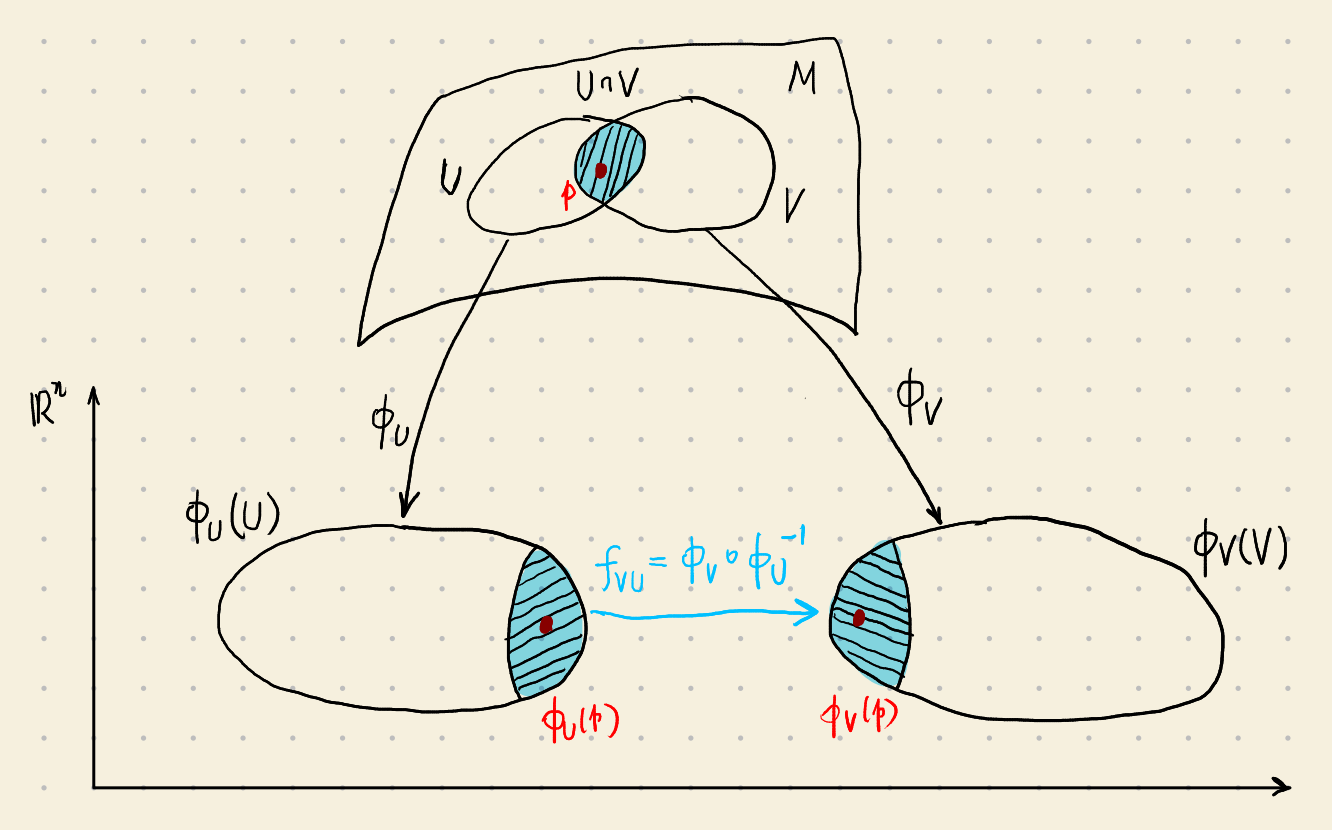
\includegraphics[width=0.8\textwidth, height=\textheight, keepaspectratio]{figures/manifold-draft}
  \caption{}
  \label{fig:manifold}
\end{figure}

\begin{Definition}[Differentiable manifold]
  Let $M$ be a $n$-dimensional manifold. A topology can be defined for $M$ from the local
  coordinate map like this: a subset $W$ of $M$ is open if $\forall p \in W$, there exists
  a coordinate chart $(U, \phi_U)$ such that $p \in U$ and $U$ is contained in $W$
  \footnote{Remember in the Definition \ref{def:manifold}, the image of a coordinate map
    $\phi_U$ is an open set in $\mathbb{R}^n$.}. If such induced topology is Hausdorff and
  $M$ has a countable base, $M$ is called a $n$-dimensional differentiable manifold.
\end{Definition}

Before we have another description of manifold when $M$ is given a topology, we
need to have the following definitions.

\begin{Definition}[Homeomorphism]
  Let $X$ and $Y$ be topological spaces and let $f: X \rightarrow Y$ be a
  bijection. If $f$ and its inverse $f^{-1}$ are both continuous, then $f$ is a
  homeomorphism between $X$ and $Y$.
\end{Definition}

\comment{We say that $X$ and $Y$ are topologically the same.}

\begin{Definition}[Differentiable homeomorphism]
  Let $f: X \rightarrow Y$ be a homeomorphism between topological spaces $X$ and $Y$. If
  $f$ is differentiable, then $f$ is called a differentiable homeomorphism, i.e. $f$ is
  differentiable, while $f^{-1}$ is continuous and may not be differentiable.
\end{Definition}

\begin{Definition}[Diffeomorphism]
  Let $f: X \rightarrow Y$ be a homeomorphism between topological spaces $X$ and
  $Y$. If both $f$ and $f^{-1}$ are differentiable, then $f$ is called a
  diffeomorphism.
\end{Definition}

With the assistance of inverse function theorem, a differentiable homeomorphism can be
locally \textit{upgraded} to a diffeomorphism.

\begin{Theorem}[Inverse function theorem]
  \label{theo:inv-func}
  Let $f: U \rightarrow V$ be a continuous and differentiable bijective map with
  its inverse $f^{-1}$. Let $F_{*}$ be the Jacobi map of $f$. If $\det{F_{*}}
  \neq 0$ at $p \in U$, then $\exists$ $f(p)$'s neighborhood $W \subset V$
  such that $f^{-1}\big\vert_{W}$ is continuous and differentiable.
\end{Theorem}

\comment{$f$ is a local diffeomorphism on $f^{-1}(W)$.}

\begin{Proposition}
  \label{prop:jacobi-and-diffeomorphism}
  Let $f: X \rightarrow Y$ be a differentiable homeomorphism between $X$ and
  $Y$. Let $F_{*}$ be the Jacobi map of $f$. If $\forall p \in X$, $\det{F_{*}}
  \neq 0$, then $f$ is a diffeomorphism.
\end{Proposition}

When a topology is defined for $M$, we will show that when the following
conditions are satisfied, $M$ is also a manifold.

\begin{Proposition}[Manifold with a topology: local diffeomorphism]
  \label{prop:local-diffeomorphism-and-manifold}
  Let $M$ have an open covering $M=U \bigcup V \bigcup \cdots$. For each open
  subset $U$ in the covering, we require that $\exists \phi_U: U \rightarrow
  \phi_U(U) \subset \mathbb{R}^n$ is a diffeomorphism, then $M$ is a manifold.
\end{Proposition}

\begin{Proof}
  $\phi_U$ is a diffeomorphism, so it is a one-to-one correspondence between $U$ and an
  open subset of $\mathbb{R}^n$. Both $\phi_U$ and its inverse $\phi_U^{-1}$ are
  continuous and differentiable bijections. This holds for each open subset in the
  covering.

  We have $\phi_U^{-1}(\phi_U(U \cap V)) = U \cap V$ and because $U \cap V$ is open and
  $\phi_U^{-1}$ is continuous,
  $\phi_U(U \cap V)=(\phi_U^{-1})^{-1}(U \cap V) = \phi_U(U \cap V)$ is open.
  
  In addition, we know that
  \begin{enumerate}
  \item the composition of two bijections is bijective,
  \item the composition of two continuous functions is continuous,
  \item the composition of two differentiable functions is differentiable,
  \end{enumerate}
  so the overlap map $f_{VU}$ and its inverse $f_{UV}$ are both bijective, continuous and
  differentiable. Therefore, the overlap map $f_{VU}$ is differentiable.

  \textbf{In summary, the existence of a local diffeomorphism on each coordinate patch
    ensures that $M$ is a manifold.}
\end{Proof}

\begin{Proposition}[Manifold with a topology: local differentiable homeomorphism]
  Let $M$ have an open covering $M=U \bigcup V \bigcup \cdots$. For each open subset $U$
  in the covering, we require that
  $\exists \phi_U: U \rightarrow \phi_U(U) \subset \mathbb{R}^n$ is a differentiable
  homeomorphism and $\forall p \in U$ its Jacobian $\det{\phi_U^{*}} \neq 0$, then $M$ is
  a manifold.
\end{Proposition}

\begin{Proof}
  This can be proved according to
  \thref{prop:jacobi-and-diffeomorphism} and
  \thref{prop:local-diffeomorphism-and-manifold}.
\end{Proof}

\comment{This is equivalent to say that if there is a differentiable
  homeomorphism that has nonzero Jacobian everywhere on each patch in
  the open covering of $M$, then $M$ itself is a manifold.}

\subsection{Submanifold of manifold}

We already have the definition of a $n$-dimensional submanifold of a Cartesian space
$\mathbb{R}^{n+r}$ in Section \ref{sec:submanifold-of-R}, where the submanifold $M$ is a
geometric entity in $\mathbb{R}^{n+r}$, which has already been assigned coordinates.

According to Definition \ref{def:manifold}, a $n$-dimensional manifold can be covered by
an atlas, which comprises a collection of local coordinate charts. The image of the
coordinate map in each coordinate chart is an open set in $\mathbb{R}^{n}$. Any two
coordinate charts having non-empty overlap can be differentiably transformed
back-and-forth via overlap maps. Therefore, a manifold is locally equivalent
(homeomorphic) to an open set in the Cartesian space. And we can still have a similar
definition for the submanifold of a manifold.

\begin{Definition}[Submanifold of manifold]
  $W^r \subset M^n$ is a submanifold embedded in the manifold $M^n$, if
  $\forall p \in W^r$, there exists a coordinate chart $(U, x) \subset W^r$ containing $p$
  such that $U$ can be represented by a locus:
  $$
  F^1(x) = 0, \cdots, F^{n-r}(x) = 0
  $$
  whose Jacobian matrix $\frac{\pdiff F}{\pdiff x}$ has rank $n-r$ at each point of U.
  Then $W^r$ is a $r$-dimensional submanifold of $M^n$.
\end{Definition}

\begin{Remark}
  As a subspace of the manifold $M^n$, $W^r$ inherits the property of locally homeomorphic
  to an open subset of $\mathbb{R}^n$ and the existence of differentiable overlap maps,
  since $W^r$ is itself a manifold.
\end{Remark}

\begin{Theorem}[Main theorem of submanifold in manifold]
  Let $M^{n+r}$ and $V^r$ be two manifolds. Let $F: M^{n+r} \rightarrow V^r$ and the level
  set $F^{-1}(y_0) = \{x \in M^{n+r} \vert F(x) = y_0\}$ is not empty. If
  $\forall x_0 \in F^{-1}(y_0)$ the Jacobi map
  $F_{*}: M_{x_0}^{n+r} \rightarrow V_{y_0}^r$ is surjective\footnote{The rank of the
    Jacobian matrix is $r$.}, then $F^{-1}(y_0)$ is a $n$-dimensional submanifold of
  $M^{n+r}$.
\end{Theorem}

\subsection{Comparison of several concepts}

\begin{Definition}[Bijection]
  This is the equivalence in the sense of one-to-one and surjective  mapping or correspondence.
\end{Definition}

\begin{Definition}[Isomorphism]
  This is the equivalence in the sense of algebraic structure of group.
\end{Definition}

\begin{Definition}[Homeomorphism]
  This is the equivalence in the sense of topology and requires the
  forward map $f$ and backward map $f^{-1}$ to be continuous. It
  includes bijection.
\end{Definition}

\begin{Definition}[Isometry]
  This is the equivalence in the sense of metric.
\end{Definition}

\begin{Definition}[Differentiable homeomorphism]
  It is a homeomorphism with the forward map $f$ being differentiable.
\end{Definition}

\begin{Definition}[Diffeomorphism]
  It is a homeomorphism with both the forward map $f$ and backward map
  $f^{-1}$ being differentiable.
\end{Definition}

\section{Tangent vector and tangent space}

\begin{Definition}[Tangent vector]
  A tangent vector $v$ at a point $p$ in an $n$-dimensional manifold $M^n$ is defined as a
  physical entity such that for each coordinate chart $(U,x)$ containing $p$, it can be
  represented as an $n$-tuple of real numbers $(v_U^1, \cdots, v_U^n)$\footnote{The
    subscript $U$ indicates the coordinates belong to the chart $U$ and the super script
    $i=1,\cdots,n$ is the coordinate component index.}. The transformation between any two
  of such $n$-tuples derived from two different charts $(U,x_U)$ and $(V,x_V)$ is
  \begin{equation}
    \label{eq:contravariant-transformation}
    v_V^i = \sum_{j=1}^n \frac{\pdiff x_V^i}{\pdiff x_U^j} \Bigg\vert_p v_U^j.
  \end{equation}
\end{Definition}
If we use a column vector to represent $v$, the matrix form of (\ref{eq:contravariant-transformation}) is
\begin{equation}
  \label{eq:contravariant-transformation-matrix-form}
  v_V = \left[ \frac{\pdiff x_{V}}{\pdiff x_U} \right] \Bigg\vert_p v_U,
\end{equation}
where $\left[ \frac{\pdiff x_{V}}{\pdiff x_U} \right]\Big\vert_p$ is the Jacobi matrix of the transition
map $\phi_{VU}$ evaluated at $p$. The transition map $\phi_{VU}$ is
\begin{equation}
  x_V^i = x_V^i(x_U^1, \cdots, x_U^n) \quad (i=1,\cdots,n).
\end{equation}
The Jacobi matrix is
\begin{equation}
  \begin{pmatrix}
    \frac{\pdiff x_V^1}{\pdiff x_U^1} & \cdots & \frac{\pdiff x_V^1}{\pdiff x_U^n} \\
    \vdots & \vdots & \vdots \\
    \frac{\pdiff x_V^n}{\pdiff x_U^1} & \cdots & \frac{\pdiff x_V^n}{\pdiff x_U^n}
  \end{pmatrix}.
\end{equation}

\begin{Definition}[Contravariant transformation]
  The rule in Equation (\ref{eq:contravariant-transformation}) is called
  \emph{contravariant transformation}.
\end{Definition}

\begin{Definition}[Contravariant vector]
  Correspondingly, a vector which transforms with respect to Equation
  (\ref{eq:contravariant-transformation}) is called a \emph{contravariant vector}.
\end{Definition}

\begin{Definition}[Tangent space]
  The collection of all tangent vectors at $p$ in $M^n$ is $\mathbb{R}^n$ rooted at $p$,
  which is called the tangent space. It is represented as $M_p^n$.
\end{Definition}

\subsection{Directional derivative}
\label{sec:directional-derivative}

\begin{Definition}[Directional derivative of a function with respect to a vector]
  Let $\vect{v}$ be a vector and $f$ a scalar function. The directional derivative of $f$
  with respect to $\vect{v}$ at point $p$ is
  \begin{equation}
    \label{eq:directional-derivative-wrt-v}
    D_{\vect{v}}(f) = \frac{d}{dt} \left[ f(p + t\vect{v}) \right] \big\vert_{t=0}.
  \end{equation}
\end{Definition}
This can be understood as the time derivative of $f$ when we move from $p$ with a speed
vector $\vect{v}$. When $\vect{v}$ is a unit speed, i.e. $\norm{v}=1$, this definition is
consistent with the directional derivative in classical calculus.

Assume $f$ is defined on an $n$-dimensional manifold with a coordinate chart $(U, x_{U})$
containing $p$. Since a manifold is locally homeomorphic to $\mathbb{R}^n$, starting from
$p$ then moving with the speed vector $\vect{v}_U$ on the manifold in an infinitesimal
time $dt$ is actually walking along a straight line $x_U(t) = p_U+t\vect{v}_U$. Hence
the above derivative of $f$ can be expanded as
\begin{equation}
  \label{eq:df-in-xu}
  D_{\vect{v}_U}(f) = \sum_{i=1}^n \frac{\pdiff f}{\pdiff x_U^i} \frac{\diff
    x_{U}^i(t)}{\diff t} = \sum_{i=1}^n \frac{\pdiff f}{\pdiff x_U^i}\Bigg\vert_{x_U=p_U} v_U^i.
\end{equation}
If another coordinate chart $(V, x_V)$ is adopted which overlaps with $(U,x_U)$, the
derivative of $f$ can also be written as
\begin{equation}
  \label{eq:df-in-xv}
  D_{\vect{v}_V}(f) = \sum_{i=1}^n \frac{\pdiff f}{\pdiff x_V^i} \frac{\diff
    x_{V}^i(t)}{\diff t} = \sum_{i=1}^n \frac{\pdiff f}{\pdiff x_V^i} \Bigg\vert_{x_V=p_V} v_V^i.
\end{equation}
We can prove that such definition of directional derivative is actually coordinate
independent.

\begin{Proof}[Directional derivative of $f$ is coordinate independent]
  Since $v$ is a tangent vector. Its transformation from $(U,x_U)$ to $(V,x_V)$ requires
  the Jacobi matrix of the transition map $\phi_{VU}$ as below:
  \begin{equation}
    \label{eq:tangent-vector-transform}
    v_V^i = \sum_{j=1}^n \frac{\pdiff x_{V}^i}{\pdiff x_{U}^j} x_U^j \quad (i=1,\cdots,n).
  \end{equation}
  Substitute this transformation into Equation (\ref{eq:df-in-xv}), we have
  $$
  D_{\vect{v}_V}(f) = \sum_{i=1}^n \frac{\pdiff f}{\pdiff x_V^i} \sum_{j=1}^n \frac{\pdiff
    x_{V}^i}{\pdiff x_{U}^j} x_U^j = \sum_{j=1}^n \left( \sum_{i=1}^n \frac{\pdiff f}{\pdiff
      x_V^i} \frac{\pdiff x_{V}^i}{\pdiff x_{U}^j} \right) x_U^j = \sum_{j=1}^n \frac{\pdiff
    f}{\pdiff x_U^j} x_U^j = D_{\vect{v}_U}(f).
  $$
  This is means $D_v(f)$ itself is a \emph{physical entity}, which does not depend on the
  actual coordinate chart we've assigned to the neighborhood of $p$.
\end{Proof}

\begin{Remark}
  The number of coordinate components in $x_U$ does not have to be the same as that of
  $x_V$. And it is neither necessarily the same as the manifold dimension $n$. This is
  because the manifold may be embedded in a higher dimensional space, which needs more
  coordinate components to describe. For example, in the 3D Cartesian space, a 2D sphere
  manifold still needs three coordinates.
\end{Remark}

\subsection{Tangent vector as a differential operator}

As shown in Equation (\ref{eq:directional-derivative-wrt-v}), there is a one-to-one
correspondence between a directional derivative operator and a tangent vector. Therefore,
a tangent vector $v$ rooted at $p$ in a local coordinate chart $(U,x)$ can be
identified with a differential operator:
\begin{equation}
  \label{eq:tangent-vector-as-diff-op}
  v=\sum_j v^j \frac{\pdiff}{\pdiff x^j}\Bigg\vert_p.
\end{equation}
Here $v^j$ is the vector coefficient and the differential operator
$\frac{\pdiff }{\pdiff x^j}\Big\vert_p$ is the corresponding basis vector, which will be
written as $\frac{\vect{\pdiff}}{\vect{\pdiff} x^j}$ in bold typeface from now on or in a
simpler form $\vect{\pdiff} x^j$. Hence, $\left\{ \vect{\pdiff} x^j \right\}_{j=1}^n$ is a
basis of the coordinate chart $(U,x)$. Since the $j$-th component of $v$ in this chart is
just $v^j$, the corresponding basis vector $\vect{\pdiff} x^j$ is numerically the same as
the basis vector $\boldsymbol{e}_j$ of the Cartesian frame $\mathbb{R}^n$, i.e. the $i$-th
component of $\vect{\pdiff}x^j$ is the Kronecker $\delta_j^i$. However, it is not a global
Cartesian frame, but a local Cartesian coordinate frame at $p$ using the coordinate chart
$(U,x)$. More importantly, we should keep in mind that the length of one unit along the
axis $\vect{\pdiff}x^j$ is not necessarily 1, since $\vect{\pdiff}x^j$ may not be a
normalized tangent vector and the metric tensor associated with the coordinate chart may
not be an identity matrix (see Section \ref{sec:metric-tensor} for more information).

\begin{Definition}[Coordinate curve]
  The $i$-th coordinate curve of a coordinate chart $(U,x)$ with $x=(x^1,\cdots,x^n)$ is
  defined as
  \begin{equation}
    \label{eq:coordinate-curves}
    \begin{cases}
      x^i(t)=\text{const} & (i\neq j) \\
      x^j(t)=t
    \end{cases}
    \quad (j=1,\cdots,n).
  \end{equation}
\end{Definition}
This definition means the $j$-th coordinate curve is parameterized by $x^j$ only, while
the other coordinate components are kept constant. The velocity vector of this coordinate
curve at $p$ is the derivative of $x$ at $t=0$, since $p$ is the root point:
\begin{equation}
  \label{eq:tangent-vector-of-coordinate-curve}
  \frac{dx}{dt}\Bigg\vert_{t=0}=(\delta_{j}^1, \cdots, \delta_j^n).
\end{equation}
This is just equal to $\vect{\pdiff}x^j$.

Therefore, the set of velocity vectors of all coordinate curves at $p$ using the
coordinate chart $(U,x)$ forms the basis of the tangent space at $p$, i.e.
$\left\{ \vect{\pdiff} x^j \right\}_{j=1}^n$. This is the same as the results derived from
treating a tangent vector as a differential operator.

If a different coordinate chart $(V,y)$ containing $p$ is adopted, where
$y = (y^1,\cdots,y^{n'})$ may have different number of components from $x$, the basis
$\left\{ \vect{\pdiff}x^j \right\}_{j=1}^n$ in $(U,x)$ can be transformed to the new chart
via the Jacobi matrix of the transition map $\phi_{VU}$, since each basis vector is also a
tangent vector, which should follow the same transformation rule as in
(\ref{eq:tangent-vector-transform}). For the basis vector $\vect{\pdiff}x^j$, the $i$-th
component in the transformed vector is
\begin{equation}
  \label{eq:tangent-space-basis-transform}
  \sum_{k=1}^n \frac{\pdiff y^i}{\pdiff x^k} (\vect{\pdiff} x^j)_k = \sum_{k=1}^n
  \frac{\pdiff y^i}{\pdiff x^k} \delta_k^j = \frac{\pdiff y^{i}}{\pdiff x^{j}} \quad (i=1,\cdots,n').
\end{equation}
Hence, the transformed vector of $\vect{\pdiff}x^j$ is just the $j$-th column of the
Jacobi matrix
$$
\begin{pmatrix}
  \frac{\pdiff y^{1}}{\pdiff x^j} \\
  \vdots \\
  \frac{\pdiff y^{d'}}{\pdiff x^j}
\end{pmatrix}.
$$

\begin{Example}[Coordinate curves of a sphere parameterized by $(r, \varphi, \theta)$]
  Select a neighborhood $U$ of the circle with a latitude $\frac{\pi}{4}$ on the sphere
  which has a radius $r$ and centered at the origin. For example, $U$ can be an open band
  between latitude $\frac{\pi}{5}$ and $\frac{\pi}{3}$. Assign a local coordinate chart
  $(\varphi, \theta)$ to $U$, i.e. the spherical coordinates. Meanwhile, we can still
  assign Cartesian coordinate chart $(x,y,z)$ to $U$. The transformation or transition map
  from $(\varphi,\theta)$ to $(x,y,z)$ is
  \begin{equation}
    \begin{aligned}
      x &= r \cos\varphi \sin\theta \\
      y &= r \sin\varphi \sin\theta \\
      z &= r \cos\theta
    \end{aligned}.
  \end{equation}
  The Jacobi matrix of this map is
  \begin{equation}
    \label{eq:spherical-coordinate-jacobi}
    \begin{pmatrix}
      -r\sin\phi \sin\theta & r\cos\phi \cos\theta \\
      r\cos\phi \sin\theta & r \sin\phi \cos\theta \\
      0 & -r\sin\theta
    \end{pmatrix}.
  \end{equation}
  Then for a point $p$ in $U$, the basis of the tangent space represented in the chart
  $(\varphi, \theta)$ is $\left\{ \vect{\pdiff}\varphi, \vect{\pdiff}\theta \right\}$. In
  the chart $(x,y,z)$, the basis is
  $\left\{ (-r\sin\phi \sin\theta, r\cos\phi \sin\theta, 0)^{\mathrm{T}}, (r\cos\phi
    \cos\theta, r\sin\phi \cos\theta, -r\sin\theta)^{\mathrm{T}} \right\}$. This can be
  visualized in Figure \ref{fig:basis-on-sphere}, where a set of points are selected as
  $p$ whose latitude is $\frac{\pi}{4}$.
  \begin{figure}[htbp]
    \centering
    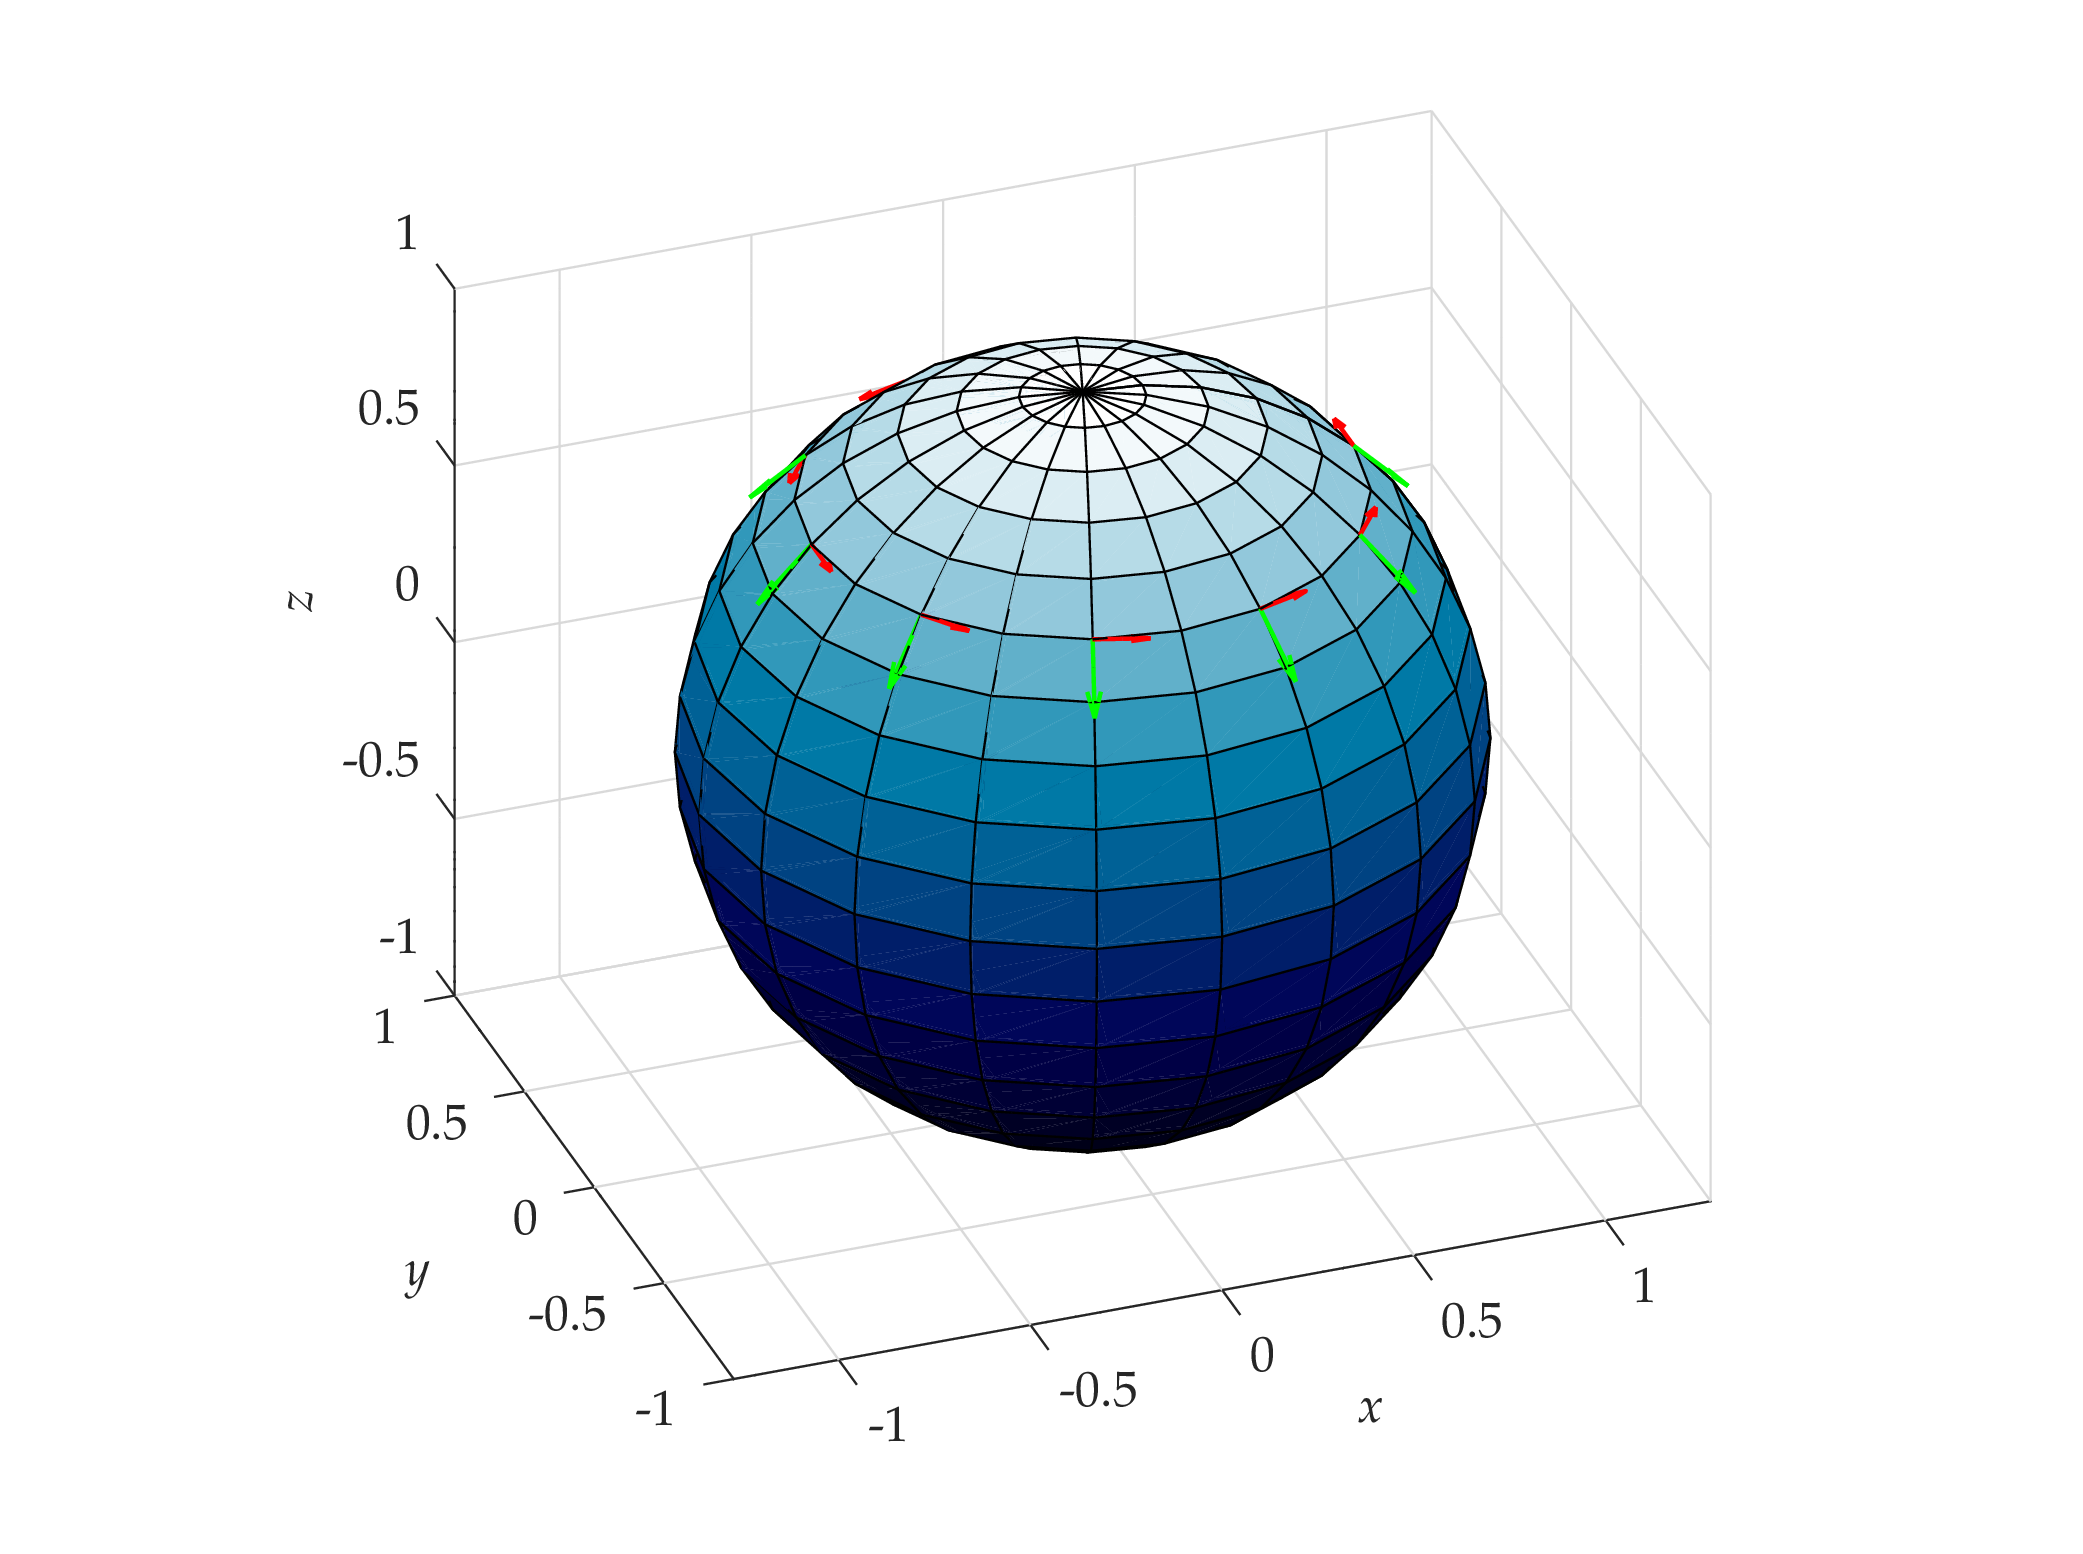
\includegraphics[width=0.7\textwidth, height=\textheight, keepaspectratio]{figures/basis-on-sphere}
    \caption{}
    \label{fig:basis-on-sphere}
  \end{figure}
\end{Example}

The above tangent and velocity vectors of a manifold $M$ can be visualized in an Euclidean
space with a higher dimension, which is ensured by a theorem proposed by Hassler Whitney.
\begin{Theorem}[Hassler Whitney]
  Every $n$-dimensional manifold $M^n$ can be realized as a submanifold of $\mathbb{R}^{2n}$.
\end{Theorem}
This is consistent with our intuition, just imaginge how we understand a 2-sphere in
$\mathbb{R}^3$. However, the definition of tangent vectors for a manifold does not require
such embedding.

\subsection{Relationship between bases of different coordinate charts}

Assume there are two coordinate charts $(U,x_U)$ and $(V,x_V)$ assigned to the tangent
space $M_p^n$. The basis vector using the coordinate chart $(U,x_U)$ is
$\left\{ \vect{\pdiff}x_U^j \right\}$ and the basis vector of $(V,x_V)$ is
$\left\{ \vect{\pdiff}x_V^i \right\}$. Still as before, the number of coordinate
components in $x_U$ and $x_V$ may not be the same. Then we want to know how each basis
vector $\vect{\pdiff}x_V^i$ in $(V,x_V)$ is represented using the basis
$\left\{ \vect{\pdiff}x_U^j \right\}$ in $(U,x_U)$, i.e. we want to compute the expansion
coefficients $a_j$ in the following expression
\begin{equation*}
  \vect{\pdiff}x_V^i = \sum_j a^j \vect{\pdiff}x_U^j.
\end{equation*}
\begin{Remark}
  It should be emphasized that unlike a tangent vector $v$ in $M_p^n$ which is a fixed physical
  entity having multiple representations in different coordinate charts, the basis vectors
  in different coordinate charts like $\vect{\pdiff}x_U^j$ and $\vect{\pdiff}x_V^i$ are
  two different physical entities, i.e. they are usually two different tangent vectors in
  $M_p^n$.
\end{Remark}

Because $\vect{\pdiff}x_V^i$ itself is a tangent vector, its transformation from $(V,x_V)$
into $(U,x_U)$ follows the rule of contravariant transformation in Equation
(\ref{eq:contravariant-transformation}):
\begin{equation*}
  \frac{\pdiff x_U}{\pdiff x_V} (\vect{\pdiff}x_V^i)^{\mathrm{T}}.
\end{equation*}
Note here we've transposed the basis vector $\vect{\pdiff}x_V^i$, because as a convention,
a tangent vector in the matrix form is written as a column vector, while the matrix form
of a basis vector in the tangent space is a row vector. Since $\vect{\pdiff}x_V^i$ is
numerically equivalent to $\vect{e}_i$, the above expression extracts the $i$-th column of
the Jacobi matrix of $\phi_{UV}$. Therefore, the expansion coefficient $a^{j}$ is just the
$j$-th component in this column vector, i.e.
\begin{equation}
  a^j = \frac{\pdiff x_U^j}{\pdiff x_V^i}.
\end{equation}
Hence, the basis vector $\vect{\pdiff}x_V^i$ can be represented as
\begin{equation}
  \label{eq:tangent-vector-basis-relation}
  \vect{\pdiff}x_V^i = \sum_j \frac{\pdiff x_U^j}{\pdiff x_V^i} \vect{\pdiff}x_U^j.
\end{equation}
If we horizontally juxtapose the basis vectors as
$(\vect{\pdiff}x_V^1,\cdots,\vect{\pdiff}x_V^n)$ and
$(\vect{\pdiff}x_U^1,\cdots,\vect{\pdiff}x_U^n)$, the matrix form of the
relationship between the two bases is
\begin{equation}
  (\vect{\pdiff}x_V^1,\cdots,\vect{\pdiff}x_V^n) =
  (\vect{\pdiff}x_U^1,\cdots,\vect{\pdiff}x_U^n) \left[ \frac{\pdiff x_U}{\pdiff x_V} \right].
\end{equation}

\begin{Example}[Basis of spherical coordinate chart]
  \label{exam:spherical-coordinate-basis}
  We still use the spherical coordinate system as an example. Let $(U,x_U)$ be a
  coordinate chart using the Cartesian coordinate frame and $(V,x_V)$ be a coordinate
  chart using the spherical coordinate frame. Then the basis of $(U,x_U)$ is
  $\left\{ \vect{\pdiff}x, \vect{\pdiff}y, \vect{\pdiff}z \right\}$ and the basis of
  $(V,x_V)$ is $\left\{ \vect{\pdiff}\phi, \vect{\pdiff}\theta \right\}$. We want to see
  how $\left\{ \vect{\pdiff}\phi, \vect{\pdiff}\theta \right\}$ is represented in $\left\{
    \vect{\pdiff}x, \vect{\pdiff}y, \vect{\pdiff}z \right\}$. According to Equation
  (\ref{eq:spherical-coordinate-jacobi}),
  \begin{equation}
    \begin{aligned}
      \vect{\pdiff}\phi &= -r\sin\phi \sin\theta \vect{\pdiff}x + r\cos\phi \sin\theta
      \vect{\pdiff}y \\
      \vect{\pdiff}\theta &= r\cos\phi\cos\theta \vect{\pdiff}x + r\sin\phi\cos\theta
      \vect{\pdiff}y - r\sin\theta \vect{\pdiff}z,
    \end{aligned}
  \end{equation}
  i.e. $\vect{\pdiff}\phi$ in the Cartesian frame is just the first column of the Jacobi
  matrix and $\vect{\pdiff}\theta$ is the second column. We also notice that the basis
  vectors $\vect{\pdiff}\phi$ and $\vect{\pdiff}\theta$ are not
  normalized or unit vectors:
  \begin{equation*}
    \begin{aligned}
      \norm{\vect{\pdiff}\phi} &= \sqrt{r^2\sin^2\phi\sin^2\theta +
        r^2\cos^2\phi\sin^2\theta} = \sqrt{r^2\sin^2\theta} = r\sin\theta \\
      \norm{\vect{\pdiff}\theta} &= \sqrt{r^2\cos^2\phi\cos^{2}\theta +
        r^2\sin^2\phi\cos^2\theta + r^2\sin^2\theta} = \sqrt{r^2\cos^2\theta +
        r^2\sin^2\theta} = r.
    \end{aligned}
  \end{equation*}
  Therefore, a normalized basis
  $\left\{ \vect{\pdiff}\hat{\phi}, \vect{\pdiff}\hat{\theta} \right\}$ of the spherical
  coordinate chart is
  $\left\{ \frac{1}{r\sin\theta} \vect{\pdiff}\phi, \frac{1}{r} \vect{\pdiff}\theta
  \right\}$.
\end{Example}

\section{Covector and cotangent space}

\subsection{Concept of duality}
\label{sec:duality-concept}

Taking the familiar inner product in linear algebra as an example (see Figure
\ref{fig:inner-product-of-vectors}). The two vectors $a$ and $b$ have equal status, both
of which are vectors in $\mathbb{R}^n$. The meaning of inner product
$\left\langle a,b \right\rangle$ or $a\cdot b$ is projecting $b$ to $a$.

From the view of measurement, $a$ is the measurement device and $b$ is the object to be
measured. For example, $a$ can be imagined as an electric field meter, $b$ is the electric
field. When the meter is aligned with the electric field line, it registers maximum value.

Adopting the functional analysis point of view, $\left\langle a,b \right\rangle$ or
$a\cdot b$ can be written as $a(b)$. Now $b$ is an element in the space $X$ and
$a: X \rightarrow \mathbb{R}$ is a linear functional or operator in the dual space $X'$.

In computer programming, $a$ can be considered as a functor, while $b$ is the data or
operand to be manipulated.
\begin{figure}[htbp]
  \centering
  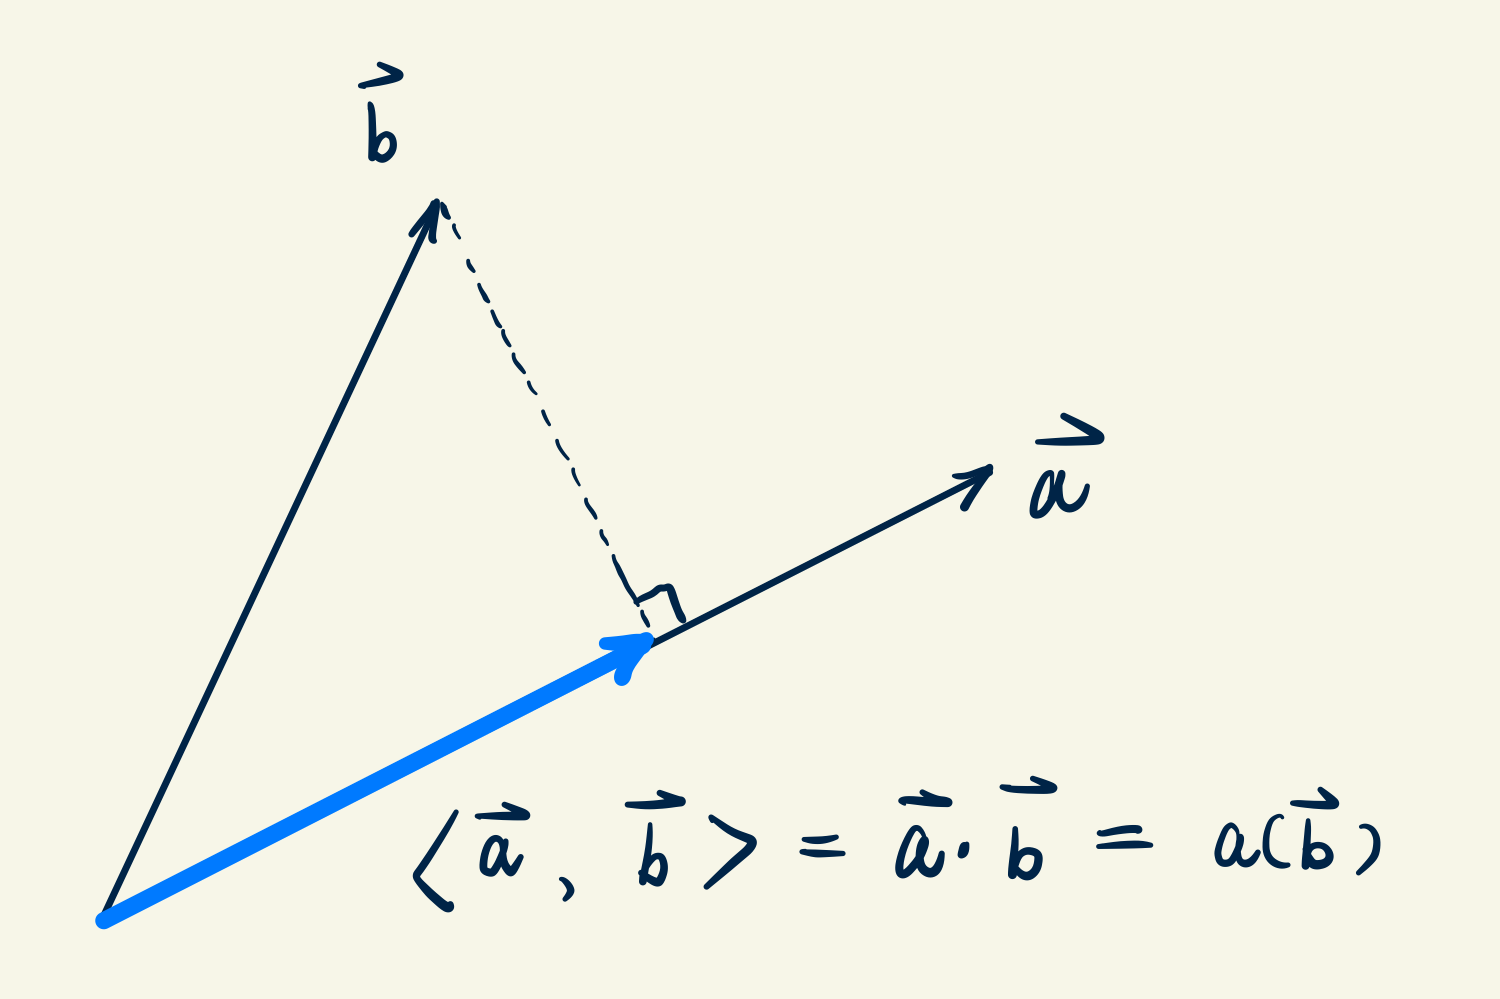
\includegraphics[width=0.5\textwidth, height=\textheight, keepaspectratio]{figures/inner-product-of-vectors-draft}
  \caption{}
  \label{fig:inner-product-of-vectors}
\end{figure}

In essence, $a$ and $b$ have different status and they are dual to each other.

\begin{Example}[Duality]  
  \begin{itemize}
  \item When we compute the inner product using matrix multiplication, $a$ is a row vector
    and $b$ is a column vector. Such difference indicates they are different types of
    vectors.
  \item Ket $|\psi\rangle$ and bra $\langle \varphi |$ in quantum mechanics.
    $\langle \varphi |$ is in the dual space and $|\psi\rangle$ is in the original space.
  \item Inner product of two functions $\int_\Omega u(x)v(x) dx$. $u$ is in the dual space,
    which defines an integral operator, the kernel. $v$ is in the original space to be
    transformed.
  \end{itemize}
\end{Example}

\subsection{Linear functional and dual space}

\begin{Definition}[Linear functional]
  \label{def:linear-functional}
  Let $X$ be a linear space. If the map $f: X \rightarrow \mathbb{R}$ is a linear
  operator, i.e.
  $$
  \begin{aligned}
    f(x + y) &= f(x) + f(y) \quad \forall x, y \in X \\
    f(\alpha x) &= \alpha f(x) \quad \forall x \in X, \alpha \in \mathbb{R}
  \end{aligned},
  $$
  $f$ is a linear functional on $X$.
\end{Definition}

\begin{Definition}[Algebraic dual space]
  \label{def:alg-dual}
  Let $X$ be a linear space. The algebraic dual space $X^{*}$ of $X$ is the collection of
  all linear functionals on $X$. $X^{*}$ is also a linear space, which satisfies
  \begin{equation*}
    \begin{aligned}
      (\alpha+\beta)(v) &= \alpha(v) + \beta(v) \\
      (c\alpha)(v) &= c\alpha(v)
    \end{aligned}
    \quad \forall \alpha,\beta\in X^{*}, v\in X, c\in \mathbb{R}
  \end{equation*}
\end{Definition}

\begin{Definition}[Bounded linear functional]
  \label{def:bounded-linear-functional}
  Let $X$ be a linear space and assigned with a norm $\norm{\cdot}$. $f$ is a bounded
  linear functional on $X$, if for all $x$ in $X$,
  $$
  \abs{f(x)} \leq C \norm{x},
  $$
  where $C$ is a finite constant.
\end{Definition}

\begin{Definition}[Dual space]
  Let $X$ be a linear space and assigned with a norm $\norm{\cdot}$. The dual space $X'$
  of $X$ is the set of all bounded linear functionals on $X$.
\end{Definition}

\subsection{Basis of dual space}

\begin{Definition}[Projection operator]
  A projection operator $\sigma^i: X \rightarrow \mathbb{R}$ is defined as
  \begin{equation}
    \label{eq:projection-operator}
    \sigma^i(\vect{e}_j) = \delta^i_j,
  \end{equation}
  where $\vect{e}_j$ is the $j$-th basis vector of the linear space $X$.
\end{Definition}

For all $v\in X$,
\begin{equation*}
  \sigma^i(v) = \sigma^{i}\left( \sum_j\vect{e}_jv^j \right) = \sum_j
  \sigma^i(\vect{e}_j) v^j = \sum_j\delta^i_j v^j = v^i.
\end{equation*}
This means the projection operator $\sigma^i$ extracts the $i$-th component of the
vector $v$, i.e. it projects $v$ to the $i$-th coordinate axis.

\begin{Proposition}
  Let $X$ be an $n$-dimensional linear space and $X^{*}$ be its dual space. The projection
  operators $\left\{ \sigma^1,\cdots,\sigma^n \right\}$ are linearly independent and any
  linear operator in $X^{*}$ can be uniquely expanded by $\left\{ \sigma^1,\cdots,\sigma^n
  \right\}$. Hence, $\left\{ \sigma^1,\cdots,\sigma^n \right\}$ is a basis of $X^{*}$.
\end{Proposition}

\subsection{0-form}
\label{sec:0-form}

\begin{Definition}[0-form]
  Let $M^n$ be an $n$-dimensional manifold which contains the point $p$. A scalar function
  $f$ defined on a coordinate chart containing $p$ is called a 0-form.
\end{Definition}

\begin{Definition}[Differential 0-form]
  If the values of a 0-form can be differentiably assigned to each point in all coordinate
  charts covering $M^n$, it is called a differential 0-form.
\end{Definition}

\subsection{Covector (1-form) and cotangent space}
\label{sec:1-form}

\begin{Definition}[Cotangent space]
  Let $M^n$ be an $n$-dimensional manifold which contains the point $p$. $M_p^n$ is the
  tangent space at $p$. The dual space of $M_p^n$ is the called the cotangent space at
  $p$, which is written as $M_p^{n*}$.
\end{Definition}

\begin{Definition}[Cotangent vector, covector or 1-form]
  A linear operator $\alpha: M_p^n \rightarrow \mathbb{R}$ in the cotangent space
  $M_p^{n*}$ is called a cotangent vector or covariant vector or covector or 1-form.
\end{Definition}
Applying a 1-form to a tangent vector, we obtain a scalar value.

\begin{Definition}[Differential 1-form]
  Let a 1-form $\alpha$ in the cotangent space $X^{*}$ be expanded by the basis $\left\{
    \sigma^j \right\}$
  \begin{equation*}
    \alpha = \sum_j a_j(x) \sigma^j,
  \end{equation*}
  where each expansion coefficient $a_j$ depends on the local coordinate $x$. If its
  values are differentiably assigned to each point in the coordinate charts covering
  $M^n$, $\alpha$ is a differential 1-form.
\end{Definition}

Apply $\alpha$ to the $i$-th basis vector $\vect{\pdiff}x^i$ of the tangent space, we
obtain the $i$-th expansion coefficient of $\alpha$:
\begin{equation}
  \label{eq:apply-1-form-to-basis}
  \alpha(\vect{\pdiff}x^i) = \sum_j a_j \sigma^j(\vect{\pdiff}x^i) = \sum_j a_j
  \delta^j_i = a_i.
\end{equation}

\subsubsection{Differential of 0-form is 1-form}

Let $f: M^n \rightarrow \mathbb{R}$ be a 0-form on $M^n$. At point $p$, the basis of the
tangent space $M_p^n$ is $\left\{ \vect{\pdiff}x^j \right\}$ and the basis of the
cotangent space $M_p^{n*}$ is $\left\{ \sigma^i \right\}$.
$df: M_p^n \rightarrow \mathbb{R}$ is the differential of $f$, which is a linear
functional operating on a tangent vector $v$. It is defined to be the same as the
directional derivative of $f$ with respect to $v$ (see Equation
(\ref{eq:directional-derivative-wrt-v}) and (\ref{eq:tangent-vector-as-diff-op})):
\begin{equation}
  \label{eq:df-and-directional-derivative}
  df(v) = D_v(f) = v(f) = df \left( \sum_j v^j \vect{\pdiff}x^j \right) = \sum_j v^j
  df(\vect{\pdiff}x^j) = \sum_j v^j \frac{\pdiff f}{\pdiff x^j}\Bigg\vert_p.
\end{equation}
We can see that applying $df$ to the $j$ basis vector in the tangent space simply returns
the partial derivative of $f$ with respect to $x^j$ evaluated at $p$.

If $f=x^i$, we have
\begin{equation*}
  df(v) = dx^i(v) = \sum_j v^j \frac{\pdiff x^{i}}{\pdiff x^j} = \sum_j v^j \delta^i_j = v^i.
\end{equation*}
This means the operator $dx^i$ extracts the $i$-th component of $v$, which is the same as
the projection operator $\sigma^i$. Therefore, $\left\{ dx^i \right\}$ is the basis of the
dual space.

Assume $df$ can be expanded as $df = \sum_j a_j dx^j$. According to Equation
(\ref{eq:apply-1-form-to-basis}),
$a_j = df(\vect{\pdiff}x^j) = \frac{\pdiff f}{\pdiff x^j} \Big\vert_p$. Hence,
\begin{equation}
  \label{eq:differential-of-0-form}
  df = \sum_j \frac{\pdiff f}{\pdiff x^j}\Bigg\vert_p dx^j.
\end{equation}

\subsubsection{Coordinate transformation of a basis vector in the cotangent space}

Assume there are two coordinate charts $(U,x_U)$ and $(V,x_V)$ such that the point $p$
belongs to their intersection. The basis vector $dx_V^{i}$ of the cotangent space
$M_p^{n*}$ in the chart $(V,x_V)$ can be expanded by the basis
$\left\{ dx_U^1,\cdots,dx_U^n \right\}$ in the chart $(U,x_U)$. Because there is the
differentiable transition map $\phi_{VU}$ from $U$ to $V$, $x_V^i$ is actually a function
of $x_U$. Therefore, according to Equation (\ref{eq:differential-of-0-form}), the
expansion of $dx_V^i$ takes the form
\begin{equation}
  \label{eq:cotangent-basis-transformation}
  dx_V^i=\sum_j \frac{\pdiff x_V^i}{\pdiff x_U^j} dx_U^j.
\end{equation}
Its matrix form is
\begin{equation}
  dx_V = \left[ \frac{\pdiff x_V}{\pdiff x_U} \right]\Bigg\vert_p dx_U,
\end{equation}
where $dx_V = (dx_V^1,\cdots,dx_V^n)^{\mathrm{T}}$ and $dx_U = (dx_U^1,\cdots,dx_U^n)^{\mathrm{T}}$.


\subsubsection{Coordinate transformation of a covector in the cotangent space}
\label{sec:covector-transformation}

Let $\alpha$ be a 1-form in the cotangent space $M_p^{n*}$. In the coordinate chart
$(V,x_V)$, it can be expanded as
\begin{equation*}
  \alpha = \sum_i a_i^V dx_V^i.
\end{equation*}
Substitute Equation (\ref{eq:cotangent-basis-transformation}) for $dx_V^i$, we can get the
expansion of $\alpha$ in the coordinate chart $(U,x_U)$ as below.
\begin{equation*}
  \alpha = \sum_i a_i^V \sum_j \frac{\pdiff x_V^i}{\pdiff x_U^j} dx_U^j = \sum_i\sum_j
  a_i^V \left( \frac{\pdiff x_V^i}{\pdiff x_U^j} \right) dx_U^j = \sum_j \left[ \sum_i
    a_i^V \left( \frac{\pdiff x_V^i}{\pdiff x_U^j} \right) \right] dx_U^j = \sum_j a_j^U dx_U^j,
\end{equation*}
where the expansion coefficient is
\begin{equation*}
  \label{eq:covector-transformation}
  a_j^U = \sum_i a_i^V \left( \frac{\pdiff x_V^i}{\pdiff x_U^j} \right).
\end{equation*}
Its matrix form is
\begin{equation}
  a^U = a^V \left[ \frac{\pdiff x_V}{\pdiff x_U} \right],
\end{equation}
where $a^U = (a_1^U,\cdots,a_n^U)$ and $a^V = (a_1^V,\cdots,a_n^V)$,
$\left[ \frac{\pdiff x_V}{\pdiff x_U} \right]$ is the Jacobi matrix of the transition map
$\phi_{VU}$. Similarly,
\begin{equation}
a^V = a^U \left[ \frac{\pdiff x_U}{\pdiff x_V} \right].
\end{equation}

The above coordinate transformation is called the \emph{covariant transformation}.

\subsubsection{Relationship between Jacobi matrices}

We've already met two Jacobi matrices $\left[ \frac{\pdiff x_V}{\pdiff x_U} \right]$ and
$\left[ \frac{\pdiff x_U}{\pdiff x_V} \right]$. The former is the Jacobi matrix of the
transition map $\phi_{VU}$ and the latter is that of the map $\phi_{UV}$. Here we should
emphasize that the number of coordinate components in the chart $(U,x_U)$ may be different
from that of $(V,x_V)$. Moreover, neither of them is necessarily equal to the manifold
dimension $n$. If $(U,x_U)$ has $m$ coordinate components and $(U,x_V)$ has $n$ coordinate
components, $\left[ \frac{\pdiff x_V}{\pdiff x_U} \right] \in \mathbb{R}^{n\times m}$ and
$\left[ \frac{\pdiff x_U}{\pdiff x_V} \right]\in \mathbb{R}^{m\times n}$, i.e. both of
which may be rectangular matrices and have no inverse matrices.

The product of these two matrices are
\begin{equation}
  \left[ \frac{\pdiff x_V}{\pdiff x_U} \right] \cdot \left[ \frac{\pdiff x_U}{\pdiff x_V}
  \right] = \left\{ \sum_k \frac{\pdiff x_V^i}{\pdiff x_U^k} \frac{\pdiff x_U^k}{\pdiff
      x_V^j} \right\}_{ij} = \frac{\pdiff x_V^i}{\pdiff x_V^j} = \left\{ \delta^i_j
  \right\}_{ij} = I_n.
\end{equation}
Similarly,
\begin{equation}
  \left[ \frac{\pdiff x_U}{\pdiff x_V} \right] \cdot \left[ \frac{\pdiff x_V}{\pdiff x_U} \right] = I_m.
\end{equation}

\subsection{Conventions for super and subscripts}

This section summarizes the conventions for superscripts and subscripts used to indicate
the component of a vector and the index of a basis vector in both tangent space and
cotangent space.

Let $v$ be a tangent vector in the tangent space $M_p^n$ and $\alpha$ a cotangent vector
in the cotangent space $M_p^{n*}$. The basis of $M_p^n$ is
$\left\{ \vect{\pdiff}x^i \right\}_{i=1}^n$. The basis of $M_p^{n*}$ is
$\left\{ dx^i \right\}_{i=1}^n$. Superscripts are adopted for
\begin{enumerate}
\item a component of the tangent vector $v$: $v^i$
\item index of a basis vector in the tangent space: $\vect{\pdiff}x^i$. \emph{N.B. The
    superscript $i$ used here is only formal. In fact, $\vect{\pdiff}x^i$ is short for
    $\frac{\pdiff}{\pdiff x^i}$. The superscript $i$ assigned to $x$ appears in the
    denominator, which can be considered as a subscript to index the basis vectors.}
\item index of a basis vector in the cotangent space: $dx^i$
\end{enumerate}
Subscripts are adopted for a component of the covariant vector $\alpha$: $a_i$.

When a vector component or basis vector has been assigned a superscript (subscript), we
can explicitly specify the coordinate chart this entity is using via the unused subscript
(superscript). For example, $v_U^{i}$ is the $i$-th component of the tangent vector $v$,
when the coordinate chart $(U,x_U)$ is adopted. $a_i^U$ is the $i$-th component of the
cotangent vector $\alpha$ and $\vect{\pdiff}x_U^i$ is the $i$-th basis vector in this
chart.

The reason for bothering with the above conventions is to use these formal symbols to
explicitly embody the duality between a tangent space and a cotangent space.

\subsection{Conventions for row and column vectors}

This section summarizes the conventions for using row or column vectors to represent
tangent and cotangent vectors as well as basis vectors in matrix form.

Row vectors are adopted for
\begin{itemize}
\item a covariant vector $\alpha$
\item a basis vector $\vect{\pdiff}x^i$ of the tangent space
\end{itemize}
Column vectors are adopted for
\begin{itemize}
\item a tangent vector $v$
\item a basis vector $dx^i$ of the cotangent space
\end{itemize}

Like sub and superscripts, row and column vectors are adopted to explicitly embody the
duality between a tangent space and a cotangent space.

\section{Tensor and differential forms}

\subsection{Inner product and metric tensor}
\label{sec:metric-tensor}

In a same coordinate chart $(x)$ containing $p$, the inner product of two tangent vectors
$a$ and $b$ in $M_p^n$ is
\begin{equation}
  \label{eq:inner-product}
  \left\langle a,b \right\rangle = \left\langle \sum_i a^i \vect{\pdiff}x^i, \sum_j b^j
    \vect{\pdiff}x^j \right\rangle = \sum_i\sum_j a^i b^j \left\langle \vect{\pdiff}x^i,
    \vect{\pdiff}x^j \right\rangle.
\end{equation}

\begin{Definition}[Metric tensor]
  \label{def:metric-tensor}
  $g_{ij} \coloneqq \left\langle \vect{\pdiff}x^i, \vect{\pdiff}x^j \right\rangle$ is
  called the metric tensor.
\end{Definition}

\begin{Definition}[Riemann metric, Riemann manifold]
  Let $M^n$ be an $n$-dimensional manifold. If for all $p$ in $M^n$, the tangent space
  $M_p^n$ is differentiably assigned a positive definite inner product, i.e. the matrix
  form $G$ of the metric tensor $g_{ij}$ is positive definite, the manifold $M^n$ has a
  Riemann metric and it is a Riemann manifold.
\end{Definition}

The inner product of two tangent vectors in matrix form is
\begin{equation}
  \left\langle a,b \right\rangle = a^T G b.
\end{equation}

According to the section \ref{sec:duality-concept}, the inner product can also be
considered as the application of a covector to a tangent vector. Let $\alpha$ be a
covector in $M_p^{n*}$ and define $\alpha(b) = \left\langle a, b \right\rangle$. This
means the tangent vector $a$ determines or defines a covector $\alpha$.

\begin{Theorem}[Riesz representation theorem]
  Let $X$ be a Hilbert space and $f$ be a bounded linear functional on $X$, i.e.
  $f \in X'$. There exists a unique vector $a$ in $X$, such that for all $b$ in $X$,
  $f(b) = \left\langle a, b \right\rangle$ and $\norm{f} = \norm{a}$.
\end{Theorem}

\subsection{Relationship between metric tensors in different coordinate charts}

Similar to a basis vector of a tangent space, metric tensors in different coordinate
charts are different entities instead of a single fixed entity which has different
numerical representations under different coordinate charts. According to Definition
\ref{def:metric-tensor}, the metric tensor depends on the basis vectors of the tangent
space. Therefore, using Equation (\ref{eq:tangent-vector-basis-relation}), we can obtain
the relationship between metric tensors in different coordinate charts.

Let $(U,x_U)$ and $(V,x_V)$ be two coordinate charts containing the point $p$. In the
neighborhood of $p$, the metric tensor can be represented as
\begin{equation*}
  g_{ij}^V = \left\langle \vect{\pdiff}x_V^i, \vect{\pdiff}x_V^j \right\rangle
\end{equation*}
using the chart $(V,x_V)$. Or it can be represented as
\begin{equation*}
  g_{rs}^U = \left\langle \vect{\pdiff}x_U^r, \vect{\pdiff}x_U^s \right\rangle
\end{equation*}
in the chart $(U,x_U)$. According to Equation (\ref{eq:tangent-vector-basis-relation}), we
have
\begin{equation*}
  \vect{\pdiff}x_V^i = \sum_r \frac{\pdiff x_U^r}{\pdiff x_V^i} \vect{\pdiff}x_U^r
\end{equation*}
and
\begin{equation*}
  \vect{\pdiff}x_V^j = \sum_s \frac{\pdiff x_U^s}{\pdiff x_V^j} \vect{\pdiff}x_U^s.
\end{equation*}
Then
\begin{equation}
  \label{eq:metric-tensor-transformation}
  g_{ij}^V = \left\langle \sum_r \frac{\pdiff x_U^r}{\pdiff x_V^i} \vect{\pdiff}x_U^r,
    \sum_s \frac{\pdiff x_U^s}{\pdiff x_V^j} \vect{\pdiff}x_U^s \right\rangle =
  \sum_r\sum_s \frac{\pdiff x_U^r}{\pdiff x_V^i} \frac{\pdiff x_U^s}{\pdiff x_V^j}
  \left\langle \vect{\pdiff}x_U^r, \vect{\pdiff}x_U^s \right\rangle = \sum_r\sum_s
  \frac{\pdiff x_U^r}{\pdiff x_V^i} \frac{\pdiff x_U^s}{\pdiff x_V^j} g_{rs}^U.
\end{equation}
Its matrix form is
\begin{equation}
  \label{eq:metric-tensor-transformation-matrix-form}
  G^V = \left[ \frac{\pdiff x_U}{\pdiff x_V} \right]^{\mathrm{T}} G^U \left[ \frac{\pdiff
      x_U}{\pdiff x_V} \right] = J_{UV}^{\mathrm{T}} G^U J_{UV}.
\end{equation}

\begin{Example}[Metric tensor of spherical coordinate chart]
  \label{exam:spherical-coordinate-metric-tensor}
  Let $(U,x_U)$ be a coordinate chart using the Cartesian coordinate frame and $(V,x_V)$
  be a coordinate chart using the spherical coordinate frame. Then the basis of $(U,x_U)$
  is $\left\{ \vect{\pdiff}x, \vect{\pdiff}y, \vect{\pdiff}z \right\}$ and the basis of
  $(V,x_V)$ is $\left\{ \vect{\pdiff}\phi, \vect{\pdiff}\theta \right\}$. The metric
  tensor $G^U$ of $(U,x_U)$ is simply a $3\times 3$ identity matrix. Hence, the metric
  tensor $G^V$ of $(V,x_V)$ is
  \begin{equation}
    \label{eq:spherical-coordinate-metric-tensor}
    G^V = J_{UV}^{\mathrm{T}} J_{UV} = \ifx\endpmatrix\undefined\pmatrix{\else\begin{pmatrix}\fi r^2\,
        \sin ^2\theta&0\cr 0&r^2\cr 
        \ifx\endpmatrix\undefined}\else\end{pmatrix}\fi.
  \end{equation}
  Because $G^V$ is a diagonal matrix but not an identity matrix, the spherical coordinate
  frame is orthogonal but not normalized. When $r=1$, the basis vector
  $\vect{\pdiff}\theta$ has unit length but $\vect{\pdiff}\phi$ usually does not.
  $\vect{\pdiff}\phi$ only has unit length when $\theta=\frac{\pi}{2}$, i.e. at the
  equator.
\end{Example}

\subsection{Transformation between tangent vector and covector via metric tensor}

Assume the covector $\alpha$ above can be expanded as
\begin{equation*}
  \alpha = \sum_j \alpha_j dx^j = \sum_j \alpha(\vect{\pdiff}x^j) dx^j = \sum_j
  \left\langle a, \vect{\pdiff}x^j \right\rangle dx^j.
\end{equation*}
If the tangent vector $a$ is expanded as $a = \sum_i a^i \vect{\pdiff}x^i$, we have
\begin{equation*}
  \alpha = \sum_j \left\langle \sum_i a^i \vect{\pdiff}x^i, \vect{\pdiff}x^j \right\rangle
  dx^j = \sum_j\sum_i a^i \left\langle \vect{\pdiff}x^i, \vect{\pdiff}x^j \right\rangle
  dx^j = \sum_j\sum_i a^i g_{ij} dx^j = \sum_j \left( \sum_i a^i g_{ij} \right) dx^j.
\end{equation*}
Therefore, the expansion coefficient of the covector $\alpha$ is
\begin{equation}
  \alpha_j = \sum_i a^i g_{ij}.
\end{equation}
Because the inner product is symmetric with respect to its two operands, so that $g_{ij} = g_{ji}$.
And we prefer the following equivalent formulation of $\alpha_j$
\begin{equation}
  \alpha_j = \sum_i g_{ji} a^i.
\end{equation}
This is because according to the convention, the tangent $a$ vector is represented as a
column vector, while the metric tensor $g_{ji}$ is represented as a matrix. Then the
transformation from the tangent vector $a$ to the covector $\alpha$ can be written as
\begin{equation}
  \alpha = (G a)^{\mathrm{T}} = a^{\mathrm{T}} G.
\end{equation}

On the other hand, the transformation from a covector to its associated tangent vector is
\begin{equation}
  a =  G^{-\mathrm{T}} \alpha^{\mathrm{T}} = G^{-1} \alpha^{\mathrm{T}}.
\end{equation}
Here $G^{-1}$ is an another tensor, whose entry is $g^{ij}$. Therefore
\begin{equation}
  a^i = \sum_{j} g^{ij} \alpha_j.
\end{equation}

\begin{Definition}[Flat operator $\flat$]
  \label{def:flat-operator}
  The operator which transforms a tangent vector to the associated cotangent vector is the
  flat operator $\flat$.
\end{Definition}

\begin{Definition}[Sharp operator $\sharp$]
  \label{def:sharp-operator}
  The operator which transforms a cotangent vector to the associated tangent vector is the
  sharp operator $\sharp$.
\end{Definition}

The flat operator $\flat$ and the sharp operator $\sharp$ are inverse to each other.

\subsection{Relationship between the differential of $f$ and its gradient}

According to Equation (\ref{eq:df-and-directional-derivative}), the differential of a
0-form $f$ is a 1-form $df$. When $df$ is applied to a tangent vector $v$, the returned
scalar value is the directional derivative of $f$ with respect to $v$. In classical
calculus, this is just the projection of the gradient of $f$ to the vector $v$. Hence, the
following definition of the gradient operator is consistent with that learned in calculus.

\begin{Definition}[Gradient operator $\nabla$]
  \label{def:gradient-operator}
  Let $M_p^n$ be the tangent space at $p$ of the manifold $M^n$. $f$ is a 0-form and $df$
  is its differential. For any tangent vector $v$ in $M_p^n$, the gradient operator
  $\nabla$ is defined as
  \begin{equation}
    \label{eq:gradient-operator}
    df(v) = \left\langle \nabla f, v \right\rangle.
  \end{equation}
  Applying $\nabla$ to the 0-form $f$ returns a vector in the tangent space.
\end{Definition}
Compare
\begin{equation*}
  df(v) = \sum_j \frac{\pdiff f}{\pdiff x^j} v^j
\end{equation*}
and
\begin{equation*}
  \left\langle \nabla f, v \right\rangle = \sum_i\sum_j \left( \nabla f \right)^i v^j
  g_{ij} = \sum_j \left( \sum_i \left( \nabla f \right)^i g_{ij} \right) v^j,
\end{equation*}
we have the relationship between the components of the 1-form $df$ and the tangent vector
$\nabla f$
\begin{equation*}
  \frac{\pdiff f}{\pdiff x^j} = \sum_i \left( \nabla f \right)^i g_{ij}.
\end{equation*}
Because the metric tensor is symmetric, $g_{ij} = g_{ji}$,
\begin{equation}
  \label{eq:gradient-to-df}
  \frac{\pdiff f}{\pdiff x^j} = \sum_i g_{ji} \left( \nabla f \right)^i.
\end{equation}
Swapping the subscripts is to derive the following matrix form,
\begin{equation}
  df^{\mathrm{T}} = G \nabla f,
\end{equation}
where $df$ is a row vector and $\nabla f$ is a column vector.

On the other hand,
\begin{equation}
  \label{eq:df-to-gradient}
  \left( \nabla f \right)^i = \sum_j g^{ij} \frac{\pdiff f}{\pdiff x^{i}}
\end{equation}
with the matrix form
\begin{equation}
  \nabla f = G^{-1} df^{\mathrm{T}}.
\end{equation}

According to Definition \ref{def:flat-operator} and \ref{def:sharp-operator},
\begin{equation}
  df = \flat(\nabla f), \; \nabla f = \sharp(df).
\end{equation}

\begin{Example}[Gradient vector on sphere manifold $S^2$]
  According to Example \ref{exam:spherical-coordinate-metric-tensor}, the matrix form of
  the metric tensor $G$ in the spherical coordinate chart is Equation
  (\ref{eq:spherical-coordinate-metric-tensor}). If the basis
  $\left\{ \vect{\pdiff}\phi, \vect{\pdiff}\theta \right\}$ is adopted for the tangent space, the matrix form of
  $\nabla f$ is
  \begin{equation}
    \nabla f = \begin{pmatrix}
      \frac{1}{r^2\sin^2\theta} & 0 \\
      0 & \frac{1}{r^2}
    \end{pmatrix}
    \cdot
    \begin{pmatrix}
      \frac{\pdiff f}{\pdiff \phi} \\
      \frac{\pdiff f}{\pdiff \theta}
    \end{pmatrix} = \begin{pmatrix}
      \frac{1}{r^2\sin^2\theta} \frac{\pdiff f}{\pdiff \phi} \\
      \frac{1}{r^2} \frac{\pdiff f}{\pdiff \theta}
    \end{pmatrix}.
  \end{equation}
  Its tangent vector form is
  \begin{equation}
    \nabla f = \frac{1}{r^2\sin^2\theta} \frac{\pdiff f}{\pdiff \phi} \vect{\pdiff}\phi +
    \frac{1}{r^2} \frac{\pdiff f}{\pdiff \theta} \vect{\pdiff}\theta.
  \end{equation}
  If the normalized basis
  $\left\{ \vect{\pdiff}\hat{\phi}, \vect{\pdiff}\hat{\theta} \right\}$ as in Example
  \ref{exam:spherical-coordinate-basis} is adopted, the tangent vector form is
  \begin{equation}
    \nabla f = \frac{1}{r^2\sin^2\theta} \frac{\pdiff f}{\pdiff \phi} r\sin\theta \vect{\pdiff}\hat{\phi} +
    \frac{1}{r^2} \frac{\pdiff f}{\pdiff \theta} r \vect{\pdiff}\hat{\theta} =
    \frac{1}{r\sin\theta} \frac{\pdiff f}{\pdiff \phi} \vect{\pdiff}\hat{\phi} +
    \frac{1}{r} \frac{\pdiff f}{\pdiff \theta} \vect{\pdiff}\hat{\theta}.
  \end{equation}
\end{Example}

\begin{Example}[Gradient vector on ball manifold]
  Compared to the sphere manifold, now the basis of the tangent space in the local
  spherical coordinate chart is
  $\left\{ \vect{\pdiff}r, \vect{\pdiff}\phi, \vect{\pdiff}\theta \right\}$. The Jacobi
  matrix from the spherical coordinate chart to the Cartesian coordinate chart is
  \begin{equation}
    \label{eq:ball-coordinate-jacobi}
    J = \begin{pmatrix}
      \cos\phi \sin\theta & -r\sin\phi \sin\theta & r\cos\phi \cos\theta \\
      \sin\phi \sin\theta & r\cos\phi \sin\theta & r \sin\phi \cos\theta \\
      \cos\theta & 0 & -r\sin\theta
    \end{pmatrix}.
  \end{equation}
  The metric tensor is
  \begin{equation}
    \label{eq:ball-coordinate-metric-tensor}
    G = J^{\mathrm{T}} J = \begin{pmatrix}
      1&0&0 \\
      0&r^2\,\sin ^2\theta&0 \\
      0&0&r^2
    \end{pmatrix}.
  \end{equation}
  The matrix form of $\nabla f$ is
  \begin{equation}
    \nabla f = \begin{pmatrix}
      1 & 0 & 0\\
      0 & \frac{1}{r^2\sin^2\theta} & 0 \\
      0 & 0 & \frac{1}{r^2}
    \end{pmatrix}
    \cdot
    \begin{pmatrix}
      \frac{\pdiff f}{\pdiff r} \\
      \frac{\pdiff f}{\pdiff \phi} \\
      \frac{\pdiff f}{\pdiff \theta}
    \end{pmatrix} = \begin{pmatrix}
      \frac{\pdiff f}{\pdiff r} \\
      \frac{1}{r^2\sin^2\theta} \frac{\pdiff f}{\pdiff \phi} \\
      \frac{1}{r^2} \frac{\pdiff f}{\pdiff \theta}
    \end{pmatrix}.
  \end{equation}
  Its tangent vector form is
  \begin{equation}
    \nabla f = \frac{\pdiff f}{\pdiff r}\vect{\pdiff}r + \frac{1}{r^2\sin^2\theta} \frac{\pdiff f}{\pdiff \phi} \vect{\pdiff}\phi +
    \frac{1}{r^2} \frac{\pdiff f}{\pdiff \theta} \vect{\pdiff}\theta.
  \end{equation}
  Using the normalized basis
  $\left\{ \vect{\pdiff}\hat{r}, \vect{\pdiff}\hat{\phi}, \vect{\pdiff}\hat{\theta}
  \right\}$, where $\vect{\pdiff}\hat{r} = \vect{\pdiff}r$, we have
  \begin{equation}
    \nabla f = \frac{\pdiff f}{\pdiff r}\vect{\pdiff}\hat{r} + \frac{1}{r\sin\theta} \frac{\pdiff f}{\pdiff \phi} \vect{\pdiff}\hat{\phi} +
    \frac{1}{r} \frac{\pdiff f}{\pdiff \theta} \vect{\pdiff}\hat{\theta}.
  \end{equation}
  This is consistent with the result in a classical electrodynamics book such as
  \citep{GriffithsIntroduction1999}.
\end{Example}

\subsection{General definition of tensors}

\subsubsection{Covariant tensor}
\label{sec:covariant-tensor}

1-form introduced in Section \ref{sec:1-form} is a linear functional in the cotangent
(covariant) space, which is dual to the tangent (contravariant) space. The application of
a 1-form to a tangent vector produces a scalar value. The concept of tensor is a
generalization of 1-form. Instead of operating on a single tangent vector and being a
linear functional, an $r$-th rank tensor $Q$ is a \emph{multilinear} functional operating
on $r$ tangent vectors, $v_1, \cdots, v_r$. This sequence \footnote{``Sequence'' means the
  $r$ tangent vectors are ordered.} of $r$ tangent vectors is called a $r$-vector, which
belongs to the Cartesian product of $r$ tangent spaces $M_p^n$, i.e. $\otimes^r M_p^n$.
Then this tensor $Q$ belongs to the dual space of $\otimes^r M_p^n$, i.e.
$\left( \otimes^r M_p^n \right)^*$, which is a Cartesian product of $r$ cotangent spaces
$M_p^{n*}$,
\begin{equation}
  \left( \otimes^r M_p^n \right)^* = \otimes^r M_p^{n*}.
\end{equation}
Because $Q$ belongs to the dual space or product of cotangent spaces, it is called a
covariant tensor.

\begin{Definition}[Covariant tensor]
  An $r$-th rank covariant tensor $Q$ is a multilinear functional operating on the
  Cartesian product $r$ of tangent spaces $\otimes^r M_p^n$, i.e.
  $Q: \otimes^r M_p^n \rightarrow \mathbb{R}$.
\end{Definition}
Therefore, a 1-form can be considered as a rank-1 tensor, which is a degenerate case.

Applying $Q$ to any $v_1, \cdots, v_r$ in $M_p^n$, using multilinearity, we have
\begin{equation}
  \label{eq:covariant-tensor-applied-to-r-vectors-expanded}
  \begin{aligned}
    Q(v_1,\cdots,v_r) &= Q(\sum_{i_1}v_1^{i_1} \vect{\pdiff}x^{i_1}, \cdots,
    \sum_{i_r}v_r^{i_r} \vect{\pdiff}x^{i_r}) \\
    &= \sum_{i_1}v_1^{i_1} Q(\vect{\pdiff}x^{i_1},\cdots,\sum_{i_r}v_r^{i_r}\vect{\pdiff}x^{i_r}) \\
    &= \sum_{i_1}\cdots\sum_{i_r}v_1^{i_1}\cdots v_r^{i_r}
    Q(\vect{\pdiff}x^{i_1},\cdots,\vect{\pdiff}x^{i_r}),
  \end{aligned}
\end{equation}
where we use $i_k$ as the index to iterative over each component of the $k$-th tangent
vector $v_k$ for $k=1,\cdots,r$. Let
$Q_{i_1\cdots i_r}= Q(\vect{\pdiff}x^{i_1},\cdots,\vect{\pdiff}x^{i_r})$, which is the
application of $Q$ to a basis vector of the product tangent space. Using the Einstein
summation notation (i.e. the summation symbol $\sum_{i_k}$ with respect to an index $i_k$
can be omitted whenever there is a pair of subscript $i_k$ and superscript $i_k$ appearing
in the summand), we have
\begin{equation}
  \label{eq:covariant-tensor-applied-to-r-vectors}
  Q(v_1,\cdots,v_r) = v_1^{i_1}\cdots v_r^{i_r} Q_{i_1 \cdots i_r}.
\end{equation}

\begin{Definition}[Tensor product of two covariant tensors]
  Let $Q^1$\footnote{Because the subscript of $Q$ has already been used for specifying
    multi-summation indices, here we use the superscript to label different covariant
    tensors.} be an $r$-th rank covariant tensor and $Q^2$ be an $s$-th rank covariant
  tensor. Their tensor product is an $(r+s)$-th rank covariant tensor which satisfies
  \begin{equation}
    \label{eq:tensor-product-of-covariant-tensors}
    \left( Q^1 \otimes Q^2 \right) (v_{1},\cdots,v_{r}, v_{r+1},\cdots,v_{r+s}) =
    Q^1(v_{1},\cdots,v_{r}) Q^2(v_{r+1},\cdots,v_{r+s}).
  \end{equation}
\end{Definition}

An $r$-th rank covariant tensor $Q$ can also be considered as a \emph{tensor product} of
$r$ 1-forms. Let $\alpha^1,\cdots,\alpha^r$ be $r$ 1-forms in $M_p^{n*}$, their tensor product
is $\otimes_i\alpha^i: \otimes^r M_p^n \rightarrow \mathbb{R}$, which is a multilinear
functional on the Cartesian product of $r$ tangent spaces $M_p^n$. For any
$v_1, \cdots, v_r$ in $M_p^n$,
\begin{equation}
  \left(\otimes_i\alpha^i\right)(v_1,\cdots,v_r) = \prod_i \alpha^i(v_i).
\end{equation}
Apply $\otimes_i\alpha^i$ to $\vect{\pdiff}x^{k_1},\cdots,\vect{\pdiff}x^{k_r}$, we have
\begin{equation}
  \left( \otimes_i\alpha^i \right)(\vect{\pdiff}x^{k_1},\cdots,\vect{\pdiff}x^{k_r}) =
  \prod_i\alpha^i(\vect{\pdiff}x^{k_i}) = \prod_i \alpha_{k_i}^{i}.
\end{equation}
Then expand $\prod_i \alpha^i(v_i)$\footnote{Originally, we may want to expand it like this:
  $\prod_i \alpha^i(v_i) = \prod_i \alpha^i\left( \sum_k v_i^k \vect{\pdiff}x^k \right) =
  \prod_i \sum_k v_i^k \alpha^i(\vect{\pdiff}x^k)$. However, this hides the fact that for
  each multiplier in the product, its summation index is independent from others.
  Therefore, the summation index $k$ for the $i$-th multiplier should have a subscript $i$
  to distinguish it from others.}:
\begin{equation}
  \begin{aligned}
    \prod_i \alpha^i(v_i) &= \prod_i \alpha^i\left( \sum_{k_i}v_i^{k_i}
      \vect{\pdiff}x^{k_i} \right) = \prod_i \sum_{k_i}v_i^{k_i}
    \alpha^i(\vect{\pdiff}x^{k_i}) = \prod_i \sum_{k_i} v_i^{k_i} \alpha_{k_i}^i \\
    &= \sum_{k_1}\cdots\sum_{k_r} v_1^{k_1}\cdots v_r^{k_r}
    \alpha_{k_1}^1\cdots\alpha_{k_r}^r = v_1^{k_1}\cdots v_r^{k_r} \left(
      \otimes_i\alpha^i \right)(\vect{\pdiff}x^{k_1},\cdots,\vect{\pdiff}x^{k_r}).
  \end{aligned}
\end{equation}
This means the construction of a $r$-th rank covariant tensor via tensor product of $r$
1-forms is consistent with Equation (\ref{eq:covariant-tensor-applied-to-r-vectors}).

Since a covariant tensor is constructed from the tensor product of $r$ 1-forms, a basis
vector of the covariant tensor space can be constructed via a tensor product of the bases
for all the cotangent spaces in which the $r$ 1-forms reside. Therefore,
$dx^{i_1}\otimes\cdots\otimes dx^{i_r}$ is a basis vector of the covariant tensor space
and the tensor $Q$ can be represented as
\begin{equation}
  \label{eq:covariant-tensor-expanded-as-tensor-product}
  Q = Q_{i_1\cdots i_r} dx^{i_1}\otimes\cdots\otimes dx^{i_r}.
\end{equation}
It can be shown that this definition of $Q$ is consistent with Equation
(\ref{eq:covariant-tensor-applied-to-r-vectors}) by applying it to $v_1,\cdots,v_r$:
\begin{equation}
  Q(v_1,\cdots,v_r) = Q_{i_1\cdots i_r} dx^{i_1}\otimes\cdots\otimes
  dx^{i_r}(v_1,\cdots,v_r) = Q_{i_1\cdots i_r} dx^{i_1}(v_1)\cdots dx^{i_r}(v_r) =
  Q_{i_1\cdots i_r} v_1^{i_1}\cdots v_r^{i_r}.
\end{equation}
Because the summation indices $i_1,\cdots,i_r$ are independent from each other and each of
them have $n$ terms, the dimension of the covariant tensor space is $n^r$.

\begin{Remark}
  From a programming point of view, the tensor product operation related to an $r$-th rank
  tensor is actually nested $r$ loops.
  \begin{breakablealgorithm}
  \begin{algorithmic}[1]
    \For {$i_1 \coloneqq 1,\cdots,n$}
      \For {$i_2 \coloneqq 1,\cdots,n$}
        \State {$\cdots$}
        \For {$i_r \coloneqq 1,\cdots,n$}
          \State {Compute a component of the tensor.}
        \EndFor
      \EndFor
    \EndFor
  \end{algorithmic}
  \end{breakablealgorithm}
\end{Remark}

\subsubsection{Contravariant tensor}

\begin{Definition}[Contravariant tensor]
  An $s$-th rank contravariant tensor $T$ is a multilinear real valued function on $s$
  1-forms, i.e. $T: \otimes^s M_p^{n*} \rightarrow \mathbb{R}$.
\end{Definition}
Actually, an $s$-th rank contravariant tensor $T$ is also a multilinear functional on the
product of cotangent spaces. A cotangent space is the dual space of a tangent space, which
is the set of all linear functionals on the tangent space. Similarly, the product of
cotangent spaces is the dual space of the product of tangent spaces. Now, the tensor $T$
belongs to the dual space of the product of cotangent spaces, i.e.
$\left( \otimes^s M_p^{n*} \right)^{*}$. Hence it is actually the dual of the dual space
of the product of tangent spaces, i.e. $\left( \otimes^s M_p^n \right)^{**}$. According to
functional analysis theory, the original product of tangent spaces $\otimes^s M_p^n$ is an
embedding into the dual of dual space $\left( \otimes^s M_p^n \right)^{**}$.\footnote{An
  embedding is an injective map, which preserves the linear structure of the space.} When
$\otimes^s M_p^n$ is a finite dimensional space, the embedding is an isomorphism, which
means the map from $\otimes^s M_p^n$ to $\left( \otimes^s M_p^n \right)^{**}$ is bijective
which preserves the linear structure. Therefore, $\otimes^s M_p^n$ and
$\left( \otimes^s M_p^n \right)^{**}$ are identical. In this case, the product space
$\otimes^s M_p^n$ is called a \emph{reflexive} space.

Similar to applying $Q$ to a tuple of tangent vectors, we apply $T$ to $s$ 1-forms
$\alpha^1,\cdots,\alpha^s$,
\begin{equation}
  \label{eq:contravariant-tensor-applied-to-s-1-forms}
  T(\alpha^1,\cdots,\alpha^s) = T(\sum_{i_1}\alpha_{i_1}^1 dx^{i_1}, \cdots,
  \sum_{i_s}\alpha_{i_s}^s dx^{i_s}) = \alpha_{i_1}^1\cdots\alpha_{i_s}^s T^{i_1 \cdots i_s},
\end{equation}
where $T^{i_s\cdots i_s} = T(dx^{i_1},\cdots,dx^{i_s})$ is the application of $T$ to a basis vector of the product
cotangent space.

\begin{Definition}[Tensor product of two contravariant tensors]
  Let $T_1$\footnote{Because the superscript of $T$ has already been used for specifying
    multi-summation indices, here we use the subscript to label different contravariant
    tensors.} be an $r$-th rank contravariant tensor and $T_2$ be an $s$-th rank
  contravariant tensor. Their tensor product is an $(r+s)$-th rank contravariant tensor
  which satisfies
  \begin{equation}
    \label{eq:tensor-product-of-contravariant-tensors}
    \left( T_1 \otimes T_2
    \right)(\alpha^1,\cdots,\alpha^r,\alpha^{r+1},\cdots,\alpha^{r+s}) =
    T_1(\alpha^1,\cdots,\alpha^r) T_2(\alpha^{r+1},\cdots,\alpha^{r+s}).
  \end{equation}
\end{Definition}

$T$ can also be constructed from the tensor product of $s$ tangent vectors. Let
$v_1,\cdots,v_s$ be $s$ tangent vectors in $M_p^n$. Their tensor product is
$\otimes_i v_i: \prod_i M_p^{n*} \rightarrow \mathbb{R}$, which is a multilinear
functional on the product of $s$ cotangent spaces $M_p^{n*}$. For any
$\alpha^1,\cdots,\alpha^s$ in $M_p^{n*}$,
\begin{equation}
  \left( \otimes_i v_i \right)(\alpha^1,\cdots,\alpha^s) = \prod_i v_i(\alpha^i) = \prod_i
  \alpha^i(v_i).
\end{equation}
Apply $\otimes_iv_i$ to the tuple of basis vectors $dx^{k_1},\cdots,dx^{k_s}$, we have
\begin{equation}
  \left( \otimes_i v_i \right)(dx^{k_1},\cdots,dx^{k_s}) = \prod_i v_i(dx^{k_i}) = \prod_i
  dx^{k_i}(v_i) = \prod_i v_i^{k_i}.
\end{equation}
Then expand $\prod_i v_i(\alpha^i)$:
\begin{equation}
  \begin{aligned}
    \prod_i v_i(\alpha^i) &= \prod_i v_i \left( \sum_{k_i}\alpha_{k_i}^i dx^{k_i} \right)
    = \prod_i\sum_{k_i} \alpha_{k_i}^iv_i(dx^{k_i}) = \prod_i\sum_{k_i}\alpha_{k_i}^i
    dx^{k_i}(v_i) \\
    &= \prod_i\sum_{k_i} \alpha_{k_i}^i v_i^{k_i} =
    \sum_{k_1}\cdots\sum_{k_s}\alpha_{k_1}^1\cdots\alpha_{k_s}^s v_1^{k_1}\cdots v_s^{k_s} \\
    &= \alpha_{k_s}^1\cdots\alpha_{k_s}^s \otimes_iv_i(dx^{k_1},\cdots,dx^{k_s}).
  \end{aligned}
\end{equation}
Since a contravariant tensor is constructed from the tensor product of $s$ tangent
vectors, a basis vector of the contravariant tensor space can be represented as the tensor
product of the bases for all the tangent spaces in which the $s$ tangent vectors reside.
Therefore, $\vect{\pdiff}x^{i_1}\otimes\cdots\otimes \vect{\pdiff}x^{i_s}$ is a basis
vector of the contravariant tensor space and the tensor $T$ can be represented as
\begin{equation}
  \label{eq:contravariant-tensor-expanded-as-tensor-product}
  T = T^{i_1\cdots i_s} \vect{\pdiff}x^{i_1}\otimes\cdots\otimes \vect{\pdiff}x^{i_s}.
\end{equation}

\subsubsection{Mixed tensor}

\begin{Definition}[Mixed tensor]
  A mixed tensor $W$, which has contravariant rank $s$ and covariant rank $r$, is a
  multilinear real valued function on $s$ 1-forms and $r$ tangent vectors, i.e.
  $W:\left( \otimes^s M_p^{n*} \right) \otimes \left( \otimes^r M_p^n \right) \rightarrow
  \mathbb{R}$. It is actually the tensor product of an $s$-rank contravariant tensor and
  an $r$-th rank covariant tensor.
\end{Definition}
Hence $W$ belongs to the dual space of the product space
$\left( \otimes^s M_p^{n*} \right) \otimes \left( \otimes^r M_p^n \right)$.

Similar as before, apply $W$ to a basis vector of this product space,
$(dx^{i_1},\cdots,dx^{i_s},\vect{\pdiff}x^{j_1},\cdots,\vect{\pdiff}x^{j_r})$, we obtain
\begin{equation}
  W^{i_1\cdots i_s}_{j_1\cdots j_r} = W(dx^{i_1},\cdots,dx^{i_s},\vect{\pdiff}x^{j_1},\cdots,\vect{\pdiff}x^{j_r}).
\end{equation}
Then
\begin{equation}
  W(\alpha^1,\cdots,\alpha^s,v_1,\cdots,v_r) = \alpha_{i_1}^1\cdots \alpha_{i_s}^s
  W^{i_1\cdots i_s}_{j_1\cdots j_r} v_1^{j_1}\cdots v_r^{j_r}.
\end{equation}
There are altogether $r+s$ summations in this expression.

Similar as the expansion of a covariant or contravariant tensor, a mixed tensor can be
represented as
\begin{equation}
  \label{eq:mixed-tensor-expanded-as-tensor-product}
  W = W^{i_1\cdots i_s}_{j_1\cdots j_r} \vect{\pdiff}x^{i_1}\otimes\cdots\otimes
  \vect{\pdiff}x^{i_s}\otimes dx^{j_1}\otimes\cdots\otimes dx^{j_r}.
\end{equation}

\subsubsection{Conventions for super and subscripts}

This section summarizes the conventions for subscripts and superscripts used to indicate
the component of a tensor.

Generally speaking, a tensor is a multilinear functional on a product space comprising of
a few cotangent spaces and/or tangent spaces. When a component vector in the product space
to be operated by the tensor is covariant, the coefficients of which are indexed by subscripts, then
the tensor coefficients will have a corresponding superscript. On the contrary, when a
component vector in the product space to be operated by the tensor is contravariant, the
coefficients of which are indexed by superscripts, then the tensor coefficients will have
corresponding subscript.

\subsection{Coordinate transformation of tensors}

Because a tensor is the generalization of the concept of a tangent vector and 1-form via
tensor product, its coordinate transformation is also a generalization of the
transformation for a tangent vector (see Section \ref{sec:directional-derivative}) and
1-form (see Section \ref{sec:covector-transformation}).

Let $(U,x_U)$ and $(V,x_V)$ be two coordinate charts having non-empty overlap. We use
indices $r\cdots s$ and $c\cdots d$ for quantities in the chart $(U,x_U)$ and use indices
$i\cdots j$ and $k\cdots l$ for $(V,x_V)$.
\begin{itemize}
\item Coordinate transformation of a covariant tensor
  \begin{equation}
    \label{eq:covariant-tensor-transform}
    Q_{i\cdots j}^V = \left( \frac{\pdiff x_U^r}{\pdiff x_V^i} \right) \cdots \left(
      \frac{\pdiff x_U^s}{\pdiff x_V^j} \right) Q_{r \cdots s}^U
  \end{equation}
\item Coordinate transformation of a contravariant tensor
  \begin{equation}
    \label{eq:contravariant-tensor-transform}
    T_V^{i \cdots j} = \left( \frac{\pdiff x_V^i}{\pdiff x_U^r} \right) \cdots \left(
      \frac{\pdiff x_V^j}{\pdiff x_U^s} \right) T_U^{r \cdots s}
  \end{equation}
\item Coordinate transformation of a mixed tensor
  \begin{equation}
    \label{eq:mixed-tensor-transform}
    \left( W^{i \cdots j}_{k \cdots l} \right)_V = \left( \frac{\pdiff x_V^i}{\pdiff x_U^c} \right)
    \cdots \left( \frac{\pdiff x_V^j}{\pdiff x_U^d} \right) \left( \frac{\pdiff
        x_U^r}{\pdiff x_V^k} \right) \cdots \left( \frac{\pdiff x_U^s}{\pdiff x_V^l}
    \right) \left( W^{c \cdots d}_{r \cdots s} \right)_U
  \end{equation}
\end{itemize}

\subsection{Exterior form and exterior algebra}

\begin{Definition}[(Exterior) $k$-form]
  A $k$-form $\alpha$ is an antisymmetric (also called skew symmetric) $k$-rank covariant
  tensor, which satisfies
  \begin{equation}
    \alpha(v_1, \cdots, v_r, \cdots, v_s, \cdots, v_k) = -\alpha(v_1, \cdots, v_s, \cdots, v_r,
    \cdots, v_k).
  \end{equation}
\end{Definition}

\begin{Remark}
  When there are two equal vectors, such as $v_r = v_s$, in the $k$-vector
  $(v_1,\cdots,v_k)$, we have $\alpha(v_1,\cdots,v_k) = 0$.
  
  A 0-form is a degenerate case of a general $k$-form, where there are no tangent vectors
  to be operated. Because there are no tangent vectors for us to swap any two of them, the
  above definition of antisymmetry is \emph{vacuously} true\footnote{When the precondition
    required by a statement does not exist, the statement is still considered as vacuously
    true (see \citet{MunkresTopology2000})}.
    
  A 1-form is a degenerate case of a general $k$-form, where there is only one tangent
  vector to be operated. Similar to 0-forms, the antisymmetry for 1-forms is also
  vacuously true.
\end{Remark}

According to Equation (\ref{eq:covariant-tensor-applied-to-r-vectors-expanded}), applying
an $r$-th rank covariant tensor $Q$ to an $r$-vector can be expanded as a multi-summation
due to its multilinearity, where there are altogether $n^r$ terms in the sum. Now for a
$k$-form $\alpha$, which is also a $k$-th rank covariant tensor, applying it to
a $k$-vector $(v_1,\cdots,v_k)$ can be similarly expanded as
\begin{equation}
  \label{eq:k-form-applied-to-k-vector-expanded}
  \alpha(v_{1},\cdots,v_{k}) = \alpha \left(
    \sum_{i_1}v_1^{i_1}\vect{\pdiff}x^{i_1},\cdots,\sum_{i_k}v_k^{i_k}\vect{\pdiff}x^{i_k}
  \right) = \sum_{i_1}\cdots\sum_{i_k}v_1^{i_1}\cdots v_k^{i_k}
  \alpha(\vect{\pdiff}x^{i_1},\cdots, \vect{\pdiff}x^{i_k}).
\end{equation}
Moreover, due to the antisymmetry of $\alpha$, some terms in the above multi-summation can
be combined. For example, because
\begin{equation}
  \alpha(\vect{\pdiff}x^{i_1},\cdots,\vect{\pdiff}x^{i_r},\cdots,\vect{\pdiff}x^{i_s},\cdots,\vect{\pdiff}x^{i_k})
  =
  -\alpha(\vect{\pdiff}x^{i_1},\cdots,\vect{\pdiff}x^{i_s},\cdots,\vect{\pdiff}x^{i_r},\cdots,\vect{\pdiff}x^{i_k}),
\end{equation}
the following two terms can be merged
\begin{equation}
  \begin{aligned}
    & v_1^{i_1} \cdots v_r^{i_r} \cdots v_s^{i_s} \cdots v_k^{i_k}
    \alpha(\vect{\pdiff}x^{i_1},\cdots,\vect{\pdiff}x^{i_r},\cdots,\vect{\pdiff}x^{i_s},\cdots,\vect{\pdiff}x^{i_k})
    + \\
    & v_1^{i_1} \cdots v_r^{i_s} \cdots v_s^{i_r} \cdots v_k^{i_k}
    \alpha(\vect{\pdiff}x^{i_1},\cdots,\vect{\pdiff}x^{i_s},\cdots,\vect{\pdiff}x^{i_r},\cdots,\vect{\pdiff}x^{i_k})
    \\
    = & \left( v_1^{i_1} \cdots v_r^{i_r} \cdots v_s^{i_s} \cdots v_k^{i_k} - v_1^{i_1}
      \cdots v_r^{i_s} \cdots v_s^{i_r} \cdots v_k^{i_k} \right) \alpha(\vect{\pdiff}x^{i_1},\cdots,\vect{\pdiff}x^{i_r},\cdots,\vect{\pdiff}x^{i_s},\cdots,\vect{\pdiff}x^{i_k}).
  \end{aligned}
\end{equation}
For simplicity, we can write the tuple of basis vectors
$\left(
  \vect{\pdiff}x^{i_1},\cdots,\vect{\pdiff}x^{i_r},\cdots,\vect{\pdiff}x^{i_s},\cdots,\vect{\pdiff}x^{i_k}
\right)$ as $\vect{\pdiff}x^{I}$, where $I$ is a tuple of indices $I = (i_1,\cdots,i_k)$
with each component index in the range $1,\cdots,n$. For any two terms in the expansion of
Equation (\ref{eq:k-form-applied-to-k-vector-expanded}) which contain
$\alpha(\vect{\pdiff}x^I) = \alpha_I$ and $\alpha(\vect{\pdiff}x^J) = \alpha_J$, if the
index set $J$ is a permutation of $I$, the two terms can be combined.

\begin{Remark}[Permutation independence]
  Such \emph{permutation independence} possessed by $k$-forms is a distinct property from $k$-th
rank covariant tensors.
\end{Remark}
Meanwhile, if any two indices in the index set $I$ are equal, $\alpha_I$ is evaluated to
zero. Therefore, the total effective number of terms in the multi-summation of Equation
(\ref{eq:k-form-applied-to-k-vector-expanded}) is is $C_n^k$, which is the number of ways
that we can select $k$ different indices in the range $1,\cdots,n$. This also means the
behavior of a $k$-form when it operates on a $k$-vector can be completely determined by
applying it to all such tuples of basis vectors $\vect{\pdiff}x^I$ of the tangent space
with an increasing index set $I = (i_1,\cdots,i_k)$. From now on, for an increasing index
set like $I$, we write it as $\underaccent{\rightharpoondown}{I}$.

Here we have three special cases:
\begin{enumerate}
\item When $\alpha$ is a 0-form, $C_n^0 = 1$ and there is only one term in the summation.
  Since a 0-form defined on the manifold $M^n$ is simply a scalar function, this only term
  is its evaluation at the point $p$.
\item When $\alpha$ is a $n$-form, $C_n^n = 1$ and there is only term in the summation,
  which contains $\alpha(\vect{\pdiff}x^1,\cdots,\vect{\pdiff}x^n)$.
\item\label{item:zero-form} When $\alpha$ is a $k$-form with $k > n$, $C_n^k = 0$ and we
  can say no matter how we select those $k$ indices in the range $1,\cdots,n$, there will
  be at least two equal indices in the index set $I$. Therefore, there are no terms in the
  summation and $\alpha(v_1,\cdots,v_k)$ is always zero.
\end{enumerate}

\begin{Definition}[Vector space of $k$-forms]
  Let $\bigwedge^k M_p^{n*}$ be the space of all $k$-forms defined in the neighborhood of
  $p$ in the manifold $M^n$. $\bigwedge^k M_p^{n*}$ is a vector space, which is also a
  subspace of the $k$-th rank covariant tensor space $\otimes^k M_p^{n*}$, i.e.
  $\bigwedge^k M_p^{n*} \subset \otimes^k M_p^{n*}$.
\end{Definition}
The dimension of $\bigwedge^k M_p^{n*}$ is equal to the number of non-zero terms in the
expansion in Equation (\ref{eq:k-form-applied-to-k-vector-expanded}), which is $C_n^k$.

\begin{Definition}[Exterior (Grassmann) algebra]
  The vector space of all $k$-forms with $k=0,\cdots,n$ over $M_p^{n*}$ is the exterior
  (Grassmann) algebra over $M_p^{n*}$, i.e.
  \begin{equation}
    \label{eq:exterior-algebra}
    \bigwedge^{*} M_p^{n*} \coloneqq \left( \bigwedge^0 M_p^{n*} \right) \oplus \cdots
    \oplus \left( \bigwedge^n M_p^{n*} \right).
  \end{equation}
\end{Definition}
The dimension of the exterior algebra over $M_p^{n*}$ is
\begin{equation}
  \label{eq:exterior-algebra-dim}
  \dim \left( \bigwedge^{*} M_p^{n*} \right) = \sum_{k=0}^n C_n^k = 2^n.
\end{equation}

\subsection{Exterior product of exterior forms}

\subsubsection{Definition of exterior product}

Let $\alpha$ be a $k$-form and $\beta$ be an $l$-form. Equation
(\ref{eq:tensor-product-of-covariant-tensors}) gives the definition of the tensor product
of two covariant tensors. If we directly adopt this definition for the tensor product of
$\alpha$ and $\beta$, by applying this product to $k+l$ tangent vectors, we have
\begin{equation}
  \alpha \otimes \beta (v_1,\cdots,v_k,v_{k+1},\cdots,v_{k+l}) = \alpha(v_1,\cdots,v_k) \beta(v_{k+1},\cdots,v_{k+l}).
\end{equation}
If we swap any two vectors $v_i$ and $v_j$ with $i,j$ in the range $1,\cdots,k$, the above
evaluation only changes sign. Similar result holds for the case when $i,j$ are in the
range $k+1,\cdots,k+l$. However, if $i$ is selected from $1,\cdots,k$ and $j$ is selected
from $k+1,\cdots,k+l$, swapping $v_i$ and $v_j$ will make $\alpha\otimes\beta$ not
antisymmetric. Therefore, a normal tensor product of two exterior forms is not a closed
operation and we need to define a new type of product which ensures the antisymmetric
property.

\begin{Definition}[Generalized Kronecker delta $\delta_I^J$]
  Let $I = (i_1,\cdots,i_m)$ and $J = (j_1,\cdots,j_m)$ be two index sets.
  \begin{equation}
    \label{eq:kronecker-delta}
    \delta_I^J \coloneqq
    \begin{cases}
      1 & \text{$J$ is an even permutation of $I$} \\
      -1 & \text{$J$ is an odd permutation of $I$} \\
      0 & \text{$J$ is not a permutation of $I$}
    \end{cases}.
  \end{equation}
\end{Definition}

\begin{Definition}[Exterior (or wedge or Grassmann) product]
  \label{def:exterior-product}
  Let $\alpha$ be an $l$-form and $\beta$ an $m$-form. Their exterior product is defined
  as a map
  \begin{equation}
    \wedge: \bigwedge^l M_p^{n*} \times \bigwedge^m M_p^{n*} \rightarrow
    \bigwedge^{l+m} M_p^{n*},
  \end{equation}
  which returns a $(l+m)$-form. When $\alpha \wedge \beta$ is applied to a tuple of $l+m$
  tangent vectors $\vect{v}_I = (v_{i_1}, \cdots, v_{i_{l+m}})$, define
  \begin{equation}
    \label{eq:exterior-product-applied-to-vectors}
    \left( \alpha\wedge\beta \right)(\vect{v}_I) \coloneqq
    \sum_{\underaccent{\rightharpoondown}{J}}
    \sum_{\underaccent{\rightharpoondown}{K}} \delta_I^{JK}
    \alpha(\vect{v}_J)\beta(\vect{v}_K),
  \end{equation}
  where $I = (i_1,\cdots,i_{l+m})$, $J = (j_1, \cdots, j_l)$ and $K = (k_1, \cdots, k_m)$.
  The union of $J$ and $K$ is $I$. All indices in $I$ should be different, otherwise,
  $\left( \alpha\wedge\beta \right)(v_I)$ is zero\footnote{Here we do not have requirement
    on the value range for each component index, since the tuple of tangent vectors $v_I$
    can be assigned arbitrary indices. However, when $v_I$ are specifically selected as a
    set of basis vectors of the tangent space $M_p^n$, such as
    $\vect{\pdiff}x^I = \left( \vect{\pdiff}x^{i_1},\cdots,\vect{\pdiff}x^{i_{l+m}}
    \right)$, the component indices within $I$ should be in the range $1,\cdots,n$, since
    there are only $n$ basis vectors in $M_p^n$ which are indexed by starting from
    1.\label{fn:index-value-range-in-exterior-form}}. The multi-summation index sets
  $\underaccent{\rightharpoondown}{J}$ and $\underaccent{\rightharpoondown}{K}$ mean that
  only strictly increasing indices are allowed in $J$ and $K$ during the summation, i.e.
  $j_1 < \cdots < j_{l}$ and $k_1 < \cdots < k_m$.
\end{Definition}

\begin{Remark}
  \begin{itemize}
  \item The index set $I$ is not necessarily increasing.
  \item $l+m \leq n$ should be satisfied, otherwise $\left( \alpha+\beta \right)$ is
    always zero according to previous discussion about the special case
    \ref{item:zero-form} of exterior forms.
  \item $J$ and $K$ is a partition of the index set $I$, each of which is an increasing
    set of indices. Hence, the total number of terms in the summation
    $\sum_{\underaccent{\rightharpoondown}{J}}\sum_{\underaccent{\rightharpoondown}{K}}$
    is $C_{l+m}^l$.
  \item If the tuple of $l+m$ tangent vectors are simply basis vectors of the tangent
    space, i.e. $\vect{\pdiff}x^I =
    (\vect{\pdiff}x^{i_1},\cdots,\vect{\pdiff}x^{i_{l+m}})$, Equation
    (\ref{eq:exterior-product-applied-to-vectors}) can be written as
    \begin{equation}
      \label{eq:exterior-product-applied-to-basis-vectors}
      \left( \alpha\wedge\beta \right)_I =
      \sum_{\underaccent{\rightharpoondown}{J}}\sum_{\underaccent{\rightharpoondown}{K}}\delta_I^{JK}\alpha_J\beta_K.
    \end{equation}
    As explained in foot note \ref{fn:index-value-range-in-exterior-form}, the component
    indices in the index sets $I$, $J$ and $K$ should be in the range $1,\cdots,n$.
  \end{itemize}
\end{Remark}

\begin{Example}[Exterior product of a 2-form and a 1-form]
  Let $\alpha^2$ be a 2-form and $\beta^1$ be a 1-form\footnote{Here we use a superscript
    to explicitly specify the degree of an exterior form.}. Let $v_1,v_2,v_3$ be three
  tangent vectors. Then
  \begin{equation}
    \begin{aligned}
      & \left( \alpha^2 \wedge \beta^1 \right)(v_3,v_1,v_2) =
      \delta_{312}^{123}\alpha^2(v_1,v_2)\beta^1(v_3) +
      \delta_{312}^{132}\alpha^2(v_1,v_3)\beta^1(v_2) +
      \delta_{312}^{231}\alpha^2(v_2,v_3)\beta^1(v_1) \\
      = & \alpha^2(v_1,v_2)\beta^1(v_3) - \alpha^2(v_1,v_3)\beta^1(v_2) +
      \alpha^2(v_2,v_3)\beta^1(v_1)
    \end{aligned}
  \end{equation}
\end{Example}

\subsubsection{Properties of exterior product}

\begin{Proposition}
  Exterior product is not commutable.
\end{Proposition}

\begin{Proof}
  This can be proved as below by swapping $JK$ in the generalized Kronecker delta.
  \begin{equation}
    \left( \alpha^l\wedge\beta^m \right)_I =
    \sum_{\underaccent{\rightharpoondown}{J}}\sum_{\underaccent{\rightharpoondown}{K}}
    \delta_I^{JK}\alpha_J\beta_K =
    (-1)^{lm}\sum_{\underaccent{\rightharpoondown}{J}}\sum_{\underaccent{\rightharpoondown}{K}}
    \delta_I^{KJ}\beta_K\alpha_J = (-1)^{lm} \left( \beta^m\wedge\alpha^l \right)_I.
  \end{equation}
  Also note that because an exterior form is uniquely determined by its application to basis
  vectors of the tangent space, in the above proof, the exterior forms are applied to
  basis vectors instead of general tangent vectors.
\end{Proof}

\begin{Example}
  Given two 1-forms $dx^i$ and $dx^j$, i.e. both are basis vectors of the cotangent
  space $M_p^{n*}$. Their exterior product satisfies
  \begin{equation}
    \label{eq:exterior-product-antisymmetry}
    dx^i \wedge dx^j = -dx^j \wedge dx^i.
  \end{equation}
  If $i=j$, we have
  \begin{equation}
    dx^i \wedge dx^i = 0.
  \end{equation}
\end{Example}

\begin{Lemma}
  Let $I,J,K,L,M$ be index sets, where $\{I, J\}$ is a partition of $M$ and $\{K,L\}$ is a
  partition of $J$. Then we have
  \begin{equation}
    \label{eq:kronecker-delta-reduction}
    \sum_{\underaccent{\rightharpoondown}{J}}\delta_M^{IJ}\delta_J^{KL} = \delta_M^{IKL}.
  \end{equation}
\end{Lemma}

\begin{Proof}
  We observe that among the four index sets, only $J$ appears as the summation index set,
  which is also required to be increasing. The other three index sets are predefined and
  do not change in the sum.

  Because $\{K,L\}$ is a partition of $J$ and $J$ is an increasing index set, there is
  actually only one non-zero term in the sum, where $J$ is the permutation of $KL$ into an
  increasing order.

  When $J$ is an even permutation of $KL$, $\delta_J^{KL} = 1$ and $J$ in $\delta_M^{IJ}$
  can be directly replaced with $KL$. Therefore, the left hand side is just $\delta_M^{IKL}$.

  When $J$ is an odd permutation of $KL$, $\delta_J^{KL} = -1$ and
  $\delta_M^{IJ} = -\delta_M^{IKL}$. Hence, the left hand side is still equal to
  $\delta_M^{IKL}$.
\end{Proof}

\begin{Proposition}
  Exterior product is associable. Given exterior forms $\alpha^l$, $\beta^m$ and
  $\gamma^r$, we should have
  \begin{equation}
    \left( \alpha^l\wedge\beta^m \right)\wedge\gamma^r = \alpha^l\wedge \left(
      \beta^m\wedge\gamma^r \right).
  \end{equation}
\end{Proposition}

\begin{Proof}
  The identity will be proved by applying both sides to a tuple of basis vectors in the
  tangent space and checking their equality.

  Let $N = (n_1, \cdots, n_{l+m+r})$ be a tuple of index sets and
  $(\vect{\pdiff}x^{n_1},\cdots,\vect{\pdiff}x^{l+m+r})$ be a tuple of basis vectors in
  the tangent space $M_p^n$. Meanwhile, let $I$, $J$, $K$, $L$ and $M$ be index sets,
  which are to be used with $\alpha^l$, $\beta^m$, $\gamma^r$, $\alpha^l\wedge\beta^m$ and
  $\beta^m\wedge\gamma^r$ respectively.

  Next, we fully expand the left hand side and right hand side of the identity.
\begin{equation}
    \lhs =
    \sum_{\underaccent{\rightharpoondown}{L}}\sum_{\underaccent{\rightharpoondown}{K}}
    \delta_N^{LK} \left( \alpha^l\wedge\beta^m \right)_L \gamma^r_K =
    \sum_{\underaccent{\rightharpoondown}{L}}\sum_{\underaccent{\rightharpoondown}{K}}
    \sum_{\underaccent{\rightharpoondown}{I}}\sum_{\underaccent{\rightharpoondown}{J}}
    \delta_N^{LK}\delta_L^{IJ} \alpha_I\beta_J\gamma_K =
    \sum_{\underaccent{\rightharpoondown}{K}}\sum_{\underaccent{\rightharpoondown}{I}}\sum_{\underaccent{\rightharpoondown}{J}}
    \delta_N^{IJK} \alpha_I\beta_J\gamma_K.
  \end{equation}
  \begin{equation}
    \rhs =
    \sum_{\underaccent{\rightharpoondown}{I}}\sum_{\underaccent{\rightharpoondown}{M}}
    \delta_N^{IM}\alpha_I
    \left( \beta^m\wedge\gamma^r \right)_M =
    \sum_{\underaccent{\rightharpoondown}{I}}\sum_{\underaccent{\rightharpoondown}{M}}
    \sum_{\underaccent{\rightharpoondown}{J}}\sum_{\underaccent{\rightharpoondown}{K}}
    \delta_N^{IM}\delta_M^{JK} \alpha_I\beta_J\gamma_K =
    \sum_{\underaccent{\rightharpoondown}{I}}\sum_{\underaccent{\rightharpoondown}{J}}
    \sum_{\underaccent{\rightharpoondown}{K}} \delta_N^{IJK}\alpha_I\beta_J\gamma_K.
  \end{equation}
  Therefore, the exterior product is associable.
\end{Proof}

\subsubsection{Exterior product of a set of 1-forms}

Let $\alpha_{(1)}, \cdots, \alpha_{(k)}$ be a set of 1-forms\footnote{Because we have
  already used subscript to represent the value of applying an exterior form to the
  corresponding basis vector(s) of the tangent space, and we have also used the
  superscript to represent the degree of the exterior form, here we have to wrap the index
  within parentheses in the subscript to label different exterior forms.}. According to
Definition \ref{def:exterior-product}, their exterior product is just a $k$-form. Applying
this exterior product a tuple of tangent vectors $v_1,\cdots,v_k$ and successively using
the rule of exterior product, we have
\begin{equation}
  \begin{aligned}
    & \left( \alpha_{(1)}\wedge\cdots\wedge\alpha_{(k)} \right)(v_1,\cdots,v_k) \\
    &= \sum_{i_1=1}^k \delta_{1,\cdots,k}^{i_1,(1,\cdots,k)\backslash
      \{i_1\}}\alpha_{(1)}(v_{i_1}) \left( \alpha_{(2)}\wedge\cdots\wedge\alpha_{(k)}
    \right)\left( (v_1,\cdots,v_k) \backslash
      \{i_1\} \right) \\
    &= \sum_{i_1=1}^k\sum_{i_2=1}^k \delta_{1,\cdots,k}^{i_1,(1,\cdots,k)\backslash
      \{i_1\}} \delta_{(1,\cdots,k) \backslash \{i_1\}}^{i_2,(1,\cdots,k)\backslash
      \{i_1,i_2\}} \alpha_{(1)}(v_{i_1}) \alpha_{(2)}(v_{i_2}) \left(
      \alpha_{(3)}\wedge\cdots\wedge\alpha_{(k)} \right) \left( (v_1,\cdots,v_k)
      \backslash \{i_1,i_2\} \right)
  \end{aligned}
\end{equation}
Because there is only one possible choice of an increasing index set which is made from
the elements in $(1,\cdots,k)\backslash\{i_1\}$, the two Kronecker delta can be merged.
\begin{equation}
  \begin{aligned}
    & \left( \alpha_{(1)}\wedge\cdots\wedge\alpha_{(k)} \right)(v_1,\cdots,v_k) \\
    &= \sum_{i_1=1}^k\sum_{i_2=1}^k \delta_{1,\cdots,k}^{i_1,i_2,(1,\cdots,k)\backslash
      \{i_1,i_2\}} \alpha_{(1)}(v_{i_1}) \alpha_{(2)}(v_{i_2}) \left(
      \alpha_{(3)}\wedge\cdots\wedge\alpha_{(k)} \right) \left( (v_1,\cdots,v_k)
      \backslash \{i_1,i_2\} \right) \\
    & \cdots \\
    &= \sum_{i_1=1}^k \cdots \sum_{i_k=1}^k \delta_{1,\cdots,k}^I
    \alpha_{(1)}(v_{i_1})\cdots\alpha_{(k)}(v_{i_k}) \\
    &=\sum_I \delta_{1,\cdots,k}^I \alpha_{(1)}(v_{i_1})\cdots\alpha_{(k)}(v_{i_k})
  \end{aligned},
\end{equation}
where $I$ is the tuple of indices $(i_1,\cdots,i_k)$ \emph{This is just the standard
  definition of determinant \cite{ZeidlerOxford2004}}\footnote{Here the subscript $r$ of
  1-form $\alpha$ is used as the row index in the determinant, while the subscript $s$ of
  the tangent vector $v$ is used as the column index. This convention is different from
  that adopted in \cite{FrankelGeometry2011}.}:
\begin{equation}
  \det(\alpha_{(r)}(v_{s})) = \det \begin{pmatrix}
    \alpha_{(1)}(v_{1}) & \cdots & \alpha_{(1)}(v_k) \\
    \vdots & \vdots & \vdots \\
    \alpha_{(k)}(v_1) & \cdots & \alpha_{(k)}(v_k)
  \end{pmatrix} = \sum_I \varepsilon_I \alpha_{(1)}(v_{i_1})\cdots\alpha_{(k)}(v_{i_k}),
\end{equation}
where $\varepsilon_I$ is the Levi-Civita symbol \cite{LeviCivita2023}.

In the above formulation, the subscripts adopted for the 1-forms $\alpha$ and tangent
vectors $v$ are consecutively numbered by starting from 1. Actually, they can be
arbitrarily indexed. Let $I = (i_1,\cdots,i_k)$ and $J = (j_1,\cdots,j_k)$ be two index
sets. Let $L$ be a permutation of $J$. Let
$\alpha_{(I)} = \alpha_{(i_1)}\wedge\cdots\wedge\alpha_{(i_k)}$ be the wedge product of
$k$ 1-forms and $v_J = (v_{j_1},\cdots,v_{j_k})$ be a tuple of tangent vectors. Then we
have
\begin{equation}
  \label{eq:1-form-exterior-product-applied-to-k-vector}
  \alpha_{(I)}(v_J) = \sum_{L} \delta_J^{L} \alpha_{(i_1)}(v_{l_1})\cdots\alpha_{(i_k)}(v_{l_k}),
\end{equation}
which is equivalent to the determinant
\begin{equation}
  \det(\alpha_{(i_r)}(v_{j_s})) = \det \begin{pmatrix}
    \alpha_{(i_1)}(v_{j_1}) & \cdots & \alpha_{(i_1)}(v_{j_k}) \\
    \vdots & \vdots & \vdots \\
    \alpha_{(i_k)}(v_{j_1}) & \cdots & \alpha_{(i_k)}(v_{j_k})
  \end{pmatrix}.
\end{equation}

\begin{Example}[Apply exterior product of cotangent space basis vectors to tangent
  vectors]
  Let the tuple of 1-forms $\left( \alpha_{(i_1)},\cdots,\alpha_{(i_k)} \right)$ be the
  basis vectors of the cotangent space $M_p^{n*}$: $(dx^{i_1},\cdots,dx^{i_k})$. Their
  exterior product is a $k$-form $dx^I \coloneqq dx^{i_1} \wedge\cdots\wedge dx^{i_k}$.
  Apply $dx^I$ to the tuple of tangent vectors $v_J$,
  \begin{equation}
    dx^I(v_J) = \det(dx^{i_r}(v_{j_s})) = \det \begin{pmatrix}
      dx^{i_1}(v_{j_1}) & \cdots & dx^{i_1}(v_{j_k}) \\
      \vdots & \vdots & \vdots \\
      dx^{i_k}(v_{j_1}) & \cdots & dx^{i_k}(v_{j_k})
    \end{pmatrix} = \det \begin{pmatrix}
      v_{j_1}^{i_1} & \cdots & v_{j_k}^{i_1} \\
      \vdots & \vdots & \vdots \\
      v_{j_1}^{i_k} & \cdots & v_{j_k}^{i_k}
    \end{pmatrix}.
  \end{equation}
  Because $dx^i$ is a projection vector which extracts the $i$-th component of the input
  tangent vector, each column in the above determinant is the corresponding vector in
  $v_J$ that is projected to the subspace spanned by the basis vectors
  $\vect{\pdiff}x^{i_1},\cdots,\vect{\pdiff}x^{i_k}$ of the tangent space. Then the
  determinant is just the signed volume spanned by these projected vectors.

  Moreover, if we take all the $n$ basis vectors in the cotangent space to generate the
  exterior product $dx^I$ and also make sure they are in the natural order, i.e.
  $I=(1,\cdots,n)$, $dx^I$ becomes $dx^1\wedge\cdots\wedge dx^n$. Applying this $dx^I$ to
  $n$ tangent vectors $v_j$ will produce
  \begin{equation}
    dx^I(v_J) = \det(dx^r(v_{j_s})) = \det \begin{pmatrix}
      v_{j_1}^{1} & \cdots & v_{j_n}^{1} \\
      \vdots & \vdots & \vdots \\
      v_{j_1}^{n} & \cdots & v_{j_n}^{n}
    \end{pmatrix}.
  \end{equation}
  Now each column in the determinant is just the corresponding vector $v$ itself
  represented in the coordinate chart $x=(x^1,\cdots,x^n)$. This is because each vector in
  $v_J$ is projected to the full tangent space where it is originally defined.

  This assigns a new meaning to the concept of determinant which we've leaned in linear
  algebra: in $n$-dimensional Euclidean space, computing the determinant for a tuple of
  $n$ vectors is equivalent to applying the $n$-form $dx^1 \wedge\cdots\wedge dx^n$ to
  these ordered vectors. Or we can say the signed volume spanned by these vectors is
  \emph{measured} by the $n$-form.
\end{Example}

\begin{Example}[Apply exterior product of cotangent space basis vectors to tangent space
  basis vectors]
  
  Let the $k$-vector $\left( v_{j_1},\cdots,v_{j_k} \right)$ be basis vectors in the
  tangent space $M_p^n$:
  $\vect{\pdiff}x^J \coloneqq (\vect{\pdiff}x^{j_1},\cdots,\vect{\pdiff}x^{j_k})$. Then we
  apply $dx^I$ to $\vect{\pdiff}x^J$ and use Equation
  (\ref{eq:1-form-exterior-product-applied-to-k-vector}) and
  (\ref{eq:projection-operator}):
  \begin{equation}
    dx^I(\vect{\pdiff}x^J) = \sum_{L} \delta_J^L dx^{i_1}(\vect{\pdiff}x^{l_1}) \cdots
    dx^{i_k}(\vect{\pdiff}x^{l_k}) = \sum_L \delta_J^L \delta_{l_1}^{i_1} \cdots
    \delta_{l_k}^{i_k}.
  \end{equation}
  It is obvious that only when $L=I$, the term in the sum is not zero. Therefore,
  \begin{equation}
    \label{eq:cotangent-base-appled-to-tangent-base}
    dx^I(\vect{\pdiff}x^J) = \delta_J^I.
  \end{equation}
\end{Example}

\subsection{Expansion of a $k$-form}

\begin{Proposition}
  \label{prop:k-form-expansion}
  Let $\alpha^k$ be a $k$-form. Let $I = (i_1,\cdots,i_k)$ be an index set with each
  component index in the range $1,\cdots,n$. $\alpha^k$ can be expanded as
  \begin{equation}
    \alpha^k = \sum_{\underaccent{\rightharpoondown}{I}} \alpha^k(\vect{\pdiff}x^I) dx^I.
  \end{equation}
\end{Proposition}

\begin{Proof}
  Let $J = (j_1,\cdots,j_k)$ be an index set with each component index in the range
  $1,\cdots,n$. Apply both sides of the equation to the tuple of basis vectors in the
  tangent space: $\vect{\pdiff}x^J$. If the equality holds for any $J$, the proposition is
  proved.

  The left hand side is simply $\alpha^k(\vect{\pdiff}x^J)$. The right hand side is
  \begin{equation}
    \sum_{\underaccent{\rightharpoondown}{I}}\alpha^k(\vect{\pdiff}x^I)dx^I(\vect{\pdiff}x^J)
    = \sum_{\underaccent{\rightharpoondown}{I}} \alpha^k(\vect{\pdiff}x^I)\delta_J^I.
  \end{equation}
  It is obvious that only when the index set $I$ is a permutation of $J$, the term in the
  sum is not zero. Since $I$ is ensured to be increasing, there is only one non-zero term.

  When $I$ is an even permutation of $J$, $\delta_J^I=1$ and
  $\alpha^k(\vect{\pdiff}x^I) = \alpha^k(\vect{\pdiff}x^J)$. Hence, the right hand side is
  equal to $\alpha^k(\vect{\pdiff}x^J)$. When $I$ is an odd permutation of $J$,
  $\delta_J^I=-1$ and $\alpha^k(\vect{\pdiff}x^I) = -\alpha^k(\vect{\pdiff}x^J)$. Hence,
  the right hand side is still equal to $\alpha^k(\vect{\pdiff}x^J)$. Therefore, this
  proposition is valid.
\end{Proof}

Proposition \ref{prop:k-form-expansion} means the exterior product of a set of basis
vectors in the cotangent space $M_p^{n*}$, i.e.
$dx^I = dx^{i_1}\wedge\cdots\wedge dx^{i_k}$, forms a basis vector in the space of
$k$-forms. Meanwhile, the space of $k$-forms can be considered as an exterior product of
$k$ cotangent spaces. A $k$-form can be expanded by a set of basis vectors like $dx^I$,
each of which is indexed by an increasing index set $\underaccent{\rightharpoondown}{I}$.
The expansion coefficient associated with $dx^I$ is the scalar value obtained from
applying $\alpha^k$ to the set of basis vectors $\vect{\pdiff}x^I$ in the tangent space
$M_p^n$ with the same index set $I$. This concept is similar to the expansion of a
covariant tensor, which is given in Equation
(\ref{eq:covariant-tensor-expanded-as-tensor-product}) in Section
\ref{sec:covariant-tensor}.

\subsection{Exterior differentiation}

With the definition of exterior product in Definition \ref{def:exterior-product}, the
differentiation of a 0-form, which has been given in Equation
(\ref{eq:differential-of-0-form}), can be extended to the differentiation of any
$k$-forms. This is called exterior differentiation.

\begin{Definition}[Exterior differentiation]
  The exterior differentiation operator $d$ applied to a $k$-form is a map
  \begin{equation}
    d: \bigwedge^k M_p^{n*} \rightarrow \bigwedge^{k+1} M_p^{n*},
  \end{equation}
  which produces a $(k+1)$-form.

  For a $0$-form $\alpha^0$, its exterior differential $d\alpha^0$ is the same as its
  differential. In a coordinate chart $(U,x)$, $\alpha^0 = a(x)$ and
  \begin{equation}
    d\alpha^{0} = \frac{\pdiff a(x)}{\pdiff x^j} dx^j.
  \end{equation}

  For a $k$-form $\alpha^k = \sum_{\underaccent{\rightharpoondown}{I}} \alpha_I dx^I$ with
  $I=(i_1,\cdots,i_k)$, its exterior differential $d\alpha^k$ is defined as
  \begin{equation}
    \label{eq:exterior-diff-k-form}
    d\alpha^k = d \left( \sum_{\underaccent{\rightharpoondown}{I}}\alpha_I dx^I \right) =
    \sum_{\underaccent{\rightharpoondown}{I}} d \left( \alpha_I dx^I \right) =
    \sum_{\underaccent{\rightharpoondown}{I}} d\alpha_I \wedge dx^I.
  \end{equation}
\end{Definition}

Exterior differentiation satisfies the following properties:
\begin{enumerate}
\item Exterior differentiation is additive: for any two $k$-forms $\alpha^k$ and $\beta^k$,
  \begin{equation}
    d(\alpha^k+\beta^k) = d\alpha^k + d\beta^k.
  \end{equation}
\item Exterior differential of the wedge product of two forms:
  \begin{equation}
    d(\alpha^k \wedge \beta^l) = d\alpha^k \wedge \beta^l + (-1)^k \alpha^k \wedge d\beta^l.
  \end{equation}

  \begin{Proof}
    Let $\alpha^k = \sum_{\underaccent{\rightharpoondown}{I}}\alpha_I dx^I$ and $\beta^l =
    \sum_{\underaccent{\rightharpoondown}{J}} \beta_J dx^J$.
    \begin{align*}
      d(\alpha^k \wedge \beta^l)
      &= d \left(
        \sum_{\underaccent{\rightharpoondown}{I}}\alpha_I dx^I \wedge
        \sum_{\underaccent{\rightharpoondown}{J}} \beta_J dx^J \right) = d \left(
        \sum_{\underaccent{\rightharpoondown}{I}}
        \sum_{\underaccent{\rightharpoondown}{J}} \left( \alpha_I \beta_J \right) \left(
        dx^I \wedge dx^J \right) \right) \\
      \intertext{Apply Equation (\ref{eq:exterior-diff-k-form}):}
      &= \sum_{\underaccent{\rightharpoondown}{I}}
        \sum_{\underaccent{\rightharpoondown}{J}} d(\alpha_I\beta_J) \wedge (dx^I \wedge
        dx^J) = \sum_{\underaccent{\rightharpoondown}{I}}
        \sum_{\underaccent{\rightharpoondown}{J}} (d\alpha_I \beta_J + \alpha_I d\beta_J)
        \wedge dx^I \wedge dx^J \\
      &= \sum_{\underaccent{\rightharpoondown}{I}}
        \sum_{\underaccent{\rightharpoondown}{J}} (d\alpha_I \beta_J)\wedge dx^I \wedge dx^J
        + \sum_{\underaccent{\rightharpoondown}{I}}
        \sum_{\underaccent{\rightharpoondown}{J}} (\alpha_I d\beta_J) \wedge dx^I \wedge
        dx^J \\
      \intertext{In the first term, since $\beta_J$ is a scalar value, it can be moved to
      $dx^J$. In the second term, swap $d\beta_J$ and $dx^I$. Because $d\beta_J$ is a
      1-form and $dx^I$ is a $k$-form, such a swap will produce a factor $(-1)^k$:}
      &= \sum_{\underaccent{\rightharpoondown}{I}}
        \sum_{\underaccent{\rightharpoondown}{J}} d\alpha_I \wedge dx^I \wedge \beta_J
        \wedge dx^J + (-1)^k\sum_{\underaccent{\rightharpoondown}{I}}
        \sum_{\underaccent{\rightharpoondown}{J}} \alpha_Idx^I \wedge d\beta_J \wedge dx^J
      \\
      \intertext{Organize terms into their respective summation:}
      &= \left( \sum_{\underaccent{\rightharpoondown}{I}} d\alpha_I \wedge dx^I \right)
        \wedge \left( \sum_{\underaccent{\rightharpoondown}{J}} \beta_J dx^J \right) +
        (-1)^k \sum_{\underaccent{\rightharpoondown}{I}} \alpha_Idx^I \wedge
        \sum_{\underaccent{\rightharpoondown}{J}} d\beta_{J} \wedge dx^J \\
      \intertext{Apply Equation (\ref{eq:exterior-diff-k-form}) again:}
      &= d\alpha^k \wedge \beta^l + (-1)^k \alpha^k \wedge d\beta^l.
    \end{align*}
    Hence, the identity is proved.
  \end{Proof}
\item Exterior differential of the exterior differential of any form $\alpha$ is
  zero:
  \begin{equation}
    d^2\alpha = d(d\alpha) = 0.
  \end{equation}
  \begin{Proof}
    Let $\alpha$ be a $k$-form and is expanded as $\alpha =
    \sum_{\underaccent{\rightharpoondown}{K}} \alpha_K dx^K$. Then
    \begin{align*}
      dd\alpha &=
                 d \left( \sum_{\underaccent{\rightharpoondown}{K}} d\alpha_K \wedge dx^K
                 \right) \\
      \intertext{In a coordinate chart $(U,x)$:}
               &= d \left( \sum_{\underaccent{\rightharpoondown}{K}} \frac{\pdiff
                 \alpha_{K}(x)}{\pdiff x^i} dx^i \wedge dx^K \right) \\
      \intertext{N.B. Einstein is adopted above and the summation with respect to $i$ is
      omitted.}
               &= \sum_{\underaccent{\rightharpoondown}{K}} d \left( \frac{\pdiff
                 \alpha_K(x)}{\pdiff x^i} \right) dx^i \wedge dx^K =
                 \sum_{\underaccent{\rightharpoondown}{K}} \frac{\pdiff^2 \alpha_K(x)}{\pdiff x^i
                 \pdiff x^j} dx^i \wedge dx^j \wedge dx^K. \\
    \end{align*}
    For any pair of different $i$ and $j$,
    $\frac{\pdiff^2 \alpha_K(x)}{\pdiff x^i \pdiff x^j}$ is equal to
    $\frac{\pdiff^2 \alpha_K(x)}{\pdiff x^j \pdiff x^i}$ and according to Equation
    (\ref{eq:exterior-product-antisymmetry}) $dx^i \wedge dx^j = -dx^j \wedge dx^i$.
    Therefore, the above sum is zero.
  \end{Proof}
\end{enumerate}

\subsubsection{Expansion of exterior differential}

Let $\alpha^k$ be a $k$-form which is expanded as
$\alpha^k = \sum_{\underaccent{\rightharpoondown}{I}} \alpha_I dx^I$, where $I$ is an
index set with $k$ components $(i_1,\cdots,i_k)$. Its exterior differential $d\alpha^k$ is
a $(k+1)$-form, which can be similarly expanded as
$d\alpha^k = \sum_{\underaccent{\rightharpoondown}{J}} (d\alpha^k)_J dx^J =
\sum_{\underaccent{\rightharpoondown}{J}} d\alpha^k(\vect{\pdiff}x^J) dx^J$, where $J$ is
an index set with $k+1$ components $(j_1,\cdots,j_{k+1})$. Here we would like to know the
expression for the expansion coefficient $(d\alpha^k)_{J}$. N.B. In the expansion of
$d\alpha^k$, the index set $J$ is increasing, but in the following derivation, $J$ is not
required to be increasing.

According to Equation (\ref{eq:exterior-diff-k-form}),
\begin{align*}
  (d\alpha^k)_J &= \left( \sum_{\underaccent{\rightharpoondown}{I}} d\alpha_I \wedge dx^I
                  \right)_{J} = \sum_{\underaccent{\rightharpoondown}{I}} \left( d\alpha_I
                  \wedge dx^I\right)_J \\
  \intertext{Apply Equation (\ref{eq:exterior-product-applied-to-basis-vectors}). Because
  $d\alpha_I$ is a 1-form, we arbitrarily select a single index $j$ from $J$, then let
  $d\alpha_I$ apply to $\vect{\pdiff}x^j$ and let $dx^I$ apply to
  $\vect{\pdiff}x^{J\backslash\{j\}}$. For simplicity, let $L = J\backslash\{j\}$,}
                &= \sum_{\underaccent{\rightharpoondown}{I}} \sum_j \sum_{\underaccent{\rightharpoondown}{L}} \delta_J^{jL}
                  d\alpha_I(\vect{\pdiff}x^j) dx^I(\vect{\pdiff}x^L) \\
  \intertext{According to Equation (\ref{eq:cotangent-base-appled-to-tangent-base}):}
                &= \sum_{\underaccent{\rightharpoondown}{I}} \sum_j
                  \sum_{\underaccent{\rightharpoondown}{L}} \delta_J^{jL} \frac{\pdiff
                  \alpha_I(x)}{\pdiff x^j} \delta_L^I
\end{align*}
Since $I$ is an increasing index set and $L = J\backslash\{j\}$ is also an increasing
index set, only when $I = L$, the term in the above sum can be non-zero. Therefore,
\begin{equation}
  (d\alpha^k)_J = \sum_j \sum_{\underaccent{\rightharpoondown}{L}} \delta_J^{jL}
  \frac{\pdiff \alpha_L(x)}{\pdiff x^j}.
\end{equation}
Because $j$ is selected from $J$ and $L$ is the remaining increasing indices in $J$, when
a $j$ is given, there is only one term in the sum with respect to
$\underaccent{\rightharpoondown}{L}$. Because there are $k+1$ possible ways of selecting
$j$ from $J$, there are altogether $k+1$ terms in $(d\alpha^k)_J$. Hence, we have
\begin{equation}
  \label{eq:expansion-of-exterior-differential}
  (d\alpha^k)_J = \sum_j \delta_J^{jL} \frac{\pdiff \alpha_L(x)}{\pdiff x^j}.
\end{equation}
If $J$ is an increasing index set, the above expression can be explicitly written as
\begin{equation}
  (d\alpha^k)_J = \frac{\pdiff \alpha_{J\backslash\{j_1\}}}{\pdiff x^{j_1}} - \frac{\pdiff
    \alpha_{J\backslash\{j_2\}}}{\pdiff x^{j_2}} + \frac{\pdiff
    \alpha_{J\backslash\{j_3\}}}{\pdiff x^{j_3}} - \cdots = \sum_{r=1}^{k+1} (-1)^{r-1}
  \frac{\pdiff \alpha_{J\backslash\{j_r\}}}{\pdiff x^{j_r}}.
\end{equation}

\begin{Example}[Exterior differential of a 1-form]
  Let $\alpha^1 = \alpha_i dx^i$ be a 1-form. Let the index set $J$ be $(i,j)$.
  \begin{equation}
    \label{eq:exterior-diff-1-form}
    (d\alpha^1)_{J} = \delta_{J}^{ij} \frac{\pdiff \alpha_j(x)}{\pdiff x^i} +
    \delta_{J}^{ji} \frac{\pdiff \alpha_i(x)}{\pdiff x^j} = \frac{\pdiff
      \alpha_j(x)}{\pdiff x^i} - \frac{\pdiff \alpha_i(x)}{\pdiff x^j}.
  \end{equation}
\end{Example}

\begin{Example}[Exterior differential of a 1-form when the manifold dimension is 3]
  Let $\alpha^1 = \alpha_1dx^1 + \alpha_2dx^2 + \alpha_3dx^3$.
  \begin{equation}
    \label{eq:exterior-diff-1-form-3d}
    \begin{aligned}
      (d\alpha^1) &= \left( \frac{\pdiff \alpha_2}{\pdiff x^1} - \frac{\pdiff
          \alpha_1}{\pdiff x^2} \right) dx^1 \wedge dx^2 + \left( \frac{\pdiff
          \alpha_3}{\pdiff x^2} - \frac{\pdiff \alpha_2}{\pdiff x^3} \right) dx^2 \wedge
      dx^3 + \left( \frac{\pdiff \alpha_3}{\pdiff x^1} - \frac{\pdiff \alpha_1}{\pdiff x^3}
      \right) dx^1 \wedge dx^3 \\
      &= \left( \frac{\pdiff \alpha_2}{\pdiff x^1} - \frac{\pdiff
          \alpha_1}{\pdiff x^2} \right) dx^1 \wedge dx^2 + \left( \frac{\pdiff
          \alpha_3}{\pdiff x^2} - \frac{\pdiff \alpha_2}{\pdiff x^3} \right) dx^2 \wedge
      dx^3 + \left( \frac{\pdiff \alpha_1}{\pdiff x^3} - \frac{\pdiff \alpha_3}{\pdiff x^1}
      \right) dx^3 \wedge dx^1
    \end{aligned}.
  \end{equation}
\end{Example}

\begin{Example}[Exterior differential of a 2-form]
  Let $\beta^2 = \sum_{i < j} \beta_{ij} dx^i \wedge dx^j$. Let the index set $J$ be
  $(i,j,k)$ with $i < j < k$.
  \begin{equation}
    \label{eq:exterior-diff-2-form}
    \begin{aligned}
      (d\beta^2)_{J} &= \delta_J^{ijk} \frac{\pdiff \beta_{jk}(x)}{\pdiff x^i} +
      \delta_J^{jik} \frac{\pdiff \beta_{ik}(x)}{\pdiff x^j} + \delta_J^{kij} \frac{\pdiff
        \beta_{ij}(x)}{\pdiff x^k} \\
      &= \frac{\pdiff \beta_{jk}(x)}{\pdiff x^i} - \frac{\pdiff \beta_{ik}(x)}{\pdiff x^j}
      + \frac{\pdiff \beta_{ij}(x)}{\pdiff x^k} = \frac{\pdiff \beta_{jk}(x)}{\pdiff x^i}
      + \frac{\pdiff \beta_{ki}(x)}{\pdiff x^j} + \frac{\pdiff \beta_{ij}(x)}{\pdiff x^k}
    \end{aligned}.
  \end{equation}
\end{Example}

\begin{Example}[Exterior differential of a 2-form when the manifold dimension is 3]
  Let
  $\beta^2 = \beta_{12} dx^1 \wedge dx^2 + \beta_{23} dx^2 \wedge dx^3 + \beta_{31} dx^3
  \wedge dx^1$. $d\beta^2$ is a 3-form. When the manifold dimension is 3, it has only one
  term.
  \begin{equation}
    \label{eq:exterior-diff-2-form-3d}
    (d\beta^2) = \left( \frac{\pdiff \beta_{23}}{\pdiff x^1} + \frac{\pdiff \beta_{31}}{\pdiff
      x^2} + \frac{\pdiff \beta_{12}}{\pdiff x^3} \right) dx^1 \wedge dx^2 \wedge dx^3.
  \end{equation}
\end{Example}

\begin{Example}[Exterior differential of $d\alpha^1$ when the manifold dimension is 3]
  Since $d\alpha^1$ is a 2-form, its exterior differential is a 3-form. When the manifold
  dimension is 3, there is only one term. Apply Equation
  (\ref{eq:exterior-diff-1-form-3d}) and (\ref{eq:exterior-diff-2-form-3d}), we have
  \begin{equation}
    \begin{aligned}
      dd\alpha^1 &= \left( \frac{\pdiff (d\alpha^1)_{23}}{\pdiff x^1} + \frac{\pdiff
          (d\alpha^1)_{31}}{\pdiff x^2} + \frac{\pdiff (d\alpha^1)_{12}}{\pdiff x^3}
      \right) dx^1 \wedge dx^2 \wedge
      dx^3 \\
      &= \left( \frac{\pdiff^2 \alpha_3}{\pdiff x^2 \pdiff x^1} - \frac{\pdiff^2
          \alpha_2}{\pdiff x^3 \pdiff x^1} + \frac{\pdiff^2 \alpha_1}{\pdiff x^3 \pdiff
          x^2} - \frac{\pdiff^2 \alpha_3}{\pdiff x^1 \pdiff x^2} + \frac{\pdiff^2
          \alpha_2}{\pdiff x^1 \pdiff x^3} - \frac{\pdiff^2 \alpha_1}{\pdiff x^2 \pdiff
          x^3} \right) dx^1 \wedge dx^2 \wedge dx^3 \\
      &= 0,
    \end{aligned}
  \end{equation}
  which is consistent with $dd\alpha = 0$.
\end{Example}

\subsection{Interior product}

\subsection{Hodge star}

\subsection{Pullback of a $k$-form}

\subsection{Some special forms}

\begin{itemize}
\item 0,1,2,3-forms
\item Area form
\item Volume form
\end{itemize}

\subsection{Relationship between $k$-forms and vector analysis}

\begin{itemize}
\item Inner product
\item Gradient
\item Curl
\item Divergence
\item Laplace-Beltrami
\end{itemize}

\section{Maxwell equations}

\chapter{Sauter quadrature}
\label{sec:sauter-quad}

\section{Matrix entry of discretized bilinear form}

Sauter quadrature is used to compute the singular double surface integral in Galerkin BEM.
Let $k(x,y)$ be the kernel function associated with a boundary integral operator $A$. Let
$\psi(x)$ be a function in the test space and $\varphi(y)$ be a function in the ansatz
space. The bilinear form with respect to $A$ is $b_A$:
\begin{equation}
  \label{eq:bem-bilinear-form-general}
  b_A(\psi, \varphi) = \int_{\Gamma}\psi(x)\int_{\Gamma}k(x,y)\varphi(y) \intd s_y \intd s_x,
\end{equation}
which appears in the variational formulation of boundary integral equations. $\varphi(y)$
can either be the unknown function to be solved or a given distribution of boundary data.

We use finite dimensional functional spaces to approximate the original test and ansatz
spaces of infinite dimensions. Let $\left\{ \psi_i(x) \right\}_{i=1}^m$ be the basis of
the test space and $\left\{ \varphi_j(y) \right\}_{j=1}^n$ be the basis of the ansatz
space \footnote{N.B. The dimension of the test space may be different from that of the ansatz
  space. This is because different finite elements may be adopted for the two spaces. For
  example, one space is of type \texttt{FE\_Q}, the other space is of type
  \texttt{FE\_DGQ}. Even though both finite elements are of a same type, their polynomial
  orders may be different. Furthermore, the two finite elements may be constructed on
  different subdomains of the triangulation. All these cases may lead to different space
  dimensions.

  Considering the fact that a \texttt{DoFHandler} object is built upon a triangulation and
  a finite element, the above statements can be simplified as: when two
  \texttt{DoFHandler}s are different, their corresponding finite element spaces usually
  have different dimensions.}. Then $\varphi(y)$ can be expanded as finite series:
\begin{equation}
  \varphi(y) = \sum_{j=1}^n a_j\varphi_j(y).
\end{equation}
When $\varphi(y)$ is the solution function to be solved, its expansion coefficients
$\left\{ a_j \right\}_{j=1}^n$ are the degree-of-freedoms (DoFs).

Instead of using one arbitrary $\psi(x)$ as the test function in
\eqref{eq:bem-bilinear-form-general}, we use each $\psi_i(x)$ in the basis of the test
space independently so $m$ equations are obtained:
\begin{equation}
  \begin{aligned}
    b_A(\psi_1,\varphi) &=
    \int_{\Gamma}\psi_1(x)\int_{\Gamma}k(x,y) \left( \sum_{j=1}^n a_j\varphi_j(y) \right) \intd s_y \intd
    s_x = \sum_{j=1}^n \left( \int_{\Gamma}\psi_1(x)\int_{\Gamma}k(x,y) \varphi_j(y) \intd s_y
    \intd s_x  \right) a_j, \\
    &\vdots \\
    b_A(\psi_m,\varphi) &=
    \int_{\Gamma}\psi_m(x)\int_{\Gamma}k(x,y) \left( \sum_{j=1}^na_j\varphi_j(y) \right) \intd s_y \intd
    s_x = \sum_{i=j}^n \left( \int_{\Gamma}\psi_m(x)\int_{\Gamma}k(x,y) \varphi_j(y) \intd s_y
    \intd s_x  \right) a_j.
  \end{aligned}
\end{equation}
Let $\mathscr{A}$ be a matrix with its entry
\begin{equation}
  \label{eq:bilinear-form-matrix-entry}
  \mathscr{A}_{ij} = \int_{\Gamma} \psi_i(x) \int_{\Gamma} k(x,y)\varphi_j(y) \intd s_y
  \intd s_x.
\end{equation}
Let $a=(a_1,\cdots,a_n)^{\mathrm{T}}$ and
$b=(b_A(\psi_1,\varphi),\cdots,b_A(\psi_m,\varphi))^{\mathrm{T}}$, the above set of
equations can be written as
\begin{equation}
  b = \mathscr{A} a.
\end{equation}
The matrix $\mathscr{A}$ is the discretization of the bilinear form $A$. The vector $a$ is
the discretization of the distribution $\varphi(y)$. The original single boundary integral
equation is discretized into $m$ independent equations.

\section{Basis functions and shape functions}

Usually, functions with small compact support, i.e. the pre-image of non-zero function
values is confined in a bounded and closed domain, are adopted as basis functions for both
test and ansatz spaces. This means a basis function only span a few cells in the mesh (see
Figure \ref{fig:basis-function-with-compact-support}).
\begin{figure}[htbp]
  \centering
  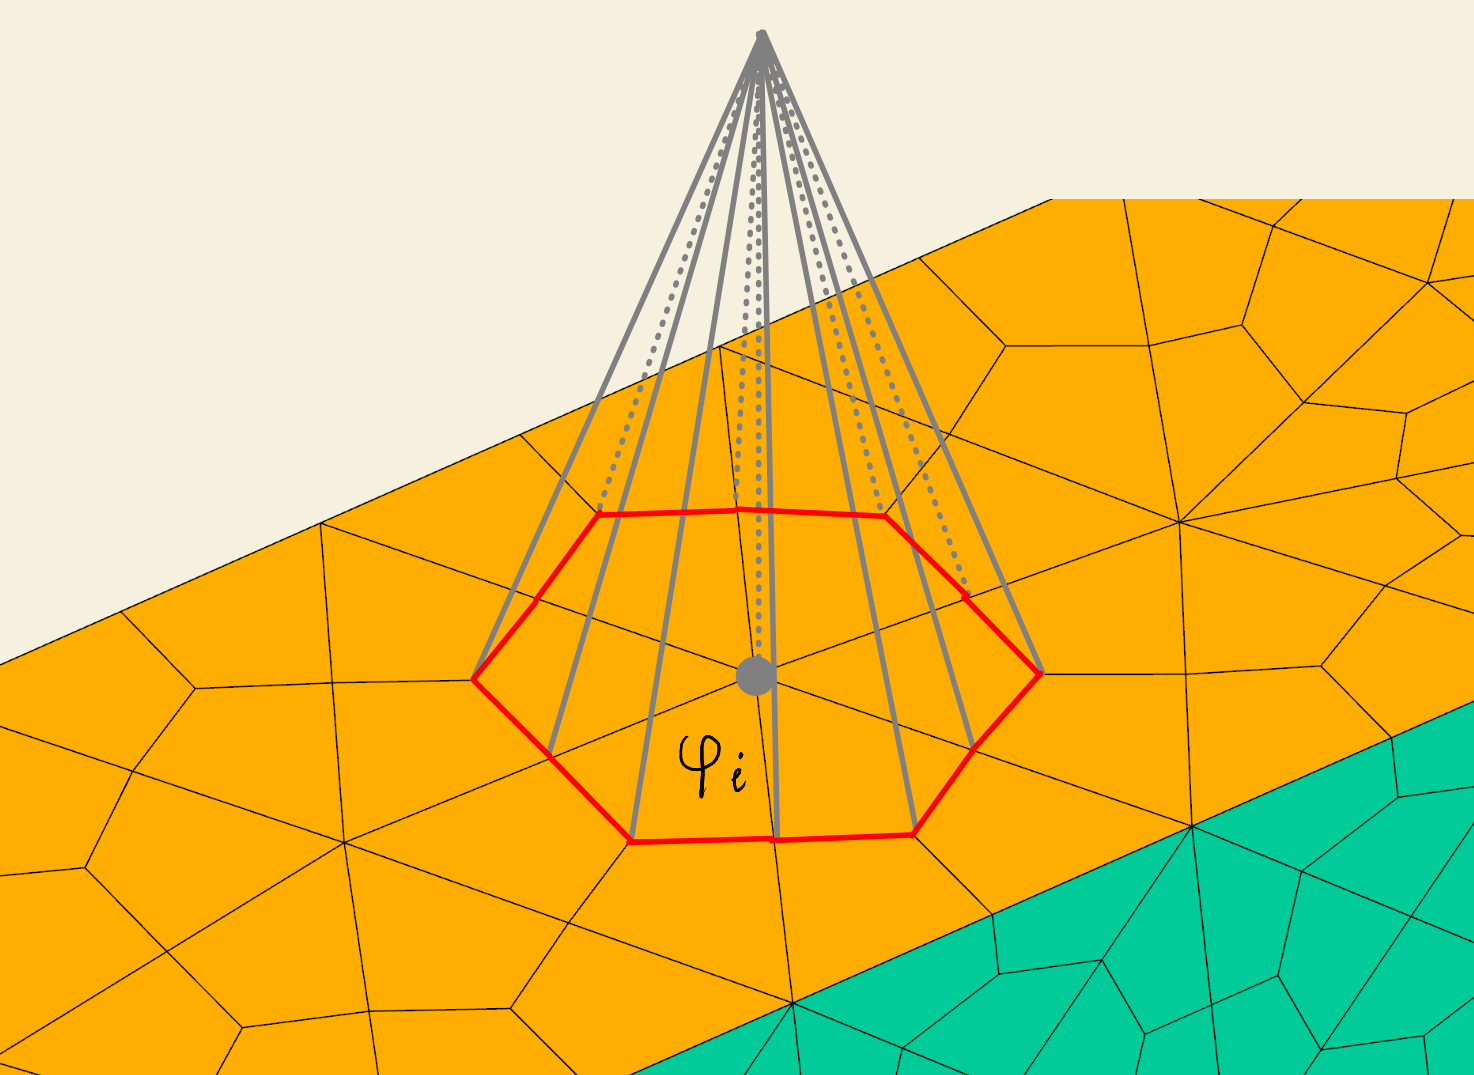
\includegraphics[width=0.5\textwidth, height=\textheight,
  keepaspectratio]{figures/basis-function-with-compact-support-on-mesh-draft}
  \caption{}
  \label{fig:basis-function-with-compact-support}
\end{figure}
Taking Lagrange finite element \texttt{FE\_Q} as example, the construction of a basis
function needs the following steps:
\begin{enumerate}
\item Define a bunch of polynomials $\left\{ \hat{P}_k(\hat{x}) \right\}_{k=1}^N$ on a
  standard cell $\hat{\tau}=[0,1]^2$. $\hat{\tau}$ is called the reference cell and the
  polynomials are called shape functions. Each shape function $\hat{P}_k$ is associated
  with a support point $\hat{p}_k$ in the reference cell, at which $\hat{P}_k$ is
  evaluated to 1. At the support points of the other shape functions, $\hat{P}_k$ is zero,
  i.e. $\hat{P}_k(\hat{p}_{l}) = \delta_k^l$.
\item For each real cell $\tau$ in the mesh, there is a map
  $\chi_{\tau}: \hat{\tau} \rightarrow \tau$ and its inverse
  $\chi_{\tau}^{-1}: \tau \rightarrow \hat{\tau}$. Therefore, the shape functions
  transformed onto the real cell $\tau$ are
  $P_k^{\tau}(x) = \hat{P}_k(\chi_{\tau}^{-1}(x))$, which is the composition of
  $\hat{P}_k$ and $\chi_{\tau}^{-1}$.
\item The basis function $\varphi_i$ is also associated with a support point $p_i$ in the
  real mesh. $p_i$ is usually shared by several neighboring cells
  $\left\{ \tau_{i_{e}} \right\}_{e=1}^{E(i)}$, where $i_e$ is the global cell index of
  the $e$-th cell which contains $p_i$ and $E(i)$ is the total number of cells containing
  $p_i$. For any of these cells $\tau_{i_e}$, there is a support point $\hat{p}_k$ and
  associated shape function $\hat{P}_k$ in its reference cell, such that
  $\chi_{\tau_{i_e}}(\hat{p}_k) = p_i$. N.B. For a different $\tau_{i_e}$ which contains
  $p_i$, the shape function index $k$ in $\hat{P}_k$ is usually different and we can
  define a function $k(i, e)$ which returns this shape function index. The counterpart
  polynomial of $\hat{P}_{k(i_e)}$ in the real cell $\tau_{i_e}$ is
  $P_{k(i, e)}^{\tau_{i_e}}$. Then the basis function $\varphi_i$ is a piecewise
  combination of all such shape functions in the real cells
  $\left\{ \tau_{i_e} \right\}_{e=1}^{E(i)}$:
  \begin{equation}
    \label{eq:basis-function-from-shape-functions}
    \varphi_i(x) = P_{k(i,e)}^{\tau_{i_e}}(x) = \hat{P}_{k(i,e)}\tau_{i_e}^{-1}(x) \quad x\in\tau_{i_e}, e=1,\cdots,E(i).
  \end{equation}
\end{enumerate}

Second order Lagrange shape functions on the reference cell are shown in Figure \ref{fig:lagrange-shape-functions}.
\begin{figure}[htbp]
  \centering
  
\includegraphics[width=0.3\textwidth, height=\textheight,
  keepaspectratio]{figures/n=2_k=(0,0)}
  
\includegraphics[width=0.3\textwidth, height=\textheight,
  keepaspectratio]{figures/n=2_k=(0,1)}
  
\includegraphics[width=0.3\textwidth, height=\textheight,
  keepaspectratio]{figures/n=2_k=(0,2)}
  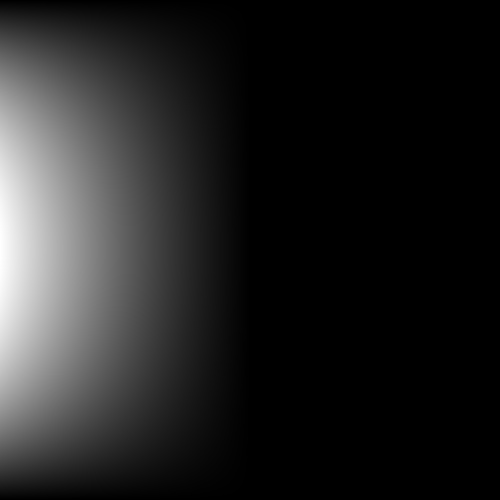
\includegraphics[width=0.3\textwidth, height=\textheight,
  keepaspectratio]{figures/n=2_k=(1,0)}
  
\includegraphics[width=0.3\textwidth, height=\textheight,
  keepaspectratio]{figures/n=2_k=(1,1)}
  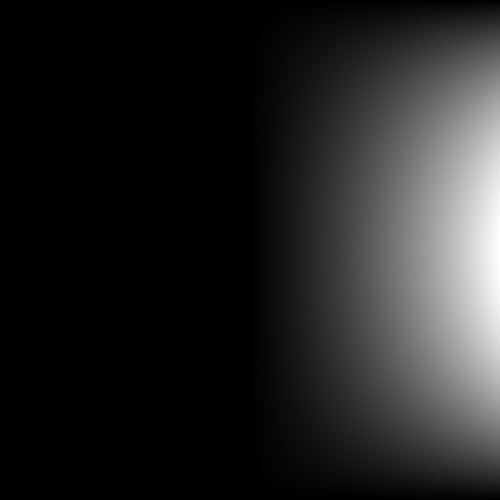
\includegraphics[width=0.3\textwidth, height=\textheight,
  keepaspectratio]{figures/n=2_k=(1,2)}
  
\includegraphics[width=0.3\textwidth, height=\textheight,
  keepaspectratio]{figures/n=2_k=(2,0)}
  
\includegraphics[width=0.3\textwidth, height=\textheight,
  keepaspectratio]{figures/n=2_k=(2,1)}
  
\includegraphics[width=0.3\textwidth, height=\textheight,
  keepaspectratio]{figures/n=2_k=(2,2)}
  \caption{}
  \label{fig:lagrange-shape-functions}
\end{figure}

Figure \ref{fig:local-shape-function-and-global-dof} shows the numbering of vertices and
cells in the mesh, local shape function indices in each cell, shape function indices
related to the global basis function or DoF with the index 10. N.B. The shape functions in
each cell are in the lexicographic order and the first shape function starts from the
first vertex in the cell.
\begin{figure}[htbp]
  \centering
  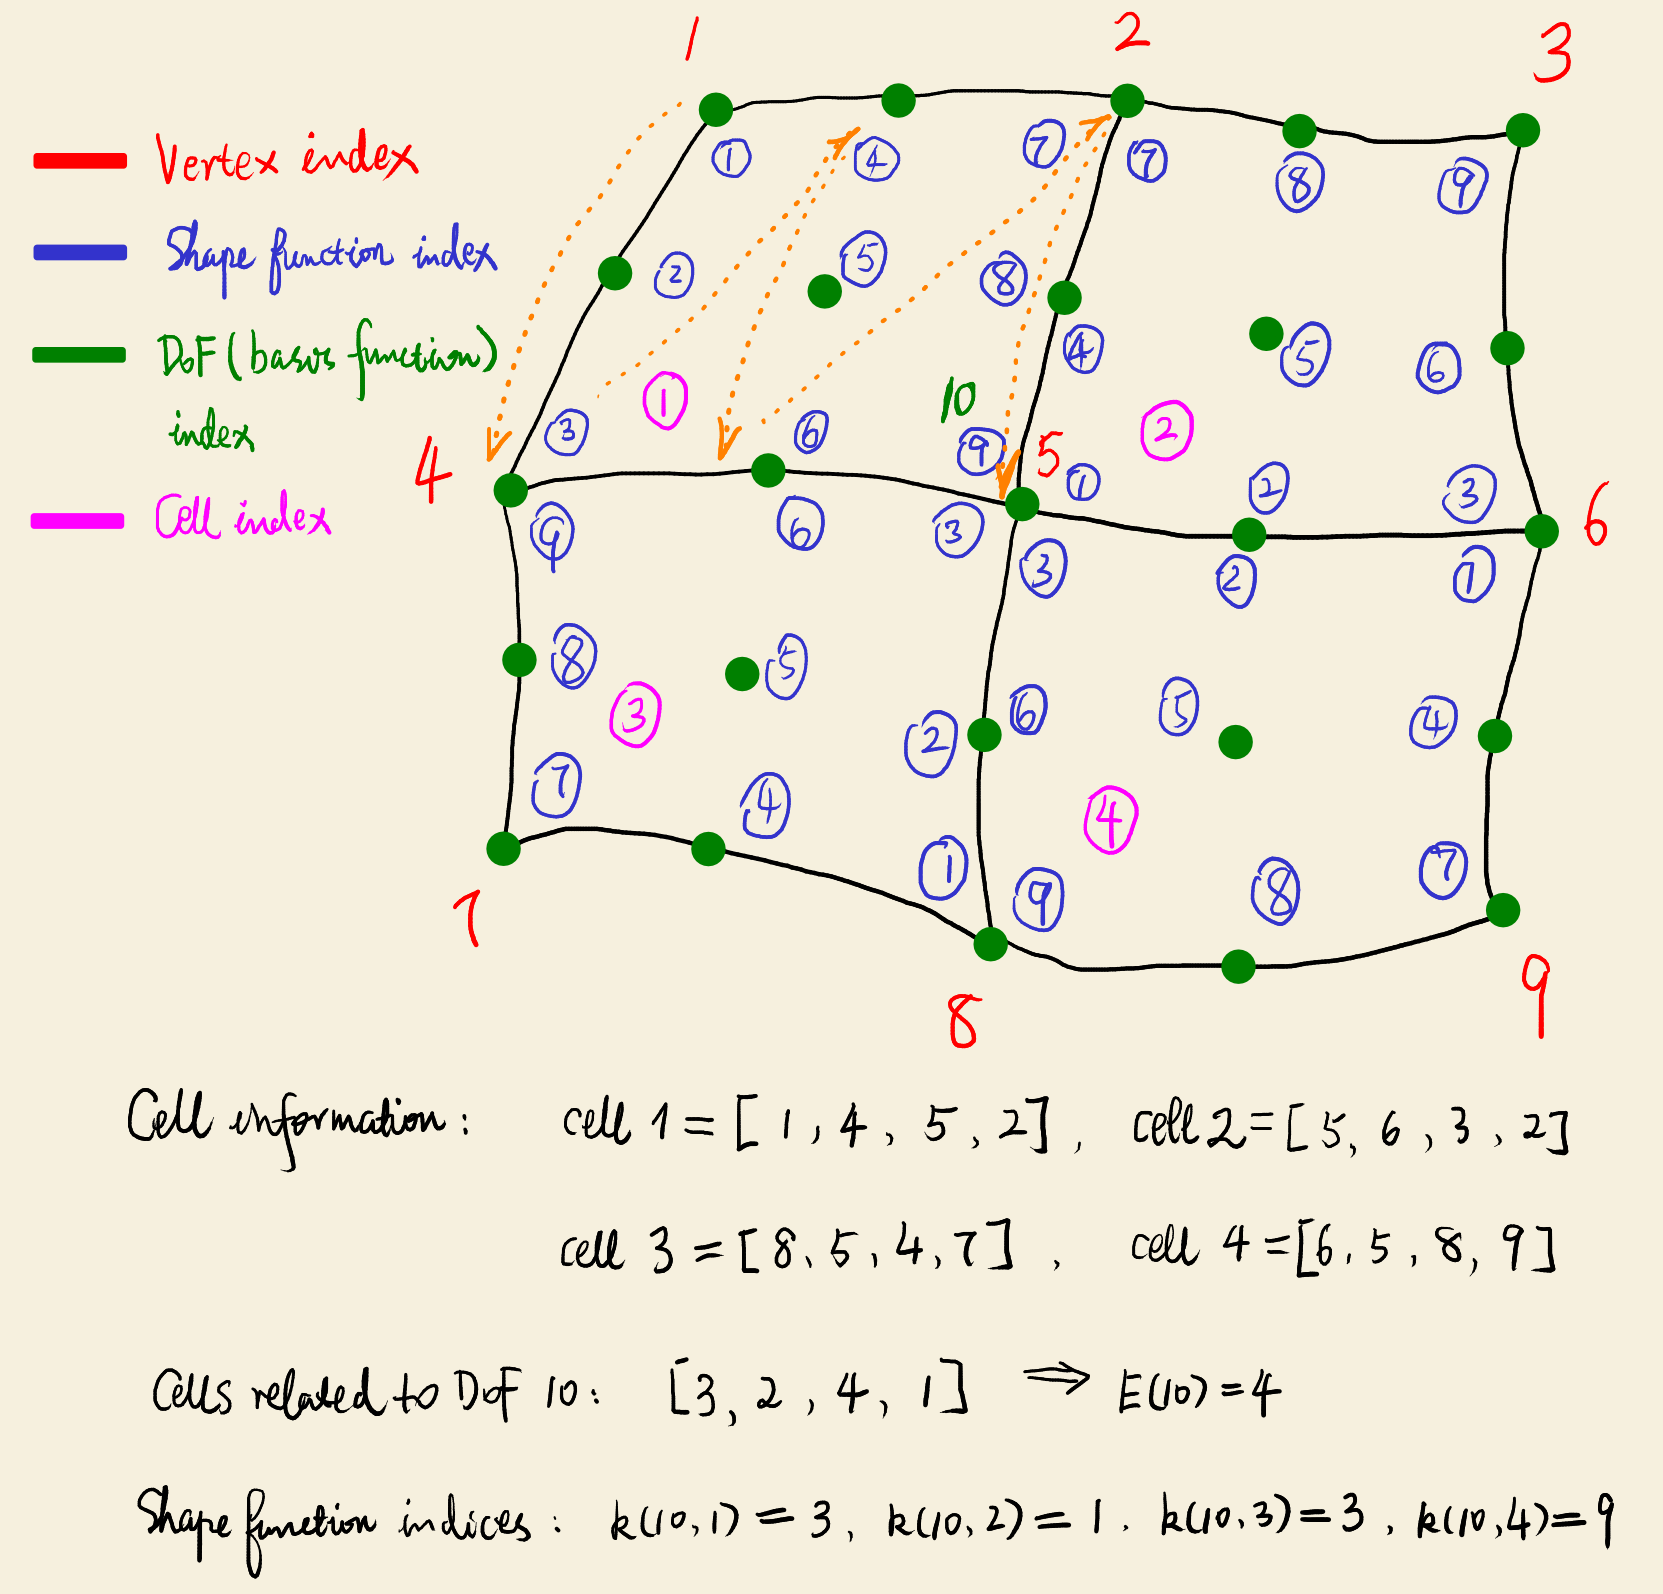
\includegraphics[width=0.7\textwidth, height=\textheight, keepaspectratio]{figures/shape-function-index-and-global-dof-index-draft}
  \caption{}
  \label{fig:local-shape-function-and-global-dof}
\end{figure}
If the finite element \texttt{FE\_DGQ} is adopted, because it is a discontinuous element,
the situation is much simpler. According to Figure \ref{fig:fe-dgq-2nd-order}, on the
common edge between the two cells, there are duplicated support points. Take the central
point on the edge as example, the \texttt{DoFHandler} will assign two basis functions for
it: $\varphi_i$ for the left cell and $\varphi_{i'}$ for the right cell. Then each basis
function belongs to only one cell and it relates to only one shape function in the
associated reference cell. Therefore, there is no need to find all
cells sharing a common support point as what is done for \texttt{FE\_Q}.
\begin{figure}[htbp]
  \centering
  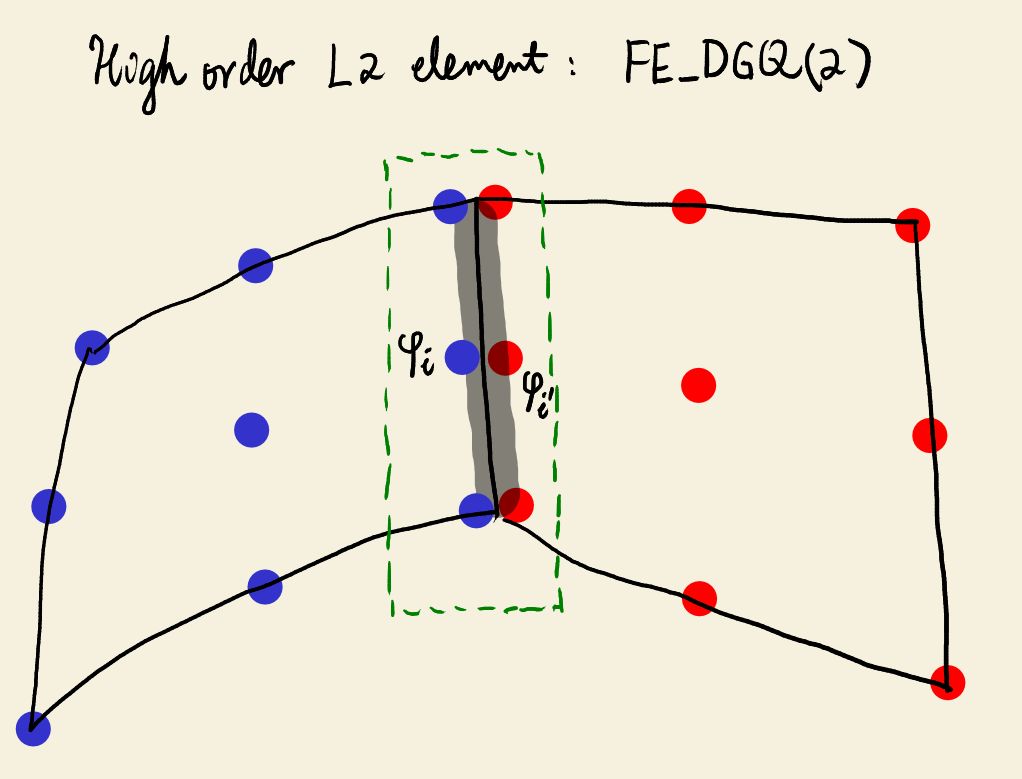
\includegraphics[width=0.5\textwidth, height=\textheight, keepaspectratio]{figures/fe-dgq-2nd-order}
  \caption{}
  \label{fig:fe-dgq-2nd-order}
\end{figure}

When basis functions with compact support are adopted for test and ansatz spaces, the
integration domain will be restricted to only a few cells. If \texttt{FE\_Q} is adopted,
computation of the matrix entry $\mathscr{A}_{ij}$ in
\eqref{eq:bilinear-form-matrix-entry} now becomes
\begin{equation}
  \label{eq:bilinear-form-matrix-entry-cell-pairs}
  \begin{aligned}
    \mathscr{A}_{ij} &= \int_{\left\{ \tau_{i_{e}} \right\}_{e=1}^{E(i)}} \psi_i(x)
    \int_{\left\{ \tau_{j_{e'}} \right\}_{e'=1}^{E(j)}} k(x,y)\varphi_j(y) \intd s_y \intd
    s_x \\
    &= \sum_{e=1}^{E(i)} \sum_{e'=1}^{E(j)} \int_{\tau_{i_e}} \psi_i(x)
  \int_{\tau_{j_{e'}}} k(x,y)\varphi_j(y) \intd s_y \intd s_x \\
    &= \sum_{e=1}^{E(i)} \sum_{e'=1}^{E(j)} \int_{\tau_{i_e}} P_{k(i,e)}^{\tau_{i_e}}(x)
  \int_{\tau_{j_{e'}}} k(x,y) P_{k(j,e')}^{\tau_{j_e}}(y) \intd s_y \intd s_x.
  \end{aligned}
\end{equation}
This indicates that an entry $\mathscr{A}_{ij}$ in the matrix of a bilinear form is
contributed from the interaction of a shape function within each cell in the support of
$\psi_i(x)$ and a shape function within each cell in the support of $\varphi_j(y)$.
Therefore, a double loop is needed to compute $\mathscr{A}_{ij}$.

If \texttt{FE\_DGQ} is adopted for both ansatz and test spaces, each basis function or DoF
belongs to only one cell and Equation \eqref{eq:bilinear-form-matrix-entry-cell-pairs} has a
simpler form
\begin{equation}
  \label{eq:bilinear-form-matrix-entry-cell-pairs-fedgq}
  \mathscr{A}_{ij} = \int_{\tau_i} P_{k(i)}^{\tau_i}(x)
  \int_{\tau_j} k(x,y) P_{k(j)}^{\tau_j}(y) \intd s_y \intd s_x.
\end{equation}
The $i$-th basis function in the test space belongs to the cell $\tau_i$ and the $j$-th
basis function in the ansatz space belongs to the cell $\tau_j$. The index of the
corresponding shape function in $\tau_i$ is $k(i)$, which only depends on the DoF index
$i$. Similarly, the index of the corresponding shape function in $\tau_j$ is $k(j)$.
Therefore, in this case, $\mathscr{A}_{ij}$ can be directly computed without the double
loop for \texttt{FE\_Q}.

\section{Surface integral in 3D space}

Let $S$ be a surface in the 3D space $\mathbb{R}^3$. Since $S$ is intrinsically a 2D
object (it may be curved), it can be characterized with only two coordinate variables.
Even though $S$ may not be represented in a unique \emph{global} 2D coordinate frame, $S$
can be partitioned into a collection of subdomains, each of which can be assigned a
\emph{local} 2D coordinate frame or chart. When any two of the charts have an overlap, any
point in their intersection should have consistent coordinates when its coordinates in two
local frames are transformed into the global frame. Meanwhile, the transformations between
these local 2D frames are differentiable. The set of all these local frames forms a
complete representation of the whole surface $S$, which is called \emph{atlas}. Then $S$
is called a 2D \emph{differential manifold} embedded in $\mathbb{R}^3$ and $\mathbb{R}^3$
is the ambient space of $S$. These are basic concepts in differential geometry.
\begin{figure}[htbp]
  \centering
  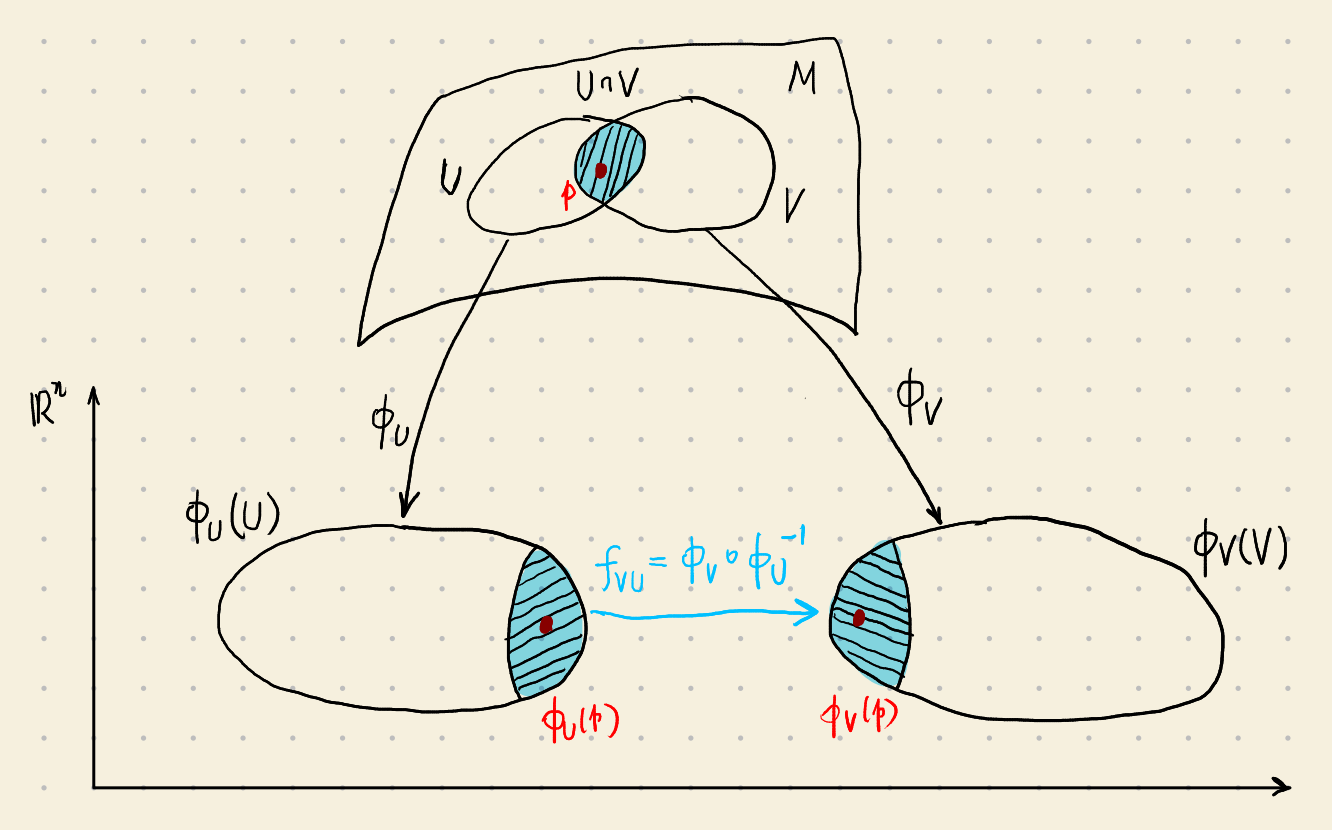
\includegraphics[width=0.5\textwidth, height=\textheight, keepaspectratio]{figures/manifold-draft}
  \caption{}
  \label{fig:differential-manifold}
\end{figure}
A typical example of a 2D differential manifold is the sphere. As shown in Figure
\ref{fig:sphere-manifold}, six open sets on the sphere can be assigned their individual
local coordinate frames.
\begin{figure}[htbp]
  \centering
  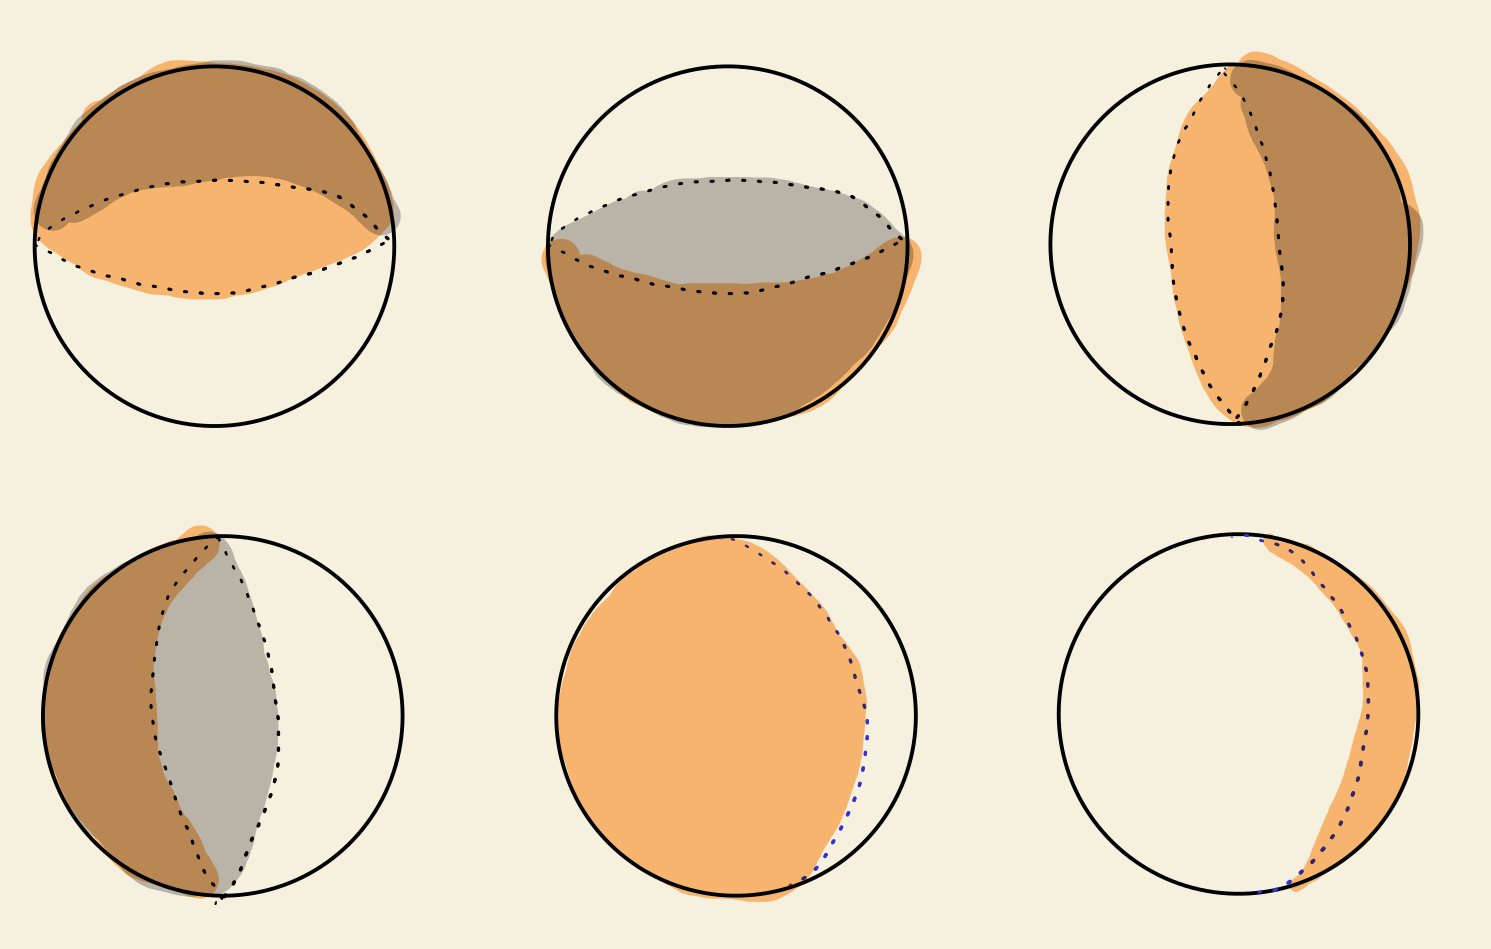
\includegraphics[width=0.5\textwidth, height=\textheight, keepaspectratio]{figures/coordinate-chart-for-sphere-draft}
  \caption{}
  \label{fig:sphere-manifold}
\end{figure}
In FEM or BEM, the geometric model for simulation is built in the ambient space
$\mathbb{R}^3$. Then we discretize the geometric domain into a triangulation
$\mathcal{T}$, construct finite element basis functions directly on the reference cell
$\hat{\tau}$ and maintain a set of maps
$\left\{ \chi_{\tau} \right\}_{\tau\in\mathcal{T}}$ from the reference to cell
$\hat{\tau}$ to each real cell $\tau$ in the triangulation $\mathcal{T}$ (see Figure
\ref{fig:mesh-manifold}). This process is equivalent to creating an atlas, in which each
coordinate chart is local to each cell. We can say FEM or BEM itself is an direct
embodiment of the spirit of differential geometry.
\begin{figure}[htbp]
  \centering
  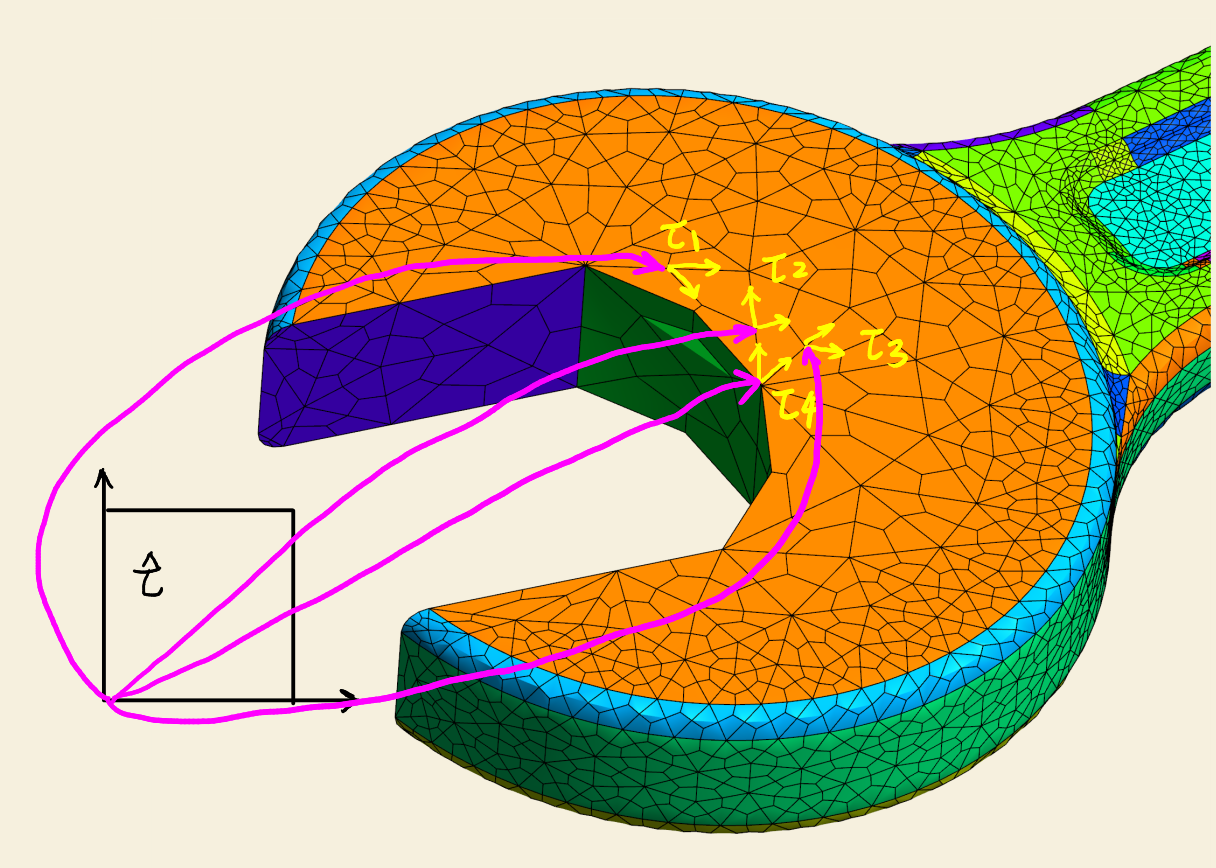
\includegraphics[width=0.5\textwidth, height=\textheight, keepaspectratio]{figures/coordinate-chart-for-mesh-draft}
  \caption{}
  \label{fig:mesh-manifold}
\end{figure}

Let $\mathbb{R}^3$ be parameterized by $(x_1,x_2,x_3)$. Let the integration domain
$\Gamma$ in Equation \eqref{eq:bilinear-form-matrix-entry} be locally parameterized by
$(\hat{x}_1,\hat{x}_2)$, i.e. in each cell $\tau$ in $\Gamma$, the coordinate frame of its
reference cell is adopted. Because double integral is involved, for each pair of cells,
the actual integration domain is a 4D hyper-cube $[0,1]^4$. Because both shape functions
and quadrature points are defined on reference cells, it is easy do calculus in reference
cells.

When a coordinate transformation is applied to a surface integral, a scaling of the
integral element $\partial \hat{x}_1 \wedge \partial \hat{x}_2$ is needed. On a curved
surface or 2D manifold, such scaling is the area of the parallelogram spanned by the
tangent vectors $\frac{\pdiff x}{\pdiff \hat{x}_1}$ and
$\frac{\pdiff x}{\pdiff \hat{x}_2}$ (see Figure \ref{fig:surface-element-scaling}).
\footnote{In a cell $\tau$, the transformation from $(\hat{x}_1, \hat{x}_2)$ to $x$ is
  just $\chi_{\tau}$.}
\begin{figure}[htbp]
  \centering
  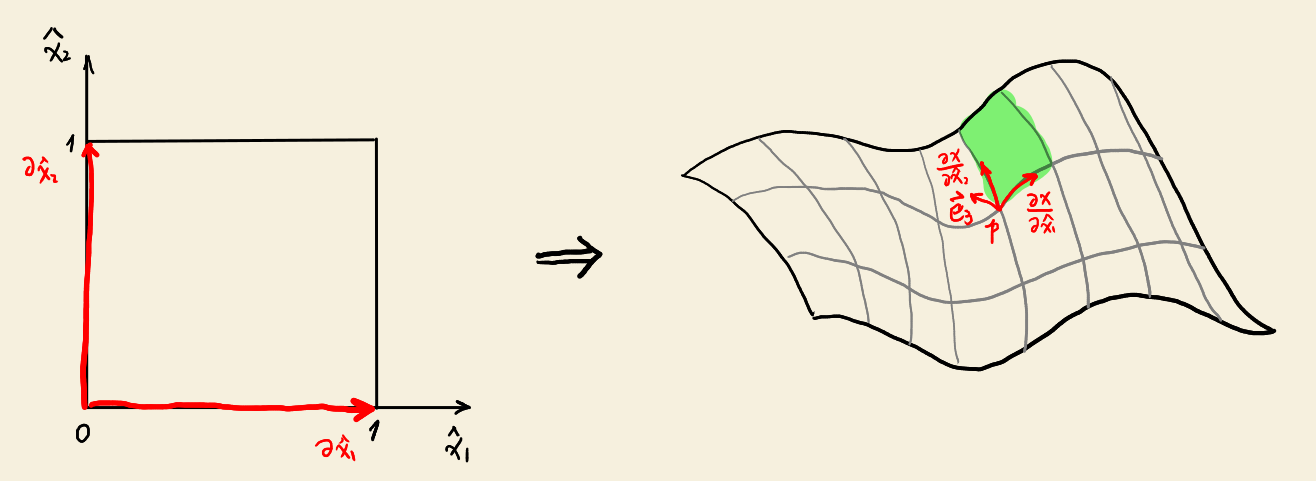
\includegraphics[width=0.5\textwidth, height=\textheight, keepaspectratio]{figures/surface-element-scaling-draft}
  \caption{}
  \label{fig:surface-element-scaling}
\end{figure}
The scaling factor is equal to the amplitude of the cross product of the two tangent
vectors:
\begin{equation}
  \tilde{\vect{e}}_3=\tilde{\vect{e}}_1\times\tilde{\vect{e}}_2=\left\vert\begin{matrix}
      \vect{i} & \vect{j} & \vect{k} \\
      \frac{\pdiff x_{1}}{\pdiff \hat{x}_{1}} & \frac{\pdiff x_{2}}{\pdiff \hat{x}_{1}} & \frac{\pdiff
        x_{3}}{\pdiff \hat{x}_{1}} \\
      \frac{\pdiff x_{1}}{\pdiff \hat{x}_{2}} & \frac{\pdiff x_{2}}{\pdiff \hat{x}_{2}} & \frac{\pdiff
        x_{3}}{\pdiff \hat{x}_{2}}
    \end{matrix}\right\vert=
  \left\vert\frac{\pdiff (x_{2},x_{3})}{\pdiff (\hat{x}_1,\hat{x}_2)}\right\vert \vect{i} +
  \left\vert\frac{\pdiff (x_{3},x_{1})}{\pdiff (\hat{x}_1,\hat{x}_2)}\right\vert \vect{j} +
  \left\vert\frac{\pdiff (x_{1},x_{2})}{\pdiff (\hat{x}_1,\hat{x}_2)}\right\vert \vect{k}
\end{equation}

\begin{mycomment}
  Note the order of the subscripts: $(2,3)$, $(3,1)$, $(1,2)$. If the subscript starts from 0, we
  have $(1,2)$, $(2,0)$, $(0,1)$. Such cyclic indices are similar to those appearing in the $\curl$
  operation, for example,
  \begin{equation}
    \curl\vect{A} =
    \left\vert\begin{matrix}
        \vect{i} & \vect{j} & \vect{k} \\
        \frac{\pdiff }{\pdiff x_1} & \frac{\pdiff }{\pdiff x_2} & \frac{\pdiff }{\pdiff x_3} \\
        A_1 & A_2 & A_3
    \end{matrix}\right\vert = \left( \frac{\pdiff A_3}{\pdiff x_{\emphr{2}}} - \frac{\pdiff A_{2}}{\pdiff
      x_{\emphr{3}}} \right) \vect{i} + \left( \frac{\pdiff A_{1}}{\pdiff x_{\emphr{3}}} -
    \frac{\pdiff A_{3}}{\pdiff x_{\emphr{1}}} \right) \vect{j} + \left( \frac{\pdiff A_{2}}{\pdiff
      x_{\emphr{1}}} - \frac{\pdiff A_{1}}{\pdiff x_{\emphr{2}}} \right) \vect{k}.
  \end{equation}
  The cyclic indices can be generated by using the $\mod$ operation as below.
  \begin{enumerate}
  \item When the index starts from 0:
    \begin{breakablealgorithm}
      \caption{Generate curl-like pairs of cyclic indices ($starting\_index \equiv 0$)}
      \begin{algorithmic}[1]
        \For {$i=[0,1,2]$}
          \State {(i\%3, (i+1)\%3)}
        \EndFor
      \end{algorithmic}
    \end{breakablealgorithm}
    It produces the index pairs $(0,1), (1,2), (2,0)$.
  \item When the index starts from 1:
    \begin{breakablealgorithm}
      \caption{Generate curl-like pairs of cyclic indices ($starting\_index \equiv 1$)}
      \begin{algorithmic}[1]
        \For {$i=[1,2,3]$}
          \State {$([(i-1)\%3]+1, i\%3+1)$}
        \EndFor
      \end{algorithmic}
    \end{breakablealgorithm}
    It produces the index pairs $(1,2),(2,3),(3,1)$.
  \end{enumerate}

  \alertbox{It can be seen that using indices starting from zero is more convenient than
    starting from 1.}
\end{mycomment}

Let $\abs{J_{23}} = \left\vert \frac{\pdiff (x_2,x_3)}{\pdiff (\hat{x}_1,\hat{x}_2)}\right\vert$,
$\abs{J_{31}} = \left\vert \frac{\pdiff (x_3,x_1)}{\pdiff (\hat{x}_1,\hat{x}_2)}\right\vert$ and
$\abs{J_{12}} = \left\vert \frac{\pdiff (x_1,x_2)}{\pdiff (\hat{x}_1,\hat{x}_2)}\right\vert$. Then
the unit normal vector at $(\hat{x}_1,\hat{x}_2)$ is
\begin{equation}
  \label{eq:surface-normal-vector}
  \vect{n} = \frac{(\abs{J_{23}},\abs{J_{31}},\abs{J_{12}})^T}{(\abs{J_{23}}^2+\abs{J_{31}}^2+\abs{J_{12}}^2)^{\frac{1}{2}}}.
\end{equation}
The scaling factor or surface metric is
\begin{equation}
  \label{eq:surface-metric}
  \abs{J} = (\abs{J_{23}}^2+\abs{J_{31}}^2+\abs{J_{12}}^2)^{\frac{1}{2}}.
\end{equation}

$\abs{J}$ can also be calculated from the Gramian matrix $G = J^TJ$, with $J$ being the
Jacobi matrix of the map from unit cell to real cell:
\begin{equation}
  \label{eq:surface-metric-from-gramian-matrix}
  \abs{J} = \sqrt{\det(G)} = \sqrt{\det(J^TJ)}.
\end{equation}
The covariant matrix $C$ can also be calculated from $G$, which will be used for
coordinate transformation of gradient vector:
\begin{equation}
  \label{eq:covariant-matrix}
  C = J G^{-1} = J(J^TJ)^{-1}.
\end{equation}

In a cell $K^e$, let the number of DoFs for geometry representation be $n$. The coordinate
components of $x\in K^e$ are the linear combination of shape functions:
\begin{equation}
  \begin{split}
    x &= \sum_{i=1}^n x_iN_i(\xi_1,\xi_2) \\
    y &= \sum_{i=1}^n y_iN_i(\xi_1,\xi_2) \\
    z &= \sum_{i=1}^n z_iN_i(\xi_1,\xi_2)
  \end{split}
\end{equation}

General form of the integrals to be handled in BEM:
\begin{equation}
  \int_{\Gamma} \varphi_i(x) \int_{\Gamma}k(x,y,y-x) \varphi_j(y) \intd s_y \intd s_x
\end{equation}
\begin{equation}
  \int_{\Gamma}\varphi_i(x)\int_{\Gamma}k(x,y,y-x)r(y) \intd s_y \intd s_x
\end{equation}
where $r(y)$ is a given function on the right-hand side. If $r(y)$ is expanded by the basis
functions $\{\varphi_j(y)\}_{j\geq 1}$, this second integral is the same as the first one.

For integration over pairs of panels $\tau\times t$, there are four cases to be handled:
\begin{enumerate}
\item Identical panels
\item Common edge
\item Common vertex
\item Regular
\end{enumerate}

\section{Cell mapping}

As said above, the map from a reference cell to a real cell is $\chi_{\tau}: \hat{\tau}
\rightarrow \tau$. Moreover, in Sauter quadrature, 


\section{Detection of cell neighboring types}

\begin{itemize}
\item 
\end{itemize}

\section{Ordering of support points}

Assume there is a 4x4 grid assigned with the two kinds of numbering, lexicographic and hierarchic. Use the grid point as the physical entity for establishing an equivalence or mapping relation between the two types of numbering.

Under this notion, the function \texttt{FETools::lexicographic\_to\_hierarchic\_numbering} returns an array of indices in the hierarchic numbering, which corresponds to the list of lexicographic numbering in the natural order \(0,1,\cdots,15\). The array is
\begin{lstlisting}[language=text]
[0,8,9,1,4,12,13,6,5,14,15,7,2,10,11,3]
\end{lstlisting}

which can be considered as the mapping from lexicographic numbering to hierarchic numbering, or as the assignment of the hierarchic numbering to the lexicographic numbering.

On the contrary, the function \texttt{FETools:hiergraphic\_to\_lexicographic\_numbering}
returns an array of indices in the lexicographic numbering, which corresponds to the list
of hierarchic numbering in the natural order \(0,1,\cdots,15\). The array is
\begin{lstlisting}[language=text]
[0,3,12,15,4,8,7,11,1,2,13,14,5,6,9,10]
\end{lstlisting}

Another understanding is like this. For \texttt{FETools::lexicographic\_to\_hierarchic\_numbering}, it is equivalent to think a list of naturally ordered numbering \(0,1,\cdots,15\) arranged in the space in the hierarchic order, which is to be accessed in the lexicographic order. Similarly, for \texttt{FETools::hierarchic\_to\_lexicographic\_numbering}, it is a list of naturally ordered numbering arranged in the space int he lexicographic order, which is to be accessed in the hierarchic order.

Generally, assume there are two sets of numbering \(A\) and \(B\) assigned to a same grid. A direct index mapping from \(A\) to \(B\) is used to access in the order \(A\) a naturally ordered numbering, which is arranged in the space in the order \(B\).

\begin{figure}[htbp]
\centering
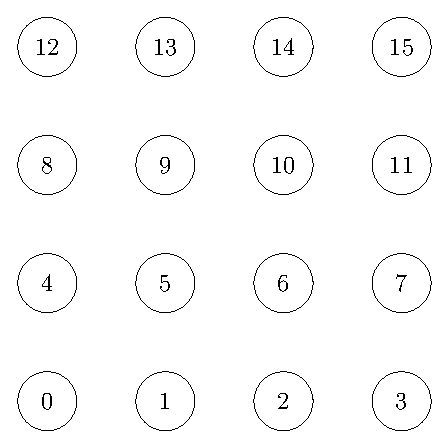
\includegraphics[width=0.3\textwidth]{figures/2022-05-25-lexicographic-numbering.eps}
\caption{Lexicographic numbering assigned to a 4x4 gird.}
\end{figure}

\begin{figure}[htbp]
\centering
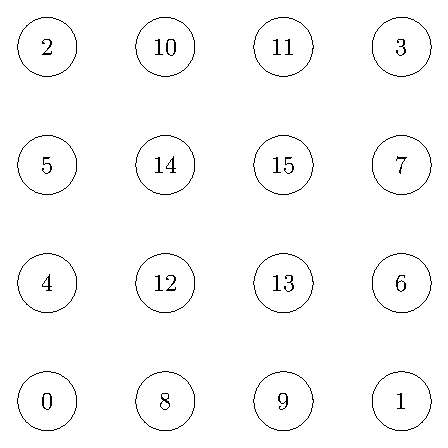
\includegraphics[width=0.3\textwidth]{figures/2022-05-25-hierarchic-numbering.eps}
\caption{Hierarchic numbering assigned to a 4x4 grid.}
\end{figure}

\section{Reason for making local copies of mapping objects in
  \texttt{sauter\_assemble\_on\_one\_pair\_of\_dofs} and
  \texttt{sauter\_assemble\_on\_one\_pair\_of\_cells}}

At the moment, in the \texttt{LaplaceBEM} class, there are only two mapping objects \texttt{kx\_mapping} and \texttt{ky\_mapping} of the type \texttt{MappingQGenericExt} defined. When calling the member function \texttt{MappingQGenericExt::compute\_mapping\_support\_points}, the member variable \texttt{support\_points} in \texttt{MappingQGenericExt} will be overwritten.

\begin{enumerate}
\item \texttt{sauter\_assemble\_on\_one\_pair\_of\_cells} is called by \texttt{assemble\_bem\_full\_matrix}. In this function, the outer loop iterates over each cell in the test space, while the TBB parallelized inner loop iterates over each cell in the trial space. In the outer loop, the mapping support points and DoF indices are computed for \(K_x\) in the main thread without parallelism. In the inner loop, several working threads need to calculate the mapping support points and DoF indices for their own \(K_y\) in parallel. Hence, if these threads operates directly on only one instance of \texttt{ky\_mapping}, there will be resource competition and memory inconsistency.

Therefore, the current solution is to pass \texttt{kx\_mapping} and \texttt{ky\_mapping} into \texttt{sauter\_assemble\_on\_one\_pair\_of\_cells} via \texttt{const} references. Inside this function, a local copy associated with the thread is made for \texttt{ky\_mapping} for calculating the mapping support points and DoF indices. Since \texttt{kx\_mapping} related data have already been computed in the outer loop in \texttt{assemble\_bem\_full\_matrix}, there is no need to recalculate it in \texttt{sauter\_assemble\_on\_one\_pair\_of\_cells}.

\item \texttt{sauter\_assemble\_on\_one\_pair\_of\_dofs} is called by \texttt{fill\_hmatrix\_leaf\_node\_with\_aca\_plus}, which itself contains double loops, with the outer loop iterating over the cells in the support of the \(i\)-th DoF and the inner loop iterating over the cells in the support of the \(j\)-th DoF. Because \texttt{fill\_hmatrix\_leaf\_node\_with\_aca\_plus} will be executed in several TBB threads at the same time, computation of the mapping support points should be performed in thread dependent local copies of \texttt{kx\_mapping} and \texttt{ky\_mapping}. Similar to the treatment in \texttt{sauter\_assemble\_on\_one\_pair\_of\_cells}, \texttt{kx\_mapping} and \texttt{ky\_mapping} are passed as const references into \texttt{sauter\_assemble\_on\_one\_pair\_of\_dofs}. Inside this function, a local copy of \texttt{kx\_mapping} is made in the outer loop and another copy of \texttt{ky\_mapping} is made in the inner loop.
\end{enumerate}

\section{Identical panels}

The integral is performed in the sense of Cauchy principal value:
\begin{equation}
  \int_{\tau} \varphi_i(x) \; p.v.\int_{\tau}k(x,y,y-x) \varphi_j(y) \intd s_y \intd s_x
\end{equation}

Merge the basis function $\varphi_i$ and $\varphi_j$ into the kernel, we define
$k_1(x,y,z)=\varphi_i(x)k(x,y,z)\varphi_j(y)$. For $x\in\tau$ and sufficiently small
$\varepsilon_0>0$, define
\begin{equation}
  I_{\varepsilon}\coloneqq \int_{\tau}\int_{\tau\backslash B_{\varepsilon}(x)} k_1(x,y,y-x) \intd
  s_y \intd s_x
\end{equation}

Let $\chi_{\tau}: \hat{\tau} \rightarrow \tau$ be the map from the reference cell to the real cell
$\tau$. Then pull back the function $k_1$ from the real cell to the reference cell, define the
function $k_2$:
\begin{equation}
  k_2(\hat{x}, \hat{y}) \coloneqq k_1(\chi_{\tau}(\hat{x}), \chi_{\tau}(\hat{y}), \chi_{\tau}(\hat{y})
  - \chi_{\tau}(\hat{x})) g_{\tau}(\hat{x}) g_{\tau}(\hat{y})
\end{equation}
where $g_{\tau}(\hat{x})$ is the Jacobian determinant of the map $\chi_{\tau}$ which is evaluated at
$\hat{x}$.

\section{Common edge}

\subsection{Permutation of the support points and DoF indices}

\draft{About finding the starting vertex}

Assume the list of support points are arranged the lexicographic or reversed lexicographic order.
Extract those support points located at cell vertices. Then if we swap the last two vertex support
points, the list of vertex support points will be in either clockwise or counter-clockwise order.

\draft{General work flow}

This part handles the common edge case of Sauter's quadrature rule.
\begin{enumerate}
\item Get the DoF indices in the lexicographic order for $K_x$.
\item Get the DoF indices in the reversed lexicographic order for $K_y$.
\item Extract only those DoF indices which are located at cell vertices in $K_x$ and $K_y$.
  N.B. The DoF indices for the last two vertices are swapped, such that the four vertices are in
  either clockwise or counter clockwise order.
\item Determine the starting vertex for $K_x$ and regenerate the permutation numbering for
  traversing in the forward lexicographic order by starting from this vertex.
\item Determine the starting vertex for $K_y$ and regenerate the permutation numbering for
  traversing in the backward lexicographic order by starting from this vertex.
\item Apply permutation to support points and DoF indices using the newly generated permutation
  numbering schemes.
\end{enumerate}


\section{Common vertex}

\section{General formulation}

The integrand in local coordinates for the reference cell is
\begin{equation}
  k_3(\hat{x}, \hat{y}) \coloneqq \hat{\varphi_i}(\hat{x})\hat{\varphi_j}(\hat{y})
  k(\chi_{\tau}(\hat{x}), \chi_{\tau}(\hat{y}), \chi_{\tau}(\hat{y}) 
  - \chi_{\tau}(\hat{x})) g_{\tau}(\hat{x}) g_{\tau}(\hat{y})
\end{equation}
The integral on pairs of panels is
\begin{equation}
  I_{\tau\times t} \coloneqq \int_{\hat{\tau}} p.v. \int_{\hat{t}} k_3(\hat{x},\hat{y}) \intd
  \hat{y} \intd \hat{x}
\end{equation}
The integral variables $(\hat{x}, \hat{y})$ will further be pulled back to the parameter space.

\section{Cell pair configuration and permutation of DoFs}

\subsection{Common edge case}

\begin{itemize}
\item Because the DoFs in $K_y$ are accessed in the reversed lexicographic order due to permutation,
  the calculated surface normal vector $n_y$ using Equation \eqref{eq:surface-normal-vector} has a
  direction opposite to the real normal vector. Therefore, it should be negated when it is used in
  the kernel function evaluation.
\item Extract the DoFs of the four vertices in $K_x$ and $K_y$ to determine the common edge and the
  starting point. Because the DoFs are accessed in the lexicographic or reversed lexicographic
  order, the vertices corresponding to the obtained four DoFs are in a zigzag form. Therefore, the
  last two elements should be swapped so that the vertices are in the clockwise or counter clockwise
  order.
\end{itemize}

\subsection{Common vertex case}

\section{Precalculation of data tables}

\begin{itemize}
\item Precalculation of data tables is mandatory for achieving a practical performance.
\item It involves different $k_3$ terms in the panel pair integral $I_{\tau\times t}$. This is
  because different $k_3$ terms are pulled back to the parameter space under different mapping
  relations. Therefore, besides the dimensions for shape function index and quadrature point index
  in the table, an additional dimension for indexing $k_3$ terms is required.
\item Table \ref{tab:shape-value-table} shows the dimensions for shape function value.
\item In Table \ref{tab:shape-grad-value-table}, each data item in the table is itself a matrix with
  the dimension $dofs\_per\_cell*spacedim$.
\item Number of shape functions is $(fe\_order+1)^{dim}=(fe\_order+1)^{2}$, since tensor product shape functions
  constructed on the submanifold with dimension $dim$ are adopted.
\item Number of quadrature points is $quad\_order^{2*dim}=quad\_order^{4}$, since the quadrature is
  performed on a \textbf{pair} of unit cells.
\end{itemize}

\begin{table}[tbp]
  \caption{\label{tab:shape-value-table} Data table for shape function values used in Sauter quadrature.}
  \centering
  \begin{tabular}{*{3}{|c}|}\hline
    \textbf{Dimension name} & \multicolumn{2}{|c|}{\textbf{Dimension size}} \\\hline
    Shape function index & \multicolumn{2}{|c|}{$dofs\_per\_cell$} \\\hline
    $k_3$ term index & Same panel & 8 \\\cline{2-3}
                            & Common edge & 6 \\\cline{2-3}
                            & Common vertex & 4 \\\cline{2-3}
                            & Regular & 1 \\\hline
    Quadrature point index & \multicolumn{2}{|c|}{Number of quadrature points} \\\hline
  \end{tabular}
\end{table}

\begin{table}[tbp]
  \caption{\label{tab:shape-grad-value-table} Data table for the gradient of shape functions used in Sauter quadrature.}
  \centering
  \begin{tabular}{*{3}{|c}|}\hline
    \textbf{Dimension name} & \multicolumn{2}{|c|}{\textbf{Dimension size}} \\\hline
    $k_3$ term index & Same panel & 8 \\\cline{2-3}
                            & Common edge & 6 \\\cline{2-3}
                            & Common vertex & 4 \\\cline{2-3}
                            & Regular & 1 \\\hline
    Quadrature point index & \multicolumn{2}{|c|}{Number of quadrature points} \\\hline
  \end{tabular}
\end{table}

\section{Design of data organization for parallelization}

\begin{itemize}
\item The definition of the class \texttt{BEMValues} is a counterpart of the \texttt{FEValues}
  defined in deal.ii.
\item \texttt{BEMValues} are not reinitialized for each pair of cells, because its data,
  i.e. shape function values and their gradient values\footnote{At the moment, only first
    order derivatives are computed and stored.} (with respect to the local
  coordinates) as well as Sauter's quadrature rules are all defined or evaluated on the
  unit cell, which do not depend on the information of the real cells.
\item \emph{Purpose of \texttt{ScratchData}: all large chunks of data involving dynamic memory
    allocation during the computation of cell or pair cell integral should be encapsulated into
    \texttt{ScratchData}. Before the quadrature computation on each pair of cells,
    \texttt{ScratchData} should be reinitialized.}
\item \emph{Purpose of \texttt{PerTaskData}: all large chunks of data involving dynamic memory
    allocation during the \texttt{copy\_local\_to\_global} operation should be encapsulated into
    \texttt{PerTaskData}.}
\item All small objects involving dynamic memory allocation or objects with fixed data
  length should be simply defined within the procedure \texttt{assemble\_on\_one\_cell} or
  \texttt{assemble\_on\_one\_pair\_of\_cells}.
\item \texttt{detect\_cell\_neighboring\_type} does not contain dynamic memory allocation, hence
  cell neighboring types are not included within \texttt{PerTaskData} and \texttt{ScratchData}.
\end{itemize}

\section{Key functions}

\begin{itemize}
\item Functions for coordinate transformation from the 4D parametric space to the Cartesian product
  space of unit cells for the pair of panels $K_x$ and $K_y$:
  \begin{itemize}
  \item \texttt{sauter\_same\_panel\_parametric\_coords\_to\_unit\_cells}
  \item \texttt{sauter\_common\_edge\_parametric\_coords\_to\_unit\_cells}
  \item \texttt{sauter\_common\_vertex\_parametric\_coords\_to\_unit\_cells}
  \item \texttt{sauter\_regular\_parametric\_coords\_to\_unit\_cells}
  \end{itemize}
\item Functions for computing the Galerkin-type double integration of a kernel function on a pair of
  cells using the Sauter's quadrature
  \begin{itemize}
  \item Return the local matrix and \textbf{without} pre-calculation of \texttt{BEMValues}.
    % \begin{lstlisting}[language=C++]
    %   template <int dim, int spacedim, typename RangeNumberType = double>
    %   FullMatrix<RangeNumberType> SauterQuadRule( const LaplaceKernel::KernelFunction<spacedim, RangeNumberType> & kernel_function, const typename DoFHandler<dim, spacedim>::cell_iterator &kx_cell_iter, const typename DoFHandler<dim, spacedim>::cell_iterator &ky_cell_iter, const MappingQGeneric<dim, spacedim> & kx_mapping = MappingQGeneric<dim, spacedim>(1), const MappingQGeneric<dim, spacedim> &ky_mapping = MappingQGeneric<dim, spacedim>(1), "hello world")
    % \end{lstlisting}
  \item Assemble the local matrix to the global matrix and \textbf{without} pre-calculation of \texttt{BEMValues}.
    \begin{lstlisting}[language=C++]
      template <int dim, int spacedim, typename RangeNumberType = double> void SauterQuadRule( FullMatrix<RangeNumberType> &system_matrix, const LaplaceKernel::KernelFunction<spacedim, RangeNumberType> & kernel_function, const typename DoFHandler<dim, spacedim>::cell_iterator &kx_cell_iter, const typename DoFHandler<dim, spacedim>::cell_iterator &ky_cell_iter, const MappingQGeneric<dim, spacedim> & kx_mapping = MappingQGeneric<dim, spacedim>(1), const MappingQGeneric<dim, spacedim> &ky_mapping = MappingQGeneric<dim, spacedim>(1))
    \end{lstlisting}
  \item Return the local matrix and \textbf{with} pre-calculation of \texttt{BEMValues}.
    \begin{lstlisting}[language=C++]
      template <int dim, int spacedim, typename RangeNumberType = double> FullMatrix<RangeNumberType> SauterQuadRule( const LaplaceKernel::KernelFunction<spacedim, RangeNumberType> & kernel_function, const BEMValues<dim, spacedim> & bem_values, const typename DoFHandler<dim, spacedim>::cell_iterator &kx_cell_iter, const typename DoFHandler<dim, spacedim>::cell_iterator &ky_cell_iter, const MappingQGeneric<dim, spacedim> & kx_mapping = MappingQGeneric<dim, spacedim>(1), const MappingQGeneric<dim, spacedim> &ky_mapping = MappingQGeneric<dim, spacedim>(1))
    \end{lstlisting}
  \item Assemble the local matrix to the global matrix and \textbf{with} pre-calculation of
    \texttt{BEMValues}.
    \begin{lstlisting}[language=C++]
      template <int dim, int spacedim, typename RangeNumberType = double> void SauterQuadRule( FullMatrix<RangeNumberType> &system_matrix, const LaplaceKernel::KernelFunction<spacedim, RangeNumberType> & kernel_function, const BEMValues<dim, spacedim> & bem_values, const typename DoFHandler<dim, spacedim>::cell_iterator &kx_cell_iter, const typename DoFHandler<dim, spacedim>::cell_iterator &ky_cell_iter, const MappingQGeneric<dim, spacedim> & kx_mapping = MappingQGeneric<dim, spacedim>(1), const MappingQGeneric<dim, spacedim> &ky_mapping = MappingQGeneric<dim, spacedim>(1))
    \end{lstlisting}
  \end{itemize}
\end{itemize}

\section{Different types of DoF indices involved in Sauter quadrature}

\begin{itemize}
\item The natural numbering (starting from zero) for the global DoFs in a
  \texttt{DoFHandler} as well as the corresponding DoF support points is called the
  \textbf{external numbering}.
\item During the partition of DoF support points for building a cluster tree, the global
  DoF indices stored in a cluster are in the \textbf{external numbering}.
\item After the initial construction of a cluster tree, the global DoF indices in the
  external numbering will be reordered by iterating over the leaf cluster nodes. Then we
  get the \textbf{internal numbering} along with bidirectional maps between the
  \textbf{internal numbering} and \textbf{external numbering}. These two maps are
  implemented as \texttt{std::vector}:
  \begin{lstlisting}[language=C++]
    std::vector<types::global_dof_index> &kx_dof_i2e_numbering;
    std::vector<types::global_dof_index> &ky_dof_i2e_numbering;
    std::vector<types::global_dof_index> &kx_dof_e2i_numbering;
    std::vector<types::global_dof_index> &ky_dof_e2i_numbering;
  \end{lstlisting}
  \textbf{Only through this reordering, we do not need to store the global DoF indices in
    the external numbering associated with each cluster node or block cluster node. And
    what need to be stored are two numbers defining an index range. This greatly reduces
    memory consumption with only the additional overhead of storing the maps between the
    internal numbering and external numbering.}
\item If only a subset of the complete DoFs in a \texttt{DoFHandler} is
  effective/selected, there is an additional map corresponding to the above global DoF
  indices in the \textbf{external numbering} for the subset to the complete DoF indices in
  the \texttt{DoFHandler}.
\item Row index range and column index range stored in an \(\mathcal{H}\)-matrix node are
  global DoF indices in the \textbf{internal numbering}.
\item Input arguments \texttt{fullmat\_row\_index} and \texttt{fullmat\_col\_index}: row
  and column indices of the entry in the full matrix to be computed. When they are added
  to the first element in the row or column index range as mentioned above, we can get the
  global DoF indices associated with the full matrix entry in the \textbf{internal
    numbering}.
\item Input arguments \texttt{i} and \texttt{j}: \textbf{global} DoF indices related to
  the full matrix entry, which are in the \textbf{external numbering} with respect to the
  \textbf{complete} DoF set in the \texttt{DoFHandler}.
\item In the constructed DoF index-to-cell topology, \textbf{global} DoF indices in the
  \textbf{external numbering} with respect to the \textbf{complete} DoF set in the
  \texttt{DoFHandler} are adopted. \emph{That's why such global DoF indices are passed
    into the function \texttt{sauter\_assemble\_on\_one\_pair\_of\_dofs}.}
  \begin{lstlisting}[language=C++]
    std::vector<std::vector<unsigned int>>        &kx_dof_to_cell_topo;
    std::vector<std::vector<unsigned int>>        &ky_dof_to_cell_topo;
  \end{lstlisting}
\item Calling the function,
  \begin{lstlisting}[language=C++]
    DoFAccessor::get_dof_indices(std::vector<types::global_dof_index> &dof_indices,
    const unsigned int                    fe_index);
  \end{lstlisting}
  as in my code below
  \begin{lstlisting}[language=C++]
    kx_cell_iter->get_dof_indices(
    scratch_data.kx_local_dof_indices_in_default_dof_order);
  \end{lstlisting}
  we can get the list of \textbf{global} DoF indices in the \textbf{external numbering}
  with respect to the complete DoF set in the \texttt{DoFHandler}.
\item \texttt{i\_index} and \texttt{j\_index} calculated inside the function
  \texttt{sauter\_assemble\_on\_one\_pair\_of\_dofs} are the array indices for accessing
  the vectors of permuted indices, i.e.
  \texttt{copy\_data.kx\_local\_dof\_indices\_permuted} and
  \texttt{copy\_data.ky\_local\_dof\_indices\_permuted}, to obtain the \texttt{i} and
  \texttt{j} mentioned above. The indices stored in these two vectors are initially
  obtained from \texttt{DoFAccessor::get\_dof\_indices}. Therefore, the stored indices are
  \textbf{global} DoF indices in the \textbf{external numbering} with respect to the
  complete DoF set in the \texttt{DoFHandler}.
\item Which indices should be added to the Sauter quadrature task ring buffer?

  When \texttt{i\_index} and \texttt{j\_index} are determined, the global DoF indices
  \texttt{i} and \texttt{j} are not needed for applying the Sauter quadrature. Meanwhile,
  \texttt{fullmat\_row\_index} and \texttt{fullmat\_col\_index} are still needed to
  assemble the Sauter quadrature result into the full matrix. Therefore, \texttt{i},
  \texttt{j}, \texttt{fullmat\_row\_index} and \texttt{fullmat\_col\_index} should be
  added into the task ring buffer.
\end{itemize}

\section{Sauter quadrature for building near field $\mathcal{H}$-matrices}

\subsection{Design of ring buffer which holds Sauter quadrature tasks}

\subsubsection{Basic considerations}

\begin{itemize}
\item The quadrature tasks in ring buffer have a same cell neighboring type, so that the
  CUDA threads can run in lockstep without branching.
\item The tail of a ring buffer is used for inserting a quadrature tasks from a producer
  thread, while the head of a ring buffer is used for fetching a batch of quadrature
  tasks, which will be processed in a consumer thread.
\item Four pointers are defined for inserting and fetching quadrature tasks, which move
  around the ring buffer. The purpose of such design instead of using only two pointers
  \texttt{head} and \texttt{tail} is to reduce the time of locking the ring buffer, so
  that the other producer or consumer threads may have more chance to add or fetch tasks
  from the buffer. The ring buffer is locked only when a task is \emph{requested} to be
  added or fetched. During the creation and processing of the task, the ring buffer is
  unlocked.
  \begin{itemize}
  \item \texttt{tail\_pending}: it points to the next position for inserting a new
    quadrature task.
  \item \texttt{tail\_committed}: there are two cases:
    \begin{itemize}
    \item if there are quadrature tasks in the process of creation, i.e. they have the
      task status \texttt{SauterQuadratureTaskStatus::during\_creation}, this pointer
      points to the first of these tasks.
    \item if all quadrature tasks to be added have been created, i.e. they have the task
      status \texttt{SauterQuadratureTaskStatus::created}, this pointer overlaps with
      \texttt{tail\_pending}.
    \end{itemize}
  \item \texttt{head\_pending}: it points to the next position for fetching a task
    \footnote{Actually, a batch of tasks, not a single task, are fetched for parallel
      processing on the GPU.} having the status
    \texttt{SauterQuadratureTaskStatus::created} to be processed by a consumer thread.
  \item \texttt{head\_committed}: there are two cases:
    \begin{itemize}
    \item if there are quadrature tasks being processed, i.e. they have the task status
      \texttt{SauterQuadratureTaskStatus::during\_processing}, this pointer points to the
      first of these tasks.
    \item if all fetched quadrature tasks have been processed, i.e. they have the initial
      task status \texttt{SauterQuadratureTaskStatus::before\_creation}, this pointer
      overlaps with \texttt{head\_pending}.
    \end{itemize}
  \end{itemize}
\item In principle, the capacity of the ring buffer is set to multiple of the task batch
  size $n \cdot \text{batch\_size}$. However, to differentiate the pointer states for
  empty buffer and full buffer, the capacity is $n \cdot \text{batch\_size} + 1$.
\item Mutexes
  \begin{itemize}
  \item \texttt{SauterQuadratureTaskRingBuffer::buffer\_lock}: used for protecting
    multi-threaded accesses to the ring buffer properties, such as the pointer values, but
    not the actual task data.
  \item \texttt{SauterQuadratureTaskRingBuffer::task\_status\_ring\_buffer[capacity]}: this
    array of atomic variables store the status of all quadrature tasks in the ring buffer.
  \item \texttt{result\_lock} as a local variable in the function
    \texttt{fill\_hmatrix\_with\_aca\_plus\_smp}: used to protect assembling quadrature
    results into near field full matrices, so that the quadrature results computed in
    different consumer threads are assembled in a serial fashion. The reason for
    introducing this mutex is as below.

    A full matrix entry is associated with a pair of global DoFs $(i, j)$. Because the
    support sets of $i$ and $j$ may contain several cells, this matrix entry should be
    contributed from each pair of these cells, one from the support of $i$ and one from
    the support of $j$. These cell pairs may have different neighboring types and their
    associated quadrature tasks are placed in different ring buffers. These tasks are then
    processed in different consumer threads. For example in Figure
    \ref{fig:dofs-and-supports}, the support of $i$ contains cells
    $$
    [1,2,3,4,5,6],
    $$
    while the support of $j$ contains cells
    $$
    [3,4,7,8,9,10,11].
    $$
    Among all possible pairs of cells for $(i, j)$, $[3, 4]$, $[3, 7]$, $[4,3]$, $[2, 3]$,
    $[4, 3]$ and $[4, 11]$ have the common edge neighboring type, $[2, 7]$, $[2, 4]$,
    $[3, 8]$, $[3, 9]$, $[3, 10]$, $[3, 11]$, $[4, 7]$, $[4, 8]$, $[4, 9]$, $[4, 10]$,
    $[5, 11]$, $[5, 3]$, $[1, 3]$, $[1, 4]$, $[6, 3]$ and $[6, 4]$ have the common vertex
    neighboring type; the other cell pairs have the regular neighboring type.
    
    At the moment, I assign an exclusive consumer thread for each ring buffer with a
    specific cell neighboring type. Therefore, the assembly of their quadrature results
    into the full matrix entry $(i, j)$ should be performed in serial. And this is
    achieved by introducing the mutex \texttt{result\_lock}.

    \begin{figure}[htbp]
      \centering
      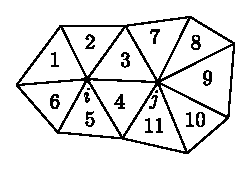
\includegraphics{figures/2023-06-21-dofs-and-supports}
      \caption{Global DoFs $(i, j)$ and their supports}
      \label{fig:dofs-and-supports}
    \end{figure}
  \end{itemize}
\end{itemize}

\begin{mycomment}
  All pointer increment should be taken modulus with respect to the capacity of the ring buffer.
\end{mycomment}

\subsubsection{Ranges formed by ring buffer pointers}

With the above definition of four pointers, the following ranges are naturally derived:
\begin{itemize}
\item Range for quadrature tasks during creation:
  $$
  \begin{cases}
    [\text{tail\_committed}, \text{tail\_pending}) & \text{tail\_pending} \geq
    \text{tail\_committed} \\
    [\text{tail\_committed}, \text{capacity}) \cup [0, \text{tail\_pending}) &
    \text{tail\_pending} < \text{tail\_committed}
  \end{cases}
  $$
  When $\text{tail\_pending} - \text{tail\_committed}$ is zero, there are no active
  producer threads.
\item Range for created quadrature tasks that are ready for processing:
  $$
  \begin{cases}
    [\text{head\_pending}, \text{tail\_committed}) & \text{tail\_committed} \geq
    \text{head\_pending} \\
    [\text{head\_pending}, \text{capacity}) \cup [0, \text{tail\_committed}) &
    \text{tail\_committed} < \text{head\_pending}
  \end{cases}
  $$
\item Range for quadrature tasks during processing:
  $$
  \begin{cases}
    [\text{head\_committed}, \text{head\_pending}) & \text{head\_pending} \geq
    \text{head\_committed} \\
    [\text{head\_committed}, \text{capacity}) \cup [0, \text{head\_pending}) &
    \text{head\_pending} < \text{head\_committed}
  \end{cases}
  $$
  When $\text{head\_pending} - \text{head\_committed}$ is zero, there are no active
  consumer threads.
\item Range for all types of quadrature tasks in the ring buffer, which is a union of the
  above ranges:
  $$
  \begin{cases}
    [\text{head\_committed}, \text{tail\_pending}) & \text{tail\_pending} \geq
    \text{head\_committed} \\
    [\text{head\_committed}, \text{capacity}) \cup [0, \text{tail\_pending}) &
    \text{tail\_pending} < \text{head\_committed}
  \end{cases}
  $$
  \begin{itemize}
  \item When the ring buffer is empty: $\text{tail\_pending} = \text{head\_committed}$
  \item When the ring buffer is full:
    $(\text{tail\_pending} + 1) \% \text{capacity} = \text{head\_committed}$
  \end{itemize}
\end{itemize}

\begin{mycomment}
  The modulo operation used in ring buffer pointer increment is replaced by conditional
  expression for performance issue:
  $$
  (\text{tail\_pending} + \text{incr\_steps}) \geq \text{capacity} ?
  (\text{tail\_pending} + \text{incr\_steps} - \text{capacity}) :
  (\text{tail\_pending} + \text{incr\_steps})
  $$
\end{mycomment}

\subsubsection{Typical ring buffer states}

In the following illustrations, I use $Pn$ to represent a quadrature task which is to be
created by producer $n$ and $Cn$ to represent a task which has been fetched and to be
processed by consumer $n$. I use the red color to indicate the task has been requested for
creation or processing and use the green color to indicate the task has been created or
processed.

\begin{itemize}
\item Initial empty ring buffer
  \begin{center}
    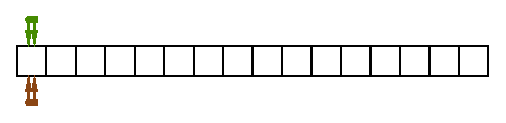
\includegraphics[width=0.6\textwidth,
    keepaspectratio]{figures/2023-05-10-ring-buffer-initial-empty}
    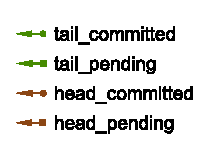
\includegraphics{figures/2023-05-10-ring-buffer-pointer-symbols}
  \end{center}
\item Assume there are three producers which have requested to insert three tasks
  $P1, P2, P3$. Because the three producers run parallel in different threads $1 \sim 3$,
  the thread indices of the requested three tasks are not in the ascending order. At this
  stage, the three tasks are still being prepared, so the pointer \texttt{tail\_committed}
  has not moved forward and the number of tasks ready for processing is still zero.
  \begin{center}
    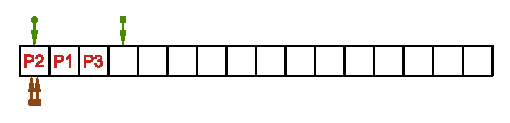
\includegraphics[width=0.6\textwidth,
    keepaspectratio]{figures/2023-05-10-ring-buffer-add-three-tasks}
    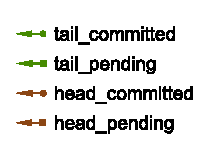
\includegraphics{figures/2023-05-10-ring-buffer-pointer-symbols}
  \end{center}
\item When the task $P1$ is created, the pointer \texttt{tail\_committed} does not move,
  because the creation of $P2$ is not finished. This mechanism ensures that all tasks in
  the range $[\texttt{head\_pending}, \text{tail\_committed})$ are ready for processing.
  \begin{center}
    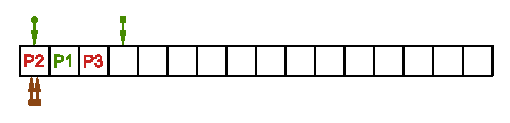
\includegraphics[width=0.6\textwidth,
    keepaspectratio]{figures/2023-05-10-ring-buffer-add-three-tasks-one-finished}
    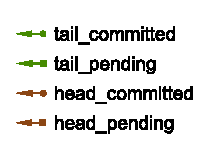
\includegraphics{figures/2023-05-10-ring-buffer-pointer-symbols}
  \end{center}
\item When $P2$ is ready, which was previously pointed by \texttt{tail\_committed},
  \texttt{tail\_committed} moves forward to $P1$. Since $P1$ has also been created,
  \texttt{tail\_committed} continues to move a step further and stops at $P3$.
  \begin{center}
    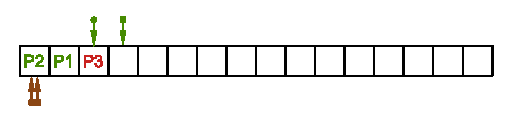
\includegraphics[width=0.6\textwidth,
    keepaspectratio]{figures/2023-05-10-ring-buffer-add-three-tasks-two-finished}
    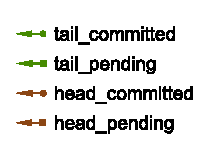
\includegraphics{figures/2023-05-10-ring-buffer-pointer-symbols}
  \end{center}
\item When $P3$ is ready, the pointer \texttt{tail\_committed} moves forward and overlap
  with \texttt{tail\_pending}. Up to now, all tasks requested to be added have been
  created.
  \begin{center}
    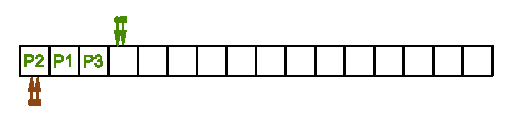
\includegraphics[width=0.6\textwidth,
    keepaspectratio]{figures/2023-05-10-ring-buffer-add-three-tasks-all-finished}
    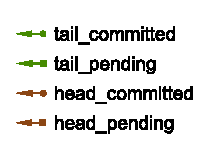
\includegraphics{figures/2023-05-10-ring-buffer-pointer-symbols}
  \end{center}
\item Assume there are two consumers in different threads. Each of them has fetched a task
  for further processing. Then the pointer \texttt{head\_pending} moves forward to $P3$.
  \begin{center}
    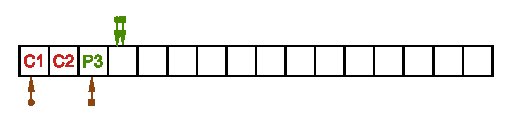
\includegraphics[width=0.6\textwidth,
    keepaspectratio]{figures/2023-05-10-ring-buffer-fetch-two-tasks}
    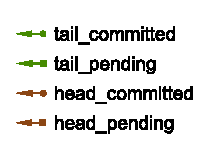
\includegraphics{figures/2023-05-10-ring-buffer-pointer-symbols}
  \end{center}
\item It’s possible that the processing of $C2$ is finished before $C1$. In this case,
  the pointer \texttt{head\_committed} does not move and still points to $C1$.
  \begin{center}
    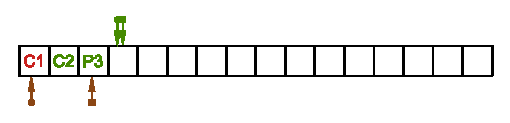
\includegraphics[width=0.6\textwidth,
    keepaspectratio]{figures/2023-05-10-ring-buffer-fetch-two-tasks-one-finished}
    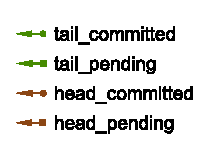
\includegraphics{figures/2023-05-10-ring-buffer-pointer-symbols}
  \end{center}
\item When $C1$ is processed, \texttt{head\_committed} moves forward to $ C2$. Since $C2$
  has also been processed, \texttt{head\_committed} moves a step further and overlaps with
  \texttt{head\_pending}. Now, there are no task during processing
  \begin{center}
    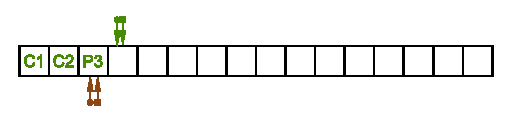
\includegraphics[width=0.6\textwidth,
    keepaspectratio]{figures/2023-05-10-ring-buffer-fetch-two-tasks-all-finished}
    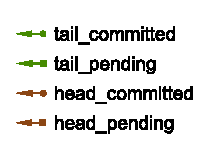
\includegraphics{figures/2023-05-10-ring-buffer-pointer-symbols}
  \end{center}
\item Then the task $P3$ is fetched and processed by consumer $1$. Now all pointers perch
  at a same location and the ring buffer is empty.
  \begin{center}
    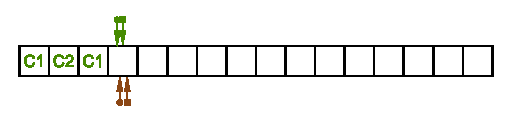
\includegraphics[width=0.6\textwidth,
    keepaspectratio]{figures/2023-05-10-ring-buffer-all-tasks-fetched-and-processed}
    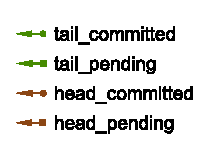
\includegraphics{figures/2023-05-10-ring-buffer-pointer-symbols}
  \end{center}
\item This is the condition when the ring buffer is full:
  $(\text{tail\_pending} + 1) \% \text{capacity} = \text{head\_committed}$.
  \begin{center}
    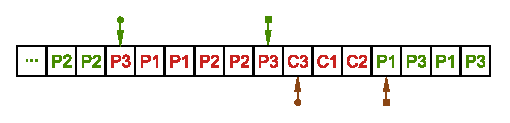
\includegraphics[width=0.6\textwidth,
    keepaspectratio]{figures/2023-05-10-ring-buffer-full}
    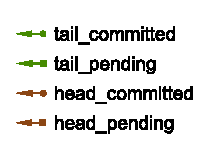
\includegraphics{figures/2023-05-10-ring-buffer-pointer-symbols}
  \end{center}
\end{itemize}

\section{Sauter quadrature for building far field $\mathcal{H}$-matrices}

\chapter{$\mathcal{H}$-matrix}

\section{$\mathcal{H}$-matrix features}

Several member variables are defined for the class \texttt{HMatrix} which describes the
matrix features.

\begin{enumerate}
\item \texttt{State}: this property indicates what is actually stored in the
  \texttt{HMatrix}. After various matrix operations having been applied to the matrix, its
  contents may be changed. For example,
  \begin{itemize}
  \item after calling the in situ version of \texttt{compute\_lu\_factorization}, the
    matrix stores the resulted $L$ and $U$\footnote{$L$ is a normed lower triangular
      matrix, whose diagonal entries are 1. $U$ is an upper triangular matrix. Therefore,
      for the storage of $L$ and $U$ into a single matrix, $U$ is stored as intact, while
      $L$ is stored without its diagonal entries.}, which should have the state
    \texttt{lu};
  \item after calling the in situ version of \texttt{compute\_cholesky\_factorization},
    the matrix stores only the lower triangular $L$ matrix. Being different from $L$
    returned by the LU factorization, $L$ here is usually not normed.
  \end{itemize}
\item \texttt{BlockType}: it is \emph{not} whether the $\mathcal{H}$-matrix node \emph{itself} is
  an upper or lower triangular matrix, but stands for the location of the
  $\mathcal{H}$-matrix node within the top level $\mathcal{H}$-matrix (see Figure
  \ref{fig:hmat-node-block-types}).
  \begin{figure}[htbp]
    \centering
    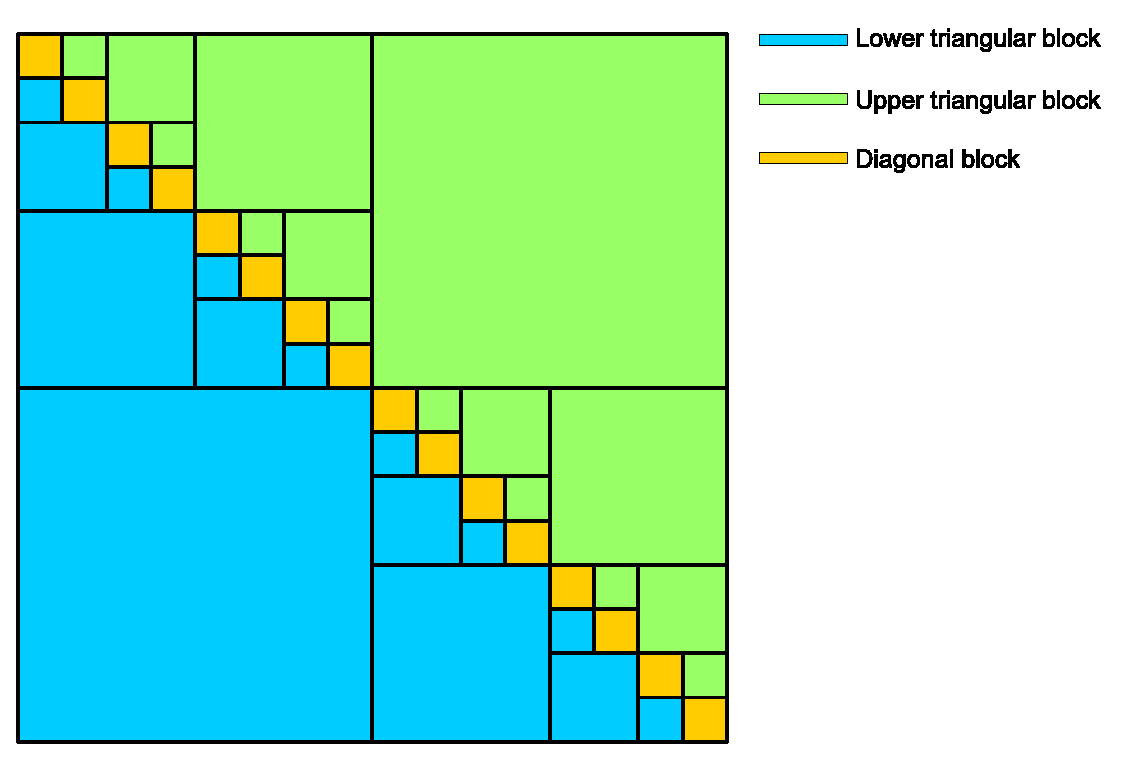
\includegraphics[width=0.5\textwidth, height=\textheight, keepaspectratio]{figures/2023-01-23-hmat-block-type.eps}
    \caption{Block types of a $\mathcal{H}$-matrix node.}
    \label{fig:hmat-node-block-types}
  \end{figure}
\item \texttt{Property}: it specifies whether the $\mathcal{H}$-matrix is symmetric, lower
  triangular or upper triangular. For these cases, only a part of the matrix entries are
  stored and implementing matrix operations, such as matrix addition, matrix-vector
  multiplication, special treatment should be made.
  \begin{itemize}
  \item \texttt{general}: all the $\mathcal{H}$-matrix nodes in the $\mathcal{H}$-matrix
    hierarchy are created and allocated with memory.
  \item \texttt{symmetric}: only the diagonal blocks (which must belong to the near field)
    and matrix blocks in the lower triangular part\footnote{A matrix block is in the lower
      (upper) triangular part is equivalent to say it has the lower (upper) triangular
      block type.} are created and allocated with memory.

    For diagonal matrix blocks, memory is still allocated for the associated whole full
    matrix, but only the lower triangular matrix entries (including diagonal) are filled
    during matrix assembly and included into algebraic matrix computation.

    For matrix blocks in the upper triangular part, basic matrix information, such as
    dimension, associated block cluster node, etc., is still initialized and maintained,
    but the memory is not allocated. When performing matrix operations such as
    matrix-vector multiplication, the contribution from these blocks in the upper
    triangular part should be taken into account by transposing their counterparts in the
    lower triangular part.
  \item \texttt{upper\_triangular}: only the matrix blocks in the upper triangular part and
    the diagonal blocks are created and allocated with memory. The matrix blocks in the
    lower triangular part have only basic matrix information but no memory is allocated.
  \item \texttt{lower\_triangular}: only the matrix blocks in the lower triangular part and
    the diagonal blocks are created and allocated with memory. The matrix blocks in the
    upper triangular part have only basic matrix information but no memory is allocated.
  \end{itemize}
\end{enumerate}

\subsection{Recursively assign $\mathcal{H}$-matrix node block types}
\begin{enumerate}
\item The block type of the top level $\mathcal{H}$-matrix node is diagonal block;
\item Assume the block cluster tree is a quad-tree. If the cluster $\sigma$ and $\tau$
  are divided as $[\sigma_1, \sigma_2]$ and $[\tau_1, \tau_2]$, the array of children of
  the parent block cluster $\sigma\times\tau$ is organized as
  $[(\sigma_1, \tau_1), (\sigma_1, \tau_2), (\sigma_2, \tau_1), (\sigma_2, \tau_2)]$,
  i.e.
  $$
  \begin{pmatrix}
    (\sigma_1, \tau_1) & (\sigma_1, \tau_2) \\
    (\sigma_2, \tau_1) & (\sigma_2, \tau_2)
  \end{pmatrix}
  $$

  If the current $\mathcal{H}$-matrix node has the diagonal block type, then
  $\sigma_1 \equiv \tau_1$ and $\sigma_2 \equiv \tau_2$. If it is not a leaf node, then
  its first child submatrix $(\sigma_1, \tau_1) = (\sigma_1, \sigma_1)$ and last child
  submatrix $(\sigma_2, \sigma_2)$ are still diagonal blocks. The second child submatrix
  $(\sigma_1, \tau_2) = (\sigma_1, \sigma_2)$ has the upper triangular block type and
  the third child submatrix $(\sigma_2,\tau_1) = (\sigma_2,\sigma_1)$ has the lower
  triangular block type.
\item If the current $\mathcal{H}$-matrix node, which is not a leaf node, has the upper
  (lower) triangular block type, all of its children have the upper (lower) triangular
  block type.
\end{enumerate}  

\subsection{Recursively assign $\mathcal{H}$-matrix node properties}

\begin{enumerate}
\item When the property of the top level $\mathcal{H}$-matrix node is \texttt{general}, all descendant
  $\mathcal{H}$-matrix nodes have the \texttt{general} property.
\item When the property of the top level $\mathcal{H}$-matrix node is \texttt{symmetric}:
  \begin{enumerate}
  \item All diagonal blocks on all levels in the $\mathcal{H}$-matrix hierarchy have the
    same \texttt{symmetric} property.
  \item All lower triangular blocks on all levels in the $\mathcal{H}$-matrix hierarchy
    have the \texttt{general} property.
  \item All upper triangular blocks on all levels in the $\mathcal{H}$-matrix hierarchy
    have the \texttt{general} property.
  \end{enumerate}  
\end{enumerate}

\section{General workflow for $\mathcal{H}$-matrix construction}

An \(\mathcal{H}\)-matrix are associated with two DoF handlers, which correspond
respectively to the test space and trial space for discretizing the related bilinear form.
In my current implementation, there are four cases about these DoF handlers:
\begin{enumerate}
\item a same finite element on a same triangulation, e.g. the matrix $\mathscr{V}$ for the
  single layer potential boundary operator in a pure Dirichlet Laplace problem;
\item a same finite element on two different triangulations, e.g. the matrix $\mathscr{V}$
  for the single layer potential boundary operator on the right hand side of the equation
  in a mixed boundary value Laplace problem;
\item two different finite elements on a same triangulation, e.g. the matrix $\mathscr{K}$
  for the double layer potential boundary operator in a pure Dirichlet Laplace problem;
\item two different finite elements on two different triangulations, e.g. the matrix
  $\mathscr{K}$ for the double layer potential boundary operator on the left hand side of
  the equation in a mixed boundary value Laplace problem;
\end{enumerate}

The general workflow for $\mathcal{H}$-matrix construction is as follows.
\begin{itemize}
\item Generate the list(s) of DoF indices (starting from zero in my convention) for the DoF
  handler(s) associated with the $\mathcal{H}$-matrix.
\item Extract the list(s) of coordinates for the DoF support points held within the DoF handler(s).
\item Estimate the average mesh cell sizes at support points.
\item Create cluster tree(s) for DoF handlers.
  \begin{itemize}
  \item Call a constructor to initialize.
  \item Perform the support point based partition.
  \end{itemize}
\item Create block cluster tree(s) from the cluster tree(s).
  \begin{itemize}
  \item Call a constructor to initialize.
  \item Perform the support point based partition.
  \end{itemize}
\item Initialize the \(\mathcal{H}\)-matrix from the block cluster tree.
\item Calculate entries in the $\mathcal{H}$-matrix using ACA (see Section \ref{sec:aca}).
\end{itemize}

\section{$\mathcal{H}$-matrix construction parameter tuning and selection}

\begin{itemize}
\item According to \cite{KriemannParallel2005a}, the typical value of $n_{\min}$ is about
  30-60 in most practical applications.
\end{itemize}

\section{$\mathcal{H}$-matrix fundamental algebraic operation}

\subsection{Matrix-Vector multiplication}
\label{sec:hmat-vmult}

\subsubsection{Matrix-Vector multiplication in $\mathcal{H}$-matrix algebra should be accumulative}

Matrix-vector multiplication is intrinsically accumulative, i.e. the result vector is obtained by
collecting the product vector for each block cluster $b=\tau\times\sigma$ in the partition $P$. Such
accumulation is similar to the assembly of FEM matrix.

In the classical version of matrix-vector multiplication for full matrices, such as that provided
for LAPACK matrices, there are usually two versions: one performs the calculation $y \coloneqq Mx$,
which directly overwrites the result vector $y$; the other is additive, $y \coloneqq y + Mx$. For
matrix-vector multiplication in $\mathcal{H}$-matrix algebra, there is only the additive version,
since the operation is intrinsically accumulative.

According to Equation (7.1) in \cite{HackbuschHierarchical2015}, $MVM(y, M, x, b)$
recursively calls $MVM(y, M, x, b')$, where $b'\in S(b)$. If $MVM$ is implemented as the
``overwriting'' version, $MVM(y, M, x, b')$ will clear the values in $y$ as well as any other
recursive calls of $MVM$. This violates the accumulative behavior required by the matrix-vector
multiplication in $\mathcal{H}$-matrix algebra.

\subsection{Matrix-Matrix multiplication}

Basic considerations about Algorithm \ref{algo:mmr}:
\begin{itemize}
\item $\widetilde{M}_0 = M\big\vert_{\tau_0\times\rho_0}$,
  $\widetilde{M} = M\big\vert_{\tau\times\rho}$,
  $\widetilde{M}_1 = M_1\big\vert_{\tau\times\sigma}$,
  $\widetilde{M}_2 = M_2\big\vert_{\sigma\times\rho}$
\item This function \texttt{MMR} is recursive, hence $\tau_0\times\rho_0$ is the block cluster
  $\tau\times\rho$ when it is called for the first time.
\item $\widetilde{M}$ on $\tau\times\rho$ should belong to the leaf set of the product matrix
  in the first call of this function, i.e. $\tau_0\times\rho_0 \in P$. In further recursive
  call, we can only ensure there exists a $b \in P$ such that $\tau\times\rho \subset b \in P$
  and this $b$ is just $\tau_0\times\rho_0$. This is caused by the fact that even though the
  original block cluster $\tau\times\rho$ in the product matrix belongs to the leaf set of
  $T(I\times K, P)$, the block clusters associated with the two operands $\widetilde{M}_1$ and
  $\widetilde{M}_2$ have children, which produce smaller block matrix in the result. This also
  explains why the block cluster tree $T_{\rm ind}$ introduced in the general
  $\mathcal{H}$-matrix multiplication is usually finer than $T'$ and $T''$.
\item Based on the above consideration, the initial product matrix $\widetilde{M}_0$ is passed
  as an argument, from which the block cluster $b$ can be obtained. Whether $b \in P^+$ or
  $b \in P^-$ determines the format of the corresponding result matrix block.
\item Clusters $\tau$, $\sigma$, $\rho$ are already associated with the input matrices, so
  they do not appear in the argument list.
\item $\widetilde{M}_1 \cdot \widetilde{M}_2$ is just one of the terms contributing to the
  result matrix $\widetilde{M}$, since
  $$
  \widetilde{M} = \sum_{\sigma\in\Sigma}\widetilde{M}_1 \cdot \widetilde{M}_2 =
  \sum_{\sigma\in\Sigma} M_1\big\vert_{\tau\times\sigma} \cdot
  M_2\big\vert_{\sigma\times\rho},
  $$
  where $\Sigma$ is a partition of the index set $J$. Hence its evaluation should be appended
  to $\widetilde{M}$.
\end{itemize}

\begin{breakablealgorithm}
  \label{algo:mmr}
  \caption{Multiplication by starting from a leaf node}
  \begin{algorithmic}[1]\raggedright
  \Procedure{MMR}{$\widetilde{M}_0, \widetilde{M}, \widetilde{M}_1, \widetilde{M}_2$}
    \footnote{Create a local $\mathcal{H}$-matrix $Z$ whose matrix type depends on the initial block
cluster $b = \tau_0\times\rho_0$}
    \If {$\tau_0\times\rho_0 \in P^+$}
      \State {Let $Z$ have \texttt{RkMatrixType} and be associated with the block cluster
$\tau\times\rho$} \footnote{N.B. The block cluster $\tau\times\rho$ is created locally, but not on the heap.}
    \Else \footnote{Case: $\tau_0\times\rho_0 \in P^-$}
      \State {Let $Z$ have FullMatrixType and be associated with the block cluster $\tau\times\rho$}
\footnote{N.B. The block cluster $\tau\times\rho$ is created locally, but no on the heap.}
    \EndIf
    
    \If {$\tau\times\sigma \in P'$ or $\sigma\times\rho \in P''$} \Comment {When either
$\widetilde{M}_1$ or $\widetilde{M}_2$ is a leaf node in its respective $\mathcal{H}$-matrix
hierarchy, we can directly perform the matrix multiplication, whose operands involve either rank-k matrix or full matrix.}

    % \redcomment{In the following, we directly represent $Z$ as a rank-k or % full matrix instead of an $\mathcal{H}$-matrix for this consideration: $Z$ % will be further appended to the result matrix via embedding and formatted % addition; since we do not bother to associate a block cluster node with % $Z$, we will perform the calculation directly instead of using % $\mathcal{H}$-matrix member functions.}

      \State {Initialize local matrices $Z_R$ and $Z_F$ for storing the multiplication results, which will be associated with the local matrix $Z$ and further assembled into the matrix $\widetilde{M}$.}
    
      \If {$\widetilde{M}_1 \in \mathcal{R}$}
        \State {Apply $\mathcal{R}\times\mathcal{H} \rightarrow \mathcal{R}$ for $Z_R :=
\widetilde{M}_1 \cdot \widetilde{M}_2$}
      \ElsIf {$\widetilde{M}_2 \in \mathcal{R}$}
        \State {Apply $\mathcal{H}\times\mathcal{R} \rightarrow \mathcal{R}$ for $Z_R :=
\widetilde{M}_1 \cdot \widetilde{M}_2$}
      \ElsIf {$\widetilde{M}_1 \in \mathcal{F}$}
        \State {Apply $\mathcal{F}\times\mathcal{H} \rightarrow \mathcal{F}$ for $Z_F :=
\widetilde{M}_1 \cdot \widetilde{M}_2$}
      \ElsIf {$\widetilde{M}_2 \in \mathcal{F}$}
        \State {Apply $\mathcal{H}\times\mathcal{F} \rightarrow \mathcal{F}$ for $Z_F :=
\widetilde{M}_1 \cdot \widetilde{M}_2$}
      \EndIf

      \If {$\tau_0\times\rho_0 \in P^+$} \Comment{If the top level result of the matrix product, when
this function is called for the first time, is a rank-k matrix}
        \If {the result of the matrix product for the current level is a full matrix, i.e. $Z_F$}
          \State $Z_R := \mathcal{T}_r^{\mathcal{R}}(Z_F)$ \Comment{Truncate the full matrix to an
rank-k matrix}
        \EndIf
        \State Associate $Z_R$ with $Z$
      \Else \Comment {Case: $\tau_0\times\rho_0 \in P^-$, i.e. the top level result of the matrix
product is a full matrix}
        \If {the result of the matrix product for the current level is a rank-k matrix, i.e. $Z_R$}
          \State $Z_F := \mathcal{T}^{\mathcal{F} \leftarrow \mathcal{R}}(Z_R)$ \Comment{Convert the
rank-k matrix to a full matrix}
        \EndIf
        \State Associate $Z_F$ with $Z$
      \EndIf
    \Else \Comment {Case: $\tau\times\sigma \notin P'$ and $\sigma\times\rho \notin P''$, which
means both the two operands $\widetilde{M}_1$ and $\widetilde{M}_2$ have children, hence multiplication of submatrices should be performed.}
    
      \Comment{Next, perform multiplication of submatrices in $\widetilde{M}_1$ and $\widetilde{M}_2$:
        $$
        \begin{aligned} \widetilde{M}_1\cdot\widetilde{M}_2 &=
          \begin{pmatrix} \widetilde{M}_1[0] & \widetilde{M}_1[1] \\ \widetilde{M}_1[2] &
            \widetilde{M}_1[3]
        \end{pmatrix} \cdot
        \begin{pmatrix} \widetilde{M}_2[0] & \widetilde{M}_2[1] \\ \widetilde{M}_2[2] &
          \widetilde{M}_2[3]
        \end{pmatrix} \\ &=
        \begin{pmatrix} \widetilde{M}_1[0]\widetilde{M}_2[0] + \widetilde{M}_1[1]\widetilde{M}_2[2] &
          \widetilde{M}_1[0]\widetilde{M}_2[1] + \widetilde{M}_1[1]\widetilde{M}_2[3] \\
          \widetilde{M}_1[2]\widetilde{M}_2[0] + \widetilde{M}_1[3]\widetilde{M}_2[2] &
          \widetilde{M}_1[2]\widetilde{M}_2[1] + \widetilde{M}_1[3]\widetilde{M}_2[3]
        \end{pmatrix}
        \end{aligned}
        $$
        From this we can see that there are eight multiplication operations for submatrices.}

      \State {MMR($\widetilde{M}_0, Z, \widetilde{M}_1[0], \widetilde{M}_2[0]$)}
      \State {MMR($\widetilde{M}_0, Z, \widetilde{M}_1[1], \widetilde{M}_2[2]$)}
      \State {MMR($\widetilde{M}_0, Z, \widetilde{M}_1[0], \widetilde{M}_2[1]$)}
      \State {MMR($\widetilde{M}_0, Z, \widetilde{M}_1[1], \widetilde{M}_2[3]$)}
      \State {MMR($\widetilde{M}_0, Z, \widetilde{M}_1[2], \widetilde{M}_2[0]$)}
      \State {MMR($\widetilde{M}_0, Z, \widetilde{M}_1[3], \widetilde{M}_2[2]$)}
      \State {MMR($\widetilde{M}_0, Z, \widetilde{M}_1[2], \widetilde{M}_2[1]$)}
      \State {MMR($\widetilde{M}_0, Z, \widetilde{M}_1[3], \widetilde{M}_2[3]$)}
    \EndIf
    
    \Comment{Finally, assemble the local result matrix $Z$ into the matrix $\widetilde{M}$}
    \If {$\tau_0\times\rho_0 \in P^+$} \Comment {$Z$ has \texttt{RkMatrixType}}
      \State {Embed the rank-k matrix to have the same size as the larger matrix, then perform
formatted addition.}
    \Else \Comment {$Z$ has \texttt{FullMatrixType}}
      \State {Directly assemble the full matrix to the larger matrix.}
    \EndIf
  \EndProcedure
  \end{algorithmic}
\end{breakablealgorithm}

\begin{breakablealgorithm}
  \caption{Multiplication of level-conserving $\mathcal{H}$-matrices}
  \label{algo:hmat-mmult-level-conserving}
  \begin{algorithmic}[1]
  \Procedure{MM}{$M, M_1, M_2$}
    \If {$\tau\times\sigma \notin P'$ and $\sigma\times\rho \notin P''$ and $\tau\times\rho \notin
P$} \Comment {When all matrices (two operands and one product) are not leaf nodes, perform multiplication of submatrices:
      $$
      \begin{pmatrix} M[0] & M[1] \\ M[2] & M[3]
      \end{pmatrix} =
      \begin{pmatrix} M_1[0]M_2[0] + M_1[1]M_2[2] & M_1[0]M_2[1] + M_1[1]M_2[3] \\ M_1[2]M_2[0] + M_1[3]M_2[2] & M_1[2]M_2[1] + M_1[3]M_2[3]
      \end{pmatrix}
      $$}
      \State {MM($M[0], M_1[0], M_2[0]$)}
      \State {MM($M[0], M_1[1], M_2[2]$)}
      \State {MM($M[1], M_1[0], M_2[1]$)}
      \State {MM($M[1], M_1[1], M_2[3]$)}
      \State {MM($M[2], M_1[2], M_2[0]$)}
      \State {MM($M[2], M_1[3], M_2[2]$)}
      \State {MM($M[3], M_1[2], M_2[1]$)}
      \State {MM($M[3], M_1[3], M_2[3]$)}
    \ElsIf {$\tau\times\rho \notin P$} \Comment{Case: one of the operands is a leaf node while the
result matrix block can still be split.}
      \State {Create a rank-k matrix $Z$ on the block cluster $\tau\times\rho$}

      \If {$M_1 \in \mathcal{R}$}
        \State {Apply $\mathcal{R}\times\mathcal{H} \rightarrow \mathcal{R}$ for $Z := M_1M_2$}
      \ElsIf {$M_2 \in \mathcal{R}$}
        \State {Apply $\mathcal{H}\times\mathcal{R} \rightarrow \mathcal{R}$ for $Z := M_1M_2$}
      \ElsIf {$M_1 \in \mathcal{F}$}
        \State {Apply $\mathcal{F}\times\mathcal{H} \rightarrow \mathcal{R}$ for $Z := M_1M_2$}
      \ElsIf {$M_2 \in \mathcal{F}$}
        \State {Apply $\mathcal{H}\times\mathcal{F} \rightarrow \mathcal{R}$ for $Z := M_1M_2$}
      \EndIf

      \State {Add $Z$ into $M$ via $\mathcal{R} \oplus_r \mathcal{H} \rightarrow \mathcal{H}$.} \Comment {Since $M$ has descendants, the rank-k matrix $Z$ needs to be restricted to each leaf node of $M$ and then perform addition with full leaf matrix or formatted addition with rank-k leaf matrix.}
      
    \Else \Comment {Case: $\tau\times\rho \in P$, while there is no ``leaf node'' requirement on the operands.}
      \State {\hyperref[algo:mmr]{MMR}($M, M, M_1, M_2$)}
    \EndIf
  \EndProcedure
  \end{algorithmic}
\end{breakablealgorithm}

\section{$\mathcal{H}$-matrix solvers}

\subsection{Forward substitution: $Lx=b$}
\label{sec:forward-subst}

Let's start from the forward substitution for a full matrix. Let $L\in \mathbb{R}^{n\times
  n}$ be a lower triangular matrix, $x, b\in \mathbb{R}^n$. Solve the problem $Lx=b$,
\begin{equation}
\begin{pmatrix}
  a_{11} & & & & \\
  a_{21} & a_{22} & & &\\
  a_{31} & a_{32} & a_{33} & & \\
  \vdots & \vdots & \vdots & \ddots & \\
  a_{n1} & \cdots & \cdots & \cdots & a_{nn}
\end{pmatrix}
\begin{pmatrix}
  x_1 \\ x_2 \\ x_3 \\ \vdots \\ x_n
\end{pmatrix} =
\begin{pmatrix}
  b_1 \\ b_2 \\ b_3 \\ \vdots \\ b_n
\end{pmatrix}.
\end{equation}
From the first row, we have $x_1 = \frac{b_1}{a_{11}}$, assuming $a_{11}\neq 0$. Then from
the second row, we have $x_2 = \frac{b_2 - a_{21}x_1}{a_{22}}$. For the $i$-th row,
\begin{equation}
  x_i = \frac{b_i - \sum_{j=1}^{i-1} a_{ij}x_j}{a_{ii}}.
\end{equation}
Each $x_i$ depends on $b_i$ and on all previous $x_j$ with $j=1, \cdots, i-1$. Hence,
$x_i$ depends on all $b_j$ with $j=1, \cdots, i$. Therefore, the forward substitution can
be performed in situ, i.e. the right hand side vector $b$ can be overwritten by the
solution vector $x$ and there is no need to allocate additional memory for $x$. The
algorithm of forward substitution for a full matrix is show in \ref{algo:forward-subst-full}.
\begin{breakablealgorithm}
  \label{algo:forward-subst-full}
  \caption{Forward substitution for a lower triangular full matrix}
  \begin{algorithmic}[1]
    \Procedure{ForwardSubstF}{$L, b$}
      \For {each row of $L$: $i=1, \cdots, n$}
        \For {each column before the $i$-th column: $j=1, \cdots, i-1$}
          \State {$b_i \coloneqq b_i - a_{ij} x_j$}
        \EndFor
        \State {$x_i\coloneqq \frac{b_i}{a_{ii}}$}
      \EndFor
    \EndProcedure
  \end{algorithmic}
\end{breakablealgorithm}

A variant of the problem $Lx=b$ is $xU = b$, which is equivalent to $U^{\mathrm{T}}x = b$.
This can still be solved by the work flow of forward substitution, which is summarized in Algorithm \ref{algo:forward-subst-full-transposed}.
\begin{breakablealgorithm}
  \label{algo:forward-subst-full-transposed}
  \caption{Forward substitution for an upper triangular full matrix}
  \begin{algorithmic}[1]
    \Procedure{ForwardSubstFT}{$U, b$}
      \For {each column of $U$: $j=1, \cdots, n$}
        \For {each row before the $j$-th row: $i=1, \cdots, j-1$}
          \State {$b_j \coloneqq b_j - a_{ji} x_i$}
        \EndFor
        \State {$x_j \coloneqq \frac{b_j}{a_{jj}}$}
      \EndFor
    \EndProcedure
  \end{algorithmic}
\end{breakablealgorithm}

Algorithm \ref{algo:forward-subst-full} and \ref{algo:forward-subst-full-transposed}
correspond to a same LAPACK function \texttt{trsv}.

When the matrix is an $\mathcal{H}$-matrix, let it be written as
$L\big\vert_{\tau\times \tau}$. Assume the cluster $\tau$ has $p$ children. Then this
$\mathcal{H}$-matrix has the following block structure:
\begin{equation}
  \begin{pmatrix}
    L_{11} & & & \\
    L_{21} & L_{22} & & \\
    \vdots & \vdots & \ddots & \\
    L_{p1} & L_{p2} & \cdots & L_{pp}
  \end{pmatrix}.
\end{equation}
Each block in the above matrix is actually
$L_{ij} \coloneqq L\big\vert_{\tau[i]\times\tau[j]}$, with $\tau[i]$ being the $i$-th
child of the cluster $\tau$. Also note that the diagonal blocks
$L\big\vert_{\tau[i]\times\tau[i]}$ are lower triangular matrices not general matrices on
the diagonal line.

To solve $L\big\vert_{\tau\times\tau}x\big\vert_{\tau}=b\big\vert_{\tau}$ we still apply
the work flow of the forward substitution for a full matrix, but replace the scalar value
computation in $x_i$ with $\mathcal{H}$-matrix operations. In this way, the forward
substitution for an $\mathcal{H}$-matrix naturally becomes recursive. The algorithm is
shown in Algorithm \ref{algo:forward-subst-hmat}.
\begin{breakablealgorithm}
  \label{algo:forward-subst-hmat}
  \caption{Forward substitution for a lower triangular $\mathcal{H}$-matrix}
  \begin{algorithmic}[1]
    \Procedure{ForwardSubstH}{$L\big\vert_{\tau\times\tau}, b \big\vert_{\tau}$}
      \If {$L\big\vert_{\tau\times\tau} \in P$} \Comment{Because
$L\big\vert_{\tau\times\tau}$ is a diagonal block, i.e. the row block cluster is the same
as the column block cluster, it belongs to $P^-$ and is a full matrix.}
        \State{Solve $L\big\vert_{\tau\times\tau} x\big\vert_{\tau} = b\big\vert_{\tau}$
using the forward substitution for a full matrix:\\\textsc{ForwardSubstF}($L\big\vert_{\tau\times\tau}, b \big\vert_{\tau}$)}
      \Else
        \For {each block row of $L\big\vert_{\tau\times\tau}$: $i=1, \cdots, \#S(\tau)$}
          \For {each block column before the $i$-th column: $j=1,\cdots,i-1$}
            \State{$b\big\vert_{\tau[i]} \coloneqq b\big\vert_{\tau[i]} -
L\big\vert_{\tau[i]\times\tau[j]}x\big\vert_{\tau[j]}$}
\Comment{$L\big\vert_{\tau[i]\times\tau[j]}x\big\vert_{\tau[j]}$ is
$\mathcal{H}$-matrix-vector multiplication.}
          \EndFor
          \State{\textsc{ForwardSubstH}($L\big\vert_{\tau[i]\times\tau[i]}, b \big\vert_{\tau[i]}$)}
        \EndFor
      \EndIf
    \EndProcedure
  \end{algorithmic}
\end{breakablealgorithm}

Similar, the variant problem $X \big\vert_{\tau} U \big\vert_{\tau} = b \big\vert_{\tau}$
can be solved by forward substitution in Algorithm
\ref{algo:forward-subst-hmat-transpose}.
\begin{breakablealgorithm}
  \label{algo:forward-subst-hmat-transpose}
  \caption{Forward substitution for an upper triangular $\mathcal{H}$-matrix}
  \begin{algorithmic}[1]
    \Procedure{ForwardSubstHT}{$U\big\vert_{\tau\times\tau}, b \big\vert_{\tau}$}
      \If {$U\big\vert_{\tau\times\tau} \in P$} \Comment{Because
$U\big\vert_{\tau\times\tau}$ is a diagonal block, i.e. the row block cluster is the same
as the column block cluster, it belongs to $P^-$ and is a full matrix.}
        \State{Solve $x\big\vert_{\tau} U\big\vert_{\tau\times\tau} = b\big\vert_{\tau}$
using the forward substitution for a transposed full matrix:\\\textsc{ForwardSubstFT}($U\big\vert_{\tau\times\tau}, b \big\vert_{\tau}$)}
      \Else
        \For {each block column of $U \big\vert_{\tau\times\tau}$: $j=1, \cdots, \#S(\tau)$}
          \For {each block row before the $j$-th row: $i=1,\cdots,j-1$}
            \State{$b\big\vert_{\tau[j]} \coloneqq b\big\vert_{\tau[j]} -
U^{\mathrm{T}}\big\vert_{\tau[j]\times\tau[i]} x\big\vert_{\tau[i]}$}
          \EndFor
          \State{\textsc{ForwardSubstHT}($U\big\vert_{\tau[j]\times\tau[j]}, b \big\vert_{\tau[j]}$)}
        \EndFor
      \EndIf
    \EndProcedure
  \end{algorithmic}
\end{breakablealgorithm}

\subsection{Backward substitution: $Ux=b$}

Let $U\in \mathbb{R}^{n\times n}$ be an upper triangular full matrix. Solve the problem
$Ux=b$
\begin{equation}
  \begin{pmatrix}
    a_{11} & a_{12} & a_{13} & \cdots & a_{1n} \\
    & a_{22} & a_{23} & \cdots & a_{2n} \\
    & & a_{33} & \cdots & a_{3n} \\
    & & & \ddots & \vdots \\
    & & & & a_{nn}
  \end{pmatrix}
  \begin{pmatrix}
    x_1\\x_2\\x_3\\\vdots\\x_n
  \end{pmatrix}=
  \begin{pmatrix}
    b_1\\b_2\\b_3\\\vdots\\b_n
  \end{pmatrix}
\end{equation}
using the backward substitution in Algorithm \ref{algo:backward-subst-full}.
\begin{breakablealgorithm}
  \label{algo:backward-subst-full}
  \caption{Backward substitution for a full matrix}
  \begin{algorithmic}[1]
    \Procedure{BackwardSubstF}{$U, b$}
      \For {each row of $U$: $i=n, n-1, \cdots, 1$}
        \For {each column after the $i$-th column: $j=i+1,\cdots,n$}
          \State{$b_i\coloneqq b_i - a_{ij}x_j$}
        \EndFor
        \State{$x_i\coloneqq \frac{b_i}{a_{ii}}$}
      \EndFor
    \EndProcedure
  \end{algorithmic}
\end{breakablealgorithm}

Algorithm \ref{algo:backward-subst-full} corresponds to the LAPACK function \texttt{trsv}.

Let $U\big\vert_{\tau\times\tau}$ be an upper triangular $\mathcal{H}$-matrix which has
the following block structure:
\begin{equation}
  \begin{pmatrix}
    U_{11} & U_{12} & \cdots & U_{1p} \\
    & U_{22} & \cdots & U_{2p} \\
    & & \ddots & \vdots \\
    & & & U_{pp}
  \end{pmatrix}.
\end{equation}
Solve $U\big\vert_{\tau\times\tau} x \big\vert_{\tau} = b \big\vert_{\tau} $ using
Algorithm \ref{algo:backward-subst-hmat}.
\begin{breakablealgorithm}
  \label{algo:backward-subst-hmat}
  \caption{Backward substitution for an upper triangular $\mathcal{H}$-matrix}
  \begin{algorithmic}[1]
    \Procedure{BackwardSubstH}{$U \big\vert_{\tau\times\tau}, b \big\vert_{\tau}$}
      \If {$U \big\vert_{\tau\times\tau}\in P$}
        \State{Solve $U \big\vert_{\tau\times\tau}x \big\vert_{\tau} = b \big\vert_{\tau}$ using
  the backward substitution for a full matrix:\\\textsc{BackwardSubstF}($U \big\vert_{\tau\times\tau}, b \big\vert_{\tau}$)}
      \Else
        \For {each block row of $U \big\vert_{\tau\times\tau}$: $i=\#S(\tau), \#S(\tau)-1, \cdots,
        1$}
          \For {For each block column after the $i$-th column: $j=i+1,\cdots,\#S(\tau)$}
            \State{$b \big\vert_{\tau[i]} \coloneqq b \big\vert_{\tau[i]} - U
\big\vert_{\tau[i]\times\tau[i]} b \big\vert_{\tau[j]}$}
          \EndFor
        \State{\textsc{BackwardSubstH}($U \big\vert_{\tau[i]\times\tau[i]},b \big\vert_{\tau[i]}$)}
        \EndFor
      \EndIf
    \EndProcedure
  \end{algorithmic}
\end{breakablealgorithm}

\subsection{Matrix-valued forward substitution: $LX = Z$}
\label{sec:forward-subst-matrix-valued}

The problem to be solved is
$L \big\vert_{\tau\times\tau} X \big\vert_{\tau\times\sigma} = Z
\big\vert_{\tau\times\sigma}$, where $L \big\vert_{\tau\times\tau}$ is an
$\mathcal{H}$-matrix constructed with respect to the block cluster tree $T(I\times I, P)$,
$X \big\vert_{\tau\times\sigma}$ and $Z \big\vert_{\tau\times\sigma}$ are
$\mathcal{H}$-matrices constructed with respect to the block cluster tree
$T(I\times J, P')$. If the index set $I$ is different from $J$, or if $I$ is equal to $J$,
but they are partitioned into different cluster trees, the two block cluster trees
$T(I\times I)$ and $T(I\times J)$ may have different leaf sets $P$ and $P'$. Also note the
right hand side term $Z$ and the solution term $X$ are now $\mathcal{H}$-matrices instead
of vectors. That's why the algorithm for solving this problem is called
\emph{matrix-valued} forward substitution. In addition, $X$ and $Z$ are built on a same
block cluster $\tau\times\sigma$, while $L$ is a diagonal block and built on the block
cluster $\tau\times\tau$.

To formulate this algorithm, the following cases should be clarified:
\begin{itemize}
\item When $\tau\times\sigma\in P'^-$, both $X \big\vert_{\tau\times\sigma}$ and
  $Z \big\vert_{\tau\times\sigma}$ are full matrices. Now
  $L \big\vert_{\tau\times\tau} X \big\vert_{\tau\times\sigma} = Z
  \big\vert_{\tau\times\sigma}$ is a multi-right hand side (RHS) problem. For the $j$-th
  column in $X \big\vert_{\tau\times\sigma}$ and $Z \big\vert_{\tau\times\sigma}$, i.e.
  $X \big\vert_{\tau\times\sigma_j}$ and $Z \big\vert_{\tau\times\sigma_j}$ \footnote{Here
    we use $\sigma_j$ to represent the $j$-th index in the index set $\sigma$.}, we can
  solve
  $L \big\vert_{\tau\times\tau} X \big\vert_{\tau\times\sigma_j} = Z
  \big\vert_{\tau\times\sigma_j}$ for $X \big\vert_{\tau\times\sigma_j}$ using
  \textsc{ForwardSubstH}, since $L \big\vert_{\tau\times\tau}$ is still an
  $\mathcal{H}$-matrix.
 \item When $\tau\times\sigma\in P'^+$, both $X \big\vert_{\tau\times\sigma}$ and
  $Z \big\vert_{\tau\times\sigma}$ are rank-$k$ matrices. $Z \big\vert_{\tau\times\sigma}$
  is known and has the low-rank expansion
  $Z \big\vert_{\tau\times\sigma} = A B^{\mathrm{T}}$. $X \big\vert_{\tau\times\sigma}$ is
  unknown and we assume it has the ansatz expansion
  $X \big\vert_{\tau\times\sigma} = A' B^{\mathrm{T}}$, where the second component $B$ is
  adopted as the same in the expansion of $Z \big\vert_{\tau\times\sigma}$. Then the
  equation becomes
  \begin{equation}
    L \big\vert_{\tau\times\tau} A' B^{\mathrm{T}} = A B^{\mathrm{T}}.
  \end{equation}
  $B^{\mathrm{T}}$ on the two sides of the equation can be eliminated and the equation to
  be solved is
  \begin{equation}
    L \big\vert_{\tau\times\tau} A' = A.
  \end{equation}
  Because both $A'$ and $A$ are full matrices, we can use the same method in the previous
  case to solve each column in $A'$.
\item When $\tau\times\sigma\notin P'$, both $X \big\vert_{\tau\times\sigma}$ and $Z
  \big\vert_{\tau\times\sigma}$ have submatrix structures. Because the size of $\tau$ is
  still larger than $n_{\min}$, $L \big\vert_{\tau\times\tau}$ also has a submatrix
  structure. Assume $\#S(\tau) = p$ and $\#S(\sigma) = q$, a matrix-valued equation as below should
  be solved
  \begin{equation}
    \begin{pmatrix}
      L_{11} & & & \\
      L_{21} & L_{22} & & \\
      \vdots & & \ddots & \\
      L_{p1} & L_{p2} & \cdots & L_{pp}
    \end{pmatrix}
    \begin{pmatrix}
      X_{11} & \cdots & X_{1q} \\
      \vdots & \vdots & \vdots \\
      X_{p1} & \cdots & X_{pq}
    \end{pmatrix} =
    \begin{pmatrix}
      Z_{11} & \cdots & Z_{1q} \\
      \vdots & \vdots & \vdots \\
      Z_{p1} & \cdots & Z_{pq}
    \end{pmatrix}.
  \end{equation}
  For the first block row, we have the following $q$ equations
  \begin{equation*}
    L_{11}X_{11} = Z_{11},\; L_{11}X_{12} = Z_{12}, \cdots, L_{11}X_{1q} = Z_{1q}.
  \end{equation*}
  For the second block row, we have
  \begin{equation*}
    L_{21}X_{11} + L_{22}X_{21} = Z_{21}, \cdots, L_{21}X_{1q} + L_{22}X_{2q} = Z_{2q}.
  \end{equation*}
  Then for the $i$-th block row, we have
  \begin{equation*}
    \sum_{k=1}^{i} L_{ik}X_{k1} = Z_{i1}, \cdots, \sum_{k=1}^i L_{ik}X_{kq} = Z_{iq}.
  \end{equation*}
  Equations from the first block row are still matrix-valued lower triangular problems,
  which can be directly solved by one recursive call of this algorithm. So
  $X_{11}, X_{12}, \cdots, X_{1q}$ are obtained.

  For equations from the second block row, we keep the terms related to the diagonal block
  $L_{22}$ on the left hand side and move the other terms to the right hand side,
  \begin{equation*}
    L_{22}X_{21} = Z_{21} - L_{21}X_{11}, \cdots, L_{22}X_{2q} = Z_{2q} - L_{21}X_{1q}.
  \end{equation*}
  With the solutions obtained from the first block row, we can solve
  $X_{21}, \cdots, X_{2q}$ by one recursive call of this algorithm.

  Without loss of generality, for equations from the $i$-th block row, we keep the terms
  related to the diagonal block $L_{ii}$ on the left hand side and move the other terms to
  the right hand side,
  \begin{equation*}
    L_{ii}X_{ij} = Z_{ij} - \sum_{k=1}^{i-1} L_{ik}X_{kj} \quad (j=1,\cdots,q).
  \end{equation*}
  Since $X_{rs}$ with $r=1,\cdots,i-1$ and $s=1,\cdots,q$ have been computed from the
  equations in the first $i-1$ rows, we can solve $X_{i1}, \cdots, X_{iq}$.
\end{itemize}

The above cases can be summarized into Algorithm \ref{algo:forward-subst-matrix-valued}.
\begin{breakablealgorithm}
  \label{algo:forward-subst-matrix-valued}
  \caption{Matrix-valued forward substitution}
  \begin{algorithmic}[1]
    \Procedure{ForwardSubstM}{$L \big\vert_{\tau\times\tau}, X \big\vert_{\tau\times\sigma},
Z \big\vert_{\tau\times\sigma}$}
      \If {$\tau\times\sigma \in P'^-$} \Comment{Both $X
\big\vert_{\tau\times\sigma}$ and $Z \big\vert_{\tau\times\sigma}$ are full matrices.}
        \For {each column of $X \big\vert_{\tau\times\sigma}$ and $Z
\big\vert_{\tau\times\sigma}$: $j=1,\cdots,\#\sigma$}
          \State{Solve $L \big\vert_{\tau\times\tau} X \big\vert_{\tau\times\sigma_j} = Z
  \big\vert_{\tau\times\sigma_j}$ for $X \big\vert_{\tau\times\sigma_j}$ using
  \textsc{ForwardSubstH}.}
        \EndFor
      \ElsIf {$\tau\times\sigma \in P'^+$} \Comment{Both $X
\big\vert_{\tau\times\sigma}$ and $Z \big\vert_{\tau\times\sigma}$ are rank-$k$ matrices.}
        \State {Copy $Z \big\vert_{\tau\times\sigma} = AB^{\mathrm{T}}$ to $X
\big\vert_{\tau\times\sigma}$.}
        \State{Solve $L \big\vert_{\tau\times\tau} A' = A$, where $A'$ is the first
component matrix in $X \big\vert_{\tau\times\sigma}$ via multiple calls of
\textsc{ForwardSubstH}.}
      \Else \Comment{When $\tau\times\sigma \notin P'$, both $X
\big\vert_{\tau\times\sigma}$ and $Z \big\vert_{\tau\times\sigma}$ have submatrix structures.}
        \For {each block row of $Z \big\vert_{\tau\times\sigma}$: $i=1,\cdots,\#S(\tau)$}
          \For {each block column of $Z \big\vert_{\tau\times\sigma}$: $j=1,\cdots,\#S(\sigma)$}
            \For {each block column before the $i$-th column in $L
  \big\vert_{\tau\times\tau}$: $k=1,\cdots,i-1$}
              \State{$Z \big\vert_{\tau[i]\times\sigma[j]} \coloneqq Z
  \big\vert_{\tau[i]\times\sigma[j]} - L \big\vert_{\tau[i]\times\tau[k]}X \big\vert_{\tau[k]\times\sigma[j]}$}
            \EndFor
            \State{\textsc{ForwardSubstM}($L \big\vert_{\tau[i]\times\tau[i]}, X
  \big\vert_{\tau[i]\times\sigma[j]}, Z \big\vert_{\tau[i]\times\sigma[j]}$)}
          \EndFor
        \EndFor
      \EndIf
    \EndProcedure
  \end{algorithmic}
\end{breakablealgorithm}

Now if we carefully observe Algorithm \ref{algo:forward-subst-matrix-valued}, we find out
these points:
\begin{itemize}
\item When the result matrix block $X \big\vert_{\tau\times\sigma}$ belongs to the near
  field set $P'^-$, each of its column vector is independently solved from this equation
  $L \big\vert_{\tau\times\tau} X \big\vert_{\tau\times\sigma_j} = Z
  \big\vert_{\tau\times\sigma_j}$ using \textsc{ForwardSubstH}. Because
  \textsc{ForwardSubstH} can be performed in situ, i.e. the result vector
  $X \big\vert_{\tau\times\sigma_j}$ can be directly obtained by overwriting the right
  hand side vector $Z \big\vert_{\tau\times\sigma_j}$, the solution of the whole matrix
  block $X \big\vert_{\tau\times\sigma}$ can be in situ, i.e. the set of result vectors
  can be directly written into the right hand side matrix block
  $Z \big\vert_{\tau\times\sigma}$.
\item When the result matrix block $X \big\vert_{\tau\times\sigma}$ belongs to the far
  field set $P'^+$, after copying $Z \big\vert_{\tau\times\sigma}$ to
  $X \big\vert_{\tau\times\sigma}$, the solution of $L \big\vert_{\tau\times\tau} A' = A$
  using \textsc{ForwardSubstH} can be in situ. Therefore in this case, the solution of
  $X \big\vert_{\tau\times\sigma}$ can be in situ.
\item When the result matrix block $X \big\vert_{\tau\times\sigma}$ as well as
  $Z \big\vert_{\tau\times\sigma}$ has a submatrix structure, each submatrix block
  $Z \big\vert_{\tau[i]\times\sigma[j]}$ in $Z \big\vert_{\tau\times\sigma}$ is updated
  with the negative product
  $L \big\vert_{\tau[i]\times\tau[k]}X \big\vert_{\tau[k]\times\sigma[j]}$. Because the
  index $k$ is smaller than the current block row index $i$ which has been iterated in
  previous loops, it means the set of equations
  $L \big\vert_{\tau[k]\times\tau[k]} X \big\vert_{\tau[k]\times\sigma[j]} = Z
  \big\vert_{\tau[k]\times\sigma[j]}$ for all $j=1,\cdots,\#S(\sigma)$ have already been
  solved. If these equations are solved in situ, the matrix blocks
  $Z \big\vert_{\tau[k]\times\sigma[j]}$ for all $j=1,\cdots,\#S(\sigma)$ have been
  overwritten with $X \big\vert_{\tau[k]\times\sigma[j]}$ respectively. Then, the update
  of the current right hand side matrix block $Z \big\vert_{\tau[i]\times\sigma[j]}$ can
  be made in situ, i.e.
  $Z \big\vert_{\tau[i]\times\sigma[j]} \coloneqq Z \big\vert_{\tau[i]\times\sigma[j]} - L
  \big\vert_{\tau[i]\times\tau[k]}Z \big\vert_{\tau[k]\times\sigma[j]}$.
\end{itemize}
In this way, Algorithm \ref{algo:forward-subst-matrix-valued} can be performed in situ.

\subsection{Matrix-valued forward substitution for an upper triangular $\mathcal{H}$-matrix: $XU = Z$}

The equation to be solved is
$X \big\vert_{\tau\times\sigma} U \big\vert_{\sigma\times\sigma} = Z
\big\vert_{\tau\times\sigma}$, where $U \big\vert_{\sigma\times\sigma}$ is an
$\mathcal{H}$-matrix constructed with respect to the block cluster tree $T(J\times J, P)$,
while $X \big\vert_{\tau\times\sigma}$ and $Z \big\vert_{\tau\times\sigma}$ are
$\mathcal{H}$-matrices constructed with respect to the block cluster tree
$T(I\times J, P')$. Similar to Section \ref{sec:forward-subst-matrix-valued}, we need to
consider three cases:
\begin{itemize}
\item When $\tau\times\sigma\in P'^-$, both $X \big\vert_{\tau\times\sigma}$ and
  $Z \big\vert_{\tau\times\sigma}$ are full matrices.
  $X \big\vert_{\tau\times\sigma} U \big\vert_{\sigma\times\sigma} = Z
  \big\vert_{\tau\times\sigma}$ is a multiple RHS problem. For the $i$-th row in
  $X \big\vert_{\tau\times\sigma}$ and $Z \big\vert_{\tau\times\sigma}$, i.e.
  $X \big\vert_{\tau_i\times\sigma}$ and $Z \big\vert_{\tau_i\times\sigma}$, we solve
  $X \big\vert_{\tau_i\times\sigma} U \big\vert_{\sigma\times\sigma} = Z
  \big\vert_{\tau_i\times\sigma}$, which is equivalent to
  $U^{\mathrm{T}} \big\vert_{\sigma\times\sigma} X^{\mathrm{T}}
  \big\vert_{\sigma\times\tau_i} = Z^{\mathrm{T}} \big\vert_{\sigma\times\tau_i}$
  \footnote{Here we should note that transposing an $\mathcal{H}$-matrix node on a block
    cluster $\tau\times\sigma$ such as $X \big\vert_{\tau\times\sigma}$ is equivalent to
    transposing the whole matrix $X$ first then restricting it to the block cluster
    $\sigma\times\tau$. That's why we write the transpose of
    $X \big\vert_{\tau\times\sigma}$ as $X^{\mathrm{T}} \big\vert_{\sigma\times\tau}$,
    even though the transpose operation on the whole matrix $X$ never actually happen.}.
  Since $U^{\mathrm{T}} \big\vert_{\sigma\times\sigma}$ is a lower triangular matrix, it
  can be solved by the algorithm \textsc{ForwardSubstH} in Algorithm
  \ref{algo:forward-subst-hmat}. However, due to the matrix transpose operation on
  $U \big\vert_{\sigma\times\sigma}$, all matrix-vector multiplications (which is usually
  named \texttt{vmult} in deal.ii) involved in \textsc{ForwardSubstH} should be replaced
  with transposed matrix-vector multiplications (which is named \texttt{Tvmult} in
  deal.ii). Moreover, when calling the LAPACK function \texttt{trsv} for computing the
  full matrix forward substitution used in this algorithm, we should also tell
  \texttt{trsv} that a transposed matrix should be used in the computation. This variation
  of Algorithm \ref{algo:forward-subst-hmat} has been summarized as
  \textsc{ForwardSubstHT} in Algorithm \ref{algo:forward-subst-hmat-transpose}.
  
\item When $\tau\times\sigma\in P'^+$, both $X \big\vert_{\tau\times\sigma}$ and
  $Z \big\vert_{\tau\times\sigma}$ are rank-$k$ matrices. The known data
  $Z \big\vert_{\tau\times\sigma}$ already has the two component matrices
  $Z \big\vert_{\tau\times\sigma} = AB^{\mathrm{T}}$, while
  $X \big\vert_{\tau\times\sigma}$ is assumed to have the ansatz form
  $X \big\vert_{\tau\times\sigma} = A B'^{\mathrm{T}}$. Then
  $X \big\vert_{\tau\times\sigma} U \big\vert_{\sigma\times\sigma} = Z
  \big\vert_{\tau\times\sigma}$ is equivalent to
  $B'^{\mathrm{T}} U \big\vert_{\sigma\times\sigma} = B^{\mathrm{T}}$. This is further
  equivalent to $U^{\mathrm{T}} \big\vert_{\sigma\times\sigma} B' = B$, which is the
  actual equation we should solve. Here both $B'$ and $B$ are full matrices. For each
  column of them, i.e. $B' \big\vert_{\sigma,j}$ and $B \big\vert_{\sigma,j}$, we can
  solve
  $U^{\mathrm{T}} \big\vert_{\sigma\times\sigma} B' \big\vert_{\sigma,j} = B
  \big\vert_{\sigma,j}$ using \textsc{ForwardSubstHT} for the transposed matrix
  $U^{\mathrm{T}} \big\vert_{\sigma\times\sigma}$.
\item When $\tau\times\sigma\notin P'$, both $X \big\vert_{\tau\times\sigma}$ and $Z
  \big\vert_{\tau\times\sigma}$ have submatrix structures. Because $\sigma$ is a large
  cluster , $U \big\vert_{\sigma\times\sigma}$ also has a submatrix structure. Then we
  have the matrix-valued equation as below
  \begin{equation}
    \begin{pmatrix}
      X_{11} & \cdots & X_{1q} \\
      \vdots & \vdots & \vdots \\
      X_{p1} & \cdots & X_{pq}
    \end{pmatrix}
    \begin{pmatrix}
      U_{11} & U_{12} & \cdots & U_{1q} \\
      & U_{22} & \cdots & U_{2q} \\
      & & \ddots & \vdots \\
      & & & U_{qq}
    \end{pmatrix} =
    \begin{pmatrix}
      Z_{11} & \cdots & Z_{1q} \\
      \vdots & \vdots & \vdots \\
      Z_{p1} & \cdots & Z_{pq}
    \end{pmatrix}.
  \end{equation}
  Apply transpose to this equation, we have
  \begin{equation}
    \begin{pmatrix}
      U^{\mathrm{T}}_{11} & & & \\
      U^{\mathrm{T}}_{12} & U^{\mathrm{T}}_{22} & & \\
      \vdots & & \ddots & \\
      U^{\mathrm{T}}_{1q} & U^{\mathrm{T}}_{2q} & \cdots & U^{\mathrm{T}}_{qq}
    \end{pmatrix}
    \begin{pmatrix}
      X^{\mathrm{T}}_{11} & \cdots & X^{\mathrm{T}}_{p1} \\
      \vdots & \vdots & \vdots \\
      X^{\mathrm{T}}_{1q} & \cdots & X^{\mathrm{T}}_{pq}
    \end{pmatrix} =
    \begin{pmatrix}
      Z^{\mathrm{T}}_{11} & \cdots & Z^{\mathrm{T}}_{p1} \\
      \vdots & \vdots & \vdots \\
      Z^{\mathrm{T}}_{1q} & \cdots & Z^{\mathrm{T}}_{pq}
    \end{pmatrix},
  \end{equation}
  which can be solved using the work flow of matrix-valued forward substitution.
\end{itemize}

The above cases are summarized in Algorithm \ref{algo:forward-subst-matrix-valued-transpose}.
\begin{breakablealgorithm}
  \label{algo:forward-subst-matrix-valued-transpose}
  \caption{Matrix-valued forward substitution for an upper triangular $\mathcal{H}$-matrix}
  \begin{algorithmic}[1]
    \Procedure{ForwardSubstMT}{$U \big\vert_{\sigma\times\sigma}, X \big\vert_{\tau\times\sigma},
Z \big\vert_{\tau\times\sigma}$}
      \If {$\tau\times\sigma \in P'^-$} \Comment{Both $X
\big\vert_{\tau\times\sigma}$ and $Z \big\vert_{\tau\times\sigma}$ are full matrices.}
        \For {each row of $X \big\vert_{\tau\times\sigma}$ and $Z
\big\vert_{\tau\times\sigma}$: $i=1,\cdots,\#\tau$}
          \State{Solve $X \big\vert_{\tau_{i}\times\sigma} U \big\vert_{\sigma\times\sigma}  = Z
  \big\vert_{\tau_i\times\sigma}$ for $X \big\vert_{\tau_i\times\sigma}$ using
  \textsc{ForwardSubstHT}.}
        \EndFor
      \ElsIf {$\tau\times\sigma \in P'^+$} \Comment{Both $X
\big\vert_{\tau\times\sigma}$ and $Z \big\vert_{\tau\times\sigma}$ are rank-$k$ matrices.}
        \State {Copy $Z \big\vert_{\tau\times\sigma} = AB^{\mathrm{T}}$ to $X
\big\vert_{\tau\times\sigma}$.}
        \State{Solve $B'^{\mathrm{T}} U \big\vert_{\sigma\times\sigma}  = B^{\mathrm{T}}$, where $B'$ is the second
component matrix in $X \big\vert_{\tau\times\sigma}$ via multiple calls of
\textsc{ForwardSubstHT}.}
      \Else \Comment{When $\tau\times\sigma \notin P'$, both $X
\big\vert_{\tau\times\sigma}$ and $Z \big\vert_{\tau\times\sigma}$ have submatrix structures.}
        \For {each block column of $Z \big\vert_{\tau\times\sigma}$:
$j=1,\cdots,\#S(\sigma)$}
          \For {each block row of $Z \big\vert_{\tau\times\sigma}$: $i=1,\cdots,\#S(\tau)$}
            \For {each block row before the $j$-th row in $U
  \big\vert_{\sigma\times\sigma}$: $k=1,\cdots,j-1$}
              \State{$Z \big\vert_{\tau[i]\times\sigma[j]} \coloneqq Z
  \big\vert_{\tau[i]\times\sigma[j]} - X \big\vert_{\tau[i]\times\sigma[k]} U \big\vert_{\sigma[k]\times\sigma[j]}$}
            \EndFor
            \State{\textsc{ForwardSubstMT}($U \big\vert_{\sigma[j]\times\sigma[j]}, X
  \big\vert_{\tau[i]\times\sigma[j]}, Z \big\vert_{\tau[i]\times\sigma[j]}$)}
          \EndFor
        \EndFor
      \EndIf
    \EndProcedure
  \end{algorithmic}
\end{breakablealgorithm}

One special case for the equation
$X \big\vert_{\tau\times\sigma} U \big\vert_{\sigma\times\sigma} = Z
\big\vert_{\tau\times\sigma}$ is that $U \big\vert_{\sigma\times\sigma}$ is the
decomposition factor $L^{\mathrm{T}} \big\vert_{\sigma\times\sigma}$ obtained from the
Cholesky factorization of a SPD matrix. The equivalent problem to be solved is
$L \big\vert_{\sigma\times\sigma} X^{\mathrm{T}} \big\vert_{\sigma\times\tau} =
Z^{\mathrm{T}} \big\vert_{\sigma\times\tau}$. Same as before, we have three cases to
handle.
\begin{itemize}
\item When $\tau\times\sigma \in P'^-$, both $X \big\vert_{\tau\times\sigma}$ and
  $Z \big\vert_{\tau\times\sigma}$ are full matrices. For the $i$-th row in
  $X \big\vert_{\tau\times\sigma}$ and $Z \big\vert_{\tau\times\sigma}$, i.e.
  $X \big\vert_{\tau_i\times\sigma}$ and $Z \big\vert_{\tau_i\times\sigma}$, we solve
  $X \big\vert_{\tau_i\times\sigma} L^{\mathrm{T}} \big\vert_{\sigma\times\sigma} = Z
  \big\vert_{\tau_i\times\sigma}$, which is equivalent to
  $L \big\vert_{\sigma\times\sigma} X^{\mathrm{T}} \big\vert_{\sigma\times\tau_i} =
  Z^{\mathrm{T}} \big\vert_{\sigma\times\tau_i}$. This can be solved by the algorithm
  \textsc{ForwardSubstH} in Algorithm \ref{algo:forward-subst-hmat}.
\item When $\tau\times\sigma \in P'^+$, both $X \big\vert_{\tau\times\sigma}$ and
  $Z \big\vert_{\tau\times\sigma}$ are rank-$k$ matrices. The known data
  $Z \big\vert_{\tau\times\sigma}$ already has the two component matrices
  $Z \big\vert_{\tau\times\sigma} = AB^{\mathrm{T}}$, while
  $X \big\vert_{\tau\times\sigma}$ is assumed to have the ansatz form
  $X \big\vert_{\tau\times\sigma} = A B'^{\mathrm{T}}$. Then
  $X \big\vert_{\tau\times\sigma} L^{\mathrm{T}} \big\vert_{\sigma\times\sigma} = Z
  \big\vert_{\tau\times\sigma}$ is equivalent to
  $B'^{\mathrm{T}} L^{\mathrm{T}} \big\vert_{\sigma\times\sigma} = B^{\mathrm{T}}$. This
  is further equivalent to $L \big\vert_{\sigma\times\sigma} B' = B$. For each column of
  $B'$ and $B$, i.e. $B' \big\vert_{\sigma,j}$ and $B \big\vert_{\sigma,j}$, we can
  solve
  $L \big\vert_{\sigma\times\sigma} B' \big\vert_{\sigma,j} = B
  \big\vert_{\sigma,j}$ using \textsc{ForwardSubstH}.
\item When $\tau\times\sigma\notin P'$, both $X \big\vert_{\tau\times\sigma}$ and
  $Z \big\vert_{\tau\times\sigma}$ have submatrix structures. Because $\sigma$ is a large
  cluster , $L^{\mathrm{T}} \big\vert_{\sigma\times\sigma}$ also has a submatrix
  structure. After transposing the equation $X \big\vert_{\tau\times\sigma} L^{\mathrm{T}}
  \big\vert_{\sigma\times\sigma} = Z \big\vert_{\tau\times\sigma}$, we have the
  matrix-valued equation as below
  \begin{equation}
    \begin{pmatrix}
      L_{11} & & & \\
      L_{21} & L_{22} & & \\
      \vdots & & \ddots & \\
      L_{q1} & L_{q2} & \cdots & L_{qq}
    \end{pmatrix}
    \begin{pmatrix}
      X^{\mathrm{T}}_{11} & \cdots & X^{\mathrm{T}}_{p1} \\
      \vdots & \vdots & \vdots \\
      X^{\mathrm{T}}_{1q} & \cdots & X^{\mathrm{T}}_{pq}
    \end{pmatrix} =
    \begin{pmatrix}
      Z^{\mathrm{T}}_{11} & \cdots & Z^{\mathrm{T}}_{p1} \\
      \vdots & \vdots & \vdots \\
      Z^{\mathrm{T}}_{1q} & \cdots & Z^{\mathrm{T}}_{pq}
    \end{pmatrix},
  \end{equation}
  which can be solved using the work flow of matrix-valued forward substitution.
\end{itemize}

The above cases are summarized in Algorithm
\ref{algo:forward-subst-matrix-valued-transpose-cholesky}
\begin{breakablealgorithm}
  \label{algo:forward-subst-matrix-valued-transpose-cholesky}
  \caption{Matrix-valued forward substitution for an upper triangular $\mathcal{H}$-matrix
obtained from Cholesky factorization}
  \begin{algorithmic}[1]
    \Procedure{ForwardSubstMTC}{$L \big\vert_{\sigma\times\sigma}, X \big\vert_{\tau\times\sigma},
Z \big\vert_{\tau\times\sigma}$}
      \If {$\tau\times\sigma \in P'^-$} \Comment{Both $X
\big\vert_{\tau\times\sigma}$ and $Z \big\vert_{\tau\times\sigma}$ are full matrices.}
        \For {each row of $X \big\vert_{\tau\times\sigma}$ and $Z
\big\vert_{\tau\times\sigma}$: $i=1,\cdots,\#\tau$}
          \State{Solve $X \big\vert_{\tau_{i}\times\sigma} L^{\mathrm{T}} \big\vert_{\sigma\times\sigma}  = Z
  \big\vert_{\tau_i\times\sigma}$, which is equivalent to $L
\big\vert_{\sigma\times\sigma} X^{\mathrm{T}} \big\vert_{\sigma\times\tau_i} =
Z^{\mathrm{T}} \big\vert_{\sigma\times\tau_i}$ using \textsc{ForwardSubstH}.}
        \EndFor
      \ElsIf {$\tau\times\sigma \in P'^+$} \Comment{Both $X
\big\vert_{\tau\times\sigma}$ and $Z \big\vert_{\tau\times\sigma}$ are rank-$k$ matrices.}
        \State {Copy $Z \big\vert_{\tau\times\sigma} = AB^{\mathrm{T}}$ to $X
\big\vert_{\tau\times\sigma}$.}
        \State{Solve $L \big\vert_{\sigma\times\sigma}B' = B$, where $B'$ is the second
component matrix in $X \big\vert_{\tau\times\sigma}$ via multiple calls of
\textsc{ForwardSubstH}.}
      \Else \Comment{When $\tau\times\sigma \notin P'$, both $X
\big\vert_{\tau\times\sigma}$ and $Z \big\vert_{\tau\times\sigma}$ have submatrix
structures.}
        \For {each block column of $Z \big\vert_{\tau\times\sigma}$:
$j=1,\cdots,\#S(\sigma)$}
          \For {each block row of $Z \big\vert_{\tau\times\sigma}$: $i=1,\cdots,\#S(\tau)$}
            \For {each block column before the $j$-th column in $L
\big\vert_{\sigma\times\sigma}$: $k=1,\cdots,j-1$}
              \State{$Z \big\vert_{\tau[i]\times\sigma[j]} \coloneqq Z
  \big\vert_{\tau[i]\times\sigma[j]} - X \big\vert_{\tau[i]\times\sigma[k]} L^{\mathrm{T}}
\big\vert_{\sigma[j]\times\sigma[k]}$\footnote{$X \big\vert_{\tau[i]\times\sigma[k]} L^{\mathrm{T}}
\big\vert_{\sigma[j]\times\sigma[k]}$ needs the multiplication operation of two
$\mathcal{H}$-matrices with the second operand transposed. In deal.ii and HierBEM, such
function has the name \texttt{mTmult}.}}
            \EndFor
            \State{\textsc{ForwardSubstMTC}($L \big\vert_{\sigma[j]\times\sigma[j]}, X
  \big\vert_{\tau[i]\times\sigma[j]}, Z \big\vert_{\tau[i]\times\sigma[j]}$)}
          \EndFor
        \EndFor
      \EndIf
    \EndProcedure
  \end{algorithmic}
\end{breakablealgorithm}

Similar to the analysis in Section \ref{sec:forward-subst-matrix-valued}, Algorithm
\ref{algo:forward-subst-matrix-valued-transpose} and
\ref{algo:forward-subst-matrix-valued-transpose-cholesky} can be performed in situ.

\subsection{LU factorization}

\subsubsection{LU factorization of a full matrix}
\label{sec:lu-full}

The LAPACK function \texttt{getrf} is responsible for computing the LU factorization of a
full matrix. To prevent the situation that a zero value may appear on the diagonal and
halt the algorithm, partial pivoting\footnote{pivot [ODE] n. In the numerical evaluation
  of a determinant, or the numerical solution of simultaneous linear equations, a non-zero
  element of the determinant or matrix which is used as follows: all elements in its row
  are divided by it, and appropriate multiples of that row are then subtracted
  successively from the other rows, so that the pivot itself is replaced by unity and all
  other elements in its column are replaced by zero; (this gives, in the case of a
  determinant, a number, the pivot, multiplied by a determinant whose order is reduced by
  one, and in the case of simultaneous equations, a set of equations one fewer in number
  from which one of the variables has been eliminated).} with \emph{row} interchanges is
adopted by this function. Then for a matrix $A$, its LU factorization has the form
$A=P L U$ instead of the simple form $A = LU$, where $P$ is a permutation matrix for
interchanging the rows of $A$\footnote{When the permutation matrix $P$ is applied from
  left to $A$, i.e. $PA$, it permutes the rows of $A$. When $P$ is applied from the right,
  it permutes the columns.}, $L$ is a normalized lower triangular matrix. Due to the
existence of such a permutation matrix $P$, when we solve the equation $Ax = b$ by LU
factorization, it is equivalent to solve $PLU x = b$. Therefore, before performing the
standard forward substitution and then backward substitution, we should first multiply
$P^{-1} = P^{\mathrm{T}}$\footnote{A permutation matrix is an orthogonal matrix.} at the
two sides of $PLU x = b$ to eliminate $P$, then solve $LU x = b' = P^{\mathrm{T}}b$ for
$x$.

The algorithm implemented by \texttt{getrf} is \textit{in situ}, which means the input
matrix $A$ of this function will be directly overwritten by the factorization results. The
factorized components $L$ and $U$ are stored together in this same matrix $A$. $U$ is
saved into the upper triangular part (including the diagonal entries), while $L$ without
its diagonal entries is saved into the lower triangular part. This is because $L$ is
normalized, its diagonal entries are all ones, which need not be explicitly stored.

The LAPACK function for solving a set of linear equations with the system matrix having
been factorized by \texttt{getrf} at first is \texttt{getrs}. This function handles the said
permutation matrix and also takes into account the unsaved diagonal entries of $L$.

\subsubsection{LU factorization of an $\mathcal{H}$-matrix}
\label{sec:lu-hmat}

\paragraph{Naive work flow}

The work flow for LU factorization can be understood by starting from a $3\times 3$ block
matrix. Let $M = LU$ and
\begin{equation}
  M = \begin{pmatrix}
    M_{11} & M_{12} & M_{13} \\
    M_{21} & M_{22} & M_{23} \\
    M_{31} & M_{32} & M_{33}
  \end{pmatrix}, \;
  L = \begin{pmatrix}
    L_{11} & 0 & 0 \\
    L_{21} & L_{22} & 0 \\
    L_{31} & L_{32} & L_{33}
  \end{pmatrix}, \;
  U = \begin{pmatrix}
    U_{11} & U_{12} & U_{13} \\
    0 & U_{22} & U_{23} \\
    0 & 0 & U_{33}
  \end{pmatrix}.
\end{equation}
Expand the product of $LU$ and establish the identity of corresponding matrix blocks on
the two sides of $M=LU$, we have the following separate equations on each block row:
\begin{eqnarray}
  \label{eq:lu-3x3-row1} L_{11}U_{11} = M_{11} & L_{11}U_{12} = M_{12} & L_{11}U_{13} =M_{13} \\
  \label{eq:lu-3x3-row2} L_{21}U_{11} = M_{21} & L_{21}U_{12} + L_{22}U_{22} = M_{22} & L_{21}U_{13} +
                                                                                        L_{22}U_{23} = M_{23} \\
  \label{eq:lu-3x3-row3} L_{31}U_{11} = M_{31} & L_{31}U_{12} + L_{32}U_{22} = M_{32} & L_{31}U_{13} +
                                                                                        L_{32}U_{23} +
                                                                                        L_{33}U_{33} = M_{33}
\end{eqnarray}
Then the LU factorization can be performed as below.
\begin{itemize}
\item For the first row (Equation \eqref{eq:lu-3x3-row1})
  \begin{itemize}
  \item Perform LU factorization recursively on $M_{11}$ and obtain $\left\{ L_{11}, U_{11} \right\}$.
  \item Since $L_{11}$ is known, solve $L_{11}U_{12} = M_{12}$ for $U_{12}$ using the
    matrix-valued forward substitution \textsc{ForwardSubstM} in Algorithm
    \ref{algo:forward-subst-matrix-valued}.
  \item Solve $L_{11}U_{13} = M_{13}$ for $U_{13}$ using the matrix-valued forward
    substitution \textsc{ForwardSubstM} in Algorithm
    \ref{algo:forward-subst-matrix-valued}.
  \end{itemize}
\item For the second row (Equation \eqref{eq:lu-3x3-row2})
  \begin{itemize}
  \item Since $U_{11}$ is known from the first row, solve $L_{21}U_{11} = M_{21}$ for
    $L_{21}$ using the matrix-valued forward substitution for an upper triangular matrix
    \textsc{ForwardSubstMT} in Algorithm \ref{algo:forward-subst-matrix-valued-transpose}.
  \item When $L_{21}$ is obtained, the right hand side of
    $L_{22}U_{22} = M_{22} - L_{21}U_{12}$ is known. Then perform LU factorization to
    $M_{22} - L_{21}U_{12}$ and we obtain $\left\{ L_{22}, U_{22} \right\}$.
  \item Solve the third equation $L_{22}U_{23} = M_{23} - L_{21}U_{13}$ for $U_{23}$ using
    the matrix-valued forward substitution \textsc{ForwardSubstM} in Algorithm
    \ref{algo:forward-subst-matrix-valued}.
  \end{itemize}
\item For the third row (Equation \eqref{eq:lu-3x3-row3})
  \begin{itemize}
  \item Solve $L_{31}U_{11} = M_{31}$ for $L_{31}$ using the matrix-valued forward
    substitution for an upper triangular matrix \textsc{ForwardSubstMT} in Algorithm
    \ref{algo:forward-subst-matrix-valued-transpose}.
  \item Solve $L_{32}U_{22} = M_{32} - L_{31}U_{12}$ using the matrix-valued forward
    substitution for an upper triangular matrix \textsc{ForwardSubstMT} in Algorithm
    \ref{algo:forward-subst-matrix-valued-transpose}.
  \item For $L_{33}U_{33} = M_{33} - L_{31}U_{13} - L_{32}U_{23}$, apply LU factorization
    to $M_{33} - L_{31}U_{13} - L_{32}U_{23}$ and obtain
    $\left\{ L_{33}, U_{33} \right\}$.
  \end{itemize}
\end{itemize}
From above, we observe the following facts:
\begin{enumerate}
\item When equation solving is with respect to a diagonal matrix block, such as
  $L_{11}U_{11} = M_{11}$, $L_{21}U_{12} + L_{22}U_{22} = M_{22}$ and
  $L_{31}U_{13} + L_{32}U_{23} + L_{33}U_{33} = M_{33}$, LU factorization is adopted.
\item When equation solving is with respect to a matrix block before the diagonal block on
  a same row, such as $L_{21}U_{11} = M_{21}$ on the second row, $L_{31}U_{11} = M_{31}$
  and $L_{31}U_{12} + L_{32}U_{22} = M_{32}$ on the third row, the matrix-valued forward
  substitution for an upper triangular matrix is adopted.
\item When equation solving is with respect to a matrix block after the diagonal block on
  a same row, such as $L_{11}U_{12} = M_{12}$ and $L_{11}U_{13} =M_{13}$ on the first
  row, $L_{21}U_{13} + L_{22}U_{23} = M_{23}$ on the second row, the matrix-valued forward
  substitution is adopted.
\item Before equation solving or LU factorization with respect to a matrix block, the
  right hand side matrix should be updated by subtracting some terms on the left hand
  side. For example, for the second row (Equation \eqref{eq:lu-3x3-row2}), in the second
  equation, the right hand side should be $M_{22} - L_{21}U_{12}$ and in the third
  equation, the right hand side should be $M_{23} - L_{21}U_{13}$. For the third row
  (Equation \eqref{eq:lu-3x3-row3}), in the second equation, the right hand side should be
  $M_{32} - L_{31}U_{12}$ and in the third equation, the right hand side should be
  $M_{33} - L_{31}U_{13} - L_{32}U_{23}$. The total number of terms to be subtracted is
  $\min\{i,j\} - 1$, where $i$ and $j$ are the row index and column index of the original
  right hand side matrix block $M_{ij}$.
\item In a matrix-matrix multiplication, such as $L_{21}U_{13}$ in
  $M_{23} - L_{21}U_{13}$, the column block index of the first operand matches the row
  block index of the second operand. Meanwhile, the row block index of the first operand
  and the column block index of the second operand together form the indices of the result
  matrix. This means block matrix operations follow the same index convention as that for
  normal scalar-valued matrix operations.
\end{enumerate}

With these facts kept in mind, a naive work flow for the LU factorization of an
$\mathcal{H}$-matrix can be summarized in Algorithm \ref{algo:lu-hmat}. Note that in the
current implementation of HierBEM, an $\mathcal{H}$-matrix is built with respect to a
block cluster tree which is actually a quadruple tree. This means for each level partition
of an $\mathcal{H}$-matrix, it is subdivided into four blocks. Therefore, LU factorization
of such an $\mathcal{H}$-matrix is simpler than the above $3\times 3$ block matrix
example. However, the algorithm is still given in a general form, without limiting the
total number of row blocks or columns blocks to 2.
\begin{breakablealgorithm}
  \label{algo:lu-hmat}
  \caption{LU factorization of an $\mathcal{H}$-matrix}
  \begin{algorithmic}[1]
    \Procedure{LU}{$M \big\vert_{\tau\times\tau}$, $L \big\vert_{\tau\times\tau}$, $U \big\vert_{\tau\times\tau}$}
      \If {$\tau\times\tau\in P$} \Comment{When the block cluster $\tau\times\tau$ of the
current $\mathcal{H}$-matrix $M$ belongs to the leaf set $P$, since it is a diagonal
block, it must also belongs to the near field set $P^-$. Hence, $M
\big\vert_{\tau\times\tau}$ is a full matrix.}
        \State {Perform LU factorization of the full matrix using LAPACK function
\texttt{getrf} (see Section \ref{sec:lu-full}).}
      \Else
        \For{each block row in $M \big\vert_{\tau\times\tau}$: $i \coloneqq 1,\cdots,\#S(\tau)$}
          \For{each block column in $M \big\vert_{\tau\times\tau}$: $j \coloneqq 1,\cdots,\#S(\tau)$}
            \For{each block column in $M \big\vert_{\tau\times\tau}$ before the column $\min\{i,j\}$:
 $k \coloneqq 1, \cdots, \min\{i,j\}-1$}
              \State{Update the right hand side matrix block: $M
\big\vert_{\tau[i]\times\tau[j]} \coloneqq M \big\vert_{\tau[i]\times\tau[j]} - L
\big\vert_{\tau[i]\times\tau[k]} U \big\vert_{\tau[k]\times\tau[j]}$}
            \EndFor

            \If{$j<i$} \Comment{Before the diagonal block}
              \State{Solve the problem
$L \big\vert_{\tau[i]\times\tau[j]}U \big\vert_{\tau[j]\times\tau[j]} = M \big\vert_{\tau[i]\times\tau[j]}$ for
$L \big\vert_{\tau[i]\times\tau[j]}$ using the matrix-valued forward substitution for an upper
triangular matrix \textsc{ForwardSubstMT} in Algorithm \ref{algo:forward-subst-matrix-valued-transpose}.}
            \ElsIf{$j=i$} \Comment{At the diagonal block}
              \State{Perform LU factorization of the submatrix block
$M \big\vert_{\tau[i]\times\tau[i]}$: \textsc{LU}$(M \big\vert_{\tau[i]\times\tau[i]}, L
\big\vert_{\tau[i]\times\tau[i]}, U \big\vert_{\tau[i]\times\tau[i]})$}
            \ElsIf{$j>i$} \Comment{After the diagonal block}
              \State{Solve the problem $L \big\vert_{\tau[i]\times\tau[i]}U \big\vert_{\tau[i]\times\tau[j]} =
M \big\vert_{\tau[i]\times\tau[j]}$ for $U \big\vert_{\tau[i]\times\tau[j]}$ using the matrix-valued forward
substitution \textsc{ForwardSubstM} in Algorithm \ref{algo:forward-subst-matrix-valued}.}
            \EndIf
          \EndFor
        \EndFor
      \EndIf
    \EndProcedure
  \end{algorithmic}
\end{breakablealgorithm}

Because full matrix LU factorization in LAPACK, \textsc{ForwardSubstM} and
\textsc{ForwardSubstMT} can be performed in situ, LU factorization of an
$\mathcal{H}$-matrix can also be made in situ.

\paragraph{Reorganized work flow}

\paragraph{Task parallel work flow}

\subsection{Cholesky factorization of an $\mathcal{H}$-matrix}

\subsubsection{Naive work flow}

\subsubsection{Reorganized work flow}

\subsubsection{Task parallel work flow}

\subsection{Function names for $\mathcal{H}$-matrix solvers}

At present, the naming convention for $\mathcal{H}$-matrix related solvers is a bit confusing, which is clarified as follows. Here we use lower case letters to represent vectors and upper case letters to represent matrices. Meanwhile, all matrices are $\mathcal{H}$-matrices.
\begin{itemize}
\item Solve \(Lx=b\)
\begin{itemize}
\item \texttt{solve\_by\_forward\_substitution}: when \(L\) is a lower triangular matrix
\item \texttt{solve\_block\_triangular\_by\_forward\_substitution}: when \(L\) is a lower block triangular matrix
\item \texttt{solve\_cholesky\_by\_forward\_substitution}: when \(L\) is obtained from Cholesky factorization, whose diagonal is not unit
\end{itemize}
\item Solve \(Ux=b\)
\begin{itemize}
\item \texttt{solve\_by\_backward\_substitution}: when \(U\) is an upper triangular matrix
\item \texttt{solve\_block\_triangular\_by\_backward\_substitution}: when \(U\) is an upper block triangular matrix
\end{itemize}
\item Solve \(U^Tx=b\): \texttt{solve\_transpose\_by\_forward\_substitution}
\item Solve \(L^Tx=b\): \texttt{solve\_cholesky\_by\_backward\_substitution}, where \(L\)
  is obtained from Cholesky factorization, whose diagonal is not unit
\item Solve \(LX=Z\)
\begin{itemize}
\item \texttt{solve\_by\_forward\_substitution\_matrix\_valued}:
\item \texttt{solve\_cholesky\_by\_forward\_substitution\_matrix\_valued}: when \(L\) is obtained from Cholesky factorization, whose diagonal is not unit
\end{itemize}
\item Solve \(XU=Z\), which is equivalent to \(U^T X^T=Z^T\):

  \texttt{solve\_transpose\_by\_forward\_substitution\_matrix\_valued}
\item Solve \(XL^T=Z\), which is equivalent to \(L X^T=Z^T\):

  \texttt{solve\_cholesky\_transpose\_by\_forward\_substitution\_matrix\_valued}, where
  \(L\) is obtained from Cholesky factorization, whose diagonal is not unit
\end{itemize}

\chapter{Adaptive cross approximation}
\label{sec:aca}

\section{Basic concepts and understanding}

\section{Algorithms for heuristic ACA and ACA+}

\begin{enumerate}
\item $S$ is the approximant of the original matrix $A\in\mathbb{R}^{\tau\times\sigma}$,
  where $\abs{\tau}=m$ and $\abs{\sigma}=n$ \footnote{The operator $\abs{\cdot}$ gets the
    cardinality of the set.}.
\item $R$ is the remainder or error matrix.
\item $Z_{\rm r}$ is the collection of already selected or checked row indices. N.B. A
  zero row vector will not be selected but, but its row index will be added to $Z_{\rm r}$.
\item $Z_{\rm c}$ is the collection of already selected or checked column indices. N.B. A
  zero column vector will not be selected, but its column index will be added to $Z_{\rm c}$.
\item $\bar{Z}_{\rm r}$ is the set of remaining row indices, which have not been selected or checked.
\item $\bar{Z}_{\rm c}$ is the set of remaining column indices, which have not been selected or checked.
\item $r$ is the current reference row index.
\item $c$ is the current reference column index.
\item $row\_approx\_counters\in\mathbb{Z}^m$ and $col\_approx\_counters\in\mathbb{Z}^{n}$ are the arrays of counters recording successful times of approximating rows and columns respectively.
\item $i_k$ and $j_k$ are the currently selected row and column indices.
\item $u_k=(R_{k-1})_{1:m,j_k}$ and $\widetilde{v}_k=(R_{k-1})_{i_k,1:n}^T$ comprise the currently selected cross, both of which are stored as column vectors.
\item $v_k=(R_{k-1})_{i_k j_k}^{-1}\widetilde{v}_{k}\equiv (\widetilde{v}_k)_{j_k}^{-1}\widetilde{v}_k \equiv (u_k)_{i_k}^{-1}\widetilde{v}_k$ is the scaled row vector.
\item Update of the approximant matrix $S$ is a gradual accumulation of crosses into an initially empty matrix:
  \begin{equation*}
    \begin{split} S_0 &= 0 \\ S_{k} &= S_{k-1}+(R_{k-1})_{i_k
        j_k}^{-1}(R_{k-1})_{1:m,j_k}(R_{k-1})_{i_k,1:n} = S_{k-1} + u_kv_k^T.
    \end{split}
  \end{equation*}
\item Update of the remainder matrix $R$ is a gradual removal of crosses from the original matrix $A$:
  \begin{equation*}
    \begin{split} R_0 &= A \\ R_{k} &= R_{k-1}-(R_{k-1})_{i_k
        j_k}^{-1}(R_{k-1})_{1:m,j_k}(R_{k-1})_{i_k,1:n} = R_{k-1}-u_kv_k^T.
    \end{split}
  \end{equation*}
\item Since the original matrix $A$ is expensive to compute, which should be prevented, extracting a row or column vector from the original matrix $A$ requires the evaluation of kernel integration.
\end{enumerate}

\begin{remark} The cross at the $k$-th step is selected from the remainder matrix $R_{k-1}$ instead of the original matrix $A$.
\end{remark}

\begin{breakablealgorithm}
  \caption{Heuristic ACA\footnote{\emphr{How to estimate $\norm{R}_{\rm F}$ in this algorithm?}}}
  \begin{algorithmic}[1]
    \State Start with $k=1$, $Z_{\rm r}=\Phi$, $S=0$, $R=A$, $row\_approx\_counters=0$ and
$col\_approx\_counters=0$.
    \Repeat
      \State{\bluecomment{Select a new row index $i_k$ for approximation.}}
      \If {$k\equiv 1$}
        \State{Select the row index $i_k$ whose support point has the closest distance to
the centroid of $X_{\tau}$.} \Comment{This is the ACA-new method in
\cite{BebendorfHierarchical2008}.}
        \State{Or}
        \State{Select the row index $i_k$ whose support point has the closest distance to
the centroid of $X_{\sigma}$.} \Comment{This is the ACA-old method in
\cite{BebendorfHierarchical2008} or the method in \cite{HackbuschHierarchical2015}.}
      \Else
        \State{Select the row index $i_k$ such that $row\_approx\_counters[i_k]$ has the minimum value:
          \begin{equation*}
            i_k = \argmin_{i=1,\cdots,m} row\_approx\_counters[i]
          \end{equation*}} \Comment{N.B. The minimum value may not be unique. Then
randomly select one or simply select the first one.}
      \EndIf

      \State{Append the row index $i_k$ to the set $Z_{\rm r}$: $Z_{\rm r} = Z_{\rm r}
\cup \{i_k\}$.}
      \State{Extract the $i_k$-th row from $A$: $\widetilde{v}_k= a_{i_k,1:n}$.}

      \\
      \State{\bluecomment{Transform the $i_k$-th row of $A$ into the $i_k$-th row of
$R_{k-1}$ when $k>1$.}}
      \If {$k>1$}
        \State{\bluecomment{Accumulate the influence of previous steps into the $i_k$-th
row of $A$, so that the $i_k$-th row of $R_{k-1}$ is obtained.}}
        \For {$l=1,\cdots,k-1$}
          \State{$\widetilde{v}_k=\widetilde{v}_k-(u_l)_{i_k}v_l$}
        \EndFor
      \EndIf
      \\

      \If {$\widetilde{v}_k$ does not vanish}
        \State{\bluecomment{Select a new column index $j_k$ for approximation.}}
        \If {$k\equiv 1$}
          \State{Select the column index $j_k$ so that $(\widetilde{v}_k)_{j_k}$ has the maximum absolute value:
          \begin{equation*}
            j_k = \argmax_{j=1,\cdots,n} \abs{(\widetilde{v}_k)_j}
          \end{equation*}}
        \Else
          \State{Select the column index $j_k$ such that $col\_approx\_counters[j_k]$ has the minimum value:
          \begin{equation*}
            j_k = \argmin_{j=1,\cdots,n} col\_approx\_counters[j]
          \end{equation*}} \Comment{N.B. The minimum value may not be unique. Then
randomly select one or simply select the first one.}
        \EndIf
        \\

        \State{Scale $\widetilde{v}_k$ using the value at the current cross point in
$R_{k-1}$: $v_k = (\widetilde{v}_k)_{j_k}^{-1}\widetilde{v}_k$}
        \State{Select the $j_k$-th column from $A$: $u_k = a_{1:m,j_k}$}

        \State{\bluecomment{Transform the $j_k$-th column of $A$ into the $j_k$-th column
of $R_{k-1}$ when $k>1$.}}
        \If {$k>1$}
          \State{\bluecomment{Accumulate the influence of previous steps into the $j_k$-th
column of $A$, so that the $j_k$-th column of $R_{k-1}$ is obtained.}}
          \For {$l=1,\cdots,k-1$}
            \State{$u_k = u_k-u_l(v_l)_{j_k}$}
          \EndFor
        \EndIf

        \State{\emphr{Calculate the Frobenius norm of $R$.}} \Comment{When $k=1$, $\norm{R}_{\rm F}=0$.}

        \State{\bluecomment{Update the row approximation counter arrays.}}
        \For {$i=1,\cdots,m$}
          \If {$\abs{(u_k)_i} \leq \norm{R}_{\rm F}$} \Comment{At present, $R \equiv
R_{k-1}$.}
            \State{$row\_approx\_counters[i]++$}
          \EndIf
        \EndFor

        \State{\bluecomment{Update the column approximation counter arrays.}}
        \For {$j=1,\cdots,n$}
          \If {$\abs{(v_k)_j} \leq \norm{R}_{\rm F}$} \Comment{At
present, $R \equiv R_{k-1}$.}
            \State{$col\_approx\_counters[j]++$}
          \EndIf
        \EndFor

        \State{Update the approximant $S$ of $A$: $S=S+u_kv_k^T$.} \Comment{$u_kv_k^T$ is
a cross appended to the approximant $S$, so that the approximant matrix gradually
approaches to the original matrix. Here $v_k$ is the selected row vector but stored as a
column vector, hence there is a transposition here.}

        \State{\emphr{Update the remainder matrix $R$: $R=R-u_kv_k^T$.}\footnote{\emphr{Because the full matrix $A$ should be evaluated to calculate $R$, this procedure is not practical.}}} \Comment{In each iteration, the cross $u_kv_k^T$ is removed from the remainder matrix $R$, so that the error matrix gradually approaches to zero.}

        \State{\bluecomment{Check the convergence condition.}}
        \If {$\norm{u_k}_2\norm{v_k}_2 \leq
\frac{\varepsilon(1-\eta)}{1+\varepsilon}\norm{S}_{\rm F}$}
          \State{Exit loop.}
        \Else
          \State{$k=k+1$}
        \EndIf
      \Else
        \State{Continue.} \Comment{Since no valid row is selected, the iteration counter
$k$ does not increase.}
      \EndIf
    \Until{$Z_{\rm r}=\{1,\cdots,m\}$} \Comment{i.e. All rows of $A$ have been tried for selection.}
  \end{algorithmic}
\end{breakablealgorithm}

\begin{breakablealgorithm}
  \caption{Reference row selection in ACA+ proposed in \cite{GrasedyckAdaptive2005}}
  \begin{algorithmic}[1]
    \Function{select\_ref\_row}{$A$, $\bar{Z}_{\rm r}$, $r$}
      \While {$\bar{Z}_{\rm r} \neq \Phi$}
        \State {Randomly select an index $p$ from $\bar{Z}_{\rm r}$.}
        \If {$p \neq r$}
          \State {Compute the $p$-th row of the matrix $A$: $v_p = a_{p,1:n}$.}
          \If {$\norm{v_p} \equiv 0$}
            \State {Remove the index $p$ from $\bar{Z}_{\rm r}$: $\bar{Z}_{\rm r} =
\bar{Z}_{\rm r}\backslash\{p\}$.}
            \State {Continue to select another non-zero row.}
          \Else
            \State {\Return $p$.}
          \EndIf
        \Else
          \If {$\abs{\bar{Z}_{\rm r}} \equiv 1$}
            \State {\emphr{Throw an error that no reference row can be selected!}}
\Comment {Since there is only the $r$-th row left.}
          \Else
            \State {Continue to select another row different from the $r$-th row.}
          \EndIf
        \EndIf
      \EndWhile

      \State {\emphr{Throw an error that no reference row can be selected!}}
    \EndFunction
  \end{algorithmic}
\end{breakablealgorithm}

\begin{breakablealgorithm}
  \caption{Reference column selection in ACA+ proposed in \cite{GrasedyckAdaptive2005}}
  \begin{algorithmic}[1]
    \Function{select\_ref\_col}{$A$, $\bar{Z}_{\rm c}$, $c$}
      \While {$\bar{Z}_{\rm c} \neq \Phi$}
        \State {Randomly select an index $p$ from $\bar{Z}_{\rm c}$.}
        \If {$p \neq c$}
          \State {Compute the $p$-th column of the matrix $A$: $v_p = a_{1:m,p}$.}
          \If {$\norm{v_p} \equiv 0$}
            \State {Remove the index $p$ from $\bar{Z}_{\rm c}$: $\bar{Z}_{\rm c} =
\bar{Z}_{\rm c}\backslash\{p\}$.}
            \State {Continue to select another non-zero column.}
          \Else
            \State {\Return $p$.}
          \EndIf
        \Else
          \If {$\abs{\bar{Z}_{\rm c}} \equiv 1$}
            \State {\emphr{Throw an error that no reference column can be selected!}}
\Comment {Since there is only the $c$-th column left.}
          \Else
            \State {Continue to select another column different from the $c$-th column.}
          \EndIf
        \EndIf
      \EndWhile
      \State {\emphr{Throw an error that no reference column can be selected!}}
    \EndFunction
  \end{algorithmic}
\end{breakablealgorithm}

\begin{breakablealgorithm}
  \caption{ACA+ proposed in \cite{GrasedyckAdaptive2005}}
  \begin{algorithmic}[1]
    \State {Start with $k=1$, $\bar{Z}_{\rm r}=\{1:m\}$, $\bar{Z}_{\rm c}=\{1:n\}$,
$S=0$.}
    \State {Randomly select a reference row index $r$: $r=select\_ref\_row(A, \bar{Z}_{\rm
r}, -1)$.} \Comment{Initially, the current reference row index is $-1$.}
    \State {Randomly select a reference column index $c$: $c=select\_ref\_col(A,
\bar{Z}_{\rm c}, -1)$.} \Comment{Initially, the current reference column index is $-1$.}
    \State {Compute the $r$-th row of $A$ and store it as a column vector: $v_{\rm r} =
a_{r, 1:n}^T$.} \Comment{In each ACA iteration, $v_{\rm r}$ will be updated.}
    \State {Compute the $c$-th column of $A$: $u_{\rm c} = a_{1:m,c}$.} \Comment{In each
ACA iteration, $u_{\rm c}$ will be updated.}\\
    
    \Repeat
      \State {Determine a row index $i^{*}$ as the maximiser of the reference column $c$
in $R_{k-1}$:
        \begin{equation*}
          i^{*} = \argmax_{i=1,\cdots,m} \abs{(u_{\rm c})_i}.
        \end{equation*}}

      \State {Determine a column index $j^{*}$ as the maximiser of the reference row $r$
in $R_{k-1}$:
        \begin{equation*}
          j^{*} = \argmax_{j=1,\cdots,n} \abs{(v_{\rm r})_j}.
        \end{equation*}}

      \If {$\abs{(u_{\rm c})_{i^{*}}} > \abs{(v_{\rm r})_{j^{*}}}$}
        \State {Select $i_k = i^{*}$ as the current row index.}
        \State{Compute the $i_k$-th row of $A$: $\widetilde{v}_k= a_{i_k,1:n}$.}
        \State{\bluecomment{Transform the $i_k$-th row of $A$ into the $i_k$-th row of
$R_{k-1}$ when $k>1$, i.e. accumulate the influence of previous steps into the $i_k$-th
row of $A$, so that the $i_k$-th row of $R_{k-1}$ is obtained.}}
        \For {$l=1,\cdots,k-1$}
          \State{$\widetilde{v}_k=\widetilde{v}_k-(u_l)_{i_k}v_l$}
        \EndFor

        \State {Select the current column index $j_k$ as
          \begin{equation*}
            j_k = \argmax_{j=1,\cdots,n} \abs{(\widetilde{v}_k)_{j}}.
          \end{equation*}}

        \State{Scale $\widetilde{v}_k$ using the value at the current cross point in
$R_{k-1}$: $v_k = (\widetilde{v}_k)_{j_k}^{-1}\widetilde{v}_k$}
        \State{Select the $j_k$-th column from $A$: $u_k = a_{1:m,j_k}$}
        \State{\bluecomment{Transform the $j_k$-th column of $A$ into the $j_k$-th column
of $R_{k-1}$ when $k>1$, i.e. accumulate the influence of previous steps into the $j_k$-th
column of $A$, so that the $j_k$-th column of $R_{k-1}$ is obtained.}}
        \For {$l=1,\cdots,k-1$}
          \State{$u_k = u_k-u_l(v_l)_{j_k}$}
        \EndFor
      \Else
        \State {Select $j_k = j^{*}$ as the current column index.}
        \State {Compute the $j_k$-th column of $A$: $u_k = a_{1:m,j_k}$.}
        \State {\bluecomment{Transform the $j_k$-th column of $A$ into the $j_k$-th column
of $R_{k-1}$ when $k>1$, i.e. accumulate the influence of previous steps into the $j_k$-th
column of $A$, so that the $j_k$-th column of $R_{k-1}$ is obtained.}}
        \For {$l=1,\cdots,k-1$}
          \State{$u_k = u_k-u_l(v_l)_{j_k}$}
        \EndFor

        \State {Select the current row index $i_k$ as
          \begin{equation*}
            i_k = \argmax_{i=1,\cdots,m}\abs{(u_k)_i}.
          \end{equation*}}

        \State{Compute the $i_k$-th row of $A$: $\widetilde{v}_k= a_{i_k,1:n}$.}
        \State{\bluecomment{Transform the $i_k$-th row of $A$ into the $i_k$-th row of
$R_{k-1}$ when $k>1$, i.e. accumulate the influence of previous steps into the $i_k$-th
row of $A$, so that the $i_k$-th row of $R_{k-1}$ is obtained.}}
        \For {$l=1,\cdots,k-1$}
          \State{$\widetilde{v}_k=\widetilde{v}_k-(u_l)_{i_k}v_l$}
        \EndFor

        \State{Scale $\widetilde{v}_k$ using the value at the current cross point in
$R_{k-1}$: $v_k = (\widetilde{v}_k)_{j_k}^{-1}\widetilde{v}_k$}
      \EndIf

      \State{Update the approximant $S$ of $A$: $S=S+u_kv_k^T$.} \Comment{$u_kv_k^T$ is a
cross appended to the approximant $S$, so that the approximant matrix gradually approaches
to the original matrix. Here $v_k$ is the selected row vector but stored as a column
vector, hence there is a transposition here.}
      \State {Remove the selected row index from the set of remaining row indices: $\bar{Z}_{\rm
r}=\bar{Z}_{\rm r}\backslash\{i_k\}$}
      \State {Remove the selected column index from the set of remaining column indices:
$\bar{Z}_{\rm c}=\bar{Z}_{\rm c}\backslash\{j_k\}$}

      \If {$i_k \equiv r$} \Comment {If the current selected row clashes with the
reference row, reselect a reference.}
        \State {$r=select\_ref\_row(A, \bar{Z}_{\rm r}, r)$.}
        \State {Compute the $r$-th row of $A$ and store it as a column vector: $v_{\rm r}
= a_{r, 1:n}^T$.}
        \State{\bluecomment{Transform the $r$-th row of $A$ into the $r$-th row of $R_k$
when $k\geq1$, i.e. accumulate the influence of previous steps into the $r$-th row of $A$,
so that the $r$-th row of $R_k$ is obtained.}}
        \For {$l=1,\cdots,k$}
          \State {$v_{\rm r} = v_{\rm r} - (u_l)_rv_l$}
        \EndFor
      \Else
        \State {Calculate the $r$-th row of $R_{k}$: $v_{\rm r} = v_{\rm r} -
(u_k)_rv_k$.}
      \EndIf\\

      \If {$j_k \equiv c$} \Comment {If the current selected column clashes with the
reference column, reselect a reference.}
        \State {$c=select\_ref\_col(A, \bar{Z}_{\rm c}, c)$.}
        \State {Compute the $c$-th column of $A$: $u_{\rm c} = a_{1:m,c}$.}
        \State{\bluecomment{Transform the $c$-th column of $A$ into the $c$-th column of
$R_k$ when $k\geq1$, i.e. accumulate the influence of previous steps into the $c$-th
column of $A$, so that the $c$-th column of $R_k$ is obtained.}}
        \For {$l=1,\cdots,k$}
          \State {$u_{\rm c} = u_{\rm c} - u_l(v_l)_c$}
        \EndFor
      \Else
        \State {Calculate the $c$-th column of $R_{k}$: $u_{\rm c} = u_{\rm c} -
u_k(v_k)_c$.}
      \EndIf

      \State{\bluecomment{Check the convergence condition.}}
      \If {$\norm{u_k}_2\norm{v_k}_2 \leq
\frac{\varepsilon(1-\eta)}{1+\varepsilon}\norm{S_{k-1}}_{\rm F}$}
        \State{Exit loop.}
      \Else
        \State{$k=k+1$}
      \EndIf
    \Until{$\bar{Z}_{\rm r} \equiv \Phi$} \Comment{i.e. All rows of $A$ have been tried for selection.}
  \end{algorithmic}
\end{breakablealgorithm}

\section{Hierarchy of function calls for building an $\mathcal{H}$-matrix via ACA}

The following functions are defined in the header file \texttt{aca\_plus.h}.

\begin{itemize}
\item \texttt{fill\_hmatrix\_with\_aca\_plus\_serial}: serial version\footnote{Serial is in the
    sense that each $\mathcal{H}$-matrix node in the leaf set is assembled one-by-one with
    parallelization on CPU.} including three variants
  \begin{itemize}
  \item only BEM matrix without mass matrix
  \item BEM matrix plus the mass matrix, for example
    \begin{itemize}
    \item the right hand side matrix $\sigma\mathscr{I}+\mathscr{K}$ in the interior
      Dirichlet problem
    \item the right hand side matrix $(\sigma-1)\mathscr{I}+\mathscr{K}$ in the exterior Dirichlet
      problem
    \item the right hand side matrix $(1-\sigma)\mathscr{I}-\mathscr{K}'$ in the interior Neumann
      problem
    \item the right hand side matrix $-\sigma \mathscr{I}-\mathscr{K}'$ in the exterior Neumann problem
    \item the right hand side matrices $\sigma \mathscr{I}+\mathscr{K}$ and
      $(1-\sigma)\mathscr{I}-\mathscr{K}'$ in the interior mixed problem
    \item the right hand side matrices $(\sigma-1)\mathscr{I}+\mathscr{K}$ and $-\sigma
      \mathscr{I}-\mathscr{K}'$ in the exterior mixed problem
    \end{itemize}
  \item BEM matrix with kernel regularization\footnote{At the moment, only the hyper-singular
      kernel $D$ needs regularization.}
  \end{itemize}
  For each leaf node, this function calls the corresponding \texttt{fill\_hmatrix\_leaf\_node\_with\_aca\_plus}.
\item \texttt{fill\_hmatrix\_with\_aca\_plus\_smp}: parallel version\footnote{Parallel is
    in the sense that the $\mathcal{H}$-matrix leaf set is partitioned into ranges and
    parallelized by TBB.} including three variants:
  \begin{itemize}
  \item only BEM matrix without mass matrix
  \item BEM matrix plus the mass matrix
  \item BEM matrix with kernel regularization
  \end{itemize}
\item \texttt{fill\_far\_field\_hmatrix\_leaf\_node\_subrange\_with\_aca\_plus}: build
  far field $\mathcal{H}$-matrix leaf nodes within a subrange, which has two variants
  \begin{itemize}
  \item only BEM matrix without mass matrix
  \item BEM matrix with kernel regularization
  \end{itemize}
  N.B. Mass matrix only contributes to near field $\mathcal{H}$-matrices. Therefore, there
  is no overload version for handling BEM matrix with mass matrix.
\item \texttt{fill\_hmatrix\_leaf\_node\_with\_aca\_plus}: build a single
  $\mathcal{H}$-matrix leaf node, which has three variants corresponding
  to \texttt{fill\_hmatrix\_with\_aca\_plus\_smp}.
  \begin{itemize}
  \item For near field leaf node, 
  \end{itemize}
\end{itemize}

Additional notices
\begin{itemize}
\item Build symmetric $\mathcal{H}$-matrix

  When the $\mathcal{H}$-matrix block type is rank-k matrix, if the top level
  $\mathcal{H}$-matrix is symmetric and the flag \texttt{enable\_build\_symmetric\_hmat}
  is \texttt{true}, only those matrix blocks belonging to the lower triangular part will
  be computed. Otherwise, the rank-k matrix block will always be computed.
\item Quadrature objects

  In the function interface for \(\mathcal{H}\)-matrix construction with the mass matrix,
  only the quadrature formula for the mass matrix is explicitly passed into the function
  but without the Sauter quadrature formula for BEM matrix. This is because it is
  contained in \texttt{BEMValues}.
\end{itemize}

\chapter{Matrix and vector assembly in BEM}

\section{Cell based assembly}

\begin{itemize}
\item Usage of \texttt{std::bind}: \texttt{std::bind} creates a functor which captures local variables as well as the user provided function pointer or function object from outside either pass-by-value or pass-by-reference. The former is the default, while the latter should be enabled by explicitly specifying the keyword \texttt{std::ref} or \texttt{std::cref}. These captured values become the member variables of the functor created by \texttt{std::bind}. It overloads the \texttt{operator()}, in which parameters are organized and passed to the user provided functor.
\item \texttt{ScratchData} and \texttt{CopyData} are passed to the local cell assembly function by reference, since their members will be modified in the function. \texttt{CopyData} is passed to the local-to-global copy function by const reference, since there is modification inside.
\item \texttt{ScratchData} and \texttt{CopyData} are passed to the \texttt{std::bind} function for the local cell assembly function by value. Similarly, \texttt{CopyData} is passed to the \texttt{std::bind} function for the local-to-global copy function by value. In this way, each working thread can have its own copy of \texttt{ScratchData} and \texttt{CopyData}.

We also note that the \texttt{CopyData} is passed to the local cell assembly function and the local-to-global copy function by value. Then a question comes, do these two copies point to a same object? In principle, it must. Otherwise, the updated DoF indices in the local assembly function cannot be embodied in the local copy function. \emph{Even though I cannot understand the mechanism here, such behavior has been verified in my previous program for assembling mass matrix and BEM full matrix.}
\begin{lstlisting}[language=C++]
WorkStream::run(
    cell_iterator_pairs_for_mass_matrix.begin(),
    cell_iterator_pairs_for_mass_matrix.end(),
    std::bind(&assemble_fem_scaled_mass_matrix_on_one_cell<dim,
              spacedim,
              RangeNumberType>,
              factor,
              std::placeholders::_1,
              std::placeholders::_2,
              std::placeholders::_3),
    std::bind(&copy_cell_local_to_global_for_fem_matrix<dim,
              spacedim,
              RangeNumberType,
              MatrixType>,
              std::placeholders::_1,
              std::ref(target_full_matrix)),
    CellWiseScratchData<dim, spacedim>(dof_handler_for_test_space.get_fe(),
                                       dof_handler_for_trial_space.get_fe(),
                                       quad_rule,
                                       update_values | update_JxW_values),
    CellWisePerTaskData<dim, spacedim, RangeNumberType>(
        dof_handler_for_test_space.get_fe(),
        dof_handler_for_trial_space.get_fe()));
\end{lstlisting}
\end{itemize}

\subsection{Notices for FEM mass matrix assembly in BEM}
\label{sec:fem-mass-matrix-assembly-in-bem}
During FEM mass matrix assembly, when the test space and trial space are constructed on different triangulations (even though the underlying geometry is the same), we need to note the following points.
\begin{itemize}
\item The enumeration of cells in their triangulations or DoF handlers are usually different.
\item Hence, their cell indices are different and we cannot check if a cell from the test space is the same cell as that from the trial space by testing their respective cell index.
\item Even if the two cells from the test space and trial space are the same, their vertex orderings may still be different, because each triangulation object has its own way of ordering its contained geometric entities.
\item Because the list of quadrature points generated by a \texttt{FEValue} object in a cell depends on the ordering of vertices and the ordering of the support points in the mapping object, the quadrature points generated for a cell in the test space usually have different ordering from the ordering in a cell in the trial space.
\end{itemize}
The above consideration reminds us that when we want to assemble a FEM matrix, for the convenience of implementation, the test space and trial space had better be constructed on a same triangulation. If this cannot be guaranteed, we need to reorder the vertices in both cells and support points in both mapping objects, like the \texttt{SamePanel} case used in the Sauter quadrature.

\section{DoF based assembly}

\section{DoF numberings adopted during $\mathcal{H}$-matrix assembly}

In the mixed boundary value problem, we need two definitions.

\begin{Definition}[Extended Dirichlet domain $\tilde{\Gamma}_D$]
  It is the original Dirichlet domain $\Gamma_D$ extended by one layer of cells which
  are contained in $\Gamma_N$ and neighbor $\Gamma_D$. Whether a cell neighbors $\Gamma_D$
  depends on if it has at least a vertex located on $\Gamma_D \cap \Gamma_N$.
\end{Definition}

\begin{Definition}[Retracted Neumann domain $\tilde{\Gamma}_{N}$]
  It is the original Neumann domain $\Gamma_{N}$ with the interface $\Gamma_D\cap\Gamma_N$
  removed.

  Hence, the Neumann domain is an open set.
\end{Definition}

\begin{itemize}
\item Original numbering

  The indices (starting from zero) for all DoFs within a DoF handler.
  
  For all function spaces used in the Dirichlet problem and Neumann problem, and for the
  Neumann function space in the mixed boundary value problem, all DoFs in the DoF handler
  are used.

\item Local numbering

  For the Dirichlet function space in the mixed boundary value problem, i.e. Dirichlet
  function space on the \emph{extended} Dirichlet domain and \emph{retracted} Neumann
  domain, only a subset of the DoFs in the corresponding DoF handler are selected to build
  the cluster tree, block cluster tree and $\mathcal{H}$-matrix.

  These selected DoFs are renumbered in the local numbering (starting from zero).
  
\item Internal numbering

  Due to the partition of support points during building a cluster tree, the effective
  DoFs in a DoF handler along with their support points will be reordered. This is the
  internal DoF numbering.
  
\item External numbering

  Contrary to the concept of internal numbering, the original DoF indices before building
  a cluster tree have the external numbering.

\item In the class \texttt{LaplaceBEM}, we have the following maps
  \begin{itemize}
  \item maps from internal to external DoF indices for various DoF handlers
  \item maps from external to internal DoF indices for various DoF handlers
  \item map from local to original DoF indices for the Dirichlet function space on Dirichlet domain
  \item map from local to original DoF indices for the Dirichlet function space on Neumann domain
  \end{itemize}
\end{itemize}


\chapter{Test cases}

\section{Exterior Laplace problem with different types of boundary conditions on a
  sphere}
\label{sec:testcase-exterior-laplace}

Assume the domain $\Omega$ is a unit sphere in $\mathbb{R}^3$ located at the origin. $n$ is the
\textbf{outward} unit normal vector on the sphere surface $\Gamma$. A unit Dirac source is
located at $x_0$ within $\Omega$. The potential $u$ generated by this source is the
fundamental solution
\begin{equation}
  u(x) = \frac{1}{4\pi\norm{x-x_0}} \quad (x\neq x_0),
\end{equation}
which is the Dirichlet data.

Its normal derivative at $\Gamma$ is
\begin{equation}
  \frac{\pdiff u}{\pdiff n}\Big\vert_{\Gamma} = n(x)\cdot\nabla_x
  \left( \frac{1}{4\pi\norm{x-x_0}} \right) = \frac{1}{4\pi}\frac{(n(x),
    x_0-x)}{\norm{x-x_0}^3} \quad (x\in\Gamma),
\end{equation}
which is the Neumann data.

Because $\Omega$ is a unit sphere located at the origin, the outward unit normal vector
$n(x)$ rooted on $\Gamma$ is just $x$ itself. Hence,
\begin{equation}
  \frac{\pdiff u}{\pdiff n}\Big\vert_{\Gamma} = \frac{1}{4\pi}\frac{(x,
    x_0-x)}{\norm{x-x_0}^3} \quad (x\in\Gamma).
\end{equation}
N.B. Because $x_0$ is inside $\Omega$, $x_0-x$ points into the sphere, while $x$ points
outside the sphere. Hence, the Neumann data on $\Gamma$ are all negative. This is
reasonable, the electric field generated by a positive point charge directs outward, while
its normal derivative points inward.

With the above analytical formulations for the Dirichlet and Neumann data on $\Gamma$,
test cases for Laplace exterior problems are defined below.

\begin{itemize}
\item Dirichlet problem
  \begin{equation}
    \begin{cases}
      \triangle u = 0 & \text{in $\Omega^{\rm c}\coloneqq\mathbb{R}^3\backslash\overline{\Omega}$} \\
      u(x) = g_{\rm D} = \frac{1}{4\pi\norm{x-x_0}} & x\in\Gamma, x_0\in\Omega \\
      \abs{u(x)} = O(\norm{x}^{-1}) & \text{when $\norm{x-x_0}\rightarrow\infty$}
    \end{cases}
  \end{equation}
  Its solution is the Neumann data.
\item Neumann problem
  \begin{equation}
    \begin{cases}
      \triangle u = 0 & \text{in $\Omega^{\rm c}\coloneqq\mathbb{R}^3\backslash\overline{\Omega}$} \\
      \frac{\pdiff u}{\pdiff n}\Big\vert_{\Gamma} = g_{\rm N} = \frac{1}{4\pi}\frac{(n(x),
        x_0-x)}{\norm{x-x_0}^3} & x\in\Gamma, x_0\in\Omega \\
      \abs{u(x)} = O(\norm{x}^{-1}) & \text{when $\norm{x-x_0}\rightarrow\infty$}
    \end{cases}
  \end{equation}
  Its solution is the Dirichlet data.
\item Mixed boundary value problem

  When $x\in\Gamma$ and $x_3\geq 0$, assign the boundary condition with the Dirichlet data.
  When $x\in\Gamma$ and $x_3<0$, assign the Neumann data. The solution is also split into
  halves, with the Neumann data for $x_3\geq 0$ and the Dirichlet data for $x_3<0$.
\end{itemize}

\begin{mycomment}
  In \cite{ErichsenEfficient1998}, the inward unit normal vector is adopted, hence the
  boundary condition $f$ of my version has a different sign. My formulation follows the
  convention adopted by \cite{SteinbachNumerical2007}.
\end{mycomment}

\section{Integral on curved domain: spherical surface}

The potential function $u$ of a unit Dirac source at $x_0$ satisfies
\begin{equation}
  -\triangle u = \delta(x-x_0) \quad \text{in $\mathbb{R}^3$}.
\end{equation}
For any domain $\Omega$ containing $x_0$, apply the Gauss's divergence theorem, we have
\begin{equation}
  \int_{\Gamma} -\frac{\pdiff u}{\pdiff n} \intd s = 1.
\end{equation}
Therefore, we adopt the $\Omega$ in Section \ref{sec:testcase-exterior-laplace} and
integrate the negative Neumann data $\frac{1}{4\pi}\frac{(x, x-x_0)}{\norm{x-x_0}^3}$ on
the sphere surface. The deviation of the result from 1 is a direct evaluation of the
accuracy of the numerical quadrature.

\bibliography{hierbem}

\listofalgorithms

\lstlistoflistings

\end{document}